% ------------------------- emory.cls Sample Document --------------------------
% This is a sample document for emory.cls
% This document includes the contents likely to be included in a dissertation,
% such as university required cover pages, table of contents, list of tables
% and figures, chapters, floats (figures, tables, math equations, etc.),
% citations, footnotes, appendices, and indices.
% Compile this document using the emory.cls class file should sucessfully
% generate a .pdf file with the desired dissertation format.
%
% The dissertation style instructions can be found at
% ------ documentclass declaration ---------------------------------------------
% --- \documentclass[options]{emory}
% --- Only [draft] and [final] are allowed.
% --- Other properties can be set by keys.
\documentclass[final]{emory}

% --- Set up other document properties. Available keys and values:
% --- option: document options
%     --  dissertation=<boolean>
%           true: document is a dissertation [default]
%           false: document is a thesis
%     --  twoside=<boolean>
%           true: twoside printing.
%                 Alternates left and right margins on even/odd pages
%           false: oneside printing. Uniform margin widths.
% --- preset: preset styles

\setkeys[emory]{option}{twoside=false}
\setkeys[emory]{option}{dissertation=true}
\setkeys[emory]{preset}{chapter=false}
\setkeys[emory]{preset}{fig=true}
\setkeys[emory]{preset}{list=true}
\setkeys[emory]{preset}{table=true}
\setkeys[emory]{preset}{toc=true}

% ------ set up bibliography style ---------------------------------------------
% --- Preset style, driven by BibLaTeX, are available for each major.
% --- need to use \autocite instead of \cite
% --- use command \presetbib{bibsource.bib} to set up the bibliography file
%\presetbib{introduction.bib}

% --- Or, you can load your own bibtex packages and set up your own styles.


% ------ include your own packages ---------------------------------------------
\usepackage{url}
\usepackage{fancyvrb}
\usepackage{standalone}
\usepackage[sort&compress,numbers,super]{natbib}
\usepackage{booktabs}
\usepackage{notes2bib}
\usepackage{comment}
\usepackage{multirow}
\usepackage{array}
\usepackage{lipsum}
\usepackage[sectionbib]{chapterbib}

\newcolumntype{H}{>{\setbox0=\hbox\bgroup}c<{\egroup}@{}}
\definecolor{verbcolor}{rgb}{0.1,0.60,0.65}
\fvset{%
  fontsize=\small,
	formatcom=\color{verbcolor},
	baselinestretch=1.0,
	numbers=left,
	numbersep=1ex,
	gobble=-2,
	xleftmargin=4ex
}

\newenvironment{chapabstract}{%
    \begin{center}%
      \bfseries Chapter Abstract
    \end{center}}%
   {\par}

\newcommand{\bra}[2][0]
{\ifthenelse{\equal{#1}{0}}{\left\langle #2 \right|}
{\ifthenelse{\equal{#1}{1}}{\big\langle #2 \big|}
{\ifthenelse{\equal{#1}{2}}{\Big\langle #2 \Big|}
{\ifthenelse{\equal{#1}{3}}{\bigg\langle #2 \bigg|}
{\ifthenelse{\equal{#1}{4}}{\Bigg\langle #2 \Bigg|}
{Error}}}}}
}

% <#2|#3|#4>, #1 gives the size of the bracket
\newcommand{\bracket}[4][0]
{\ifthenelse{\equal{#1}{0}}{\left\langle #2 \middle| #3 \middle| #4 \right\rangle}
{\ifthenelse{\equal{#1}{1}}{\big\langle #2 \big| #3 \big| #4 \big\rangle}
{\ifthenelse{\equal{#1}{2}}{\Big\langle #2 \Big| #3 \Big| #4 \Big\rangle}
{\ifthenelse{\equal{#1}{3}}{\bigg\langle #2 \bigg| #3 \bigg| #4 \bigg\rangle}
{\ifthenelse{\equal{#1}{4}}{\Bigg\langle #2 \Bigg| #3 \Bigg| #4 \Bigg\rangle}
{Error}}}}}
}

% <#2|#3>, #1 gives the size of the bracket
\newcommand{\braket}[3][0]
{\ifthenelse{\equal{#1}{0}}{\left\langle #2 \middle| #3 \right\rangle}
{\ifthenelse{\equal{#1}{1}}{\big\langle #2 \big| #3 \big\rangle}
{\ifthenelse{\equal{#1}{2}}{\Big\langle #2 \Big| #3 \Big\rangle}
{\ifthenelse{\equal{#1}{3}}{\bigg\langle #2 \bigg| #3 \bigg\rangle}
{\ifthenelse{\equal{#1}{4}}{\Bigg\langle #2 \Bigg| #3 \Bigg\rangle}
{Error}}}}}
}

% |#2>, #1 gives the size of the bracket
\newcommand{\ket}[2][0]
{\ifthenelse{\equal{#1}{0}}{\left| #2 \right\rangle}
{\ifthenelse{\equal{#1}{1}}{\big| #2 \big\rangle}
{\ifthenelse{\equal{#1}{2}}{\Big| #2 \Big\rangle}
{\ifthenelse{\equal{#1}{3}}{\bigg| #2 \bigg\rangle}
{\ifthenelse{\equal{#1}{4}}{\Bigg| #2 \Bigg\rangle}
{Error}}}}}
}
\usepackage[colorlinks=true]{hyperref}
\usepackage{epigraph}
%\epigraphfontsize{\small\itshape}
\setlength\epigraphwidth{10cm}
\setlength\epigraphrule{1pt}
% This line of code is to remove compatibility issue with hyperref
\AtBeginDocument{\let\textlabel\label}

% ------ title and author and the boss -----------------------------------------
\title{Development and Applications of Orthogonality Constrained Density Functional Theory for the Accurate Simulation X-Ray Absorption Spectroscopy}
\author{Wallace D. Derricotte}                      % replace with your legal name
\degree{Doctor of Philosophy}           % replace with your degree, if necessary
\prevdegree{B.S., Morehouse College, 2013}        % replace with your previous degree, repeat if necessary
\field{Chemistry}
% \advisor{Name}{Degree}, same for committee.
% Repeat command for multiple inputs. Please manually sort with alphabatical order
\advisor{Francesco A. Evangelista}{Ph.D}
\committee{Dr.\ Joel Bowman}{Ph.D}
\committee{Dr.\ Susanna Widicus-Weaver}{Ph.D}
\yr{2017}                               % replace the year, if necessary
\dean{Lisa A.\ Tedesco, Ph.D}     % The dean. Leave it as is


% ------ start your awesome writing here ---------------------------------------
\graphicspath{{figures/}}
\begin{document}

% ------ abstract --------------------------------------------------------------
\begin{abstract}[6in]% specify size using option [size], default is 4.5in
The aim of this dissertation is to address the theoretical challenges of calculating core-excited states within the framework of orthogonality constrained density functional theory (OCDFT). OCDFT is a well-established variational, time independent formulation of DFT for the computation of electronic excited states. In this work, the theory is first extended to compute core-excited states and generalized to calculate multiple excited state solutions. An initial benchmark is performed on a set of 40 unique core-excitations, highlighting that OCDFT excitation energies have a mean absolute error of 1.0 eV. Next, a novel implementation of the spin-free exact-two-component (X2C) one-electron treatment of scalar relativistic effects is presented and combined with OCDFT in an effort to calculate core excited states of transition metal complexes. The X2C-OCDFT spectra of three organotitanium complexes (TiCl$_4$, TiCpCl$_3$, and TiCp$_2$Cl$_2$) are shown to be in good agreement with experimental results and show a maximum absolute error of 5-6 eV. Next the issue of assigning core excited states is addressed by introducing an automated approach to analyzing the excited state MO by quantifying its local contributions using a unique orbital basis known as localized intrinsic valence virtual orbitals (LIVVOs). The utility of this approach is highlighted by studying sulfur core excitations in ethanethiol and benzenethiol, as well as the hydrogen bonding in the water dimer. Finally, an approach to selectively target specific core excited states in OCDFT based on atomic orbital subspace projection is presented in an effort to target core excited states of chemisorbed organic molecules. The core excitation spectrum of pyrazine chemisorbed on Si(100) is calculated using OCDFT and further characterized using the LIVVO approach.
\end{abstract}

% ------ acknowledgement -------------------------------------------------------
\begin{acknowledgement}%
\epigraph{I would like to dedicate this dissertation to my late Aunt Cynthia Stanley who nicknamed me ``Doc'' since I was a kid. She knew this day would come, I know she is proud. Rest in Peace.}{Dedication}

After years of intense research, coursework, teaching, training, and learning today is the day. This final note of thanks is the finishing touch, the cherry on top of the cake that lies beneath. As I sit here typing this it is actually hard to believe that a little black kid from East Point, Georgia has grown into his own and will hold the highest degree that the hollow halls of academia has to offer. I am so proud of this accomplishment, but it is not mine alone, I want to take this moment to reflect on all of the people who helped me get this far in my journey.

First off I would like to thank my wife Alencia, she has been a rock for me throughout this process. She has motivated me and guided me through this process in more ways than she knows, I can honestly say that without her love and support I would not be where I am today. I would like to thank my mother and father Glenda and Charles Derricotte who also been an excellent support system and always encouraged me to pursue my dreams. My brother and sister-in-law Charles and Quenetta Derricotte have also been there for me when I needed them. My wonderful niece and nephews Alaria, Micheal, Amir, C.J., and Daniel are constant reminders of how fun it was to be a carefree kid, seeing them grow up during this time has been a great joy and motivation for me.

I want to thank my advisor Francesco Evangelista for accepting me in his group. Francesco and I both arrived at Emory during the summer of 2013, albeit at two different points in our careers, we were both looking to get a great start at Emory. When I first began I knew little to nothing about computational chemistry, but Francesco was very helpful and taught me everything I needed to know to succeed. I am forever grateful for his patience and guidance. I also want to thank all of the Evangelista group members who were here during my tenure with the group Dr. Prakash Verma, Dr. Chenyang Li, Jeffery Schriber, Tianyuan (Sam) Zhang, and Kevin Hannon. I would also like to thank the greater Southeastern Theoretical Chemistry (SETCA) community that has embraced me and been of great help especially Trent Parker, Brandon Bakr, Dr. Daniel Smith, Prof. David Sherrill, Prof. Ryan Fortenberry, and countless others. This community has felt like home to me and hope to be a part of it for years to come.
\end{acknowledgement}

\maketoc
\documentclass{article}
    % General document formatting
    \usepackage[margin=0.7in]{geometry}
    \usepackage[parfill]{parskip}
    \usepackage[utf8]{inputenc}
    \usepackage{graphicx}
    \usepackage{comment}
    \usepackage{multicol}
    \usepackage{notes2bib}
    \usepackage{booktabs}
    \usepackage[sort&compress,numbers,super]{natbib}

    
    % Related to math
    \usepackage{amsmath,amssymb,amsfonts,amsthm}
\begin{document}
\chapter{Introduction and Literature Review}
\epigraph{\textit{``In science one tries to tell people, in such a way as to be understood by everyone, something that no one ever knew before. But in the case of poetry, it's the exact opposite!''}}{--- Paul A. M. Dirac}
\section{Introduction}
Detailed study and characterization of electronic excited states is an active branch of research in the chemical sciences for both experimentalists and theoreticians alike.\cite{marguet_influence_1998,gonzalez_progress_2012,zhou_enhanced_1991,hirata_configuration_1999} To obtain a truly robust understanding of the properties and reactivity of molecules it often necessary to study its behavior beyond the ground electronic state. Scores of spectroscopic techniques are actively pursued to probe excited electronic states,\cite{harris_symmetry_1978} with accurate theoretical calculations being a crucial component for the full understanding of spectral signals and what they mean with regards to molecular electronic structure.\cite{serrano-andres_theoretical_1998,roos_multiconfigurational_1996} Depending upon the nature of the excitation, its theoretical treatment can be extremely challenging.\cite{autschbach_charge-transfer_2009,levine_conical_2006,prlj_low-lying_2016} High-energy excitations of electrons closest to the atomic nuclei (1s,2s,2p,etc.) are an example of a class of excitations that require a nontrivial theoretical treatment.\cite{nakata_time-dependent_2006} These core-level excitations occur when a molecule absorbs an X-ray photon, an electron is excited from the core level to the unoccupied level thus generating a core-excited state.\cite{penner-hahn_x-ray_1999} Studying the nature of core-excited states and relating their behavior to the electronic properties of molecular systems encompass a field of study known as X-ray absorption spectroscopy (XAS).\cite{stohr_nexafs_1992} Modern developments in synchrotron radiation\cite{snigirev_compound_1996,holch_new_2011} have made XAS an accesible and essential tool for evaluating local electronic and geometric structure, with experimental and theoretical developments both being necessary to its usefulness as an analytical technique. \cite{lee_extended_1981,rehr_theoretical_2000}

Rigorous interpretation of XAS requires knowledge of the excitation energies, transition dipole moments, and orbital character of core-level excited states. Computation of these and other important properties are the focus of numerous approaches in quantum chemistry, however excitations involving core electrons present a unique set of computational challenges. Orbitals that comprise the core level are energetically well separated from the rest of the electronic structure and strongly contracted toward the nuclei due to strong attractive Coulombic forces. Thus, generating a core hole results in a decrease in the shielding of the nuclei\cite{snyder_coreelectron_1971} causing significant rearrangment of the orbitals in the valence level.\cite{schirmer_core_1996} This rearrangement is known as orbital relaxation effects, and it contributes to a significant lowering of the total energy of core-excited states.\cite{decleva_molecular_1994}  An additional challenge for calculating core excited states is the need for the treatment of relativistic effects.\cite{rehr_theoretical_2000,ankudinov_relativistic_1997} Due to their close proximity to the atomic nuclei, core orbitals experience a significant lowering of energy due to relativistic efffects while the valence orbitals remain fairly unchanged. This results in an increase in excitation energy with respect to a nonrelativistic solution that is often non-negligible and becomes particularly important for core excited states of heavier nuclei.\cite{kutzler_use_1980} Along with obtaining accurate energies and properties it is equally important for computational approaches to provide a detailed description of the nature of each core transition.\cite{bagus_identification_1996,glaser_ligand_2000,urquhart_trends_2002} Thorough interpretation of the X-ray absorption spectrum involves assigning spectral features based on the classification of the final state. Molecular orbital (MO) theory is often useful in this context, however the orbital character can potentially be difficult to discern from MO plots leading to ambiguous or undefined assignments. \cite{behyan_sulfur_2011,behyan_sulfur_2013,behyan_chemical_2014} More detailed characterizations are desiered in order to obtain a better description of spectral contributions. 

The aim of this dissertation is to address all of the key theoretical challenges of calculating and classifying core-excited states within the framework of orthogonality constrained density functional theory (OCDFT). This theory is a previously established \cite{evangelista_orthogonality_2013} method for studying electronic excited states. In the scope of this dissertation, I have worked toward enhancing the capabilities of OCDFT in order to properly treat core-excitations, and applied the theory to interesting chemical problems within XAS. This introduction will serve as a brief overview of x-ray absorption spectroscopy, core-excitations, and orthogonality constrained density functional theory. I will begin with an overview of the nature of electronic excited states and the unique nature of core-excited states, what follows is a brief introduction of X-ray absorption spectroscopy (XAS) and a selection of the current theoretical methods used for spectral simulation. This section closes with an introduction to OCDFT and specifically what makes it an excellent choice for calculating this class of excitations. 
 
\section{Photochemistry and Core Electron Excitations}
The study of the interaction of atoms and molecules with electromagnetic radiation constitutes a unique branch of chemistry known as photochemistry. Examination of photochemical processes has practical value for a multitude of different fields. For example, in cancer biology studying the interaction of radiation with DNA aides in understanding the photo-initiated process of DNA damage that leads to cancer formation. \cite{} In organoelectronics, a whole host of efficient organic solar cells and light emitting diodes are being developed by understanding light-absorbing molecules. Even in nature, photochemistry is abundant through many processes, including the  formation of Vitamin D with sunlight,\cite{holick_vitamin_2003} photosynthesis,\cite{krause_chlorophyll_1991} and vision. \cite{de_vries_quantum_1943}
\begin{figure}[h!]
\centering
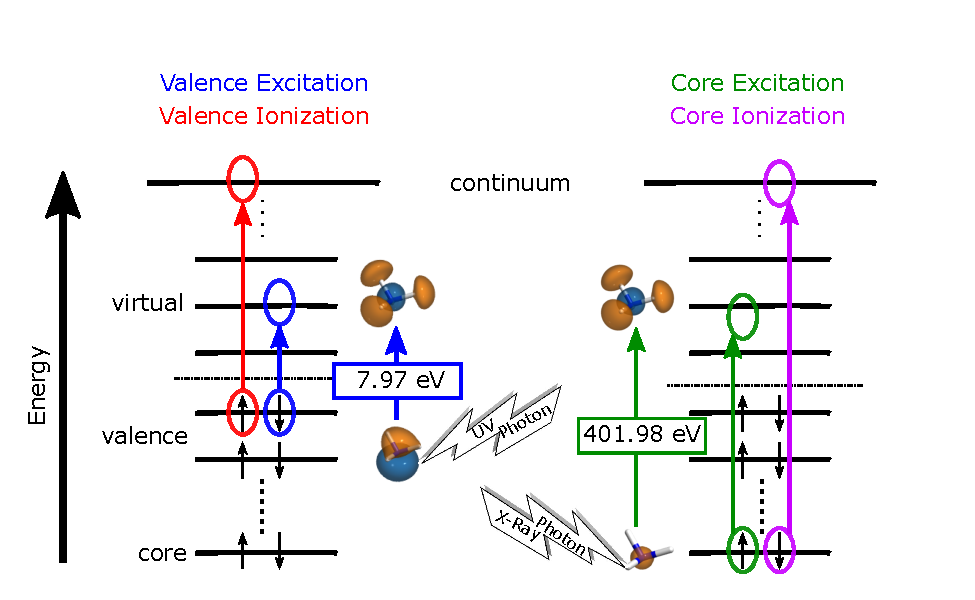
\includegraphics[scale=0.7]{photochem_graphic.pdf}
\caption{Sketch of the difference between UV and X-ray photo-absorption. The energies are not true to scale. The valence excitation and valence ionizaton processes are shown in blue and red respectively. The core excitation and core ionization processes are shown in green and purple respectively. An example is shown of the first valence and core excited state in ammonia (NH$_3$), the orbitals shown are hole and particle from orthogonality constrained density functional theory excited state computations at the B3LYP/3-21G level of theory.}
\label{fig:photochem}
\end{figure}

If we consider a closed-shell molecule, i.e. where all electrons are paired, when this molecule is not under the influence of any external radiation it is in its ground electronic state (S$_0$). Photons from impending radiation can excite the molecule from the ground state to an electronic excited state, promoting an electron from an occupied molecular orbital (MO) to a higher energy unoccupied MO (often referred to as a ``virtual'' orbital in quantum chemistry). The excitation energy ($\omega$) of the electronic excited state will depend upon the energy of the impending radiation. The lifetime of these electronic excited states are extremely short compared to the lifetime of molecular vibrations and thus these states can often be modeled properly within the vertical Franck-Condon approximation \cite{franck_elementary_1926,condon_theory_1926,condon_nuclear_1928,hazra_first_2004} where the electronic transition is assumed to occur without significant changes to the positions of the nuclei of the molecular system. The molecule eventually relaxes back down to its ground state level via a subsequent decay process such as fluoresence, \cite{maxwell_chlorophyll_2000,valeur_molecular_2012} phosphorescence, \cite{tanaka_observation_2005,romanovskii_phosphorescence_2000,cavar_fluorescence_2005} non-radiative relaxation, \cite{callomon_non-radiative_1972,de_mello_donega_non-radiative_1995} intersystem crossing, \cite{lamola_mechanisms_1965,hauser_intersystem_1991} and a myriad of other processes. \cite{zakrzewski_threshold_1984,meskers_relaxation_2000,vant_hof_zero-field_1976,hors_cross-relaxation_1982}

A unique class of electronic photo-excitations involves promotion of a core electron to a valence MO, the corresponding state is often referred to as core-excited (core-excited states). The electrons that constitute the ``core'' of a molecule are those occupying the lowest energy molecular orbitals. These MOs are not actively involved in bonding with the surrounding molecular environment and have orbital character similar to free-atom atomic orbitals (i.e. the 1s core orbital of NH$_3$ in Figure \ref{fig:photochem}). The number of MOs that compose the core is dependent upon the atomic number ($Z$) of the atom involved. For example, for lighter first-row elements in the periodic table, like oxygen, the 1s orbital is the only core orbital. However for heavier elements, like titanium, the 2s and 2p are also considered in the core level. Strong attractive Coulombic forces between the core electrons and the nuclei result in a large amount of energy being required to promote electrons from core levels. Thus, while ultraviolet (UV) or visible (VIS) photons are sufficient to excite valence electrons, high energy X-ray photons are required in order to excite core electrons. Figure \ref{fig:photochem} shows this process for both the valence and core cases respectively, and details the energy difference between the two in an example case of ammonia (NH$_3$). The first electronic valence excitation in ammonia has an excitation energy of 7.97 eV, meanwhile the first N core excitation has an excitation energy of 401.98 eV. It is clear that the high energy range, and unique nature of these transitions warrants an entire field of spectroscopy dedicated to its understanding.

\section{X-Ray Absorption Spectroscopy}
Core-excited states can be probed experimentally via X-ray absorption spectroscopy (XAS), a rapidly growing field that commonly makes use of synchrotron radiation in order to provide a tunable and intense X-ray beam source.\cite{snigirev_compound_1996,holch_new_2011} Tunability of the X-ray beam source allows it to scan a wide energy range throughout the X-ray region. Due to the large degree of energetic separation between the core and valence orbitals,\cite{politzer_separation_1976} scanning the X-ray beam through the binding energy of a core electron results in an abrupt increase in the absorption cross-section. This generates the so-called absorption ``edge'', with each unique edge region corresponding to a different core electron binding energy.\cite{stohr_nexafs_1992} The different edge regions are named using standard X-ray notation which is based on the principal quantum number of the excited electron; K for $n$=1, L for $n$=2, and M for $n$=3 (see Figure \ref{fig:xas_schematic}a).\cite{penner-hahn_x-ray_1999} Each edge is well separated from the rest of the absorption spectrum due to the dependence of the binding energy of core electrons on the charge of the nucleus. The fact that the edge position is dependent upon the atomic number ($Z$), XAS is often referred to as an ``element specific'' technique. For example, a typical K-edge resulting from oxygen core excitations is located at approximately 530 eV,\cite{yoon_oxygen_2002,parent_structure_2002} while the K-edge for nitrogen is located at approximately 400 eV.\cite{lambrecht_x-ray_1997,leinweber_nitrogen_2007} The existence of an absorption edge by itself has little relevance outside of simple elemental identification.\cite{cotte_synchrotron-based_2010} Fortunately the edge is not simply a discontinuous absorption increase, it has an abundance of structure (often referred to as ``fine structure'') throughout the different regions of the edge. Figure \ref{fig:xas_schematic}b shows a schematic drawing of a typical K-edge with the different regions of the fine structure highlighted. The first region of fine structure just before the edge is known as the pre-edge region. Although some organic 1s$\rightarrow$ $\pi^*$ transitions can populate this region, distinct features only arise in the case of transition metal complexes, where this region is populated by core transitions to unoccupied d-orbitals.\cite{yamamoto_assignment_2008,vedrinskii_pre-edge_1998,groot_1s_2009,roemelt_manganese_2012} The rising-edge region is composed of all other discrete core transitions of the system and has a distinct shape, that is typically dominated by intense 1s $\rightarrow$ $\pi^*$ transitions accompanied by weaker 1s $\rightarrow$ $\sigma^*$ transitions. The study of the fine structure that composes these two edge regions are the focus of near-edge X-ray absorption fine structure spectroscopy (NEXAFS).\cite{stohr_nexafs_1992} The last region of edge structure, the extended-edge region, is composed of signals past the ionization threshold of the core orbital in which core electrons are promoted to continuum (see Figure \ref{fig:photochem}). At this point the excited photoelectron has a high amount of energy, enough for its wavelength to be on the scale of interatomic distances. The resulting spectrum is a characteristic pattern of modulating local maxima and minima that correcpond to constructive and destructive interference between outgoing and backscattered photoelectron waves. As a result of this atomic-level sensitivity of the signal this region is sensitive to the radial distribution of electron density around the atom. The study of this signal, and its use to quantify geometric information such as bond lengths/coordination numbers is known as extended-edge X-ray absorption fine structure spectroscopy (EXAFS). \cite{lengeler_extended_1980,teo_exafs:_2012,gurman_rapid_1984,bunker_application_1983}

\begin{figure}
\centering
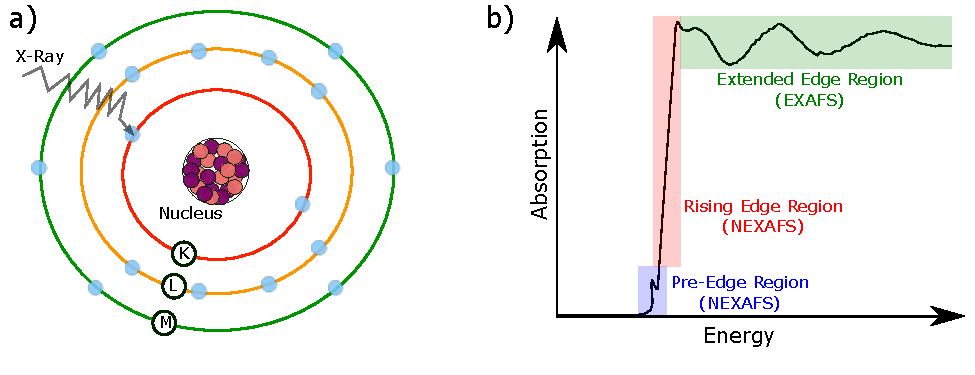
\includegraphics[scale=0.93]{XAS_schematic.pdf}
\caption{a) Schematic highlighting the X-ray absorption process, specifically shown here is an excitation of an electron from the first orbital shell (K-shell) of an arbitrary molecule. b) Drawing of the general shape of a K-edge X-ray absorption spectrum. The unique regions of the spectrum are marked and grouped with their corresponding spectroscopic method, either near-edge (NE) or extended-edge (E) x-ray absorption fine spectroscopy (XAFS).}
\label{fig:xas_schematic}
\end{figure}

With regard to the electronic structure of molecules, the near-edge region contains very useful information. \cite{garino_determination_2014,tourillon_electronic_1988} NEXAFS has been applied to a wide range of molecular systems including biological systems,\cite{zubavichus_nexafs_2004, zubavichus_nexafs_2009,samuel_nexafs_2017} small gas phase molecules,\cite{contini_gas-phase_2001,domke_carbon_1990,hudson_high-resolution_1994} organic thin-films,\cite{roy_structure_2005,hahner_near_2006,baldo_excitonic_1999} and semiconducting materials.\cite{guo_electronic_2011} For example, information regarding the orientation of organic molecules chemisorbed to surfaces can be obtained with NEXAFS. \cite{hoffmann_discovery_1990,stohr_bonding_1983,temprano_1d_2015,rastgoo-lahrood_post-synthetic_2016} One study investigated the adsorption structure of pyrazine (C$_4$H$_4$N$_2$) on a reconstructed Si(100) surface. \cite{lee_selective_2012} Through investigating changes in the polarization dependent NEXAFS spectrum, the geometry of the molecule relative to the surface normal could be deduced. NEXAFS can even be useful in explaining reaction mechanisms by using time-resolved X-ray spectroscopy.\cite{chen_probing_2005} A recent work by Attar et al. made use of time-resolved femtosecond NEXAFS in order to study the electrocyclic ring-opening reaction of 1,3-cyclohexadiene. \cite{attar_femtosecond_2017} Tracking the changes in the NEXAFS spectrum over time revealed strong mixing amongst the frontier orbitals and provided justification for the long postulated Woodward-Hoffman rules for pericyclic reaction mechanisms. \cite{day_aromaticity_1975}
Detailed interpretation of experimental X-ray absorption spectra requires knowledge of the relevant core excitation energies and excited state properties. Accurate quantum chemistry methods can often calculate electronic excited states and simulate the absorption spectrum of molecules. Along with interpretation of the properties and character of the transition, quantum chemistry calculations can yield plenty of useful information regarding the nature of electronic excited states. Many modern computational techniques have the capability of producing quantitatively accurate results regarding the excited states of systems of moderate size (less than 20 atoms). \cite{baeck_ab_2003,gwaltney_coupled-cluster_1998,shih_ab_1976,isborn_excited-state_2011} However, for the excited states of significantly larger systems, approximations must be made that represent a concession of accuracy for the sake of computational efficiency. \cite{fantacci_absorption_2003,de_angelis_electronic_2006} Utilizing quantum chemistry methods for the study of core-excited states encounters quite a few unique challenges. The most practical challenge they face from a purely computational perspective focuses on the eigenvalue solvers employed by many methods. Iterativive diagonalization algorithms are routinely employed as the eigenvalue solver in many quantum chemistry methods. \cite{gwaltney_simplified_1996,roos_new_1972,nakatsuji_structure_2001,mazur_application_2009} These approaches typically yield the lowest eigenvalue solutions and thus, tend to be efficient approaches for solving valence excited states. Core-excited states however, are much higher in energy. In order obtain solutions from the core region of the excitation spectrum, all underlying valence excited states must be calculated,\cite{imamura_time-dependent_2006} this is computationally inefficient in all cases and impossible for larger systems. Multiple strategies exist to overcome this algorithmic challenge, they typically revolve around target specific energy solutions \cite{besley_time-dependent_2010,peng_energy-specific_2015,lestrange_calibration_2015} or formally decoupling the space of core excitations from the space of valence excitations.\cite{ehlert_quest_2017,wenzel_calculating_2014} Both routes are viable options for overcoming this difficulty and the details of these approaches will be reviewed throughout the following section. Other challenges faced by quantum chemistry methods when calculating core-excited states are more physical in nature and have to do with the unique physics present in the core excitation mechanism. As stated previously, core electrons are tightly bound due to their close proximity to the nuclei and generation of a core hole causes significant orbital relaxation and a subsequent lowering of the total energy. Although orbital relaxation technically occurs in every excited state, the effect is less pronounced in valence excitations and is often times negligible in these calculations. To highlight this, a study by Triguero et al. \cite{triguero_separate_1999} investigated the sources of error in Koopmans approximation\bibnote{In Koopmans theorem the $i^{\rm th}$ Ionization potential is approximated by the corresponding energy eigenvalue of the canonical SCF equation $-\epsilon_i$.} of an ionization potential, . This error can be divided into three contributions: $R1$ ($<0$) due to orbital relaxation, $R2$ ($>0$) due to correlation,  and $R3$ ($<0$) due to the relaxation induced change in correlation. For valence ionizations, the relationship between the three sources of error is $-R1 \approx R2 \gg -R3$. However, for core ionizations this relationship becomes $-R1 \gg R2 \approx -R3$ with the error due to orbital relaxation becoming the dominant term. For example, Plakhutin et al. \cite{plakhutin_koopmans_2006} showed that for core ionization a nitrogen atom, $R1$ is on the order of 12-15 eV. \cite{plakhutin_koopmans_2006} Clearly this energy contribution is non-neglible for core-excited states and any quantum chemistry method striving for accurate energy calculations must consider this effect. Another consideration is the treatment of relativistic effects. Relativistic contraction of the core orbitals toward the nuclei results in a lowering of the core orbital energy while the valence orbital energies remain relatively uneffected. This results in an increase in excitation energy with respect to a nonrelativistic solution that is often non-negligible and becomes particularly important for core-excited states of heavier nuclei. 
\begin{table}
\centering
\caption{Non-relativistic (NR) and relativistic (R) energies (in eV) of the lowest lying core orbital and lowest unoccupied molecular orbital (LUMO) of water (H$_2$O) and silane (SiH$_4$) molecules calculated using spin-unrestricted Hartree--Fock (UHF) with the 3-21G basis set. Scalar relativistic effects are included by use of the 2$^{\rm nd}$ order Douglas-Kroll-Hess Hamiltonian.\cite{reiher_douglaskrollhess_2006} All calculations were performed using the ORCA software package.}
\begin{tabular}{ccccc}
\toprule
& \multicolumn{2}{c}{H$_2$O} & \multicolumn{2}{c}{SiH$_4$} \\ \cmidrule(lr){2-3} \cmidrule(lr){4-5}
& O 1s & LUMO & Si 1s & LUMO \\
\hline
NR-UHF & $-$555.88 & 7.17 & $-$1858.20 & 5.02\\
R-UHF & $-$556.34 & 7.16 & $-$1863.04 & 5.03\\
\bottomrule
\end{tabular}
\label{tab:rel_effects}
\end{table}
Table \ref{tab:rel_effects} shows orbital energies of the lowest lying core orbital and the lowest unoccupied molecular orbital (LUMO) for water (H$_2$O) and silane (SiH$_4$) molecules in a non-relativistic SCF calculation and a relativistic computation where scalar relativistic effects are taken into account using the Douglass--Kroll Hess Hamiltonian.\cite{reiher_douglaskrollhess_2006} The core orbital energy in H$_2$O lowers by 0.46 eV while the LUMO experiences negligible energy lowering of 0.01 eV. This effect becomes more pronounced with heavier elements, as the core orbital of silane experiences a relativistic contraction of 4.84 eV while it's LUMO raises in energy by only 0.01 eV. In the following section I will review the current theoretical approaches that have been applied to core-excited states and address how they approach the treatment and/or approximation the necessary components.

\section{Theoretical Approaches for Calculation of Core Excited States}
In the past, approaches for treatment of core-excited states were rare due to a lack of attention on XAS, however the advent of synchrotron radiation made these experiments more abundant and drove development throughout the years. This has lead to numerous computational approaches for calculating the properties of core-excited states. As discussed in detail in the previous section, core-excited states encounter a wealth of computational challenges including the algortihmic challenge of targeting the core region of the excitation spectrum and treatment of orbital relaxation and relativistic effects. This section will focus on reviewing theoretical approaches for the treatment of core-excited states within the framework of Hartree--Fock static exchange (HF-STEX),\cite{agren_direct_1994,hunt_excited_1969,zhang_nonlinear_2014,agren_direct_1997} time-dependent density functional theory (TDDFT), \cite{imamura_time-dependent_2006,besley_time-dependent_2007,lestrange_calibration_2015} and coupled cluster theory (CC).\cite{fransson_carbon_2013,besley_equation_2012,coriani_coupled-cluster_2012,coriani_asymmetric-lanczos-chain-driven_2012,myhre_near-edge_2016} For information regarding other noteworthy theoretical approaches including algebraic diagrammatic construction (ADC),\cite{wenzel_calculating_2014,wenzel_analysis_2015,wenzel_calculating_2014,wenzel_physical_2016} restricted active space self-consistent-field approaches (RASSCF),\cite{mochizuki_hf-stex_2001} configuration interaction,\cite{maganas_combined_2014,maganas_l-edge_2014,grimme_density_1996,asmuruf_calculation_2008} real-time time-dependent DFT (RT-TDDFT), \cite{lopata_linear-response_2012} and/or approaches using the Bethe-Salpeter equation,\cite{olovsson_near-edge_2009,vinson_theoretical_2012} I refer the reader to the existing literature on these topics. The focus here will be on treatment core-excitations relevant to K-edge applications, it is worth noting that there are numerous appraoches for the L-edge requires a more detailed theoretical treatment due to spin-orbit coupling,\cite{roemelt_combined_2013,ebert_l-edge_1996,maganas_first_2013} however this is outside of the scope of this dissertation. 

%A significant amount of progress has been made over the last few decades in order to make computations of core-excited states feasible and efficient in a plethora of different theories in quantum chemistry. As synchrotron facilities have become more powerful and plentiful the amount of high-quality X-ray absorption data has grown exponentially, inspiring more development in theory. Most modern techniques for the treatment of core-excitations fall into one of five classes that will be reviewed here: Hartree--Fock Static Exchange (HF-STEX), core valence separation (CVS), restricted excitation window (REW), energy specific (ES), or complex polarization propagator (CPP) methods. This review will focus primarily on methods used routinely in K-edge applications, there are more detailed multi-reference and relativistic methods in order to accurately treat the L-edge however those methods are outside the scope of this thesis. 
\subsection{Hartree-Fock Static Exchange}
HF-STEX (also known as improved virtual orbital Hartree--Fock) is a state specific Hartree--Fock approach in which a simplified configuration interaction singles expansion is performed to obtain excited states from a reference determinant that has been optimized for a core hole potential.\cite{agren_direct_1994,hunt_excited_1969,zhang_nonlinear_2014,agren_direct_1997} The reference determinant is constructed by performing an open-shell HF calculation in which an electron is removed from the core region of an N-electron system. Variational optimization of this (N$-$1)-electron state produces relaxed orbitals into the reference, providing an improved decription of the occupied and virtual HF orbitals. This direct inclusion of relaxation effects is one of the strongest advantages of HF-STEX based methods and is the starting approximation for practically every state specific/variational approach for core-excited state. The validity of this approximation supported by the large energy separation between the core and valence orbitals as well as the spatial separation of core orbitals on different atomic centers within a molecule. Let us consider an excitation from core orbital $j$ to valence orbital $b$ from a closed shell reference state $|\Psi_0\rangle$, the STEX eigenvalue problem can be defined as
\begin{equation}
\label{eq:HFSTEX_eig}
F^j \phi_b = \epsilon_{jb} \phi_b,
\end{equation}
where $F^j$ is the HF-STEX Fock operator
\begin{equation}
F^j = h + \sum_{i \neq j} (2J_i - K_i) + J_j - K_j.
\end{equation}
It should be noted that the excited states obtained from the open-shell HF reference are not orthogonal to the HF ground state and thus overlaps between the states must be accounted for. After accounting for non-orthogonality, the HF-STEX eigenvalue equation can be solved and the excitation energies ($\omega_{jb}$) can be obtained by adding the core ionization potential to the eigenvalue obtained in Equation \ref{eq:HFSTEX_eig}. The oscillator strengths are evaluated in terms of the excitation energy and the transition dipole moment as
\begin{equation}
f_{jb} = \frac{2}{3} \omega_{jb}|\langle \Psi_0|\vec{r}|\Psi_{jb}\rangle|^2,
\end{equation}
With regard to the performance of HF-STEX, it produces XAS spectra that are in acceptable quantitative agreement with experimental results. HF-STEX oscillator strengths also provide a good qualitative comparison with experimental line intensities.

Excited state solutions within HF-STEX can be best understood as an approximate solution to the random phase approximation (RPA).  Lets consider a general RPA excitation operator $\hat{T}_I$ for an excited state $I$ within the Tamm-Dancoff approximation (TDA):\cite{hirata_time-dependent_1999}
\begin{equation}
\hat{T}_I = \sum_{i,a} (\mathbf{X}_{ia,I}\hat{a}^{\dagger}_{a}\hat{a}_i),
\end{equation}
where $\mathbf{X}$ is the eigenvector of the RPA equation within the TDA, while $i$ and $a$ are indices that run over the ground state occupied and virtual orbitals respectively. This type of excitation operator contitutes what is known as a ``multi-channel'' approach, essentially a linear combination of single excitations that accounts for the interaction of different excitation channels. For HF-STEX, this excitation operator is limited to a restricted sum over single excitations from a given orbital $j$, also known as a ``single-channel'' approach
\begin{equation}
\hat{T}_I = \sum_{a} (\mathbf{X}_{ja,I}\hat{a}^{\dagger}_{a})\hat{a}_j,
\end{equation}
It should be noted that this would be an extremely poor approximation for valence-excited states as multiple excitation channels tend to be clustered within a fairly small energy range (potentially less than 1 eV). However, due to the large energy separation of core orbitals, it is possible to obtain an accurate simulation of the XAS spectrum within a single channel approximation. 

The attractive features of this theory are however hampered by two main challenges.  The first is the difficulty of converging the open-shell SCF reference state necessary to build the STEX Hamiltonian. It is notoriously difficult to converge on the desired core hole state. However, there are solutions to this problem that can aide convergence of the core hole state, most notably the maximum overlap method.\cite{besley_self-consistent-field_2009} The second challenge with HF-STEX lies in the non-orthogonality of the excited states within the core-hole potential which requires explicit wavefunction overlaps to be accounted for. 
\subsection{Linear Response Time-Dependent Density Functional Theory Approaches}
With regard to computational cost, linear response time-dependent density functional theory (TDDFT) remains one of the most attractive options for calculating electronic excited states in a wide variety of systems. Within TDDFT, excitation energies ($\omega$) are calculated via solutions to the following non-Hermitian eigenvalue equation:
\begin{equation}
\label{eq:tddft_eigenvalue_equation}
\begin{pmatrix}
\mathbf{A} & \mathbf{B} \\
\mathbf{B^{\dagger}} & \mathbf{A^{\dagger}} 
\end{pmatrix} 
\begin{pmatrix}
\mathbf{X}\\
\mathbf{Y}
\end{pmatrix}
= \omega
\begin{pmatrix}
\mathbf{1} & 0 \\
0 & -\mathbf{1}
\end{pmatrix}
\begin{pmatrix}
\mathbf{X} \\
\mathbf{-Y}
\end{pmatrix},
\end{equation}
where the matrices $\mathbf{A}$ and $\mathbf{B}$ are given by
\begin{align}
\label{eq:A_matrix}
A_{ai\sigma,bj\tau} &=  \delta_{ij} \delta_{ab} \delta_{\sigma\tau}(\epsilon_{a\sigma} - \epsilon_{i\tau}) + (ia\sigma|jb\tau) + (ia\sigma|f_{\rm XC}|jb\tau), \\
\label{eq:B_matrix}
B_{ai\sigma,jb\tau} &= (ia\sigma|jb\tau) + (ia\sigma|f_{\rm XC}|jb\tau),
\end{align}

for occupied orbitals $i,j,...$, virtual orbitals $a,b,...$, spin indices $\sigma$ and $\tau$, and energy eigenvalues $\epsilon$. The second term in Equation \ref{eq:A_matrix} is a two-electron integral and can be expressed explicitly in terms of a set of Kohn--Sham orbitals ($\phi_i$) as:

\begin{equation}
(ia\sigma|jb\tau) = \int \int \phi^*_{i\sigma}(\mathbf{r}_1)  \phi^*_{a\sigma}(\mathbf{r}_1) \frac{1}{r_{12}} \phi^*_{j\tau}(\mathbf{r}_2) \phi^*_{b\tau}(\mathbf{r}_2) d\mathbf{r}_1 d\mathbf{r}_2,
\end{equation}

while the third term is what is known as the exchange correlation kernel which can be expressed as the functional derivative

\begin{equation}
(ia\sigma|f_{\rm XC}|jb\tau) = \int \phi^*_{i\sigma}(\mathbf{r}_1)  \phi^*_{a\sigma}(\mathbf{r}_1) \frac{\delta^2 E_{XC}}{\delta \rho{\sigma}(\mathbf{r}_1 \delta \rho_{\tau}(\mathbf{r}_2)} \phi^*_{j\tau}(\mathbf{r}_2) \phi^*_{b\tau}(\mathbf{r}_2) d\mathbf{r}_1 d\mathbf{r}_2,
\end{equation}
where $E_{\rm XC}$ is the exchange correlation functional. Within the Tamm-Dancoff approximation (TDA),\cite{fetter_quantum_1971} Equation \ref{eq:tddft_eigenvalue_equation} reduces to a Hermitian eigenvalue equation $\mathbf{A}\mathbf{X} = \omega\mathbf{X}$. Eliminating the off diagonal elements $\mathbf{B}$ greatly reduces the computational cost of solving the equation and makes the theory formally similar to configuration interaction singles. Many modern implementations of TDDFT make use of some form of the Davidson algorithm which iteratively diagonalizes a subspace of the Hamiltonian yielding its lowest (highest) eigenvalues in a bottom-up (top-down) fashion. This is a reasonable and efficient choice when the excitations of interest are valence excitations. However, excitations involving the lower energy core orbitals introduce a significant computational challenge since there is typically a plethora of valence excitations below the target core excitations, making the algorithm prohibitively. Overcoming this prohibitive expense is the primary motivation of methods developed to calculate core excitations within the TDDFT. 
\subsubsection{Restricted Excitation Window TDDFT}
Originally proposed by Stener et al.,\cite{stener_time_2003} restricted excitation window TDDFT (REW-TDDFT) is a modification to the standard TDDFT algorithm that only allows electrons to be excited from a subset of core orbitals. \cite{imamura_time-dependent_2006,besley_time-dependent_2007} This approximation is physically motivated by the large energy separation of core levels of different atomic species, and the large spatial separation of core orbitals on different atoms. This is normally done in one of two ways: (1) Core orbitals of interest are selected directly via orbital localization schemes for equivalent atoms (i.e. selecting all MOs that have primarily oxygen 1s character) or (2) Use an orbital energy (energy difference) cutoff in order to filter out any orbitals (orbital pairs) that lie above (below) the user provided energy threshold. The latter option is by far the most popular and has become commonplace for TDDFT implementations in modern quantum chemistry packages. 

Although REW-TDDFT allows for the computation of core excited states, it naturally inherits the issues of standard TDDFT calculations, namely the large dependence on the choice of exchange-correlation functional. This has lead to development of a new class of functionals for use with REW-TDDFT known as short range corrected (SRC) functionals which are modified versions of long range corrected (LRC) functionals used for charge transfer excitations in TDDFT. The LRC exchange correlation functional can be expressed as
\begin{equation}
E^{\rm LRC}_{\rm XC} = E^{\rm SR-DFT}_{\rm X} + E^{\rm LR-HF}_{\rm X} + E^{\rm DFT}_{\rm C},
\end{equation}
combining a DFT exchange in the short-range ($E^{\rm SR-DFT}_{\rm X}$), with Hartree--Fock exchange in the longer-range ($E^{\rm LR-HF}_{\rm X}$), and DFT correlation energy ($E^{\rm DFT}_{\rm C}$). SRC functionals modify this general form to include a certain portion of Hartree--Fock exchange in the short range as well, where the SRC exchange-correlation energy ($E^{\rm SRC}_{\rm XC}$) can be expressed as
\begin{equation}
E^{\rm SRC}_{\rm XC} = c_{\rm X}E^{\rm SR-HF}_{\rm X} + E^{\rm SR-DFT}_{\rm X} + E^{\rm LR-HF}_{\rm X} + E^{\rm DFT}_{\rm C}, 
\end{equation}
where $c_{\rm X}$ is a parameter that can be optimized. The major drawback with this method is that the amount of HF exchange in the functional must be re-optimized for any given system, which can be cumbersome and limits its reliability in application to novel problems. 
\subsubsection{Energy Specific TDDFT}
Starting from the non-Hermitian eigenvalue problem shown in Equation \ref{eq:tddft_eigenvalue_equation}, this form is often placed into the following equivalent Hermitian eignvalue equation
\begin{equation}
(\mathbf{A} - \mathbf{B})^{1/2} (\mathbf{A} +\mathbf{B}) (\mathbf{A} - \mathbf{B})^{1/2} \mathbf{T} = \omega^2 \mathbf{T},
\end{equation}
where $\mathbf{T} = (\mathbf{A} - \mathbf{B})^{-1/2} (\mathbf{X} + \mathbf{Y})$. Energy Specific TDDFT (ES-TDDFT) \cite{lestrange_calibration_2015} aims to solve this Hermitian eigenvalue problem utilizing a ``growing window'' algorithm that starts from a set of trial vectors $\mathbf{C}$ associated with orbital pairs whose orbital energy difference are above a given threshold. A subspace $\mathbf{\tilde{M}}$ is then created using the trial vectors,
\begin{align}
\mathbf{\tilde{M}}^+ &= \mathbf{C^T} (\mathbf{A} +\mathbf{B})\mathbf{C} \\
\mathbf{\tilde{M}}^- &= \mathbf{C^T} (\mathbf{A} -\mathbf{B})\mathbf{C} \\
\mathbf{\tilde{M}} &= (\mathbf{\tilde{M}} ^-)^{1/2} (\mathbf{\tilde{M}} ^+) (\mathbf{\tilde{M}}^-)^{1/2},
\end{align}
Direct diagonalization is performed only in the subspace $\mathbf{\tilde{M}}$, which generates a new set of eigenvalues $\tilde{\omega}$ and eigenvectors $\tilde{T}$. Only those eigenvectors associated with eigenvalues above the user defined threshold are kept. These eigenvectors are then projected back onto the full MO space in order to calculate a residual, any new eigenvectors with significant amplitude are then added as a trial vector for the next iteration (hence the term ``growing window''). A new subspace is constructed from the expanded trial space and the process continues self-consistently until the residual is below a user-defined threshold.

Since this method checks the residual of the subspace against the full MO space, the final results that are obatained are true solutions of the TDDFT equations. Similar to REW-TDDFT, however, it inherits the functional dependence of TDDFT for the calculation of core excited states.

\subsection{Coupled Cluster Approaches}
The coupled-cluster wavefunction ($\Psi_{\rm CC}$) can be defined as an exponential expansion of a closed 
shell HF reference ($\Psi_{\rm HF}$)
\begin{equation}
|\Psi_{\rm CC}\rangle = e^{\hat{T}}|\Psi_{\rm HF} \rangle,
\end{equation}
where $\hat{T}$ is known as the cluster operator can be expressed as a linear combination of single, double, triple, etc. excitations, up to N-fold excitations for a general N-electron system
\begin{equation}
\hat{T} = \hat{T}_1 + \hat{T}_2 + \hat{T}_3 + ... + \hat{T}_N.
\end{equation}
Where each individual excitation operator is composed of cluster amplitudes ($t_{\mu}$) and excitation operators ($\hat{\tau}_{\mu}$) that represent excitations from occupied orbitals (i,j,k,...) to virtual orbitals (a,b,c,...)
\begin{equation}
\hat{T} = \sum_{\mu} t_{\mu} \hat{\tau}_{\mu} = \sum^{\rm occ}_{i > j > k> ...} \sum^{virt}_{a > b > c > ...} t^{abc...}_{ijk...} \hat{\tau}^{abc...}_{ijk...}.
\end{equation}
The total energy (E) and amplitudes ($\Omega_{\mu}$) of the ground state can then be determined by projections onto the reference state and onto a manifold of excitations out of the reference state
\begin{align}
E &= \langle \Psi_{\rm HF} | e^{- \hat{T}}\hat{H} e^{\hat{T}} |  \Psi_{\rm HF} \rangle, \\
\Omega_{\mu} &= \langle \Psi_{\mu} | e^{- \hat{T}}\hat{H} e^{\hat{T}} |  \Psi_{\rm HF} \rangle = 0.
\end{align}
The truncation of the cluster operator $\hat{T}$ gives rise to the different ``levels'' of coupled cluster theory:
\begin{align}
{\rm CCS}&: \hat{T}_1 \\
{\rm CCSD}&: \hat{T}_1 + \hat{T}_2 \\
{\rm CCSDT}&: \hat{T}_1 + \hat{T}_2 + \hat{T}_3 \\
{\rm CCSDTQ}&: \hat{T}_1 + \hat{T}_2 + \hat{T}_3 + \hat{T}_4  \\
\nonumber
\vdots
\end{align}
Within coupled-cluster theory, excited states can be obtained via a linear-response approach as well as a state-specific approach. Both approaches have challenges that must be overcome in order to calculate core-excited states. These methods for calculating core-excited states will be reviewed here.
\subsubsection{Linear-Response Coupled Cluster Theory}
Within coupled-cluster linear response theory,(CC-LR) excitation energies ($\omega_{k}$) are obtained by solving an asymmetric eigenvalue equation to obtain right ($\mathbf{R}_k $) and left ($\mathbf{L}_k$) eigenvectors, commonly referred to as excitation and de-excitation operators respectively
\begin{align}
\label{eq:right_cc}
\mathbf{AR_k} &= \omega_k \mathbf{R_k}, \\
\label{eq:left_cc}
\mathbf{L_kA} &= \omega_k \mathbf{L_k},
\end{align}
where the left and right eigenvalues are orthogonal ($\mathbf{L_iR_k} = \delta_{ik}$), and A is a Jacobian matrix that is defined as the gradient of the cluster amplitudes
\begin{equation}
A_{\mu \nu} = \frac{\partial \Omega_{\mu}}{\partial t_\nu},
\end{equation}
Many general schemes to iteratively solve Equations \ref{eq:right_cc} and \ref{eq:left_cc} have been introduced for excited state calculations. These methods typically rely on using HF orbital energy differences to select guess unit vectors for specific occupied to virtual excitations. One fatal flaw that many methods encounter when trying to calculate core-excitations, is that the iterative solver will converge onto the lowest energy eigenvalues and eigenvectors even if the starting unit vectors are chosen for higher energy excitations. To overcome this difficulty, Coriani and Koch introduced a novel approach to iteratively solving Equations \ref{eq:right_cc} and \ref{eq:left_cc} using an asymetric Lanczos algorithm.\cite{coriani_coupled-cluster_2012,coriani_asymmetric-lanczos-chain-driven_2012} This approach employs a tridiagonal representation $\mathbf{T}$ of the Jacobian matrix $\mathbf{A}$. 
\begin{equation}
\mathbf{T} = \mathbf{P^T A Q},
\end{equation}
where $\mathbf{P^TQ} = \mathbf{1}$. The diagonalization of $T$ is truncated at a dimension that is greatly reduced compared to the full dimension of possible excitations, generating an effective excitation spectrum. Using this approach the excitation spectrum converges to the exact excitation spectrum from the bottom or the top, i.e. higher energy starting vectors do converge on the higher energy. 
\subsubsection{Equation-of-Motion Coupled Cluster Singles and Doubles}
Within the context of EOM-CCSD, it is conveniant to define a normal ordered Hamiltonian ($H_N$) that can be defined as
\begin{equation}
\hat{H}_N = e^{-\hat{T}}\hat{H}e^{\hat{T}} - E,
\end{equation}
this normal ordered Hamiltonian is then used to build the matrix elements of the EOM-CCSD Hamiltonian 
\begin{align}
\nonumber
\hat{H}_{\rm EOM-CCSD} &= 
\begin{bmatrix}
\hat{H}^{\rm SS} & \hat{H}^{\rm SD} \\
\hat{H}^{\rm DS} & \hat{H}^{\rm DD}
\end{bmatrix} \\
\nonumber
\hat{H}^{\rm SS} &= \langle \Phi_{i}^{a} | \hat{H}_N | \Phi_{k}^{c} \rangle \\
\nonumber
\hat{H}^{\rm SD} &= \langle \Phi_{i}^{a} | \hat{H}_N | \Phi_{kl}^{cd} \rangle \\
\nonumber
\hat{H}^{\rm DS} &= \langle \Phi_{ij}^{ab} | \hat{H}_N | \Phi_{k}^{c} \rangle \\
\hat{H}^{\rm DD} &= \langle \Phi_{ij}^{ab} | \hat{H}_N | \Phi_{kl}^{cd} \rangle,
\end{align}
where $|\Phi_{i}^{a} \rangle$ and $|\Phi_{ij}^{ab} \rangle$ are the singly and doubly excited determinants respectively. This EOM-CCSD Hamiltonian is then diagonalized using a modified Davidson algorithm to obtain the excitation energy eigenvalue spectrum. Similar to CC-LR, EOM-CCSD suffers from a feasibility problem as the high energy core-excited states can only be obtained after first obtaining a series of lower energy solutions. The need to solve for the full dimension of excitations in order to reach the core-excited states of interest causes standard diagonalization techniques to become computationally expensive for all cases and impossible for reasonably large cases. This issue can be handled in a similar way to the energy specific TDDFT method outlined above, to yield an energy specific EOM method (ES-EOM-CCSD)\cite{peng_energy-specific_2015}

\begin{comment}
\subsection{Real-Time Time-Dependent Density Functional Theory}
An alternative time-dependent density functional theory approach is real-time TDDFT (RT-TDDFT). In RT-TDDFT the density matrix is propagated in time utilizing the time dependent form of the Kohn-Sham equation. [CITE] This is done by solving the following equation of motion
\begin{equation}
\label{eq:real_time_EOM}
i \frac{\partial \mathbf{D}(t)}{\partial t} = [\mathbf{F}(t), \mathbf{D}(t)]
\end{equation}
where $\mathbf{D}(t)$ is the time dependent one-electron density matrix and $\mathbf{F}(t)$ is the time dependent Fock matrix which can be expressed in the following form for the case of hybrid exchange-correlation functionals
\begin{equation}
\label{eq:time_dependent_fock}
\mathbf{F}[\mathbf{D}(t)] = \mathbf{H}^{\rm core} + \mathbf{J}[\mathbf{D}(t)] + \mathbf{E}_{\rm XC} [\rho(\mathbf{r},t)]- \mathbf{\mu} \mathbf{V}^{\rm ext}(t)
\end{equation}
where $\rho(\mathbf{r}, t)$ is the time-dependent electron density, $\mathbf{\mu}$ is the dipole matrix, and $\mathbf{V}^{\rm ext}(t)$ is the applied external potential. The coefficients $\alpha$, $\beta$, and $\gamma$ are parameters that control the amount of Hartree--Fock and DFT exchange, respectively. It should be noted that the expression in Equation \ref{eq:time_dependent_fock} only considers the coupling of the dipole moment with the external potential, this is valid within the ``long wavelength'' approximation where it is assumed that the photon is much longer than the system size. This approximation is almost always valid for UV/Vis photons and X-ray photons of organic molecules, however, it can breakdown for higher energy core excitations in transition metals. At which point it will be necessary to consider higher order multipole moments beyond the electric dipole approximation. [CITE]

Solutions to the real-time approach involve integrating Equation \ref{eq:real_time_EOM} in order to obtain the time-dependent density matrix.  The Magnus expansion is a popular integrator for obtaining these solutions. [CITE] Within this expansion the density matrix is propagated through time via a unitary propagator which conserves idempotency. The exact unitary propagator for Equation \ref{eq:real_time_EOM} is given as
\begin{equation}
\mathbf{U}(t + \Delta t, t) = T \ {\rm exp}\{-i \int^{t+\Delta t}_t \mathbf{F}(\tau) d\tau\},
\end{equation}
such that the time propagation of the density matrix can be written as
\begin{equation}
\mathbf{D}(t + \Delta t) = \mathbf{U}(t + \Delta t, t) \mathbf{D}(t) \mathbf{U}^{\dagger}(t + \Delta t, t),
\end{equation}
where $\Delta t$ is the time-step and $T$ is a time-ordering operator that orders the operations associated with later times from those associated with earlier times. Due to the explicit time dependence of the Fock matrix it is impossible to evalute this propagator directly. However, it can be written in terms of a Magnus expansion
\begin{equation}
 T \ {\rm exp}\{-i \int^{t+\Delta t}_t \mathbf{F}(\tau) d\tau\} = e^{\Omega_1 + \Omega_2 + ... +\Omega_M},
\end{equation}
where $M$ is the total number of Magnus terms $\Omega_i$. The Magnus expansion is typically truncated at $M=1$ such that the unitary propagator can be approximated as
\begin{align}
\mathbf{U}(t + \Delta t, t) &\approx e^{\Omega_1} \\
\Omega_1 &\approx -i\mathbf{F}(t + \Delta t/2).
\end{align}
Within this form, the Fock matrix at a future time is guessed via linear extrapolation and solved for iteratively. This allows for the following explicit form of the time propagation of the density matrix
\begin{equation}
\mathbf{D}(t + \Delta t) = e^{-i\mathbf{F}(t+\Delta t/2)\Delta t} \mathbf{D}(t) e^{-i\mathbf{F}(t+\Delta t/2)\Delta t}.
\end{equation}
Core excitations typically have oscillations on the attosecond timescale, thus time steps on the tenth of an attosecond time scale must be taken to ensure accuracy within this region. An optical absorption spectrum can be obtained from a real-time simulation via a Fourier transform of the time-dependent dipole moment that results from a small applied electric field. For excitations on longer time scales, a Gaussian electric field can be chosen, however to accomodate the short time scales of core excitations a delta function perturbation is typically applied [CITE]
\begin{equation}
\mathbf{E}_{\delta}(t) = \kappa \delta(t) \mathbf{\hat{d}}.
\end{equation}
\end{comment}
%\subsection{Theoretical Treatment of X-Ray Absorption Spectroscopy}
%Our starting point for an introduction to the theory of XAS is the simplification of the many electron problem into a generalized independent particle approximation based on the standard hole/electron quasiparticle picture. This simplifies the many-body theory into an effective independent electron approximation of an electronic excitation from initial state $|i\rangle$ to final state $|f\rangle$. Within this simplified picture, the absorption coefficient $\mu$ for a given photon energy $\omega$ can be expressed as
%\begin{equation}
%\mu(\omega) \approx \sum_f | \langle i | d | f \rangle |^2 \delta(\hbar \omega + E_i - E_f)
%\end{equation}
%where $\hbar \omega + E_i$ is the energy of the photoelectron and $d$ is the dipole coupling to the x-ray field. This equation is essentially a sum over final states $|f\rangle$. The composition of the final states are important to the theory and must provide an accurate representation of the excited state, however their construction in this case is not obvious. Many modern one-electron theories construct the final states in a self-consistent potential that includes a core-hole, this procedure is known as the Hartree--Fock static exchange approximation (HF-STEX). This approximation is physically motivated by the large energy separation of core levels of different atomic species, and the large spatial separation of core orbitals on different atoms. Allowing for a single excitation to be modeled in terms of relaxed orbitals from a given core-hole state. Within this approximation, $\psi_f$ is the wavefunction representing the final state with $h^{\prime}$ as the Hamiltonian of the core-hole potential, yielding the following eigenvalue equation
%\begin{equation}
%h^{\prime} \psi_f = E \psi_f
%\end{equation}
%where E represents the final state energies, and $h^{\prime}$ has the following form
%\begin{equation}
%h^{\prime} = \frac{p^2}{2m} + V^{\prime}_H + \sum(E)
%\end{equation}
%where the first term is the kinetic energy, $V^{\prime}_H$ is the Hartree potential of the core-hole state and $ \sum(E)$ is the self-energy term. This quantity is a complex valued, dynamically screened exchange interaction that accounts for the many body effects of extrinsic loses that occur due to the propagation of the photoelectron. $ \sum(E)$ is analogous to the exchange correlation potential of density functional theory, essentially containing all information not captured in the kinetic and potential term. Within GW theory, $ \sum(E)$ has been effectively approximated and provides accurate results for EXAFS spectroscopy. However, this term is overestimated for near-edge applications and thus further treatment is necessary.
%\subsection{Near-Edge X-ray Absorption Fine Structure}
%As with any form of photo-electron spectroscopy the interpretation of XAS spectroscopy relies on the Beer-Lambert law which relates the exponential decrease of the intensity ($I$) of the transmitted beam with respect incident beam intensity ($I_0$):
%\begin{equation}
%I = I_0 e^{-\mu D}
%\end{equation}
%where $D$ is the sample thickness and $\mu$ is what's known as the linear absorption coefficient which is related to the absorption cross-section, $\sigma_i$, of the $n$ unique chemical elements present in the sample
%\begin{equation}
%\mu = \frac{1}{V} \sum^n_{i = 1} \sigma_i
%\end{equation}
%where $V$ is the volume of the sample. Interpretation of the spectrum requires analysis of the position, intensity, and spape of peak features. As stated earlier, the position of peak features an energy specific signature of the absorbing atom. However, the technique is sensitive enough to differentiate between the same element in unique chemical environments.
%\begin{figure}
%\centering
%\includegraphics[scale=0.5]{chromium_k_edge.png}
%\caption{NEXAFS spectra at the Cr K-edge of four unique Cr(III) containing compounds. Experimental spectra are shown as solid lines, theoretical spectra are shown as dotted lines and are calculated using multiple scattering theory inside the FEFF8 code.[CITE] All data is from ref [CITE]}
%\label{fig:chromium_k_edge}
%\end{figure}
%For example, Figure \ref{fig:chromium_k_edge} shows the different spectra for four different Cr(III) containing metal complexes. Although all of the Cr K-edge spectra appear in the same region (5980 - 6050 eV), each unique complex has a different spectral profile in terms of peak positions and lineshapes. This shows that NEXAFS is sensitive to differences in the electronic structure, even the structurally similar CrF$_3$ and CrCl$_3$ have drastically different K-edge footprints. The same is true of atoms at different oxidation states, when increasing oxidation the edge tends to shift toward higher energy. This makes NEXAFS an excellent tool to check the valence state of atoms. 

%The K-edge, which consists of excitations of 1s electrons forms a rich structure for any atom that serves as a resource to interpret the unoccupied states of the electronic structure. The L-Edge is more complex to interpret, however is just as powerful in interpreting information about a molecules electronic structure. The complexity arises from the degeneracies that exist at the 2p electronic level, this introduces an element of strong electron correlation and causes splitting in the spectrum related to spin-orbit coupling between the occupied p-orbitals and unoccupied 3d states. 

\section{Orthogonality Constrained Density Functional Theory}
In this section, I review orthogonality constrained density functional theory (OCDFT) as a general approach to electronic excited states. OCDFT belongs to a unique class of density functional approaches whose main goal is to study excited states without using a time-dependent formulation, otherwise known as time independent density functional theory (TIDFT). \cite{samal_exploring_2006,ayers_time-independent_2009} This class of methods aim to provide an alternative to TDDFT which has been known to struggle in cases of charge transfer and Rydberg excited states due to inadequacies of approximate exchange correlation functionals. \cite{zhang_challenge_1998,cohen_insights_2008}

OCDFT is a variational formulation of DFT for the calculation of excited states.\cite{evangelista_orthogonality_2013} Unique to the theory is the explicit enforment of constraints that guarantee orthogonality while allowing the MOs to fully relax. This draws inspriation from two TIDFT theories: 
\begin{itemize}
\item The variational TIDFT approach of Levy and Nagy which provides the theoretical framework for a universal excited state density functional,\cite{ayers_time-independent_2012} thereby justifying the variational optimization of an excited state in DFT.
\item The constrained DFT (CDFT) approach of Van Voorhis and coworkers \cite{kaduk_constrained_2012} which provides a framework for studying systems within Kohn--Sham DFT that have an arbitrary constraint on their density.
\end{itemize} 
The remainder of this section will provide a brief introduction to the theory, following this introduction will be a discussion of the features of the theory that specifically make it an attractive choice for the calculation of core-excited states.
\subsection{Original Formulation via Constrained Variational Minimization}
Within a generalized Kohn--Sham (KS) framework, an $n$-electron system can be represented in terms of an auxiliary system of noninteracting electrons. \cite{hohenberg_inhomogeneous_1964,kohn_self-consistent_1965} The KS auxiliary system can be represented by a single Slater determinant 
\begin{equation}
|\Phi\rangle = | \phi_1, \phi_2, ..., \phi_n \rangle,
\end{equation}
which is constructed from a set of KS orbitals \{$\phi_i$\}. The total ground state electronic energy of the KS system can be expressed as
\begin{equation}
E_{\rm KS}[\{\phi_i\}] = - \frac{1}{2} \sum^{\rm occ}_i \langle \phi_i| \bigtriangledown^2 | \phi_i \rangle + \int d\mathbf{r} \nu(\mathbf{r}) \rho(\mathbf{r}) + J[\rho] + E^{\prime}_{\rm XC}[\rho],
\end{equation}
where the first term is the kinetic energy contribution, the second term is the contribution of the external potential, while $J[\rho]$ and $E^{\prime}_{\rm XC}[\rho]$ are the Coulomb and exchange-correlation contribution respectively. In general, an excited state can be computed by a constrained minimization of the expectation value of the Hamiltonian ($\hat{H}$) over all the wave funtions orthogonal to the ground state $\Psi$:
\begin{align}
E^{\prime} &= \min_{\rho^{\prime}}\left\{\min_{\substack{\Psi^{\prime} \rightarrow \rho^{\prime} \\ \Psi^{\prime} \perp \Psi}} \langle \Psi^{\prime}| \hat{H} | \Psi\rangle \right\} \\
&= \min_{\rho^{\prime}}\left\{ \int d\mathbf{r} \nu(\mathbf{r}) \rho(\mathbf{r}) + F^{\prime}[\rho^{\prime}]\right\},
\end{align}
where $F^{\prime}[\rho^{\prime}]$ minimizes the sum of the kinetric energy ($\hat{T}$) and electron-electron repulsion. In the spirit of the variational TIDFT of Levy and Nagy, OCDFT introduces a ficticious KS system of noninteracting electrons with density $\rho^{\prime}_s$ which maps to the excited state density of the real interacting system $\rho^{\prime}$ and can be described by a unique Slater determinant $\Phi^{\prime}$. The excited state solution is obtained via a \textit{constrained minimization} subject to an orthogonality constraint on the auxiliary wavefunctions
\begin{equation}
\langle \Phi^{\prime}|\Phi \rangle = 0,
\end{equation}
Direct imposition of this orthogonality constraint avoids the excited state wavefunction from collapsing to the ground state solution. The OCDFT energy functional for the excited state is then expressed as
\begin{equation}
E^{\prime}_{\rm OCDFT}[\{\phi^{\prime}_i\}] = - \frac{1}{2} \sum^{\rm occ}_i \langle \phi^{\prime}_i| \bigtriangledown^2 | \phi^{\prime}_i \rangle + \int d\mathbf{r} \nu(\mathbf{r}) \rho^{\prime}(\mathbf{r}) + J[\rho^{\prime}] + E_{\rm XC}[\rho^{\prime}],
\end{equation}
Note that the exchange-correlation functional $E_{XC}$ is approximated with the ground state functional evaluated at the excited state density. This is an adiabatic approximation for the excited state and is discussed in more detail in Ref. \citenum{evangelista_orthogonality_2013}. 
\subsection{Attractive Features of OCDFT for Core Excitations}
This section will focus on the features of orthogonality constrained density functional theory that make it an attractive candidate as a theory for core excitations. Three features stand out the most and will be covered in more detail in this section:
\begin{itemize}
\item Full inclusion of orbital relaxation effects through variational optimization of Kohn--Sham orbitals.
\item Variational stability of the $\Delta$SCF procedure due to imposition of orbital orthogonality.
\item Computational cost and scaling comparable to time-dependent density functional theory.
\end{itemize}
Having established itself as a stable, cheap, and accurate theory for electronic excited states the extension of this theory for the treatment of core excited states seemed like a logical progression.
\subsubsection{Orbital Relaxation Effects}
Within OCDFT, a general excited state determinant $\Phi^{\prime}$ for an $n$-electron system is optimized with respect to a set of excited state orbitals $\{\phi_n^{\prime}\}$ 
\begin{equation}
|\Phi^{\prime} \rangle = | \phi^{\prime}_1, \phi^{\prime}_2, ..., \phi^{\prime}_n \rangle,
\end{equation}
Since the excited state is variationally optimzed, relaxation effects are explicitly considered for each excited state determinant. Within a quasiparticle framework, two of the orbitals that compose this slater determinant will define the excitation process as the hole ($\phi^{\prime}_h$) and particle ($\phi^{\prime}_p$) respectively. The excited state orbitals are optimized subject to a set of minimal orbital orthogonality conditions: 1) The occupied orbitals are restricted to span the space complementary to the hole orbital 
\begin{equation}
\langle \phi^{\prime}_i|\phi_h^{\prime}\rangle = 0, i=1,2,...n
\end{equation}
and 2) The hole orbital must be constrained to span the occupied space of the ground state determinant $\Phi$. Optimizing the the excited state relative to these two constraints is sufficient to produce an orthogonal excited state solution. This formalism provides the flexibility to control the degree of optimization of the wavefunction, i.e. to control the amount of relaxation that it explicitly included in the calculation. This analysis was very useful for determining the importance of relaxation effects on the performance of OCDFT in valence excitations, \cite{evangelista_orthogonality_2013} and a similar analysis is applied here to examine the importance for core excitations. We make use of 3 different levels of optimization 1) Obtaining the fully optimal hole/particle pair and allowing full relaxation of all alpha and beta orbitals 2) Obtaining the optimal hole/particle pair while only allowing relaxation of the alpha orbitals 3) and Obtaining the optimal hole orbital only while allowing all other alpha/beta orbitals to relax
\begin{figure}
\centering
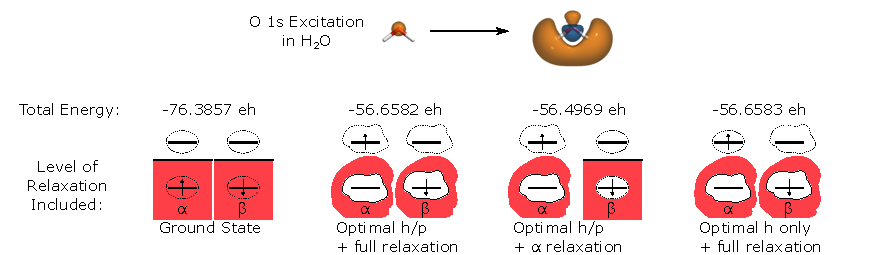
\includegraphics{h_p_algorithms.pdf}
\caption{First O 1s core excitation in H$_2$O calculated using orthogonality constrained density functional theory at the B3LYP/3-21G level of theory. Numbers reported are the total energy of the ground state and respective core excited state calculated with varying degrees of orbital relaxation included.}
\label{fig:relax}
\end{figure}
Figure \ref{fig:relax} shows the results of applying these different levels of relaxation to the first core excited state in H$_2$O. Optimizing the hole and particle pair with full relaxation yields a total energy of $- 56.6582$ Hartree. Only relaxing the $\alpha$ orbitals raises this energy by about 0.2 Hartree, showing that the rearangment that occurs in the electronic structure due to the creation of a core hole is significant. This highlights the importance of valence rearrangement and inclusion of hole relaxation effects. The ability of OCDFT to explicitly account for this effect makes it an excellent method for computing core-excitation energies accurately. 
\subsubsection{Stability of the Self-Consistent Algorithm}
The Ritz variational principle defines the energy expectation value $\tilde{E}$ of any trial wavefunction $\tilde{\phi}$ as an upper-bound with respect to the ground state energy $E_0$ of the system
\begin{equation}
\tilde{E} = \frac{\langle \tilde{\phi}| \hat{H} | \tilde{\phi}\rangle}{\langle\tilde{\phi}|\tilde{\phi}\rangle} \geq E_0.
\end{equation} 
However, the energy of a variationally computed excited state $E^{\prime}$ is no longer a valid upper bound of the ground state energy unless the trial wavefunction ($\tilde{\phi}$) is constrained to be orthogonal to all lower lying states of the same symmetry. In this regard, a standard $\Delta$SCF calculation of an excited state can be viewed as an unconstrained optimization, which in many cases guides the final optimized excited state solution to the ground state wave function. This is a well known optimization problem called ``variational collapse.'' Considering this issue, it is desirable to have a method that allows for the general variational calculation of an excited state without sacrificing the orthogonality of the computed excited state wavefunction to lower lying states of the same symmetry. Imposing orthogonality constraints into the variational procedure ensures the strict upperboundedness of the computed excited state energies, which ensures that the optimization will not suffer from variational collapse. This is the approach taken by orthogonality constrained density functional theory as well as the ``takes orthogonality constraints into account'' (TOCIA) method.\cite{tsaune_towards_1994} Other methods such as Morokuma's electron-hole potential (EHP) method\cite{morokuma_extended_1972} and the constricted variational DFT method (CV-DFT) of Ziegler et al. \cite{cullen_formulation_2011,ziegler_implementation_2012} aim to avoid this optimization problem without imposing exact orthogonality and instead impose different variational constraints. Despite these differences, all of these methods revolve around the variational minimization a unique KS energy functional for the excited state determinant $\Phi^{\prime}$ that is different from the ground state reference $\Phi$. They do this explicitly by parametrizing the wavefunction using a generic determinant, this can be expressed as a unitary transformation of the ground state determinant
\begin{equation}
|\Phi^{\prime} \rangle = |\phi_1^{\prime}, \phi_2^{\prime}, ..., \phi_n^{\prime} \rangle = e^{\hat{A}}|\Phi\rangle,
\end{equation}
where $\hat{A}$ is a one-particle anti-Hermitian operator. To impose an orthogonality condition on the excited state wavefunction ($\langle \Phi^{\prime}|\Phi\rangle$ = 0) OCDFT imposes the minimal orbital orthogonality constraints necessary to obtain an orthogonal solution. For example, to provide a description of the lowest excited state, the ground state HOMO ($\phi_n$) is simply constrained to be orthogonal to the excited state occupied orbitals ($\phi_i^{\prime}$) 
\begin{equation}
\langle \phi_n|\phi_i^{\prime} \rangle = 0, i = 1,2,...,n
\end{equation}
This constraint guarantees that the excited state determinant is orthogonal to the excited state, thus ensuring that the resulting optimization procedure does not suffer from variational collapse. 
\subsubsection{Favorable Computational Cost and Scaling}
A cheap computational cost and favorable scaling with respect to system size are extremely important features of OCDFT that allows for a wide range of potential applications for the method. Formally the cost of OCDFT is identical to that of a ground-state DFT computation which scales as $N^3$ for pure functionals and $N^4$ for hybrid functionals, where $N$ is the number of electrons in the system. This scaling with respect to system size is comparable to that of CIS and TDDFT which also scale as $N^4$, in which the bottleneck in those methods is the contraction of a transition density matrix with the two-electron integrals. This scaling is better than that of ADC(2) and excited state CC2 which scale as $N^5$. Unlike CIS and TDDFT, OCDFT maintains this favorable cost while still obtaining accurate excitation energies comparable to more expensive methods, as will be shown in Chapters 2 and 3 of this dissertation.
\section{Prospectus}
In Chapter 2, we report an extension of orthogonality constrained DFT to compute core excited states and generalize the original formalism in order to calculate multiple excited state solutions. This chapter focuses on benchmarking the method with respect to experimental core excitation energies and simulating full experimental spectra. Chapter 3 reports the combination of OCDFT with a novel implementation of the spin-free exact-two-component (X2C) one-electron treatment of scalar relatavistic effects in order to study the importance of relativistic effects on core-excited states and treat K-edges of transition metal complexes. Chapter 4 describes a new technique for the automated classification of core excited states that utilizes a unique representation of the unoccupied orbitals known as the localized intrinsic valence virtual orbitals (LIVVOs). This new method of classification is integrated with the OCDFT hole/particle orbital formalism here. Chapter 5 deals with the unique case of targeting the K-edge chemisorbed organic molecules. We introduce a subspace projection algorithm into OCDFT in order to specifically target the core excitations of the organic adsorbate, which is not feasible in the bottom-up algorithm described in Chapter 2.

{\footnotesize 
\bibliography{introduction}
\bibliographystyle{achemso}
}
\end{document}
\documentclass{article}
    % General document formatting
    \usepackage[margin=0.7in]{geometry}
    \usepackage[parfill]{parskip}
    \usepackage[utf8]{inputenc}
    \usepackage{graphicx}
    \usepackage[sort&compress,numbers,super]{natbib}
    \usepackage{booktabs}
    
    % Related to math
    \usepackage{amsmath,amssymb,amsfonts,amsthm}
    \graphicspath{{figures/}}
\begin{document}
\chapter{Simulation of X-Ray Absorption Spectra with Orthogonality Constrained Density Functional Theory}
\epigraph{\textit{``The history of science is rich in the example of the fruitfulness of bringing two sets of techniques, two sets of ideas, developed in separate contexts for the pursuit of new truth, into touch with one another.''}}{J. Robert Oppenheimer}
\begin{chapabstract}
Orthogonality constrained density functional theory (OCDFT) [F. A. Evangelista, P. Shushkov and J. C. Tully, \textit{J. Phys. Chem. A}, 2013, {\bf{117}}, 7378] is a variational time-independent approach for the computation of electronic excited states.
In this work we extend OCDFT  to compute core-excited states and generalize the original formalism to determine multiple excited states.
Benchmark computations on a set of 13 small molecules and 40 excited states show that \textit{unshifted} OCDFT/B3LYP excitation energies have a mean absolute error of 1.0 eV.
Contrary to time-dependent DFT, OCDFT excitation energies for first- and second-row elements are computed with near-uniform accuracy.
OCDFT core excitation energies are insensitive to the choice of the functional and the amount of Hartree--Fock exchange.
We show that OCDFT is a powerful tool for the assignment of X-ray absorption spectra of large molecules by simulating the gas-phase near-edge spectrum of adenine and thymine.
\end{chapabstract}

\section{Introduction}
The advent of synchrotron light sources created a strong resurgence of spectroscopy in the X-ray region. \cite{mcmillan_synchrotronproposed_1945} Near-edge X-ray absorption spectroscopy (NEXAS) is a useful experimental technique to probe the local electronic and geometrical structure in a variety of molecular environments.
The most dominant feature of NEXAS spectra, the \textit{near edge}  (see Fig.~\ref{fig:nexas-illustration}), is composed of the excitations of core-electrons to unoccupied valence orbitals.
Core excitations are atom-specific and sensitive to the local chemical environment, thus, NEXAS spectra can provide information about the chemical composition and the electronic structure of molecules.
NEXAS has been successfully applied to large biological systems, \cite{hua_refinement_2010} small molecules in the gas phase,\cite{contini_gas-phase_2001} organic thin-films,\cite{hahner_near_2006} and semiconducting materials.\cite{guo_electronic_2011} This wide range of applications is possible because synchrotron light sources can span an energy range that goes from a few electron volt (eV) \cite{feneberg_synchrotron-based_2011} to hundreds of MeV.\cite{nakazato_observation_1989}

\begin{figure}[!b]
\centering
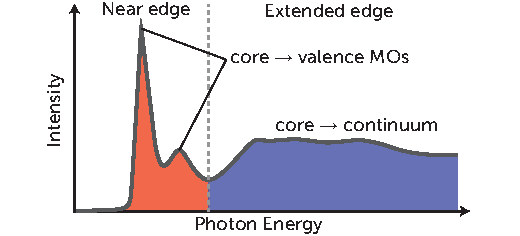
\includegraphics[width=8.8cm]{NEXASIllustration.pdf}
\caption{Example of a X-ray photoabsorption spectrum (XAS).  The near edge, located in the low energy region, consists of excitations of core electrons to valence orbitals.  These transitions are sensitive to the chemical environment surrounding the excited atom.  The high energy region of the spectrum results from excitations of core electrons to the continuum.}
\label{fig:nexas-illustration}
\end{figure}

As NEXAS experiments are becoming more feasible, there is a growing need to develop accurate theoretical approaches to aid the interpretation of experimental spectra.
%In order for a method to properly replicate and analyze NEXAS spectra, it must demonstrate accuracy in describing core-electron excitations. 
Calculations of NEXAS spectra are challenging, and require computational methods that explicitly account for the excitations of core-level electrons, orbital relaxation effects, and electron correlation. \cite{coriani_coupled-cluster_2012} Several theoretical approaches have been adapted to compute core-valence excitations, including: scaled-opposite-spin configuration interaction singles with perturbative doubles [SOS-CIS(D)],\cite{asmuruf_calculation_2008} a restricted open-shell DFT/CIS method,\cite{roemelt_excited_2013,roemelt_combined_2013} second-order algebraic digrammatic construction [ADC(2)],\cite{schirmer_beyond_1982,trofimov_efficient_1995} multiple scattering X$_\alpha$ methods, \cite{sheehy_correlation_1989} a maximum overlap $\Delta$SCF approach, \cite{besley_self-consistent-field_2009} restricted active space SCF method (RASSCF), \cite{agren_relaxation_1993} transition potential theory,\cite{triguero_calculations_1998} coupled-cluster response theory, \cite{coriani_coupled-cluster_2012} time-dependent density functional theory (TDDFT),\cite{stener_time_2003} and restricted excitation window TDDFT (REW-TDDFT). \cite{lopata_linear-response_2012} Among these methods, TDDFT is perhaps the most attractive option because of its reduced computational cost and ability to calculate multiple excited states.

TDDFT is a rigorous extension of the DFT ground-state formalism,\cite{runge_density-functional_1984} and it is regarded as the method of choice to treat electronic excited states within a density functional framework.
%Within the framework of density functional theory, TDDFT is regarded as the method of choice to treat electronic excited states because it is a rigorous extension of the ground-state formalism.\cite{runge_density-functional_1984}
 When applied in conjunction with frequency-independent exchange-correlation potentials, TDDFT yields accurate excitation energies for low-lying excited states. For example, the TDDFT benchmark study of Silva-Junior and co-workers\cite{silva-junior_benchmarks_2008} on 28 organic molecules, showed that singlet and triplet excitation energies can be calculated with a mean average error (MAE) of 0.27 eV and 0.44 eV, respectively. However, Besley et al.\cite{besley_self-consistent-field_2009} showed that TDDFT core excitations computed with conventional exchange-correlation functionals grossly underestimate experimental results, yielding a MAE of 20.2 eV. It is customary to remedy this deficiency of TDDFT by shifting the position of computed spectra by an amount that minimizes the difference between the computational and experimental peak features. For example, a study done by DeBeer, Petrenko, and Neese\cite{debeer_george_prediction_2008} showed that it is necessary shift the TDDFT Fe near-edge spectrum of different iron complexes by 171.3 eV in order to achieve quantitative agreement with experiment. This shift is dependent on the basis set and functional used and must be recalibrated for every basis set/functional combination applied to a given system.

Work by Peach et al.\cite{peach_excitation_2008} provided evidence for a direct correlation between the accuracy of TDDFT and the degree of spatial overlap ($\Lambda$) between the occupied and virtual orbitals.
The inaccuracy of TDDFT for excitations with low values of $\Lambda$ has been attributed to the incorrect asymptotic behavior of the exchange-correlation potential and self-interaction error.\cite{peach_excitation_2008} Low orbital overlap is a characteristic feature of both charge-transfer excitations and core excitations, and as expected, the same correlation between accuracy and orbital overlap is observed for core excitations.\cite{besley_time-dependent_2009}
As a consequence, TDDFT core-valence excitation energies can be improved by introducing self-interaction corrections (SIC)\cite{tu_core_2007} or range separated hybrid functionals in which the amount of long and short range Hartree--Fock exchange is reparametrized.\cite{besley_time-dependent_2009, nakata_time-dependent_2006}  However, the optimal value of the range separation parameter and the amount of Hartree--Fock exchange are strongly system dependent and must be tuned.\cite{capano_role_2013,besley_time-dependent_2007,besley_time-dependent_2010}
%Given the difficulties encountered by TDDFT in computing charge-transfer excited states\cite{dreuw_failure_2004} and the self interaction error that afflicts traditional density functionals, this failure is to be expected.


A general method that can systematically produce accurate core-excitation energies with traditional (that is, non range corrected) hybrid density functionals is highly desirable. The maximum overlap method (MOM) \cite{besley_self-consistent-field_2009} combined with a $\Delta$SCF treatment of core-valence excitations is able to obtain highly accurate excitation energies using conventional functionals. However, this procedure is not guaranteed to avoid the problem of variational collapse---albeit MOM ameliorates the difficulties encountered by a straightforward $\Delta$SCF procedure---and has not been generalized to multiple excited states of the same symmetry.

The goal of this work is to find cost-effective alternative theories to TDDFT that can be used to simulate NEXAS spectra.
Orthogonality constrained density functional theory (OCDFT)\cite{evangelista_orthogonality_2013}  was rigorously derived from a variational time-independent formulation of excited state DFT.
It builds upon previous successful efforts to formulate variational excited state DFT, such as: the $\Delta$SCF procedure, \cite{kowalczyk_assessment_2011,ziegler_calculation_1977} constrained DFT,\cite{wu_constrained_2006} stationary state DFT, \cite{gorling_density-functional_1999}  constricted variational density functional theory (CV-DFT), \cite{ziegler_relation_2009,ziegler_application_2011,krykunov_self-consistent_2013,ziegler_implementation_2012}
perturbative constrained excited state DFT,\cite{baruah_dft_2009,olguin_effect_2013,zope_charge_2012} ensemble DFT,\cite{theophilou_energy_1979,fritsche_generalized_1986,gross_rayleigh-ritz_1988,gross_density-functional_1988} and variational time independent DFT (TI-DFT). \cite{levy_variational_1999,nagy_variational_2001}
Formally, OCDFT may be viewed as bridging constrained and constricted variational DFT.  Its main advantages are: 1) a favorable accuracy/cost ratio, similar to that of ground state DFT, 2) a numerically robust optimization procedure that avoids variational collapse, and 3) the ability to compute spin adapted excitation energies.
Benchmark computations\cite{evangelista_orthogonality_2013} show that valence excitation energies computed with OCDFT have error metrics comparable to that of TDDFT.  In addition, OCDFT has the ability to accurately compute charge-transfer excitation energies regardless of the amount of Hartree--Fock exchange present in the exchange-correlation functional.

This work introduces two new developments of OCDFT that are necessary for the simulation of near-edge X-ray  absorption spectra.
First, we formulate an OCDFT algorithm that can be used to compute core-valence excitation energies.  This new method is assessed over a test set that includes 13 molecules with 40 unique core-electron excitations.
Second, we discuss one approach to extend OCDFT to multiple excited states of the same symmetry.
We demonstrate the potential of this new method with computations of the gas-phase near-edge spectrum of adenine and thymine.


\section{Theory}
In this section we provide a brief summary of orthogonality constrained density functional theory along with the necessary extension to multiple excited states (for the full details of the OCDFT derivation we refer the reader to Ref.\citenum{evangelista_orthogonality_2013}).
OCDFT builds upon the time-independent variational DFT approach developed by Ayers, Levy, and Nagy.\cite{ayers_time-independent_2012}
Within this framework, each electronic state ($\Psi^{(n)}, n=0,1,\ldots$) of a $N$-electron system has a corresponding density functional ($E^{(n)}[\rho]$) which is a generalization of the ground-state functional of Levy.   $E^{(n)}[\rho]$ minimizes the energy expectation value $\bra{\Psi}\hat{H}\ket{\Psi}$ imposing two constraints on to the trial wave function $\Psi$: 1) $\Psi$ must be compatible with the density $\rho$, and 2) $\Psi$ must be orthogonal to the first $n-1$ \textit{exact} electronic states, $\{\Psi^{(k)}, k = 1,\ldots,n-1\}$:
\begin{equation}
E^{(n)}[\rho] = \min_{
\substack{
\Psi \rightarrow \rho\\
\Psi\bot \{\Psi^{(k)}\}
}
}
\bra{\Psi}\hat{H}\ket{\Psi}.
\end{equation}

OCDFT provides a practical realization of this time-independent DFT approach.
The first step in the OCDFT derivation consists in defining a generalized Kohn--Sham scheme that, for each electronic state $\Psi^{(n)}$,  postulates an auxiliary system of noninteracting electrons with wave function $\Phi^{(n)}$ and density $\rho_s^{(n)}$.  The density of state $\Phi^{(n)}$ is assumed to be equal to the density of the exact state $\Psi^{(n)}$, which we indicate with $\rho^{(n)}$.
In addition, we assume that the auxiliary wave functions are orthogonal, that is:
\begin{equation}\label{eq:orthogonality_condition}
\braket[1]{\Phi^{(m)}}{\Phi^{(n)}} = \delta_{mn}.
\end{equation}
This condition can be imposed without loss of generality.  It avoids the excited state wave functions from collapsing down to the ground state solution, and effectively transfers some of the complexity of the excited state density functionals to the kinetic energy operator.
Nevertheless, this variational Kohn--Sham scheme involves energy functionals [$E_{\rm KS}^{(n)}$] that contain exchange-correlation contributions [$E^{(n)}_{\rm xc}$] \textit{specific} for each excited state.
In OCDFT, we invoke an adiabatic approximation similar to the one used in TDDFT, and replace $E^{(n)}_{\rm xc}$ with the ground state exchange-correlation functional, $E^{(0)}_{\rm xc}$.
The resulting functional for excited state $n$ is given by:
\begin{equation}
\begin{split}\label{eq:OCDFTfunctional}
E^{(n)}_{\rm OCDFT}[\{\phi^{(n)}_i\}]=& -\frac{1}{2} \sum_i^{\rm occ} \bra[1]{\phi_i^{(n)}}\nabla^2\ket[1]{\phi_i^{(n)}} + 
\int d \mathbf{r} \, v(\mathbf{r}) \rho^{(n)}(\mathbf{r})\\
 &+ J[\rho^{(n)}] + E^{(0)}_{\rm xc}[\rho^{(n)}]. 
\end{split}
\end{equation}

\begin{figure}
\centering
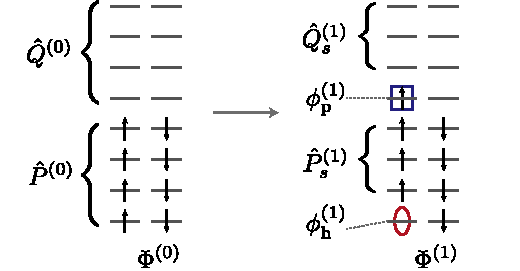
\includegraphics[width=8.8cm]{Figure1.pdf}
\caption{Illustration of the projection operators used in OCDFT.
%the ground state determinant $\Phi^{(0)}$ and the excited state determinant $\Phi^{(1)}$.
Notice, that a consequence of Eqs.~\eqref{eq:pq_conditions1}--\eqref{eq:pq_conditions2} is that the hole [$\phi^{(1)}_{\rm h}$] and particle [$\phi^{(1)}_{\rm p}$] orbitals are contained in the spaces spanned by $\hat{P}^{(0)}$ and $\hat{Q}^{(0)}$.}
\label{fig:projection}
\end{figure}
Minimization of the $E^{(n)}[\{\phi^{(n)}_i\}]$ with respect to the occupied orbitals for state $n$ can be performed with a modified self-consistent-field algorithm.\cite{evangelista_orthogonality_2013}
In the case of the first excited ($n = 1$), it is possible to show that the orthogonality condition [Eq.~\eqref{eq:orthogonality_condition}] implies the existence of two special orbitals.
As illustrated in Fig.~\ref{fig:projection}, these are the \textit{hole} [$\phi^{(1)}_{\rm h}$] and \textit{particle} [$\phi^{(1)}_{\rm p}$] orbitals, which are respectively unoccupied and occupied in the excited state wave function $\Phi^{(1)}$.
These orbitals must satisfy the conditions:
\begin{align}
\label{eq:pq_conditions1}
\hat{Q}^{(0)}\phi_{\rm h}^{(1)} = 0,\\
\label{eq:pq_conditions2}
\hat{P}^{(0)}\phi_{\rm p}^{(1)} = 0,
\end{align}
where $\hat{P}^{(0)} = \sum_{i} \ket[1]{\phi_i^{(0)}}\bra[1]{\phi_i^{(0)}}$ is a projector onto the occupied orbitals of $\Phi^{(0)}$, and $\hat{Q}^{(0)} = 1 - \hat{P}^{(0)}$.
Eqs.~\eqref{eq:pq_conditions1} and \eqref{eq:pq_conditions2} can be enforced via Lagrangian multipliers.
Setting the variation of the Lagrangian with respect to the occupied ($\{\phi^{(1)}_i\}$), hole ($\phi^{(1)}_{\rm h}$), and particle ($\phi^{(1)}_{\rm p}$) orbitals to zero gives the following eigenvalue equations:
\begin{align}
\label{eq:one_state_occ_eq}
(1 - \hat{P}^{(1)}_{\rm h/p})\hat{f}^{(1)} (1 - \hat{P}^{(1)}_{\rm h/p})|\phi_i^{(1)}\rangle &= \epsilon^{(1)}_i |\phi_i^{(1)}\rangle,\\
\label{eq:one_state_hole_eq}
\hat{P}^{(0)}(1-\hat{Q}_{\rm s}^{(1)}) \hat{f}^{(1)} (1-\hat{Q}_{\rm s}^{(1)})\hat{P}^{(0)} |\phi_{\rm h}^{(1)}\rangle &= \epsilon^{(1)}_{\rm h} |\phi_{\rm h}^{(1)}\rangle,\\
\label{eq:one_state_part_eq}
\hat{Q}^{(0)}(1-\hat{P}_{\rm s}^{(1)}) \hat{f}^{(1)} (1-\hat{P}_{\rm s}^{(1)}) \hat{Q}^{(0)}|\phi_{\rm p}^{(1)}\rangle &= \epsilon^{(1)}_{\rm p} |\phi_{\rm p}^{(1)}\rangle,
\end{align}
where $\hat{f}^{(1)} $ is the Kohn--Sham Hamiltonian of the excited state.
Eq.~\eqref{eq:one_state_occ_eq} determines the occupied orbitals, while Eqs.~\eqref{eq:one_state_hole_eq} and \eqref{eq:one_state_part_eq} determine the hole and particle orbitals, respectively.
The projection operators involved in the OCDFT equations are defined as (see Fig.~\ref{fig:projection}):
\begin{align}
\hat{P}^{(1)}_{\rm h/p} &= \hat{P}^{(1)}_{\rm h} + \hat{P}^{(1)}_{\rm p} = 
\ket[1]{\phi^{(1)}_{\rm h}}\bra[1]{\phi^{(1)}_{\rm h}}
+\ket[1]{\phi^{(1)}_{\rm p}}\bra[1]{\phi^{(1)}_{\rm p}},\\
\hat{P}^{(1)}_{\rm s} &= \hat{P}^{(1)} - \hat{P}^{(1)}_{\rm p},\\
\hat{Q}^{(1)}_{\rm s} &= \hat{Q}^{(1)} - \hat{P}^{(1)}_{\rm h},
\end{align}
where the subscript ``s'' stands for \textit{spectator} orbitals.
%See Fig.~\ref{fig:projection} for a graphical representation of the projection operators.
In OCDFT computations of valence excited states, the hole orbital is assumed to be the solution of Eq.~\eqref{eq:one_state_hole_eq} with the highest value of $\epsilon^{(1)}_{\rm h}$.  Similarly, the particle orbital corresponds to the lowest eigenvalue of Eq.~\eqref{eq:one_state_part_eq}.

\begin{figure*}
\centering
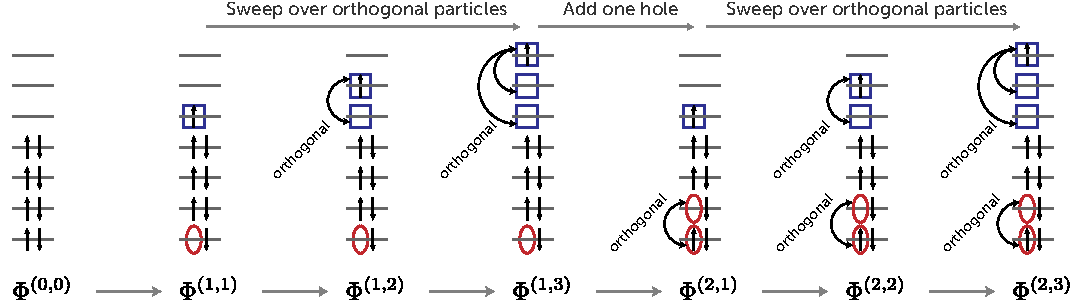
\includegraphics[width=15.5cm]{Figure2NEW.pdf}
\caption{Constrained multiple hole/particle (CMHP) algorithm illustrated in the case of two hole and three particle orbitals.}
\label{fig:CMHP}
\end{figure*}
Our OCDFT approach for core-excited states introduces two new aspects.
First, in order to compute core-excited states with OCDFT, we select hole orbitals with the smallest values of $\epsilon^{(1)}_{\rm h}$.
However, this simple extension allows us only to compute one core-excited state for each irreducible representation.
In principle, OCDFT can be generalized to compute an arbitrary number of excited states.  For each additional excited state, it is necessary to minimize the OCDFT energy imposing orthogonality with respect to the lower energy solutions.
While this appears to be a viable solution, it would undoubtedly lead to a more elaborate minimization procedure.
In this work we propose simplified orthogonality conditions that are based on the orthogonality of the hole and/or particle orbitals.
For example, if we choose the hole orbital for the second excited state [$\phi_{\rm h}^{(2)}$] to be orthogonal to the first hole [$\phi_{\rm h}^{(1)}$] and to spans the occupied space of the ground state determinant:
\begin{align}
\label{eq:ortho_example_1}
\braket[1]{\phi_{\rm h}^{(2)}}{\phi_{\rm h}^{(1)}} = 0,\\
\label{eq:ortho_example_2}
\hat{Q}^{(0)}\phi_{\rm h}^{(2)} = 0,
\end{align}
then the determinant $\Phi^{(2)}$ is guaranteed to be orthogonal to $\Phi^{(0)}$ and $\Phi^{(1)}$.
The conditions Eqs.~\eqref{eq:ortho_example_1} and \eqref{eq:ortho_example_2} are sufficient but not necessary to guarantee orthogonality among the first three electronic states. 

In the following we describe our constrained multiple hole/particle (CMHP) algorithm, which generalizes Eqs.~\eqref{eq:ortho_example_1} and \eqref{eq:ortho_example_2} to the case of $n$ electronic states.  Due to the complexity of this algorithm, we recommend the reader to follow its description with the help of Fig.~\ref{fig:CMHP}.
Suppose we are interested in the excited states that result from the excitation of a given number of core orbitals ($n_{\rm c}$) and unoccupied orbitals ($n_{\rm u}$).
For convenience we will label the excited state Kohn--Sham determinants [$\Phi^{(i,a)}$] with two indices, $i$ and $a$, which stand respectively for the core and unoccupied orbital that are involved in an excited state.
Our algorithm starts with a ground-state DFT computation, which yields the determinant $\Phi^{(0,0)}$.
Next, we perform a sweep of $n_{\rm u}$ OCDFT computations, which produces the series of solutions:
\begin{equation}
\Phi^{(1,1)}, \Phi^{(1,2)}, \ldots, \Phi^{(1,n_{\rm u})}.
\end{equation}
These solutions are characterized by hole (particle) orbitals that span the occupied (unoccupied) space of $\Phi^{(0,0)}$:
\begin{align}
\begin{cases}
\hat{Q}^{(0)}\phi_{\rm h}^{(1,a)}= 0\\
\hat{P}^{(0)}\phi_{\rm p}^{(1,a)}= 0
\end{cases} &,&\forall a \leq n_{\rm u},
\end{align}
and particle orbitals that form an orthogonal set:
\begin{align}
\braket[1]{\phi^{(1,a)}_{\rm p}}{\phi^{(1,b)}_{\rm p}} &= \delta_{ab}, &\forall a,b \leq n_{\rm u}.
\end{align}


In the following iteration of the CMHP algorithm we increase the core index by one and sweep again through a series of solutions:
\begin{equation}
\Phi^{(2,1)}, \Phi^{(2,2)}, \ldots, \Phi^{(2,n_{\rm u})},
\end{equation}
such that the hole and particle orbitals span respectively the virtual and occupied space of the ground-state determinant:
\begin{align}
\begin{cases}
\hat{Q}^{(0)}\phi_{\rm h}^{(2,a)}= 0\\
\hat{P}^{(0)}\phi_{\rm p}^{(2,a)}= 0
\end{cases} &,&\forall a \leq n_{\rm u},
\end{align}
and the particle orbitals are orthogonal:
\begin{align}
\braket[1]{\phi^{(2,a)}_{\rm p}}{\phi^{(2,b)}_{\rm p}} &= \delta_{ab},&\forall a,b \leq n_{\rm u}.
\end{align}
In addition, we impose orthogonality between the first core orbital of the first sweep, $\phi^{(1,1)}_{\rm h}$, and the second core orbital of each of the states determined during the current sweep, $\phi^{(2,a)}_{\rm h}$:
\begin{align}
\braket[1]{\phi^{(1,1)}_{\rm h}}{\phi^{(2,a)}_{\rm h}} &=0,&\forall a \leq n_{\rm u}.
\end{align}
This condition guarantees that the hole orbital for the second series of computations is different from the first one.
The CMHP algorithm proceeds in a similar way until $i = n_{\rm c}$.  After each sweep over the particle orbitals, a new set of orthogonality conditions is imposed onto the hole orbitals.
We notice that the CMHP algorithm does \textit{preserve strict orthogonality among all states}, but it is not equivalent to imposing the strictly minimum orthogonality conditions.

In summary, the CMHP algorithm simplifies the optimization of a series of mutually orthogonal determinants by imposing separate orthogonality conditions onto the core (hole) and valence (particle) orbitals.
It is instructive to compare the computational cost of OCDFT and TDDFT.
The cost to compute $d$ excited state in OCDFT is proportional to $d N^3$ and $d N^4$ for pure and hybrid functional, respectively, since for each excited states one has to solve a set of constrained Kohn--Sham equations.
In the case of TDDFT, the computational cost is dominated by the solution of a pseudo-eigenvalue problem, which scales as $d N^4$.
TDDFT certainly provides a more direct approach to the computation of multiple excited states, but in our experience we observe that the OCDFT/CMHP algorithm has a cost comparable to that of TDDFT and in most cases can be applied in a black-box way.


\section{Computational Details}
Our OCDFT for core-excited states was implemented as a plugin for the \textsc{psi4} \textit{ab initio} quantum chemistry package.\cite{turney_psi4:_2012}
The OCDFT excitation energies for a set of 13 small molecules reported in this study were computed using the B3LYP, \cite{becke_new_1993,lee_development_1988,vosko_accurate_1980,stephens_ab_1994} PBE0 \cite{adamo_toward_1999}, and BLYP\cite{stephens_ab_1994,miehlich_results_1989} functionals, using the correlation-consistent polarized core-valence basis sets (cc-pCV$X$Z, $X$ = T,Q)\cite{woon_gaussian_1995-1}
and the Karlsruhe valence polarized basis sets (def2-$X$ZVP, $X$ = T,Q).\cite{weigend_balanced_2005,weigend_accurate_2006} All geometries were optimized at the same level of theory as the given excitation energy.
The optimized geometries and the NEXAS spectrum of adenine and thymine were computed at the def2-TZVP/B3LYP level of theory (cartesian geometries are provided in the supplementary material).
Benchmark TDDFT excitation energies were computed at the B3LYP/def2-QZVP level of theory using the ORCA software package.\cite{neese_orca_2012}
All excitation energies reported in this work, including TDDFT, are for singlet states.
In the case of OCDFT, the singlet excitation energies were computed via the spin-raising approach described in Ref.~\citenum{evangelista_orthogonality_2013}.


It is mandatory to consider relativistic effects when studying excitations of core electrons.\cite{maganas_l-edge_2014,debeer_george_calibration_2010,bauer_herfd-xas_2014,ankudinov_sensitivity_2002}
%Work by Desclaux et al. \cite{desclaux_relativistic_1971} shows that the largest orbital effect when solving the relativistic hartree-fock equations is the contraction of the 1s orbital, the corresponding energy correction ($\Delta\epsilon_{\text{1s}}$) can be approximated by 
For excitations involving 1s orbitals, we approximate the relativistic excitation energy ($\omega^{\rm R}$) as the sum of the nonrelativistic excitation energy ($ \omega^{\rm NR}$) minus a correction $\Delta\epsilon_{\text{1s}}$:
\begin{align}
\omega^{\rm R} = \omega^{\rm NR} - \Delta\epsilon_{\text{1s}} ,
\end{align}
where $\Delta\epsilon_{\text{1s}}$ is the energy difference between the ground-state nonrelativistic (NR) and relativistic (R) Kohn--Sham energies of the 1s orbital:
\begin{align}
\Delta\epsilon_{\text{1s}} = \epsilon_{\text{1s}}^{\text{R}} - \epsilon_{\text{1s}}^{\text{NR}}.
\end{align}
In this work, the excitation energies computed in OCDFT and TDDFT utilize relativistic orbital energies calculated with first-order Douglass--Kroll--Hess (DKH) Hamiltonian.\cite{douglas_quantum_1973,hess_applicability_1985, hess_relativistic_1986} 
Relativistic corrections for the 1s orbitals of the second row nuclei range from 3.8 eV (Si) to 10.1 eV (Cl). 
In the case of first row 1s core orbitals, $\Delta\epsilon_{\text{1s}}$ is negligible (C, N, and O 1s corrections are about 0.1, 0.2, and 0.3 eV, respectively).  Similarly, excitations from 2p orbitals of second row elements are negligible (max 0.05 eV) and were not applied to the final results.

The treatment of core-excited states in molecules with symmetry equivalent atoms becomes problematic for both pure and hybrid functionals due to the approximate treatment of exchange and correlation which introduces a self-interaction error.\cite{bally_incorrect_1997,lundberg_quantifying_2005} In this case, the symmetry restricted solution produces core holes distributed evenly amongst the symmetry equivalent atoms. 
Instead, the symmetry unrestricted solution may consists of core holes localized on  each individual atom. 
For all molecules with symmetry equivalent atoms (N$_2$, C$_2$H$_2$, and Cl$_2$) we studied both the symmetry restricted and unrestricted solutions.
To obtain a state where the core hole is localized, we utilize a wave function with broken spatial and spin symmetry mixing the coefficients of the alpha and beta orbitals.

Peak intensities for the transition $\Psi^{(n)} \leftarrow \Psi^{(0)}$ are based on the oscillator strength ($f_{\rm osc} $):
  \begin{align}
  \label{osc}
  f_{\rm osc} = \frac{2}{3} |\mu_{n0}|^2 \omega_{n},
  \end{align}
which is calculated from the excitation energies ($\omega_{n}$) and transition dipole moments ($\boldsymbol{\mu}_{n0}$).
Although OCDFT does not provide a direct way to compute transition dipole moments, these can be approximated using the Kohn--Sham determinants as:
\begin{equation}
\boldsymbol{\mu}_{n0} = \bra[1]{\Phi^{(n)}} \hat{\textbf{r}}\ket[1]{\Phi^{(0)}},
\end{equation}
where $\Phi^{(n)}$ is a generic excited state and $\hat{\textbf{r}}$ is the position vector.
Eq.~\eqref{osc} yields the absolute oscillator strength ($f_{\rm abs}$) for a given transition. The intensity of the spectrum is then scaled relative to the most intense peak, we will refer to these scaled values as the \textit{relative oscillator strength} ($f_{\rm rel}$).
Natural spectroscopic broadening effects are simulated by convoluting the OCDFT peaks with a Gaussian function whose exponent was calibrated to best fit the experimental spectrum.
%This procedure yield Gaussian widths in the range 0.1--0.4 eV.

\section{Results and Discussion}
%OCDFT was used to compute 40 unique core-excitations from a test set of 13 molecules. Its accuracy was assessed by comparing it to experimental data from gas-phase NEXAS experiments.\cite{puttner_vibrationally_1999,remmers_high-resolution_1992,chen_k-shell_1989,tronc_nitrogen_1980,tronc_carbon_1979,francis_studies_1994,adachi_vibronic_1999,hitchcock_k-shell_1979,domke_carbon_1990,nayandin_angle-resolved_2001,bodeur_single-and_1990} 
%Excitations from 1s orbitals are considered for all multi-electron atoms in each molecule, in addition to excitations from 2p orbitals for second row elements. 
%The MAEs of OCDFT over the test set are shown in Table \ref{table:OverallPerformance}, considering 12 unique basis set and functional combinations. A direct comparison of the accuracy of OCDFT and TDDFT compared to experimental core-excitation energies are shown in Figure \ref{figure:Hist}. A breakdown of individual excitations computed with OCDFT and TDDFT are compared to their experimental assignments in Tables \ref{table:FirstRow} and \ref{table:SecondRow}. Table \ref{table:FirstRow} displays excitations from first row atoms, while Table \ref{table:SecondRow} shows excitations from second row atoms. We observe a distinct relationship between the amount of hole/particle orbital overlap and the accuracy of the computations, this relationship is explained in Section 4.3 and further analyzed in Figure \ref{figure:scatter}. Finally we close by computing the NEXAS spectra of two nucleobases, adenine and thymine. The nitrgen, carbon, and oxygen edges for Thymine can be found in Figure \ref{figure:Thymine} while the carbon and nitrogen edges of Adenine are found in Figure \ref{figure:Adenine}. Spectra resulting from inner-shell ionizations are commonly referred to as K, L, or M edges depending on which core-shell is involved in the excitation. This nomenclature is simply derived from the Barkla labeling scheme for X-ray series, and we will routinely employ it to refer to specific spectra.
\subsection{Calibration of OCDFT core-excitation energies}
\begin{table}[!b]
\small
\caption{OCDFT core-excitation energies for a benchmark set composed of 13 diatomic molecules.  Mean absolute error (in eV) computed using various combinations of basis sets and density functionals. These statistics refer to a subset of the benchmark set comprised of 35 core-excited states.}
\centering
    \begin{tabular}{lccc}
    \hline
    \hline
Basis Set & \multicolumn{3}{c}{Mean Absolute Error (eV)}  \\
& BLYP & B3LYP & PBE0\\
\hline
def2-TZVP & 1.0 & 1.0 & 0.9 \\
def2-QZVP & 1.0 & 1.0 & 1.4 \\
cc-pCVTZ & 1.3 & 1.3 & 1.6 \\
cc-pCVQZ & 1.5 & 1.5 & 1.7 \\
\hline
\hline
\end{tabular}
\label{table:OverallPerformance}
\end{table}
The accuracy of OCDFT was benchmarked using a test set that comprises molecules containing first-row (CO, H$_2$CO, N$_2$O, N$_2$, HCN, CH$_4$, C$_2$H$_4$) and second-row elements (SiH$_4$, PH$_3$, H$_2$S, SO$_2$, HCl, Cl$_2$), and a total of 40 excited states. 
Table \ref{table:OverallPerformance} summarizes the performance of OCDFT by reporting the mean absolute error (MAE) in the excitation energy for 12 unique combinations of basis set and density functionals.
Individual excitation energies computed with OCDFT and TDDFT are compared to values from gas-phase NEXAS experiments \cite{puttner_vibrationally_1999,remmers_high-resolution_1992,chen_k-shell_1989,tronc_nitrogen_1980,tronc_carbon_1979,francis_studies_1994,adachi_vibronic_1999,hitchcock_k-shell_1979,domke_carbon_1990,nayandin_angle-resolved_2001,bodeur_single-and_1990,gedat_s_1998,hudson_high-resolution_1994,cavell_chemical_1999,bodeur_photoabsorption_1985} in Tables \ref{table:FirstRow} and \ref{table:SecondRow}. Table \ref{table:FirstRow} displays excitations from first-row elements, while Table \ref{table:SecondRow} shows excitations from second-row elements. For molecules with symmetry-equivalent atoms (N$_2$, C$_2$H$_2$, and Cl$_2$), we examined both the symmetrical and symmetry-broken solutions and found that the former have a MAE of 13.7 eV, while the latter yield a MAE of 0.9 eV.
Thus all results for highly symmetric molecules reported in Tables~\ref{table:FirstRow} and \ref{table:SecondRow} are based on broken symmetry solutions.
\begin{figure}[!h]
\centering
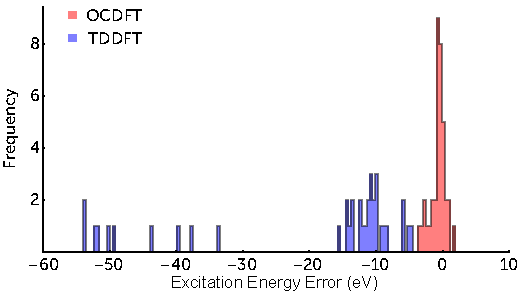
\includegraphics[width=8.8cm]{NEW_histogram2.pdf}
\caption{Histogram showing the distribution of the error in the computed core excited states. All calculations were done using the B3LYP functional and the def2-QZVP basis set. The red filled bar is OCDFT while the empty blue bar is TDDFT. Notice that the two distributions do not overlap.}
\label{figure:Hist}
\end{figure}
The three functionals considered in Table~\ref{table:OverallPerformance} produce MAEs ranging from 0.9--1.7 eV. Interestingly, there is no dramatic difference in the accuracy of OCDFT regardless of the amount of Hartree--Fock (HF) exchange present in the functional. Even the BLYP functional, which contains no HF exchange, yields a MAE (1.0 eV using the def2-QZVP basis set) comparable to that of the MAEs produced by its hybrid counterparts.
%B3LYP produces errors in the range of 1.0 eV $\rightarrow$ 1.5 eV, while PBE0 produces errors in the range of 0.9 eV $\rightarrow$ 1.7 eV. BLYP outperforms PBE0 when employing three of the fours basis sets considered and yields similar MAEs as B3LYP.
The Karlsruhe family of basis sets yields results that are in better agreement with the experimental excitation energies than the correlation-consistent basis sets.

The average error of OCDFT is commensurate to that of wave function methods for core-excited states. For example, Asmuruf and Besley\cite{asmuruf_calculation_2008} reported an average error of 1.2 eV for SOS-CIS(D) applied to a set of excitations similar to the ones used in the present study. While Coriani et al.\cite{coriani_coupled-cluster_2012} reported absolute errors of less than 0.9 eV when applying coupled cluster response theory to a set of carbon, nitrogen, and neon core excitations. 

A full comparison of the accuracy of OCDFT and TDDFT core-excitations computed at the B3LYP/def2-QZVP level of theory is shown in Fig. \ref{figure:Hist}.
The contrast between the two error distributions is striking.  As expected, TDDFT performs rather poorly underestimating the excitation energies, on average, by 15 eV and a maximum error of $-$53.6 eV. 
On the contrary, OCDFT yields an error distribution peaked near zero and a maximum error of $-$3.7 eV.
The TDDFT error distribution has a peculiar shape, displaying two distinct groups of excited states. The first is a narrow distribution that exists in the range $-$4 eV to $-$15 eV, while the second one is broader and ranges from $-$54 eV to $-$38 eV. An analysis of the group of excited states with the largest errors reveals that these consist solely of 1s core-excitations of second-row elements. This finding is in agreement with previous studies by Nakata \cite{nakata_extension_2007} and Besley. \cite{besley_time-dependent_2009} Since our excitation energies are corrected for relativistic effects (albeit with a crude approximation), the bulk of the error observed for second-row elements must be attributed to a deficiency of the exchange-correlation functional.\cite{saue_relativistic_2011} This dramatic difference in the performance of TDDFT suggests that it is helpful to separately analyze first-row and second-row core excitations to highlight their distinctive features.
%A common source of error in the calculation of core excited states is the inadequate treatment of relativistic effects. It is crucial that we reiterate that all excitation energies were computed using the DKH relativistic Hamiltonian, thus this eliminates relativistic effects as a potential source of error for TDDFT.\cite{saue_relativistic_2011}

%Fig. \ref{figure:Hist} hints at a specific difficulty of conventional TDDFT. Notice the gap, roughly 15 eV wide, that exists between the two clusters of TDDFT data. This gap exists because TDDFT becomes sharply more inaccurate when dealing with second row core excitations \cite{nakata_extension_2007,besley_time-dependent_2009}. 
%All of the TDDFT excitation energies that have an absolute error greater than 20 eV can be attributed to core excitations involving 1s orbitals located on second row nuclei. 
\begin{figure}[!b]
\centering
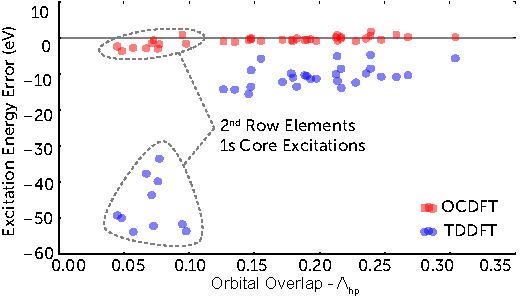
\includegraphics[width=8.8cm]{scatterNEWER2.pdf}
\caption{Scatterplot displaying the excitation energy error as a function of orbital overlap for a benchmarking test set of 40 core excitations from 13 different molecules. Excitation energies were calculated using the B3LYP functional and def2-QZVP basis set. The overlap integrals were computed with numerical grid integration making use of the Gaussian cube files produced by in Psi4 OCDFT calculations. Grids were calculated with a double zeta basis set and 0.1 grid spacing.}
\label{figure:scatter}
\end{figure}
Table \ref{table:FirstRow} reports valence and Rydberg excitation energies of 1s orbital localized on first row elements (C, N, or O). Compared to experiment, TDDFT produces a mean absolute error of 11.6 eV, and as discussed earlier, this result is consistent with previous studies that used TDDFT with conventional hybrid functionals.\cite{besley_self-consistent-field_2009} OCDFT calculations yield a mean absolute error of 0.4 eV. To put this error into perspective, it can be compared to the performance of TDDFT with the BH$^{0.58}$LYP functional,\cite{besley_time-dependent_2009} a reparameterization of the BHLYP functional\cite{becke_new_1993,lee_development_1988-1} that has been augmented to include 58\% HF exchange, 39\% B88 exchange, and 8\% Slater exchange. When applied to a test set of first row core excitations similar to those in Figure \ref{table:FirstRow}, BH$^{0.58}$LYP yielded a mean average error of 0.8 eV. It is encouraging that OCDFT can achieve a higher level of accuracy without altering the amount of Hartree--Fock exchange included in the functional. It is also gratifying to see that the OCDFT MAE for this set of first row core excited states is comparable to the MAE obtained for valence excited states (0.3 eV reported in Ref. \citenum{evangelista_orthogonality_2013}).
\begin{table*}[!ht]
%\small
\centering
\caption{Core excitation energies for molecules containing first-row elements. Computations were performed using the B3LYP density functional and def2-QZVP basis set. The OCDFT and TDDFT results are reported here as deviations from the experimental value in electron volts (eV), mean absolute error (MAE) is also reported for each method. Experimental values are from Refs.\citenum{puttner_vibrationally_1999}--\citenum{domke_carbon_1990}.}
%\begin{tabular*}{12.5cm}{@{\extracolsep{\fill} }llcrrcHH}
    \begin{tabular*}{12.5cm}{@{\extracolsep{\fill} }llcrrrHH}
    \hline
    \hline
     Molecule & Excitation                     & Exp. (eV) & \multicolumn{2}{c}{Error (eV)} & $f_{\rm abs} \times 10^{-2}$\\ ~&~ &~   & TDDFT  & OCDFT & OCDFT\\
     \hline
    CO        & C 1s $\rightarrow$ $\pi^*$     & 287.4 & $-$11.3     & $-$0.8 & 4.23  & $-$10.9    & \ 0.9   \\
             & C 1s $\rightarrow$ 3s          & 292.4 & $-$10.5     & \ 0.9 & 0.26   & $-$10.8    & \ 1.2   \\
             & O 1s $\rightarrow$  $\pi^*$    & 534.2 & $-$13.4     & $-$1.2 & 1.74  & $-$14.4    & $-$1.4   \\
             & O 1s $\rightarrow$ 3s          & 538.9 & $-$13.0     & \ 0.2 & 0.01    & $-$13.9    & \ 0.3 \\ 
    H$_2$CO   & C 1s $\rightarrow$ $\pi^*$     & 286.0   & $-$10.7     & $-$0.6 & 3.33  & $-$10.7    & $-$0.8   \\
    ~         & C 1s $\rightarrow$ 3s          & 290.2 & $-$10.7     & $-$0.2 & 0.62   & $-$10.7    & $-$0.3   \\
    ~         & O 1s $\rightarrow$ 3s          & 535.4 & $-$14.1     & $-$0.6 & 0.06   & $-$14.1    & $-$0.7   \\
    ~         & O 1s $\rightarrow$  $\pi^*$    & 530.8 & $-$14.0    & $-$0.8 & 2.04    & $-$14.1    & $-$1.1  \\
    N$_2$O$^{\dagger}$    &O 1s  $\rightarrow$ $\pi^*$ &  534.8 & $-$14.3 &  $-$1.0 & 1.08 & $-$14.3 & $-$1.3 \\
    ~         &O 1s  $\rightarrow$ 3s &  536.7 & $-$13.6 &  $-$0.4 & 1.67 & $-$13.6 & $-$0.6 \\
    ~         & N$_\text{c}$ 1s $\rightarrow$ 3s      & 407.5 & $-$12.1     & \ 0.6 & 3.11   & $-$12.6    & \ 0.6   \\
    ~         & N$_\text{t}$ 1s $\rightarrow$ $\pi^*$ & 401.1 & $-$12.2     & $-$0.9 & 2.41 & $-$14.6    & \ 2.5   \\
    ~         & N$_\text{t}$ 1s $\rightarrow$ 3s      & 404.0   & $-$11.5    & $-$0.4 & 0.90   & $-$11.0    & $-$0.5  \\
    N$_2$         &N 1s  $\rightarrow$ $\pi^*$ & 401.0 & $-$12.4 & $-$0.9 & 2.90 & $-$12.4 & $-$1.1 \\
    ~         & N 1s  $\rightarrow$ 3s & 406.2 & $-$8.5 & 1.7 & 0.00  & $-$7.2 & \ 2.7\\ 
    HCN       & C 1s $\rightarrow$ $\pi^*$     & 286.4 & $-$10.6     & $-$0.5 & 2.57  & $-$10.6    & $-$0.7  \\
    ~         & C 1s $\rightarrow$ 3s          & 289.1 & $-$9.9      & $-$0.1 & 0.81   & $-$9.9    & $-$0.3  \\
    ~         & N 1s $\rightarrow$  $\pi^*$    & 399.7 & $-$12.0     & $-$0.8 & 2.46  & $-$12.0    & $-$1.0  \\
    ~         & N 1s $\rightarrow$ 3s          & 401.8 & $-$10.4      & \ 0.2 & 0.28    & $-$10.4    & \ 0.0  \\
    CH$_4$      & C 1s $\rightarrow$ 3p          & 288.0   & $-$10.1      & \ 0.1 & 1.85   & $-$10.1    & \ 0.0   \\
    ~         & C 1s $\rightarrow$ 3s          & 287.1 & $-$10.8    & $-$0.5 & 0.00   & $-$10.8     & $-$0.6 \\ 
        C$_2$H$_2$      & C 1s $\rightarrow$ $\pi^*$           & 285.8   & $-$10.5      & $-$0.6 & 2.27   & $-$10.4   & $-$0.7  \\
    ~         & C 1s $\rightarrow$ 3s            & 287.7 & $-$9.1 & $-$0.1 & 0.11   & $-$8.9    & $-$0.3\\\\
    ~MAE         &                            & ~     & 11.6      & 0.4 &   & 11.7     & 0.6 \\ 
    \hline
    \hline
    \end{tabular*}
    
    $^{\dagger}$The subscripts c and t stand for the center and tail nitrogen of N$_2$O.
    
     \label{table:FirstRow}
     \end{table*}
When computing core excited states of second-row nuclei, TDDFT becomes highly inaccurate, producing an average error larger than 30 eV. Previous work by Tozer and coworkers \cite{peach_excitation_2008}  showed that there is a correlation between the level of accuracy of TDDFT excitation energies and the amount of overlap between the orbitals involved. We expect this correlation to also be observed in core electron excitations, where the
core hole and valence particle orbitals have little overlap. Following Tozer et al.,\cite{peach_excitation_2008} in OCDFT we define the overlap between the hole and particle orbital ($\Lambda_{\rm hp}$) for any excited state $n$ as the integral:
\begin{align}
\Lambda_{\rm hp} = &\int |\phi^{(n)}_{\rm h} (\bf{r})||\phi^{(\textit{n})}_{\rm p} (\bf{r})| \ \rm d\bf{r}  .
\end{align}
\begin{comment}
Multiple studies have concluded that the shortcoming of traditional density functionals is not the treatment of long-range interaction, but instead it is the incorrect description of the core region that leads to inaccuracy. \cite{heyd_hybrid_2003,song_core-excitation_2008,henderson_importance_2007,henderson_assessment_2008 } This problem was specifically addressed by the SRC-BLYP functional \cite{besley_time-dependent_2009} which is a flexible functional that increases the amount of Hartree--Fock exchange at short range and is identical to the long range corrected CAM-BLYP at long range. 
It has been concluded that varying HF exchange parameters can vastly improve the description of core-excited states,\cite{heyd_hybrid_2003,nakata_time-dependent_2006,song_core-excitation_2008,henderson_importance_2007,henderson_assessment_2008} however, here we approached the problem in a different way. With a slight augmentation to DFT derived from first principles, an accurate description of core excited states is possible without relying on varying the amount of HF exchange.
\end{comment}
\begin{table*}[!ht]
\centering
    \caption{Core excitation energies for molecules containing second-row elements. Computations were performed using the B3LYP density functional and def2-QZVP basis set. The OCDFT and TDDFT results are reported here as deviations from the experimental value in electron volts (eV), mean absolute error (MAE) is also reported for each method. Experimental values are from Refs. \citenum{nayandin_angle-resolved_2001}--\citenum{bodeur_photoabsorption_1985}.}

%    \begin{tabular*}{11.5cm}{@{\extracolsep{\fill} }llrrrcHH}
    \begin{tabular*}{12.5cm}{@{\extracolsep{\fill} }llrrrrHH}
    \hline
    \hline
     Molecule & Excitation                     & Exp. (eV) & \multicolumn{2}{c}{Error (eV)} & $f_{\rm abs} \times 10^{-2}$\\ ~&~ &~   & TDDFT  & OCDFT &  OCDFT\\
     \hline
    SiH$_4$        & Si 1s $\rightarrow$ $\sigma^*$     & 1842.5 & $-$38.4    & $-$1.8 & 0.18  & $-$38.9    & $-$2.3   \\
             & Si 2p $\rightarrow$ $\sigma^*$ & 102.8 & $-$4.8 & 0.6 & 0.33    & $-$4.1    & 1.5 \\
    PH$_3$     & P 1s $\rightarrow$ $\sigma^*$ & 2145.8   & $-$44.1     & $-$2.9 & 0.23  & $-$44.1    & $-$3.2   \\
    ~         & P 2p $\rightarrow$ $\sigma^*$          & 132.3 & $-$5.1     & 0.7 & 0.36   & $-$5.1    & 0.0 \\
    H$_2$S    &S 1s  $\rightarrow$ $\sigma^*$ &  2473.1 & $-$48.3 &  $-$3.0 & 0.14 & $-$48.3 & $-$3.8 \\
    ~         &S 1s  $\rightarrow$ 4p &  2476.3 & $-$52.1 &  $-$1.5 & 0.24 & $-$52.1 & $-$0.6 \\
    ~         & S 2p $\rightarrow$ $\sigma^*$ & 164.5 & $-$5.1    & 0.8 & 1.98  & $-$5.1    & 0.4  \\
    ~         & S 2p $\rightarrow$ 4s      & 166.5 &  $-$7.1    & $-$0.7 & 0.51 & $-$7.1    & $-$1.0 \\
    SO$_2$         &S 1s  $\rightarrow$ $\pi^*$ & 2473.8 & $-$50.1 & $-$3.7 & 0.39 & $-$51.3 & $-$4.5 \\
    ~         & S 1s  $\rightarrow$ 4p & 2478.4 & $-$49.3 & $-$2.4 & 0.24 & $-$50.4 & $-$3.2 \\
    ~         & S 2p $\rightarrow$ 4s      & 171.3 & $-$8.3     & $-$1.5 & 0.05    & $-$8.2    & $-$1.9 \\
    HCl       & Cl 1s $\rightarrow$ $\sigma^*$     & 2823.9 & $-$53.8     & $-$2.3 & 0.21  & $-$55.4    & $-$4.7  \\
    ~         & Cl 1s $\rightarrow$ 4p          & 2827.8 & $-$52.1      & $-$0.7 & 0.22   & $-$52.7    & $-$1.7  \\
    ~         & Cl 2p $\rightarrow$  $\sigma^*$    & 201.0 & $-$6.1 & 0.8 & 0.00   & $-$6.1    & 0.3 \\
    Cl$_2$      & Cl 1s $\rightarrow$ $\sigma^*$          & 2821.3   & $-$53.6      & $-$1.6  & 0.35 & $-$55.3    & $-$3.6   \\
    ~         & Cl 1s $\rightarrow$ 4p          & 2828.5 & $-$51.7    & 0.9 & 0.14  & $-$53.5     & $-$0.2  \\
        ~         & Cl 2p $\rightarrow$  $\sigma^*$    & 198.7 & $-$5.7     & $-$0.8 & 0.00  & $-$5.8    & $-$0.3\\\\
    MAE         &                            & ~     & 31.6      & 1.6   &  \\
    \hline
    \hline
    \end{tabular*}
     \label{table:SecondRow}
\end{table*}
Figure \ref{figure:scatter} reports the distribution of OCDFT and TDDFT excited states as a function of the energy error and the hole/particle orbital overlap. The scatterplot clearly shows that OCDFT is less sensitive to variations in the overlap. When calculating core excited states with $\Lambda_{\rm hp}$ $<$ 0.12, the MAE for OCDFT increases by only 1.5 eV, while in the case of TDDFT the absolute error increases drastically by 35.9 eV.

Tables \ref{table:FirstRow} and \ref{table:SecondRow} also report oscillator strengths computed with OCDFT at the B3LYP level of theory. An extensive quantitative comparison with experimental line intensities is not practical, however, some qualitative analysis is possible and provides insight into the reliability of the computed oscillator strengths. In general, the lower energy core-valence excitations are more intense than the higher energy Rydberg excitations. For example, an analysis of the experimental K-edge spectrum of carbon monoxide obtained by Domke et al. \cite{domke_carbon_1990} shows that the C 1s $\rightarrow$ $\pi^*$ transition is a sharp, very intense peak at 287.4 eV. While the C 1s $\rightarrow$ 3s transition is a peak of significantly lower intensity at 292.4 eV. OCDFT produces an oscillator strength for the C 1s $\rightarrow$ $\pi^*$ transition that is an order of magnitude greater than that of the C 1s $\rightarrow$ 3s transition, which is consistent with the observed experimental trend. The same comparison can be done with the oxygen K-edge of carbon monoxide and OCDFT shows similar agreement with the experimental spectrum.


To understand why OCDFT outperforms TDDFT, we will consider a model consisting of two electrons in two orbitals ($\phi_{\rm h}$, $\phi_{\rm p}$) of different symmetry.\cite{casida_charge-transfer_2000,ziegler_implementation_2012,evangelista_orthogonality_2013}
This model makes it possible to compare the TDDFT and OCDFT excitation energies to that of CIS.
As illustrated in Fig.~\ref{figure:scatter}, core excitations are characterized by a very small overlap between the hole and particle orbital.
Therefore, our analysis considers the limit of zero overlap ($\Lambda_{\rm hp}$ = 0).
%Similar analyses have been reported for variational DFT \cite{ziegler_implementation_2012} and TDDFT. \cite{casida_charge-transfer_2000}
For a functional containing a given fraction ($a$) of Hartree--Fock exchange, the TDDFT and CIS singlet excitation energies ($\omega_s$) for our model differ approximately by:
\begin{align}
\label{eq:TDDFT_CIS}
\omega^{\text{TDDFT}}_s - \ \omega^{\text{CIS}}_s &\cong
(1 - a) [v_{\text{p}}^x - v_{\text{h}}^x] +  (1 - a) [J_{\text{ph}} - J_{\text{hh}}]  ,
\end{align}
where $v_{i}^x = (\phi_{i}|v_x|\phi_{i})$ is an exchange potential integral and $J_{ij}$ is the Coulomb repulsion integral $(\phi_i \phi_i|r_{12}^{-1}|\phi_j \phi_j)$. When $a \ll 1$, the right-hand side of Eq.~\ref{eq:TDDFT_CIS} contains three local integrals $v_{\rm h}^x$, $v_{\rm p}^x$, and $J_{\text{hh}}$. However, the Coulomb repulsion integral between the hole and particle orbitals ($J_{\text{ph}}$) is nonlocal and causes TDDFT to incorrectly describe the physics of the hole/particle pair.
On the contrary, when $a=1$ there is exact cancellation of the nonlinear terms and TDDFT is equivalent to CIS.
This is consistent with the observation that increasing the amount of Hartree--Fock exchange improves the description of core-excited states.\cite{heyd_hybrid_2003,nakata_time-dependent_2006,song_core-excitation_2008,henderson_importance_2007,henderson_assessment_2008}
 
The same analysis finds that the OCDFT and CIS excitation energies differs by a sum of  local self-interaction terms:
\begin{align}
\nonumber
\omega^{\text{OCDFT}}_s - \ \omega^{\text{CIS}}_s  \cong &(1 - a) [v_{\text{p}}^x - v_{\text{h}}^x + \frac{1}{2} J_{\text{pp}} - \frac{1}{2} J_{\text{hh}} \\
\label{eq:ocdft_error}
&+ \frac{1}{2} (\text{hh}|\hat{f}_x|\text{hh}) +\frac{1}{2} (\text{pp}|\hat{f}_x|\text{pp})] ,
\end{align}
where $(ii|\hat{f}_x|ii)$
% = $\int |\phi_{i}|^2\ \hat{f}_x\  |\phi_{i}|^2 \ d\bf{r}$
is an exchange kernel integral.
As observed by Ziegler and co-workers in the case of charge-transfer excitations computed via the constricted variational DFT,\cite{ziegler_implementation_2012} there is partial cancellation between the local integrals that appear in Eq.~\eqref{eq:ocdft_error} and the  excitation energy has the correct asymptotic behavior.
Our observation that the amount of Hartree--Fock exchange has little influence on the computed core excitation energies, suggests that even in the case of OCDFT there is partial cancellation of the terms in Eq.~\eqref{eq:ocdft_error} that appear in square brackets.
Thus, although charge-transfer and core-excited states are very different in nature, this simple model suggests a formal connection between the two.



\subsection{Application to Nucleobases: Thymine and Adenine Near-Edge Spectra}
Nucleobases play a key biological role as the building blocks of DNA and recently show promise as potential materials for electronic/technological applications. \cite{di_mauro_dna_1993,niemeyer_dna_1997,niemeyer_nanoparticles_2001,song_nucleobase_2012} Early X-ray studies of nucleobases consisted of scattering and diffraction experiments.\cite{langridge_x-ray_1964,sundaralingam_structure_1975,camerman_photodimer_1968,davies_x-ray_1967} The first near-edge absorption experiments were performed in the 90s by Mitra-Kirtley et al.\cite{kirtley_nitrogen_1992} These authors specifically targeted the nitrogen  core electrons and probed the sensitivity of the 1s $\rightarrow$ $\pi^*$ resonances to the surrounding chemical environment. More recent experiments have moved beyond simple characterization of the intramolecular environment and aim to probe intermolecular interactions of nucleobases with metal surfaces.\cite{seifert_molecular_2007,yamada_adsorption_2004,fujii_x-ray_2003,fujii_near-edge_2004}  At the same time a wide array of computational methods have been used to compute the near-edge structure of nucleobases, including: restricted active space SCF (RASSCF),\cite{mochizuki_hf-stex_2001} improved virtual orbital SCF (IVO-SCF) \cite{macnaughton_electronic_2005}, a complex polarization propagator method (CPP) \cite{ekstrom_polarization_2006}, SIC-DFT,\cite{bolognesi_investigation_2009} a DFT transition potential method (DFTTP), \cite{macnaughton_electronic_2005} the equivalent core approximation (ECA) method,\cite{healion_probing_2008} and the second-order algebraic diagrammatic construction [ADC(2)] method.\cite{plekan_theoretical_2008,wenzel_calculating_2014}
  
Here we present an OCDFT simulation of the gas-phase NEXAS spectrum of thymine and adenine. We first give an overview of the performance of OCDFT relative to the gas-phase NEXAS experiments done by Plekan et al. \cite{plekan_theoretical_2008} This is followed by an in-depth analysis of the spectral features simulated in OCDFT. Last we compare our work to previous studies employing ADC(2) theory. The numbering schemes used for adenine and thymine are shown in Tables \ref{table: thymine_k_oxygen} and \ref{fig: adenine_k_nitrogen}. We follow a widely used convention of numbering the atoms according to the Hartree--Fock core orbital energy. The relevant ground-state virtual orbitals for thymine and adenine are shown in Figs. \ref{fig:thyminevirtuals} and \ref{figure:adeninevirtuals}, respectively.  The simulated and experimental NEXAS spectra of thymine and adenine are reported in Figs. \ref{figure:Thymine} and \ref{figure:Adenine}.
%\begin{figure}[!t]
%\centering
%\includegraphics[width=6.5cm]{adenineThymineNumbering3D.png}
%\caption{Numbering scheme of adenine (left) and thymine(right), atoms are assigned a number based on decreasing Hartree--Fock orbital energy of their 1s core orbital. }
%\label{fig:numbering}
%\end{figure}
\subsubsection{Overall Performance}
\ The simulated thymine and adenine NEXAS spectra shown in Figs.~\ref{figure:Thymine} and \ref{figure:Adenine} agree well with the experimental data. Tables \ref{table: thymine_k_oxygen} and \ref{fig: adenine_k_nitrogen} report the dominant contributions to the NEXAS spectra (full tables showing all contributions are provided in the supplementary material), along with excitation energies and relative oscillator strengths. We also report the nature of each excited state. That is, for each transition we specify the core 1s electron excited (X$_i$ where X = O, N, C and $i$ is the label of the atom in our numbering scheme), and the ground-state virtual orbital that has the most overlap with the particle orbital, together with its weight.
%Tables \ref{table: thymine_k_oxygen} and \ref{fig: adenine_k_nitrogen} showcase the computed OCDFT excitations, with their corresponding 1s hole orbital ($\phi_{\rm h}$), particle orbital ($\phi_{\rm p}$), and relative oscillator strengths. Each transition can be interpreted as a vertical excitation of the 1s core electron from the occupied orbital $\phi_{\rm h}$ to the virtual orbital $\phi_{\rm p}$. We will refer to each transition by referencing the atom where the hole orbital is localized and the particle orbital it is excited to (X$_i$ $\rightarrow$ $\phi_{\rm p}$, where X = O, N, C and $i$ is the number corresponding to the atom label). 
 The experimental energies reported are the peak maxima for each spectral feature, and can be approximated by the OCDFT transition in that region with the strongest oscillator strength. When using peak maxima as a comparison, OCDFT represents the thymine spectrum with an average error of 0.3 eV, and that of adenine with an average error of 0.1 eV. A common feature of NEXAS spectra is the appearance of multiple low-intensity transitions in the higher energy regions. This is represented well by OCDFT as evidenced by the stick spectrum shown in Figs. \ref{figure:Thymine} and \ref{figure:Adenine} where the higher energy regions are populated by multiple low intensity transitions. We emphasize that the computed OCDFT spectra are obtained from unshifted excitation energies. 
\begin{figure}[!t]
\centering
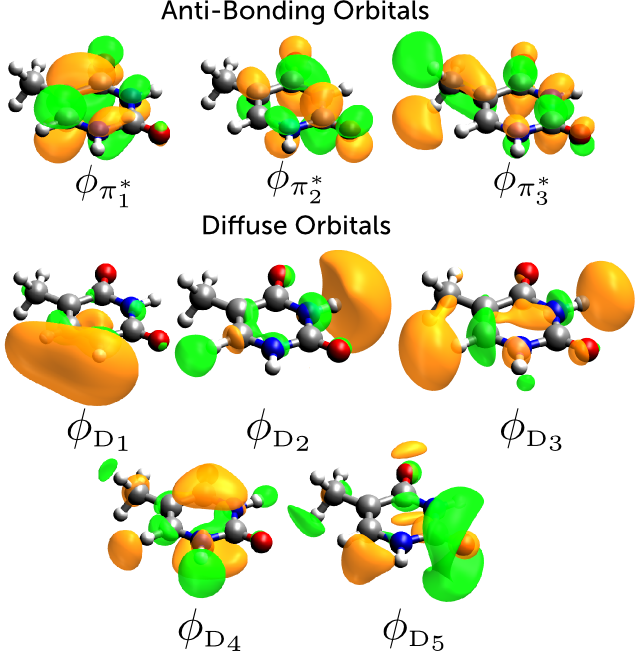
\includegraphics[width=8.8cm]{ThymineVirtuals.png}
\caption{Relevant virtual orbitals for thymine numbered in according to the orbital energy. Orbitals with obvious $\pi^*$ character are labeled as such, while orbitals where electron density is diffused  are labeled as D.}
\label{fig:thyminevirtuals}
\end{figure}
  \begin{figure}[!hb]
\centering
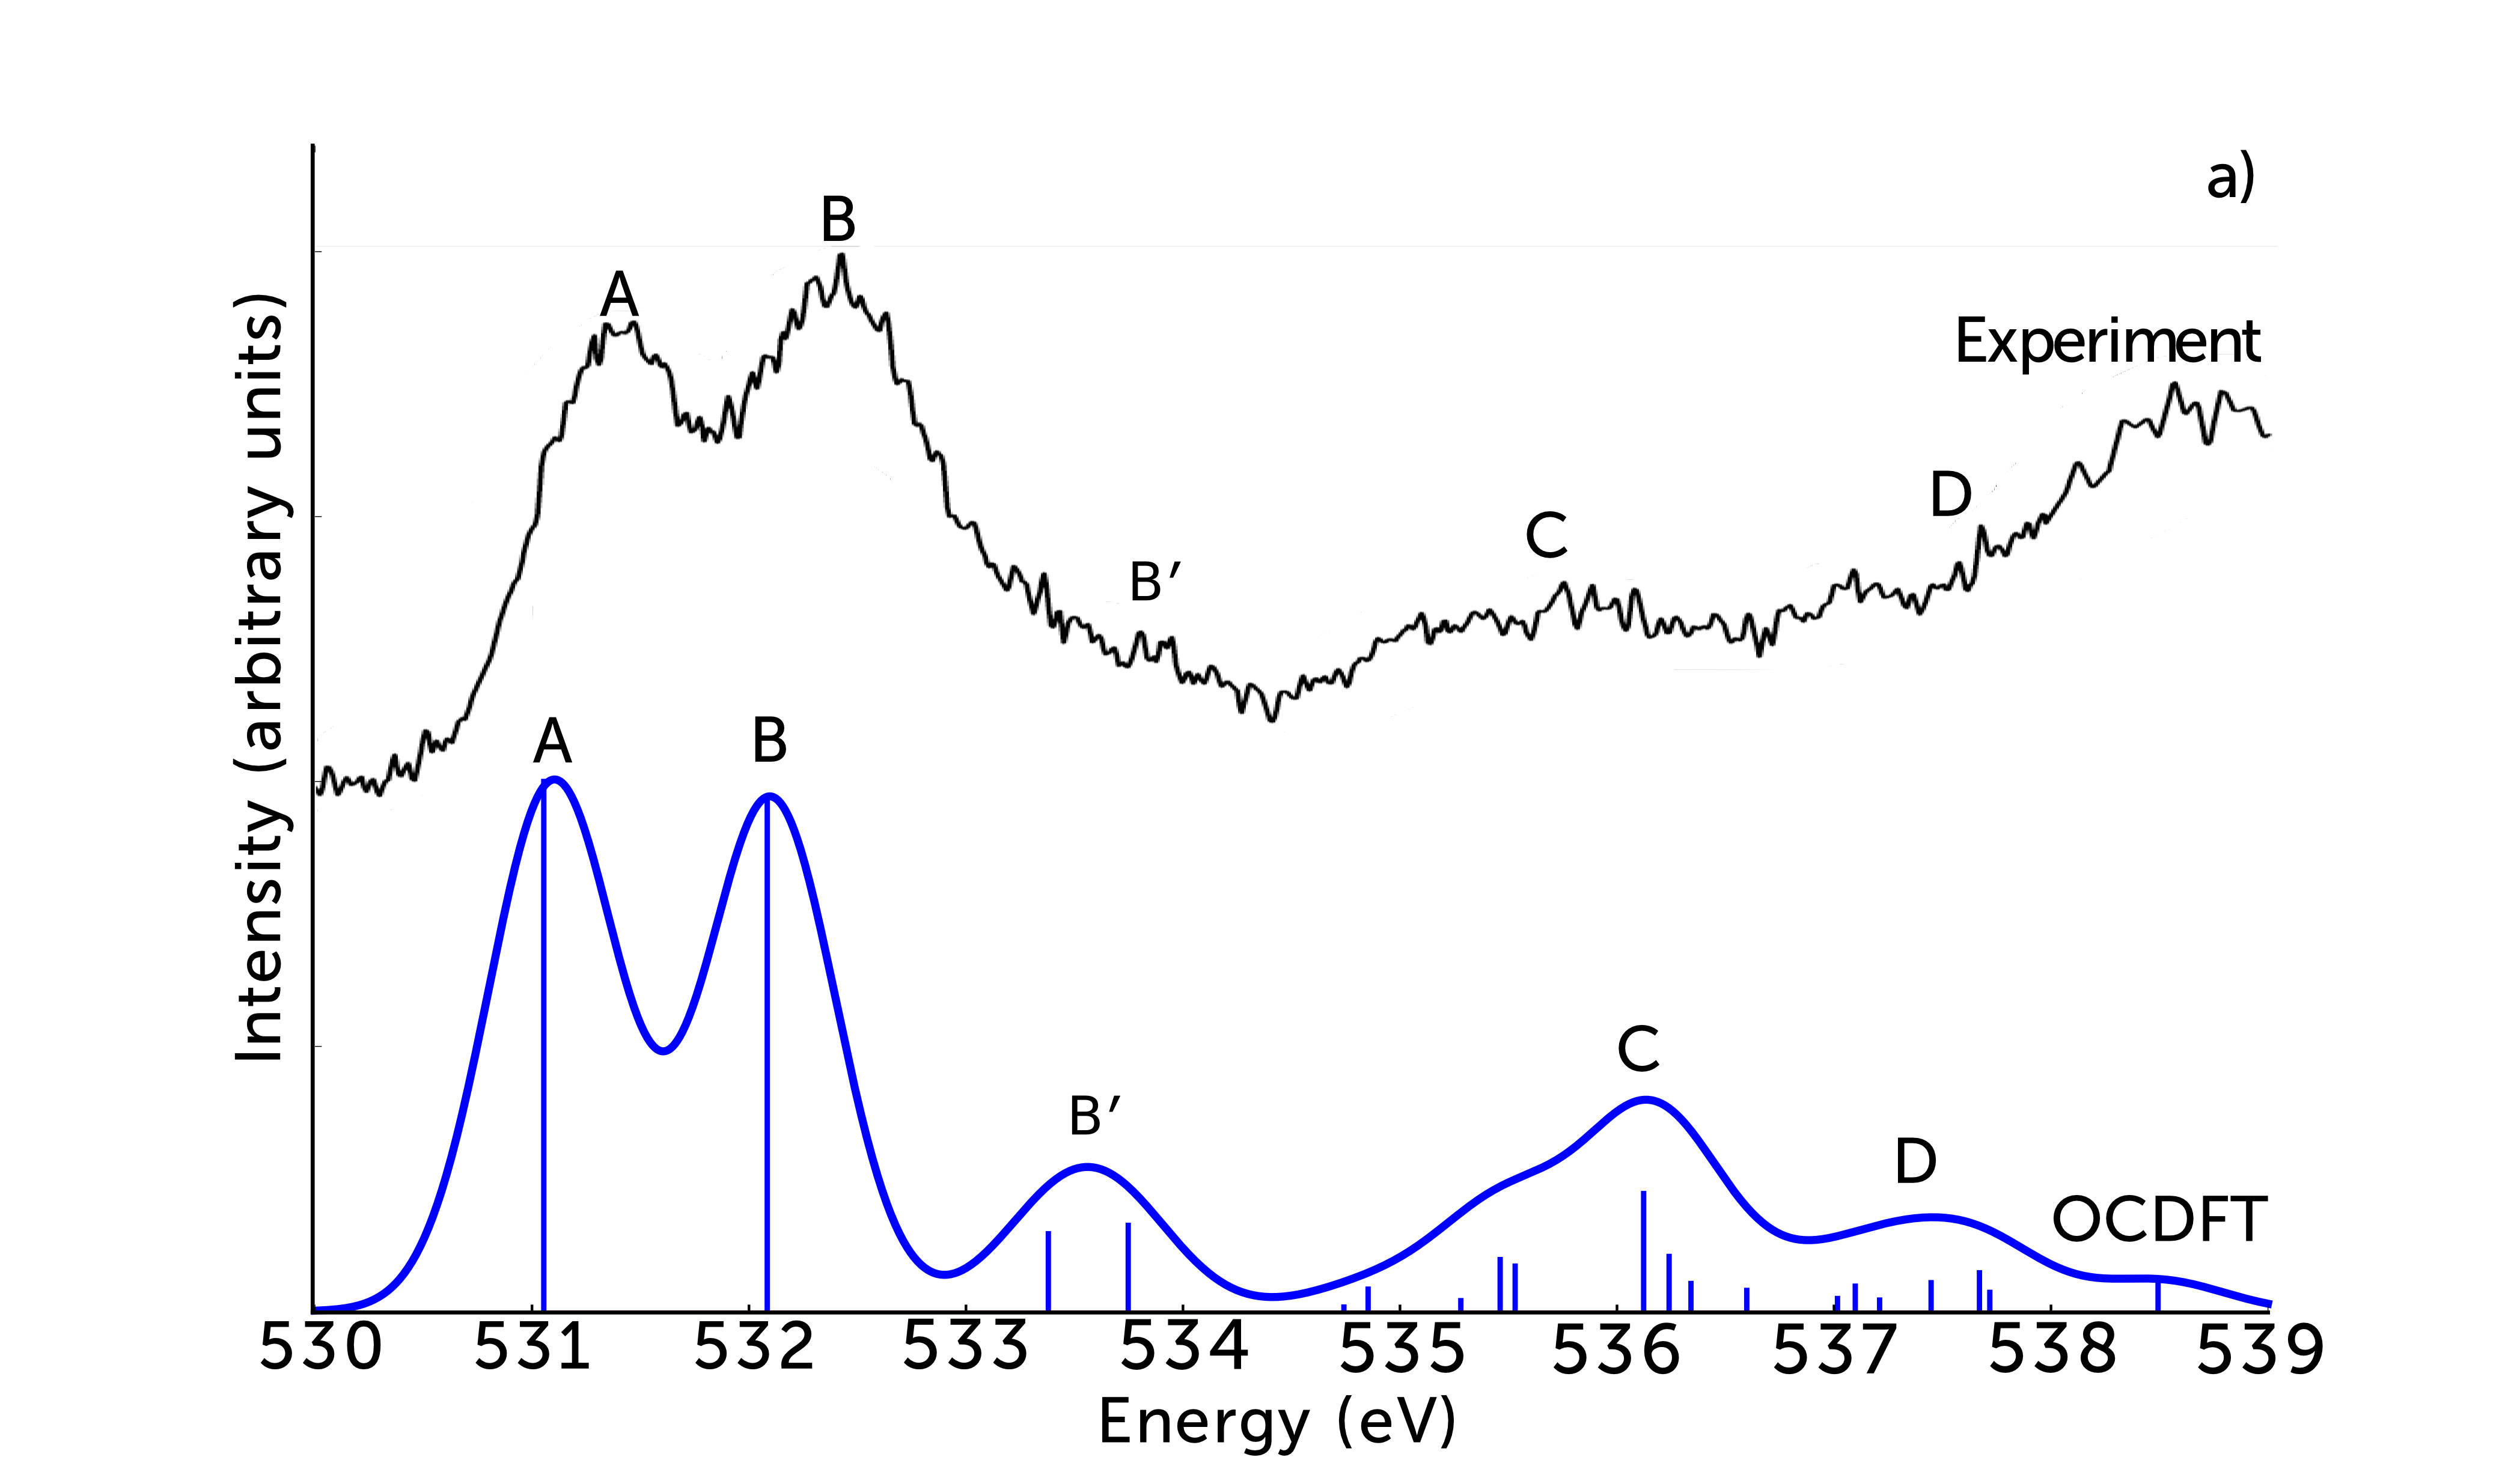
\includegraphics[width=8.8cm]{ThymineOKexperiment.png}\\
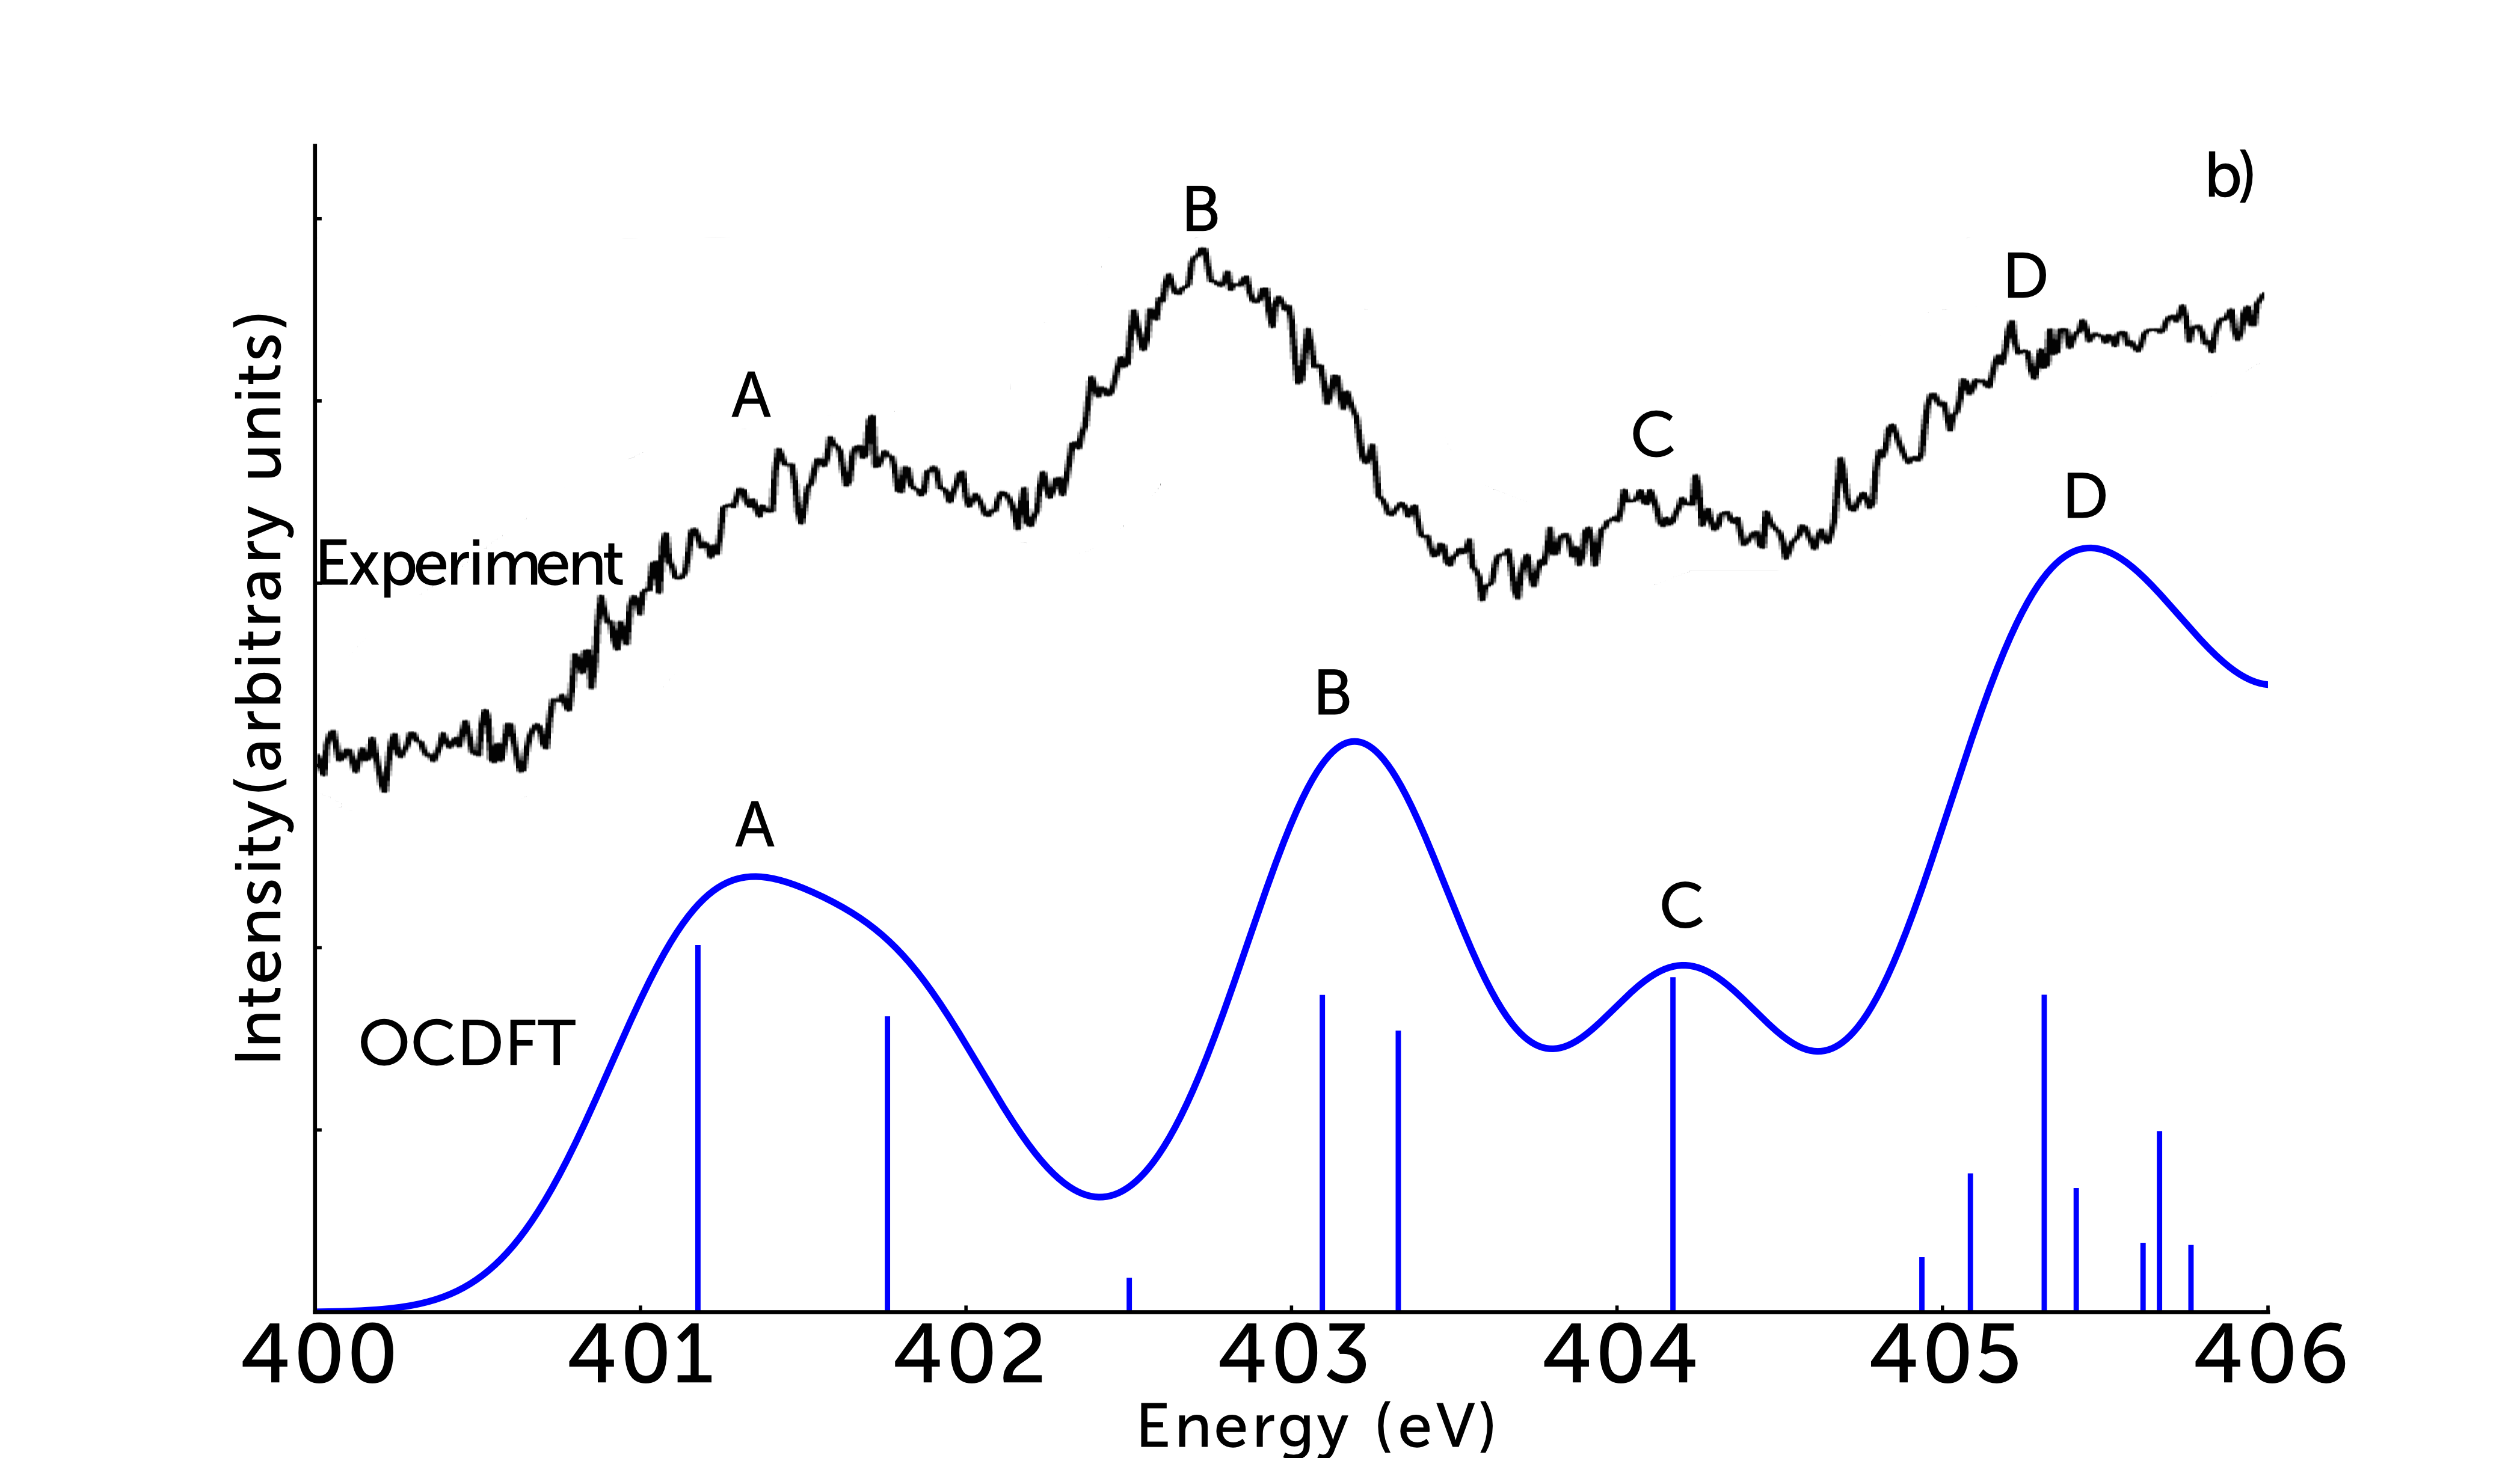
\includegraphics[width=8.8cm]{ThymineNKexperiment.png} \\
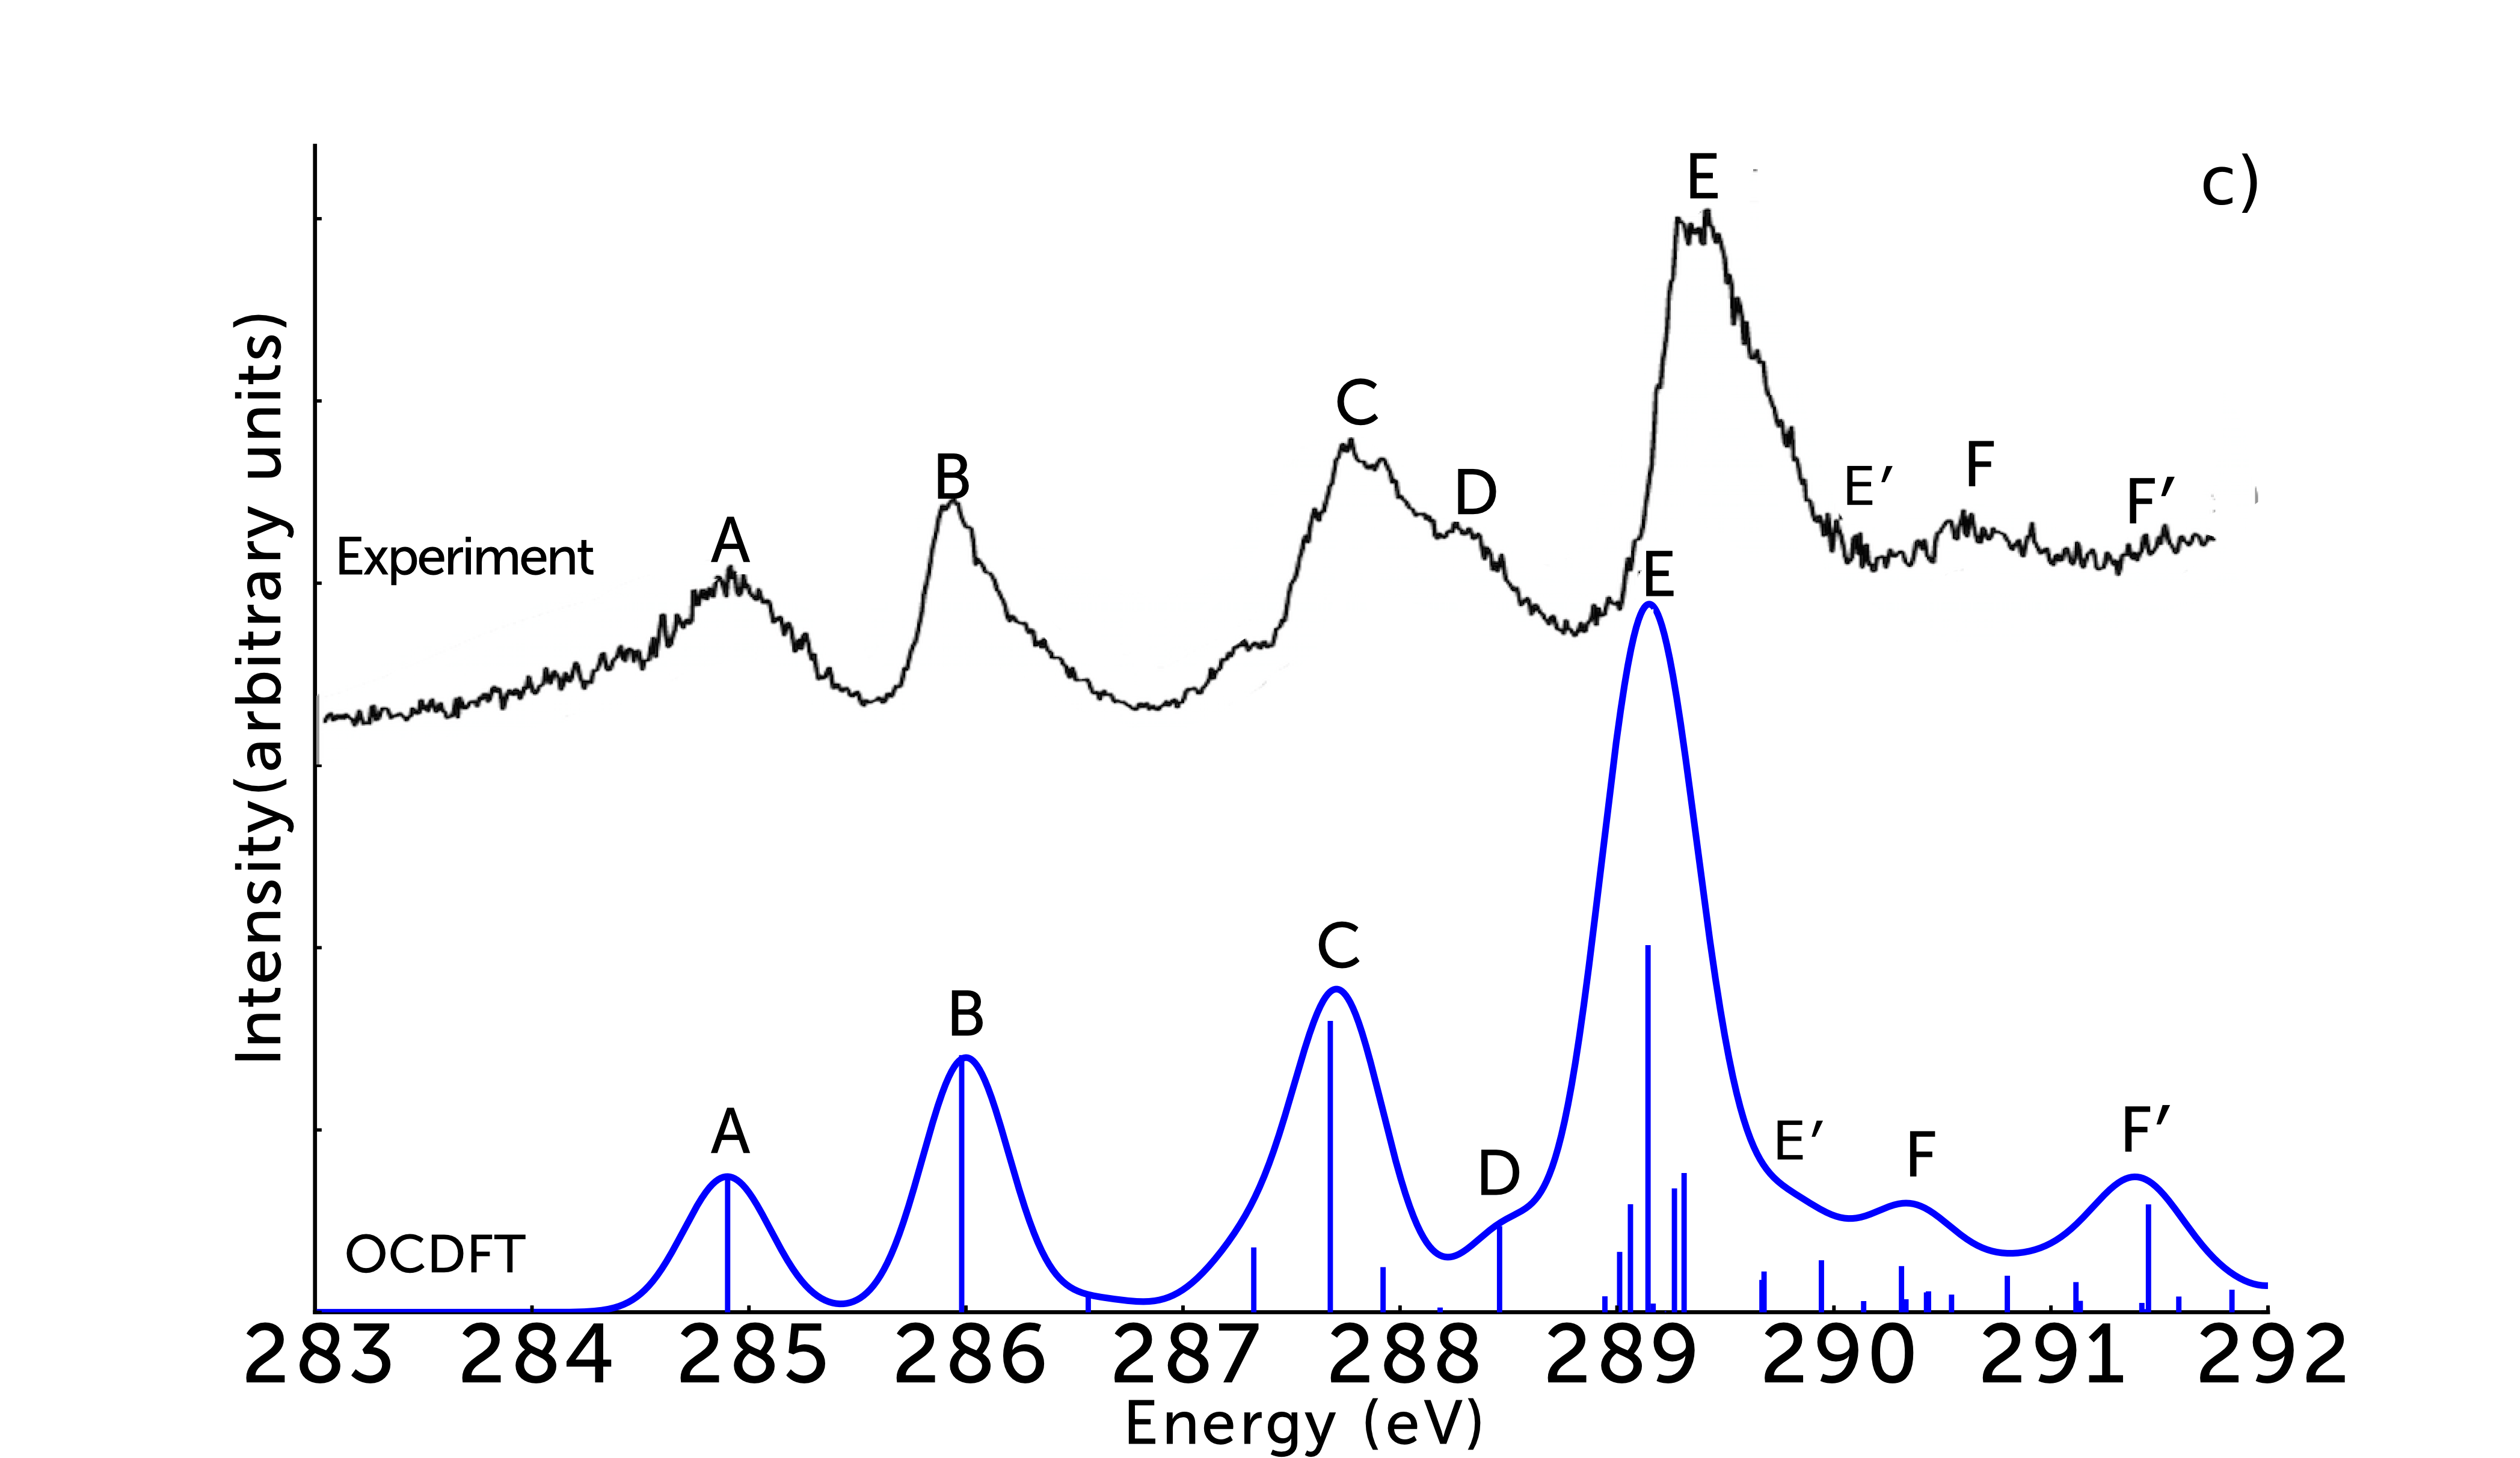
\includegraphics[width=8.8cm]{ThymineCKexperiment.png}
\caption{Core excited states for thymine computed using B3LYP functional and def2-TZVP basis set. The OCDFT oxygen and nitrogen K-edge spectra were convoluted with a Gaussian function with full width at half maximum (FWHM) equal to 0.3 eV, while the carbon spectrum uses a Gaussian with FWHM equal to 0.2 eV. The experimental spectra are reproduced with permission from Ref. \citenum{plekan_theoretical_2008}.}
\label{figure:Thymine}
\end{figure}
\subsubsection{Thymine Oxygen K-Edge}
\ Figure \ref{figure:Thymine}a displays the experimental and theoretical oxygen K-edge \bibnote{Spectra resulting from inner-shell ionizations are commonly referred to as K, L, or M edges depending on which core-shell is involved in the excitation. This nomenclature is simply derived from the Barkla labeling scheme for the X-ray series, and we will routinely employ it to refer to specific spectra.} spectra of thymine. The low energy regime of the oxygen K-edge is dominated by two high intensity peaks. Peak A results from the transition O$_2$ $\rightarrow$ $\phi_{\pi^*_2}$, while peak B results from the transition O$_1$ $\rightarrow$ $\phi_{\pi^*_1}$ with a peak intensity that is roughly equal to that of peak A. Experimentally, A and B are centered at 531.4 eV and 532.3 eV, respectively, and are predicted by OCDFT to within 0.3 eV. The  O$_2$ $\rightarrow$ $\phi_{\pi_2^*}$ transition is predicted as the peak of highest intensity with f$_{\rm abs}$ = 0.02, and this result is consistent with the ADC(2) analysis performed by Plekan et al. \cite{plekan_theoretical_2008} which predicts f$_{\rm abs}$ = 0.03. According to OCDFT, the shoulder feature B$^{\prime}$ is composed of O$_1$ $\rightarrow$ $\phi_{\pi^*_2}$ and O$_2$ $\rightarrow$ $\pi^*_1$ transitions predicted to have a fairly strong oscillator strength (f$_{\rm rel}$ $\approx$ 0.2), which is in discrepancy with the low intensity peaks observed in the experimental spectrum.  As stated earlier, excitations of weaker intensity are characteristic of the higher energy regime of the K-edge and have been attributed to strong mixing of core-valence excited states with Rydberg excited states of similar energy.\cite{robin_rydberg_1975} This strong mixing causes excitations to be spread out over several different final states, resulting in transitions of weak intensity. The mixing in this region of the spectrum makes it difficult to classify specific transitions experimentally. OCDFT results show that peak C is largely composed of a mixture of diffuse Rydberg excitations within the energy interval of 534.7 to 536.4 eV. While the majority of the contributions to peak D, are excitations to $\phi_{\rm D_2}$ and $\phi_{\rm D_5}$, with f$_{\text{rel}}$ $<$ 0.1, peaks C and D both have $\phi_{\pi^*_3}$ character. In both cases, these resonances are weak and overshadowed by multiple Rydberg transitions in both cases. 
\newcolumntype{.}{D{.}{.}{-1}}
   \begin{table}[!ht]
   \footnotesize
            \caption{Calculated (B3LYP/def2-TZVP) and experimental thymine oxygen, nitrogen, and carbon core excitation energies ($\omega_{fi}$, in eV) and relative oscillator strengths ($f_{\rm real}$).  For each calculated transition, we also report the label of the core atomic orbital ($\phi_{\rm h}$) and the  largest ground-state virtual orbital contribution to the particle orbital ($\phi_{\rm p}$).}
 \centering
     \begin{tabular*}{8.5cm}{@{\extracolsep{\fill} }cccrccc}
     \hline
     \hline\\[-8pt]
     \multicolumn{6}{c}{
% \parbox[c]{1em}{
 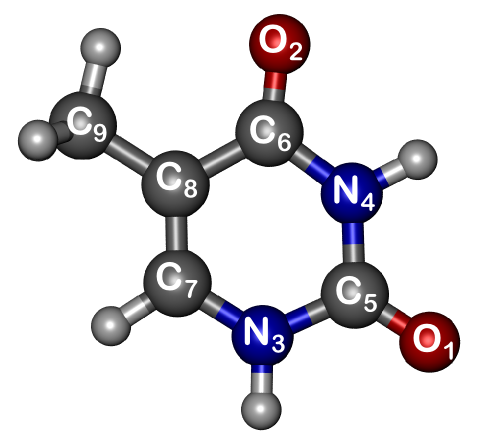
\includegraphics[width=3.cm]{ThymineNumbering.png}
 }\\
 \hline
   \multicolumn{4}{c}{OCDFT} &\multicolumn{2}{c}{Experiment} \\
 $\phi_{\rm h}$ &  $\phi_{\rm p}$ & $\omega_{fi}$ & f$_{\rm rel}$ & Peak &  $\omega_{fi}$   \\[1pt]
   \hline
    \multicolumn{6}{c}{\textbf{Oxygen K-Edge}} \\[0.05in]
    O$_2$
 &   81.8$\%$ $\pi_1^*$  & 531.1 & 1.000 & A  & 531.4 \\[0.05in]
    O$_1$
 &   64.0$\%$ $\pi_2^*$  & 532.1 & 0.995 & B & 532.3 \\[0.05in]
    O$_1$
 &   71.2$\%$ $\pi_1^*$  & 533.4 & 0.130 & \multirow{2}{*}{B$^{\prime}$} & \multirow{2}{*}{533.8}  \\ % $\approx$
    O$_2$
 &   78.3$\%$ $\pi_2^*$  & 533.8 & 0.143\\[0.05in]
    O$_1$
 &   69.5$\%$ $\rm D_3$  & 535.5 & 0.092   & \multirow{3}{*}{C} & \multirow{3}{*}{535.7}  \\
    O$_1$
 &   76.0$\%$ $\pi_3^*$  & 536.1 & 0.212 \\
    O$_2$
 &   69.0$\%$ $\pi_3^*$  & 536.2 & 0.090 \\[0.05in]
    O$_1$
 &   83.5$\%$ $\rm D_2$  & 537.1 & 0.040 & \multirow{3}{*}{D} & \multirow{3}{*}{537.1} \\
    O$_1$
 &   35.6$\%$ $\rm D_5$  & 537.5 & 0.049 \\
    O$_2$
 &   44.0$\%$ $\rm D_5$  & 537.7 & 0.065 \\[0.05in]
  \multicolumn{6}{c}{\textbf{Nitrogen K-Edge}} \\[0.05in]
     N$_4$
 &   81.8$\%$ $\pi_1^*$  & 401.2 & 0.998 & \multirow{2}{*}{A} & \multirow{2}{*}{401.7} \\
    N$_3$
 &   64.0$\%$ $\pi_2^*$  & 401.8 & 0.802 
 \\[0.05in]
    N$_4$
 &   78.3$\%$ $\pi_2^*$  & 402.5 & 0.087 & \multirow{3}{*}{B} & \multirow{3}{*}{402.7}\\
    N$_3$
 &   77.0$\%$ $\rm D_1$  & 403.1 & 0.895 \\
    N$_4$
 &   65.9$\%$ $\rm D_1$  & 403.3 & 0.790 
 \\[0.05in]
    N$_4$
 &   44.1$\%$ $\rm D_3$  & 404.2 & 0.894 & C & 404.1 
 \\[0.05in]
    N$_3$
 &   69.5$\%$ $\rm D_3$  & 405.1 & 0.370  & \multirow{3}{*}{D} & \multirow{3}{*}{405.5} \\
    N$_4$
 &   86.3$\%$ $\rm D_2$  & 405.3 & 0.852 \\
    N$_3$
 &   71.2$\%$ $\pi_1^*$  & 405.7 & 0.502 \\[0.05in]
   \multicolumn{6}{c}{\textbf{Carbon K-Edge}} \\[0.05in]
       C$_8$
 &   92.1$\%$ $\pi_1^*$  & 284.9 & 0.328 & A & 284.9  
  \\[0.05in]
    C$_7$
 &   95.9$\%$ $\pi_1^*$  & 286.0 & 0.635 & B & 285.9
  \\[0.05in]
    C$_8$
 &   97.6$\%$ $\pi_2^*$  & 287.3 & 0.140   & \multirow{3}{*}{C} & \multirow{3}{*}{287.8}  \\
    C$_6$
 &   81.8$\%$ $\pi_1^*$  & 287.7 & 0.770 \\
    C$_9$
 &   89.9$\%$ $\pi_1^*$  & 287.9 & 0.108  
  \\[0.05in]
     C$_9$ &   87.7$\%$ $\rm D_1$  & 288.5 & 0.205 & D & 288.4
   \\[0.05in]
    C$_5$
 &   64.0$\%$ $\pi_2^*$  & 289.1 & 1.000 & \multirow{3}{*}{E} & \multirow{3}{*}{289.4} \\
    C$_9$
 &   63.1$\%$ $\pi_3^*$  & 289.3 & 0.294 \\
    C$_9$
 &   49.5$\%$ $\rm D_2$  & 289.3 & 0.343 
 \\[0.05in]
    C$_8$
 &   33.3$\%$ $\rm D_4$  & 290.3 & 0.098 & \multirow{3}{*}{F} &  \multirow{3}{*}{290.7}  \\
    C$_9$
 &   30.5$\%$ $\rm D_4$  & 290.4 & 0.042 \\
    C$_7$
 &   71.6$\%$ $\rm D_3$  & 290.4 & 0.041 \\
\hline\hline% \\
%\hline
%\hline
   \end{tabular*}
   \label{table: thymine_k_oxygen}
   \end{table}
\subsubsection{Thymine Nitrogen K-Edge} \ The K-edge pictured in Figure \ref{figure:Thymine}b is characterized by four distinct spectral peaks. These lowest energy contributions to peak A are excitations from N$_3$ and N$_4$ to $\phi_{\pi^*_2}$. OCDFT predicts their excitation energies to be 401.8 eV and 401.2 eV, respectively. The experimental peak maximum is at 401.7 eV, which agrees well with the Gaussian profile shown in the OCDFT spectrum. Rydberg transitions from the N$_3$ and N$_4$ to $\phi_{\rm D_1}$ are the dominant resonances contributing to the character of peak B, along with a valence excitation N$_4$ $\rightarrow$ $\phi_{\pi^*_1}$ predicted at 402.5 eV. This agrees well with the experimental peak assignment at 402.7 eV. A very intense N$_4$ $\rightarrow$ $\phi_{\rm D_3}$ transition accounts for the peak at 404.1 eV. OCDFT simulates this peak perfectly with a Gaussian centered at 404.2 eV. peak D is the amalgamation of two $\pi^*$ resonances and multiple Rydberg states with the $\pi^*$ resonances being the transitions of strongest intensity. Excitation energies of these $\pi^*$ resonances agree well with the experimental peak assignment at 405.5 eV, with N$_4$ $\rightarrow$ $\phi_{\pi^*_3}$ at 405.3 eV and N$_3$ $\rightarrow$ $\phi_{\pi^*_1}$ at 405.7 eV.
\subsubsection{Thymine Carbon K-Edge} \
   The shape of the carbon K-edge displayed in Figure \ref{figure:Thymine}c is governed by four strong $\pi^*$ resonances. Unique to the carbon K-edge is the fact that the strongest transition is not the lowest energy $\pi^*$ resonance, the C$_5$ $\rightarrow$ $\phi_{\pi_1^*}$ transition is a relatively high energy excitation and produces the strongest peak intensity, despite close proximity to several Rydberg states. Peak A at 284.9 eV is the result of the transition C$_8$ $\rightarrow$ $\phi_{\pi_2^*}$, the position of this peak is predicted exactly by OCDFT. A slightly stronger transition at 285.9 eV is mostly due to a  C$_7$ $\rightarrow$ $\phi_{\pi_2^*}$ excitation, with small contribution from another $\phi_{\pi_2^*}$ transition resulting from an excitation from the C$_9$ core. Peaks C and D have experimental peak maxima at 287.8 eV and 288.4 eV respectively, and blend together to form one band. Both contributions to the spectral band are represented well by OCDFT.
%The most prominent contributor to Peak C is the excitation from C$_6$ $\rightarrow$ $\pi^*_3$, while Peak D is the result of a C$_9$ $\rightarrow$ $\pi^*_3$. 
Peak E is mostly composed of core excitations to diffuse orbitals, however these transitions have relatively weak intensities compared to the strong $\phi_{\pi_2^*}$ transition predicted at 289.1 eV. Excitations to diffuse orbitals are dominant contributors to the remaining spectral features F and F$^{\prime}$.
%Peak E is mostly a fusion of core excitations to diffuse orbitals, however these transitions have relatively weak intensities compared to the dominant $\pi_1^*$ character present in the region. There is also $\pi^*_2$ character here, however the oscillator strength of this transition is very small compared to the Rydberg contributions. A small shoulder E$^{\prime}$ is present at the base of peak E, and is mostly due to a weak transition from C$_6$ $\rightarrow$ $\pi_1^*$.  Rydberg states dominate the rest of the spectra, and are provide the strongest contributions to Peak F and the shoulder feature at F$^{\prime}$. 
\begin{figure}[!t]
\centering
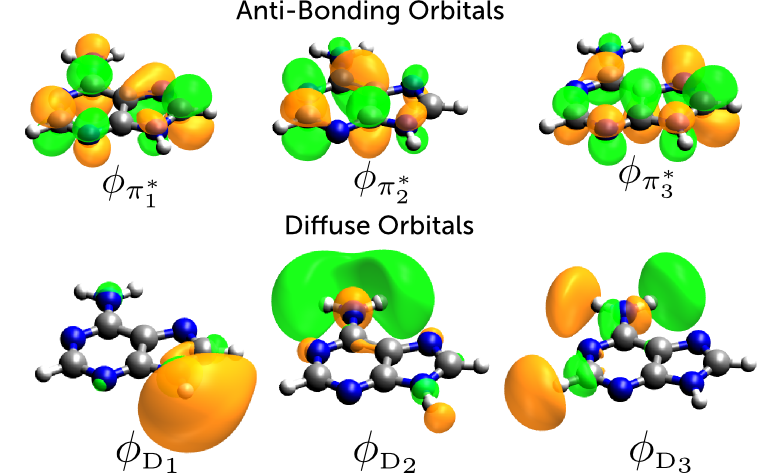
\includegraphics[width=8.8cm]{AdenineVirtuals.png} \\
\caption{Relevant virtual orbitals for adenine numbered according to the orbital energy. Orbitals with obvious $\pi^*$ character are labeled as such, while orbitals where electron density is mostly diffused on the outside of the molecule are labeled as $\phi_D$.}
\label{figure:adeninevirtuals} 
\end{figure}
\subsubsection{Adenine Nitrogen K-Edge}
   \ Figure \ref{figure:Adenine}a displays the nitrogen k-edge of adenine computed with OCDFT. The most dominant feature of the spectrum, peak A, is experimentally classified at 399.5 eV, OCDFT predicts that this feature is a result of core-valence excitations originating from three of the four nitrogens on the purine ring system (N$_4$, N$_3$, N$_5$). The largest contributor being a transition from N$_5$ $\rightarrow$ $\phi_{\pi_2^*}$ predicted at 399.4 eV, which agrees well with the experimental classification for the peak. An apparent shoulder feature with fairly weak oscillator strength is present in the experimental spectrum in the region from 399.8 -- 400.4 eV. OCDFT represents this feature well, with two weak $\pi^*$ resonances resulting from the two nitrogens on the six-membered ring. A few rising shoulder features are shown in the experimental spectrum in the region from 401.0 eV -- 401.3 eV, OCDFT predicts a N$_3$ $\rightarrow$ $\phi_{\pi_2^*}$ transition in this region with a relative oscillator strength of 0.094. Peak B is a mixture of transitions to $\pi^*$ orbitals as well as diffuse orbitals, with the $\pi^*$ resonances being the prominent contributors. 
%The prominent contributors are $\pi^*$ resonances with the N$_1$ $\rightarrow$ $\pi^*$ being the most intense at 401.8 eV. This is commensurate to the experimental peak assignment at 401.9, the peak height relative to peak A is also in good agreement with experiment. 
The experimental spectrum shows a relatively weak resonance around 403.0 (peak C).  We predict that the dominant contributor to peak C is a transition from N$_2$ $\rightarrow$ $\phi_{\rm D_3}$, the intensity of which, that rivals the strongest transition (peak A f$_{\rm rel}$ = 0.925). This peak intensity is contrary to the experimental spectrum which shows peak C  as a superposition of weak transitions. The highest energy transitions are all weak transitions to mostly orbitals of diffuse character, with transitions getting more intense as they approach 405.0 eV. 
 \begin{figure}[!t]
\centering
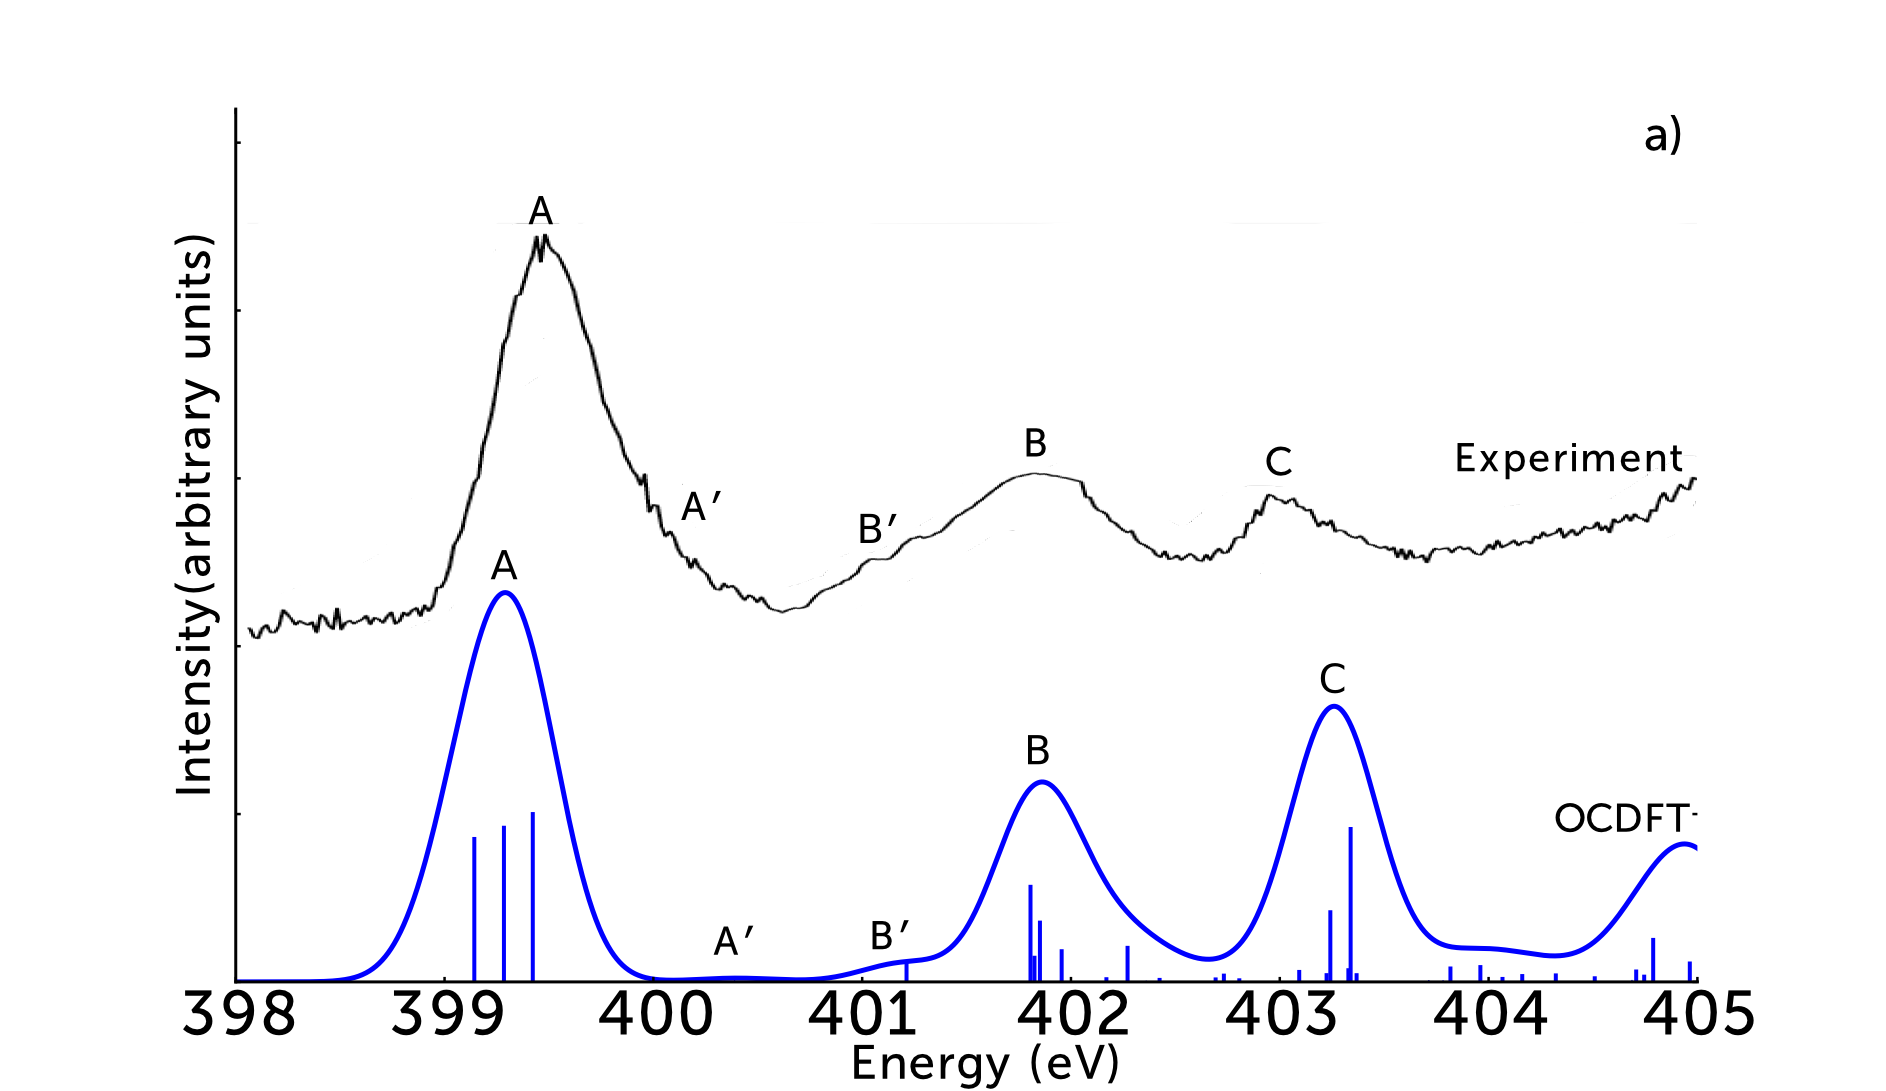
\includegraphics[width=8.8cm]{AdenineNKexperiment.png} \\
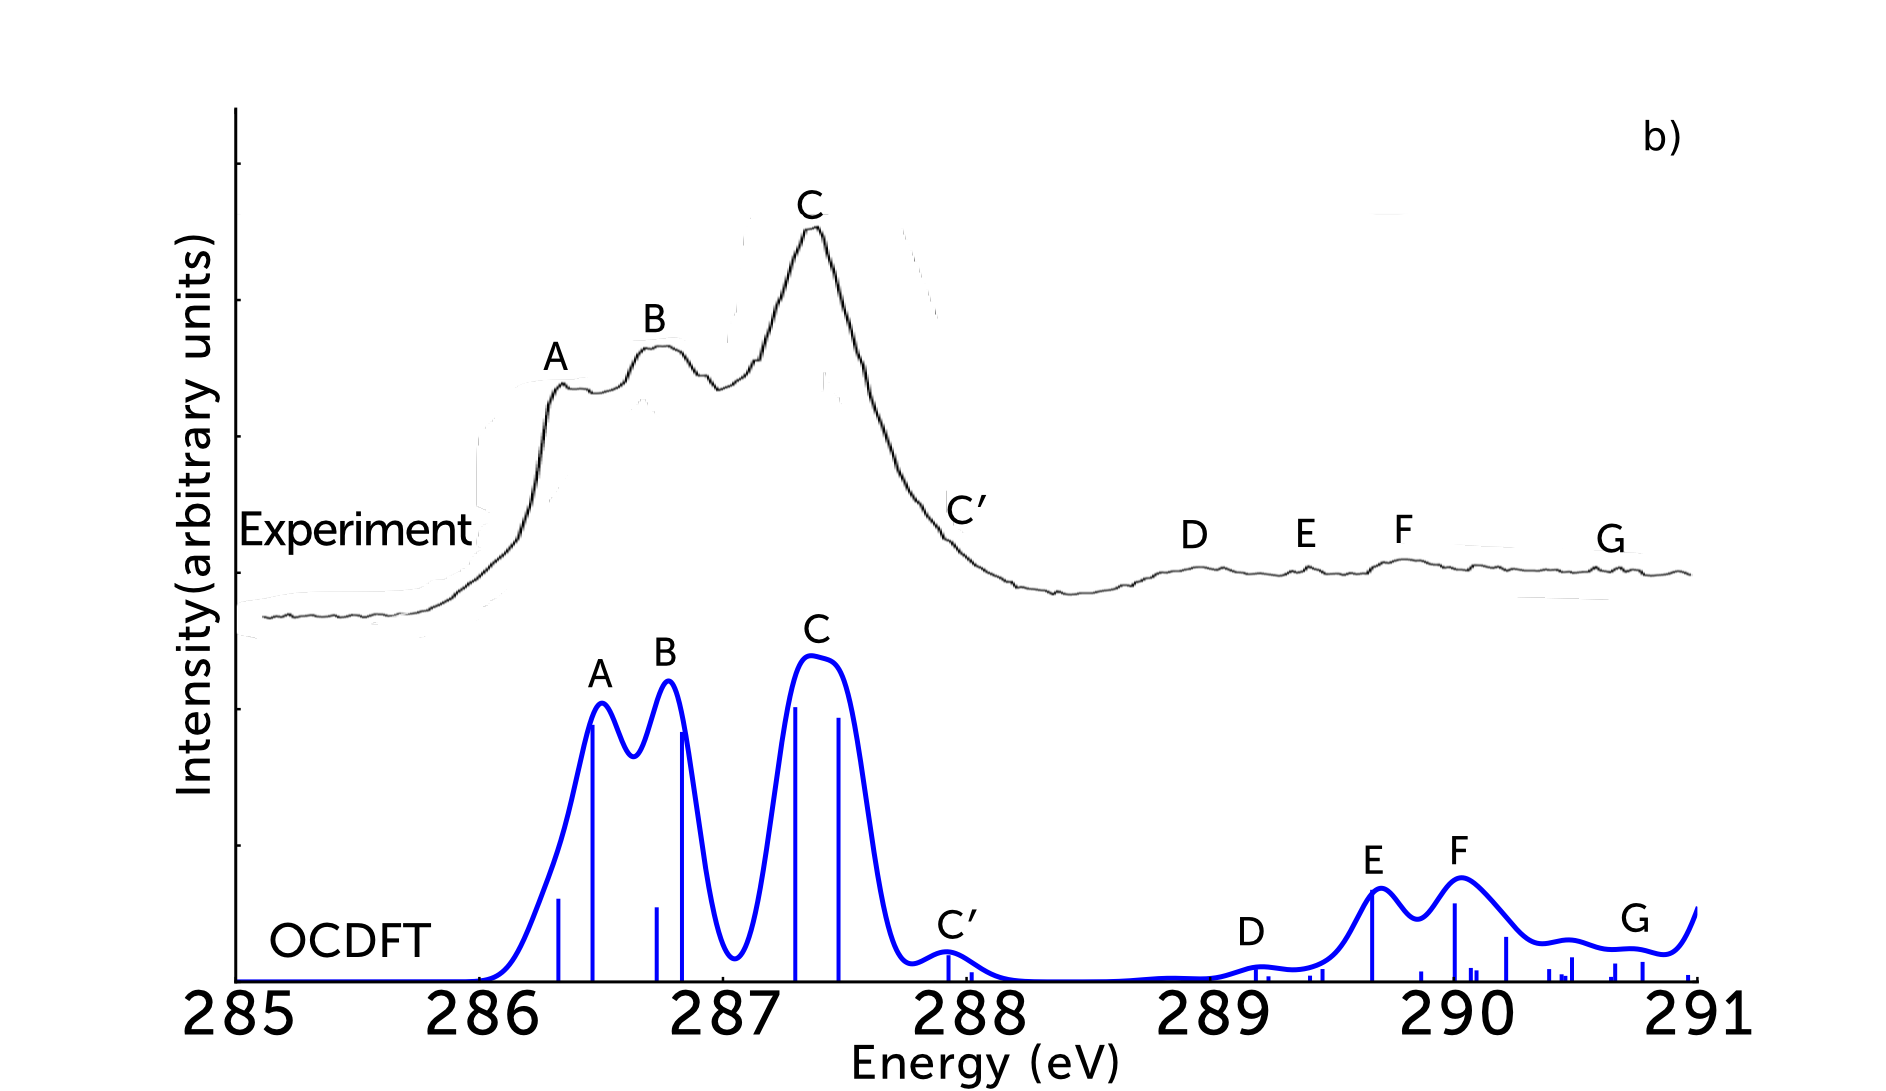
\includegraphics[width=8.8cm]{AdenineCKexperiment.png}
\caption{Core excited states for adenine computed using B3LYP functional and def2-TZVP basis set. 
The OCDFT carbon and nitrogen K-edge spectra were convoluted with a Gaussian function with full width at half maximum (FWHM) equal to 0.3 eV.  The experimental spectra are reproduced with permission from Ref. \citenum{plekan_theoretical_2008}.}
\label{figure:Adenine}
\end{figure} 
%The experimental spectra shows that these transitions get more intense as they appraoch 405.0 eV, which is represented well in our calculations. \\
\subsubsection{Adenine Carbon K-Edge}
\ Fig. \ref{figure:Adenine}b compares the OCDFT and experimental carbon K-edge of adenine. The experimental carbon K-edge for adenine is dominated by a large single band with three distinct resonances in the low energy regime. The theoretical spectrum shows peaks A and B, blending together into a single band, the experimental spectrum shows these peaks at similar intensities, with peak B being slightly more intense, this is represented well in our calculated spectrum. Spectral positions for peaks A, B, and C are all in good agreement with experiment, 
\begin{table}
\caption{Comparison of the most intense transitions at each edge of the thymine and adenine spectra. OCDFT assignments and energies (in eV) are shown and are compared to the most intense transitions from the theoretical ADC(2) spectra reported in Ref~\citenum{plekan_theoretical_2008}.}
\small
\centering
\begin{tabular}{ccc}
\hline
\hline
K-Edge & OCDFT & ADC(2) \\
\hline
\multicolumn{3}{c}{\bf Thymine} \\
Oxygen  & O$_2$ $\rightarrow$ $\pi^*_1$ (531.1) &  O$_2$ $\rightarrow$ $\pi^*_1$ (531.4)  \\
Nitrogen  & N$_4$ $\rightarrow$ $\pi^*_1$ (401.2) & N$_4$ $\rightarrow$ $\pi^*_1$ (401.5) \\
Carbon  & C$_5$ $\rightarrow$ $\pi^*_2$ (289.1) & C$_5$ $\rightarrow$ $\pi^*_2$ (289.7) 
\\[2pt]
\multicolumn{3}{c}{\bf Adenine} \\
Nitrogen &  N$_5$ $\rightarrow$ $\pi^*_2$ (399.4) & N$_5$ $\rightarrow$ $\pi^*_2$ (399.6) \\
Carbon  & C$_6$ $\rightarrow$ $\pi^*_1$ (287.3) & C$_6$ $\rightarrow$ $\pi^*_1$ (287.4)\\[2pt]
\hline
\hline
\end{tabular}
\label{table: assignment_comparison}
\end{table}
%Peak A has a maximum located at 286.4 eV in the experimental spectra, our calculations agree well with this predicting a transition from C$_9$ $\rightarrow$ $\pi_1^*$ at 286.5 eV as the dominant contributor. Similar agreement is seen with peak B located at 286.8 eV, with OCDFT predicting its dominant contributor to be a transition from C$_7$ $\rightarrow$ $\pi_1^*$.  The OCDFT spectra predicts peak C as the most intense spectral feature, which is consistent with experiment. 
however, the oscillator strength is inconsistent with experimental peak intensities. According to the experimental results, peak C should be roughly 50\% more intense than the adjacent peak B. OCDFT predicts that the C$_6$ $\rightarrow$ $\phi_{\pi^*_1}$ that dominates peak C is only slightly more intense than the dominant contributions to peaks A and B. A very weak shoulder feature is present on the falling edge of peak C, we denote this feature as C$^{\prime}$ and it is represented well by OCDFT. This shoulder results from $\pi^*$ transitions with hole orbitals located on the bridge carbons (C$_8$ and C$_{10}$) and a carbon located on the six-member ring (C$_9$). Peaks D-G were not assigned due to their low intensities. OCDFT reveals that peak D is a very weak spectral feature with dominant contributions from excitations to diffuse orbital $\phi_{\rm D_3}$. Peaks E and F are also weak spectral features resulting mostly from transitions to diffuse orbitals. Every transition with energy higher than peak F is extremely weak 
 \begin{table}[!ht]
 \footnotesize
\caption{Calculated (B3LYP/def2-TZVP) and experimental adenine nitrogen and carbon core excitation energies ($\omega_{fi}$, in eV) and relative oscillator strengths ($f_{\rm real}$).  For each calculated transition, we also report the label of the core atomic orbital ($\phi_{\rm h}$) and the  largest ground-state virtual orbital contribution to the particle orbital ($\phi_{\rm p}$).
}
 \centering
     \begin{tabular*}{8.5cm}{@{\extracolsep{\fill} }cccccc}
     \hline\hline\\[-8pt]
     \multicolumn{6}{c}{
 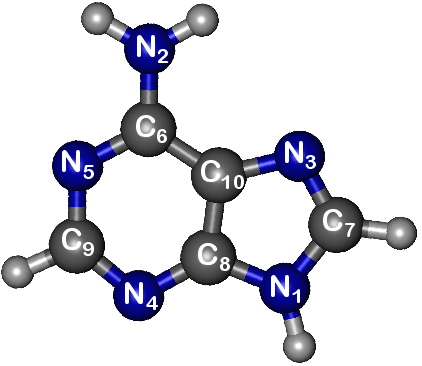
\includegraphics[width=3.5cm]{AdenineNumbering.png}}\\
     \hline
   \multicolumn{4}{c}{OCDFT} &\multicolumn{2}{c}{Experiment} \\
 $\phi_{\rm h}$ &  $\phi_{\rm p}$ & $\omega_{fi}$ & f$_{\rm rel}$ & Peak &  $\omega_{fi}$   \\[1pt]
   \hline
    \multicolumn{6}{c}{\textbf{Nitrogen K-Edge}} \\[0.05in]
    N$_4$
 &   81.0$\%$ $\pi_1^*$  & 399.1 & 0.825 & \multirow{3}{*}{A} & \multirow{3}{*}{399.5} \\
    N$_3$
 &   63.7$\%$ $\pi_1^*$  & 399.3 & 0.915 \\
    N$_5$
 &   92.6$\%$ $\pi_2^*$  & 399.4 & 1.000 
\\[0.05in]
    N$_5$
 &   92.4$\%$ $\pi_1^*$  & 399.7 & 0.001 & \multirow{2}{*}{A$^{\prime}$} & \multirow{2}{*}{400.4}  \\ %$\approx$ 
    N$_4$
 &   98.9$\%$ $\pi_2^*$
 & 400.4 & 0.019 
 \\[0.05in]
    N$_3$
 &   81.6$\%$ $\pi_2^*$  & 401.2 & 0.094 & B$^{\prime}$ & 401.3 
 \\[0.05in]
    N$_2$
 &   82.1$\%$ $\pi_1^*$  & 401.4 & 0.351 & \multirow{3}{*}{B} & \multirow{3}{*}{401.9}\\
    N$_1$
 &   69.3$\%$ $\pi_1^*$  & 401.8 & 0.587 \\
    N$_2$
 &   78.4$\%$ $\rm D_2$  & 402.3 & 0.204
 \\[0.05in] 
    N$_1$
 &   74.8$\%$ $\pi_2^*$  & 403.1 & 0.109 & \multirow{3}{*}{C} & \multirow{3}{*}{403.0} \\
    N$_1$
 &   87.2$\%$ $\rm D_1$  & 403.3 & 0.418 \\
    N$_2$
 &   57.1$\%$ $\rm D_3$  & 403.3 & 0.925
 \\[0.05in]
 \multicolumn{6}{c}{\textbf{Carbon K-Edge}} \\[0.05in]
     C$_{10}$
 &   92.6$\%$ $\pi_2^*$  & 286.3 & 0.270 & \multirow{2}{*}{A} & \multirow{2}{*}{286.4}\\
    C$_9$
 &   81.0$\%$ $\pi_1^*$  & 286.5 & 0.924 
 \\[0.05in]
    C$_{10}$
 &   92.4$\%$ $\pi_1^*$  & 286.7 & 0.242 &  \multirow{2}{*}{B} &  \multirow{2}{*}{286.8} \\
    C$_7$
 &   82.1$\%$ $\pi_1^*$  & 286.9 & 0.878
 \\[0.05in]
    C$_6$
 &   69.3$\%$ $\pi_1^*$  & 287.3 & 1.000 &  \multirow{2}{*}{C} &  \multirow{2}{*}{287.4}\\
    C$_8$
 &   63.7$\%$ $\pi_1^*$  & 287.4 & 0.965 
 \\[0.05in]
    C$_{10}$
 &   34.7$\%$ $\pi_3^*$  & 287.9 & 0.083 & \multirow{2}{*}{C$^{\prime}$} &  \multirow{2}{*}{288.0}\\
    C$_9$
 &   98.9$\%$ $\pi_2^*$
 & 288.0 & 0.021 
 \\[0.05in]
    C$_6$
 &   74.8$\%$ $\pi_2^*$  & 288.8 & 0.006 & \multirow{3}{*}{D} & \multirow{3}{*}{289.0} \\
    C$_{10}$
 &   36.4$\%$ $\rm D_2$  & 289.2 & 0.033 \\
    C$_8$
 &   66.2$\%$ $\pi_3^*$  & 289.2 & 0.012 
 \\[0.05in]
    C$_9$
 &   77.4$\%$ $\pi_3^*$  & 289.4 & 0.010 & \multirow{3}{*}{E} \\
    C$_7$
 &   87.1$\%$ $\pi_2^*$  & 289.4 & 0.029 \\
    C$_7$
 &   57.1$\%$ $\rm D_3$  & 289.7 & 0.291 
 \\[0.05in] 
    C$_9$
 &   80.2$\%$ $\rm D_1$  & 290.0 & 0.225 & \multirow{3}{*}{F} \\
    C$_8$
 &   90.2$\%$ $\rm D_1$  & 290.1 & 0.038 \\
    C$_9$
 &   83.4$\%$ $\rm D_2$  & 290.1 & 0.140
 \\[0.05in]
    C$_7$
 &   94.8$\%$ $\pi_3^*$  & 290.4 & 0.073  & \multirow{3}{*}{G} \\
    C$_6$
 &   77.2$\%$ $\pi_3^*$  & 290.7 & 0.052 \\
    C$_7$
 &   56.6$\%$ $\rm D_1$  & 290.8& 0.047 \\
 \hline
 \hline
   \end{tabular*}
 \label{fig: adenine_k_nitrogen}
 \end{table}
\subsubsection{Comparison with ADC(2) Calculations} \
Previous theoretical studies performed using ADC(2) allow us to assess the accuracy of our adenine and thymine OCDFT spectra. Three key differences in the spectra are noted here. 
The shoulder feature B$^{\prime}$ in the thymine oxygen K-Edge shown in Fig. \ref{figure:Thymine} is absent from the ADC(2) spectrum.\cite{plekan_theoretical_2008} However, a more recent study by Wenzel, Wormit, and Dreuw \cite{wenzel_calculating_2014} uses a core-valence separation (CVS) approximation to the ADC(2) working equations [CVS-ADC(2)] and predicts three excitations in this shoulder region B$^{\prime}$, all with f$_{\rm abs}$ $<$ 0.001. These weaker oscillator strengths predicted by CVS-ADC(2) are more consistent with the experimental peak profile.

The overall shape of the OCDFT thymine nitrogen K-Edge is more consistent with the experimental excitation manifold than the ADC(2) spectrum. The two peaks A and B in Fig. \ref{figure:Thymine}b have clear, distinct maxima which are produced well quantitatively with ADC(2) (after applying a uniform shift of -2.59 eV to the spectrum), strong $\pi^*$ resonances are reported near both experimental peak maxima. However, the contour of the peak is inconsistent with the experimental manifold. The ADC(2) spectrum blends into one large spectral band over the interval from 401.0 eV to 404.5 eV encompassing very closely spaced transitions, all with relatively high oscillator strengths. The extremely tight spacings and high intensities of these transitions seem to be present even in the updated CVS-ADC(2) results. The OCDFT spectrum doest not suffer from this single band issue, as the $\pi^*$ resonances in peak A are well separated from the strong $\phi_{D_1}$ transitions in peak B by more than 1.0 eV. The agreement of these results with experiment, suggest that well-separated $\pi^*$ and Rydberg resonances are more congruous with reality. However, a more detailed study of the nitrogen core excitation manifold of thymine is required to verify this observation.
ADC(2) was unable to fully resolve peaks B$^{\prime}$, B, and C in the adenine nitrogen edge shown in Fig. \ref{figure:Adenine}a. On the contrary, the OCDFT spectrum represents these peaks well, as separated spectral features, in compliance with the experimental result. 

Table \ref{table: assignment_comparison} shows a direct comparison of the OCDFT peak assignment with those obtained from ADC(2).
The comparison is restricted to the transitions of highest intensity at each K-edge. All peak assignment are consistent between the two methods and we observe only small deviations in the computed excitation energy (max error 0.54 eV).
The excellent agreement of OCDFT and ADC(2) for the highest intensity transitions is encouraging, and suggests that OCDFT could be a very useful tool to aid the assignment of NEXAS spectra.

\section{Conclusions}
\begin{comment}
Simulating NEXAS spectra is a challenge for TDDFT in tandem with conventional density functionals. Many of the efforts to overcome this problem have centered around the development of new functionals that compensate for the shortcomings of the standard GGA functionals by varying the amount of Hartree--Fock exchange and other semi-empirical parameters.
Orthogonality constrained density functional theory represents a new frontier in simulating NEXAS spectra using density functional methods.
\end{comment}

In this work we have extended OCDFT in order to calculate multiple core-excited states of first- and second-row elements.
We present two developments in OCDFT theory: 1) we show that core excitations can be easily targeted by selecting \textit{hole} orbitals that correspond to core electrons, and 2) we proposed a generalized set of orthogonality conditions that can be used to compute multiple excited states.
Our benchmark computations on core excitations from 1s and 2p orbitals of first- and second-row elements using conventional pure and hybrid functionals yield excitation energies with a mean absolute error (MAE) of 1.0 eV.
OCDFT excitation energies are slightly more accurate for first-row elements (MAE = 0.4 eV) than second-row elements (MAE = 1.6 eV).

There are a few potential sources of the remaining error in the OCDFT excitation energies.  First, is the fact that the (in principle) exact OCDFT excited state functional is approximated with the ground-state exchange-correlation functional.
Second, in our comparison with experiment we use vertical excitation energies, which neglect vibrational effects.
Third, our treatment of relativistic effects is rather simplistic.   It can only approximately account for the relaxation of the core-hole and neglects relaxation effects of valence orbitals.  Last, OCDFT cannot properly handle states that have a multideterminantal character.
We expect that the use of an approximate excited state functional is the most important source of error, and that the relativistic and configuration mixing errors are perhaps the least relevant in the case of first- and second-row elements.

The results of our formal analysis and benchmark computations suggests that there are two factors contributing to the success of OCDFT.
As in the case of other variational and constrained DFT approaches, OCDFT can properly describe charge-transfer excitations.
In addition, because the wave function of the auxiliary system is only subject to orthogonality constraints, OCDFT can fully describe orbital relaxation.
To demonstrate this, we consider the NEXAS spectrum of CO$_2$, which was suggested as a test case by one of the reviewers. 
Previous computational studies of CO$_2$\cite{Maganas:ji} showed that B3LYP/TDDFT underestimates the oxygen K-edge by 14 eV.
MRCI/CIS and MRCI/CISD underestimate the same feature by 8 and 4.2 eV, respectively.
In the case of MRCI/CIS and MRCI/CISD, the residual error was attributed to the lack of orbital relaxation effects.
A broken-symmetry OCDFT computation predicts the dominant feature of the oxygen K-edge to be at 534.4 eV, which corresponds to a deviation from experiment of 0.6 eV.  This result suggests that relaxation effects do indeed play an important role in the oxygen K-edge of CO$_2$ and that OCDFT can fully account for them.
%We interpret the excellent agreement of the OCDFT spectrum of CO$_2$ to the 

Excitation energies computed with TDDFT are significantly less accurate and degrade as one goes from first-row (MAE = 11.6 eV) to second-row elements (MAE = 31.6 eV).
Moreover, we show that in OCDFT the choice of the functional and the amount of Hartree--Fock exchange has little effect on the accuracy of the computed core excitation energies.
We perform a formal comparison of OCDFT, TDDFT, and CIS excitation energies for an excitation in which the core and virtual orbitals have zero overlap.
This analysis suggests that OCDFT's superior performance can be ascribed to the local nature of the integrals that appear in the expression for the excitation energy.

Our gas-phase OCDFT X-ray absorption spectra of thymine and adenine are in excellent agreement with experiments. 
OCDFT reproduces all the characteristic features of the NEXAS spectra of these molecules,\cite{plekan_theoretical_2008,wenzel_calculating_2014} including the distinct $\pi^*$ transitions in the lower energy regime and the significant mixing between the $\pi^*$ and diffuse orbitals in the higher energy regime of the spectra.
In addition, OCDFT assignments of the spectral features are in excellent agreement with those made using the ADC(2) method.\cite{plekan_theoretical_2008}
This study shows that our OCDFT approach for core-excited states is a practical and useful tool for the interpretation of NEXAS experiments. 
From the computational point of view, the scaling of OCDFT vs. the number of electrons ($N$) is identical to that of ground state DFT ($N^3$ and $N^4$ for pure and hybrid functionals) and it is lower than the second-order approximate coupled cluster method (CC2)\cite{christiansen_cc2_1995} and [ADC(2)], which scale as $N^5$.

Two classes of systems that are worth further exploration are transition metal complexes and open-shell molecules. Core excitations in transition metal complexes present a number of additional challenges that will require further extension of the present theory.
One of the biggest improvements that will be necessary is a proper treatment of relativistic effects.
While the scheme used in this work was sufficient for first- and second-row elements, it will likely prove ineffective for the treatment of transition metals where both scalar and spin-orbit relativistic effects play an important role.
Scalar relativistic effects can be accounted for by combining OCDFT with spin-free approximate relativistic Hamiltonians.
One of our immediate goals is to combine OCDFT with the one-electron spin-free version of the exact two-component approach.\cite{Dyall:1997fx,Dyall:2001du,Kutzelnigg:2005ba,Liu:2009cv,Zou:2011ih,Cheng:2011ia}
This improvement will provide a more consistent way to introduce scalar relativistic effects, and will be essential to compute accurate K-edge spectra of elements past the second row.
The simulation of L-edge spectra presents additional challenges\cite{roemelt_combined_2013} due to the strong mixing of excitations from degenerate 2p core orbitals and the necessity to account for the coupling of molecular multiplets that experience strong spin-orbit coupling.
In this respect, the current formulation of OCDFT---which is ideal for excitations that are dominated by a single Slater determinant---cannot properly treat multideterminantal electronic states that arise in L-edge excitations.
One way to overcome this limitation is to employ the basis of non-orthogonal determinants that are generated in an OCDFT computation in a subsequent configuration interaction procedure, as described in the original formulation of OCDFT.
This solution will certainly present some challenges, but if successful, could be used to account for the coupling of various molecular multiplets via spin-orbit interactions.
These considerations also apply to species with a high-spin open-shell ground state and whose excited states cannot be represented by a single Slater determinant.
A case that is more problematic is that of molecules with a low-spin open-shell ground state.
In this situation, if the ground state DFT calculation yields an unphysical result, then it will be unlikely for OCDFT to yield accurate excitation energies.

\begin{comment}
Perhaps one of the aspects of our approach that needs further refinement is the treatment of relativistic effects.
The simple additive correction used in this work can at most account for the relativistic contraction of the 1s orbital and omits relaxation effects that affect all other orbitals.
In the future we plan to combine OCDFT with an approximate relativistic Hamiltonian. 
A more robust treatment of relativistic effects would likely improve the accuracy of the computed OCDFT core-excited states, in particular for third- and higher-row elements.
Other interesting direction for future studies is the application of OCDFT to transition metal complexes, molecules in solution, and solid state problems.
\end{comment}

\section{Acknowledgements}
W.D.D is currently supported by the National Science Foundation Graduate Research Fellowship Program. W.D.D would also like to acknowledge initial funding from the Emory Initiative for Maximizing Student Development of the National Institutes of Health under award number R25GM099644. We would also like to acknowledge start-up funds from Emory University. The content presented in this publication is solely the responsibility of the authors and does not necessarily represent the official views of the National Science Foundation or the National Institute of Health.\\

%
% Appendices
%
%\appendix
%\renewcommand{\theequation}{A\arabic{equation}}
\section*{Appendix A: OCDFT Equations for the Constrained Multiple Hole/Particle Approach}
In this appendix we report details of the algorithm used to compute multiple solutions of the OCDFT equations via the constrained multiple hole/particle method.
The OCDFT equations are solved following the sequence:
\begin{equation}
\begin{split}
(i,a) : (0,0)  &\rightarrow (1,1) \rightarrow (1,2) \rightarrow \cdots \rightarrow (1,n_{\rm u})  \rightarrow\\
        &\rightarrow  (2,1) \rightarrow (2,2) \rightarrow \cdots \rightarrow (2,n_{\rm u})  \rightarrow\\
        & \vdots\\
        &\rightarrow  (n_{\rm c},1) \rightarrow (n_{\rm c},2) \rightarrow \cdots \rightarrow (n_{\rm c},n_{\rm u}),
\end{split},
\end{equation}
where $n_{\rm c}$ and $n_{\rm u}$ are the number of core and unoccupied orbitals, respectively, and $n_{\rm c} n_{\rm u}$ is the total number of excited states computed.

The OCDFT equations consist of a set of three coupled eigenvalue equations:
\begin{equation}
\begin{split}
\label{eq:one_state_occ_eq_gen}
(1 - \hat{P}^{(i,a)}_{\rm h/p})\hat{f}^{(i,a)} (1 - \hat{P}^{(i,a)}_{\rm h/p})|\phi_k^{(i,a)}\rangle = \epsilon^{(i,a)}_k |\phi_k^{(i,a)}\rangle,\\
\hat{P}^{(0)}(1-\hat{Q}_{\rm s}^{(i,a)}) \hat{f}^{(i,a)} (1-\hat{Q}_{\rm s}^{(i,a)})\hat{P}^{(0)} |\phi_{\rm h}^{(i,a)}\rangle = \epsilon^{(i,a)}_{\rm h} |\phi_{\rm h}^{(i,a)}\rangle,\\
\hat{Q}^{(0)}(1-\hat{P}_{\rm s}^{(i,a)}) \hat{f}^{(i,a)} (1-\hat{P}_{\rm s}^{(i,a)}) \hat{Q}^{(0)}|\phi_{\rm p}^{(i,a)}\rangle = \epsilon^{(i,a)}_{\rm p} |\phi_{\rm p}^{(i,a)}\rangle,
\end{split}
\end{equation}
where $\hat{f}^{(i,a)} $ is the Kohn--Sham Hamiltonian operator computed using the density corresponding to the state $\Phi^{(i,a)}$.  The projection operators that enter the OCDFT equations are defines as:
%Eq.~\eqref{eq:one_state_occ_eq_gen} determines the occupied orbitals, while Eqs.~\eqref{eq:one_state_hole_eq_gen} and \eqref{eq:one_state_part_eq_gen} determine the hole and particle orbitals, respectively.
%The projection operators involved in the OCDFT equations are defined as (see Fig.~\ref{fig:projection}):
\begin{align}
\hat{P}^{(i,a)}_{\rm h/p} =& \hat{P}^{(i,a)}_{\rm h} + \hat{P}^{(i,a)}_{\rm p} \\
\hat{P}^{(i,a)}_{\rm h} =&  \sum_{j < i}^{\rm holes}  \ket[1]{\phi^{(j,1)}_{\rm h}}\bra[1]{\phi^{(j,1)}_{\rm h}} \\
\hat{P}^{(i,a)}_{\rm p} =& \sum_{b < a}^{\rm particles}\ket[1]{\phi^{(i,b)}_{\rm p}}\bra[1]{\phi^{(i,b)}_{\rm p}},\\
\hat{P}^{(i,a)}_{\rm s} =& \hat{P}^{(i,a)} - \hat{P}^{(i,a)}_{\rm p},\\
\hat{Q}^{(i,a)}_{\rm s} =& \hat{Q}^{(i,a)} - \hat{P}^{(i,a)}_{\rm h}.
\end{align}

%
% References 
%

{\footnotesize 
\bibliography{OCDFT} %your .bib file
\bibliographystyle{achemso}
}
\end{document}
\documentclass{article}
    % General document formatting
    \usepackage[margin=0.7in]{geometry}
    \usepackage[parfill]{parskip}
    \usepackage[utf8]{inputenc}
    \usepackage{graphicx}
    \usepackage[sort&compress,numbers,super]{natbib}
    \usepackage{booktabs}
    
    % Related to math
    \usepackage{amsmath,amssymb,amsfonts,amsthm}
    \graphicspath{{figures/}}
\begin{document}
\chapter{Predicting Near Edge X-ray Absorption Spectra with the Spin-Free Exact-Two-Component Hamiltonian and Orthogonality Constrained Density Functional Theory}
\epigraph{\textit{``There is one topic I was NOT sorry to skip: the relativistic wave equation of Dirac''}}{Steven Weinberg}
\begin{chapabstract}
Orthogonality constrained density functional theory (OCDFT) provides near edge X-ray absorption (NEXAS) spectra of first row elements within one electron volt from experimental values.
However, with increasing atomic number, scalar relativistic effects become the dominant source of error in a nonrelativistic OCDFT treatment of core-valence excitations.
In this work we report a novel implementation of the spin-free exact-two-component (X2C) one-electron treatment of scalar relativistic effects, and its combination with a recently developed OCDFT approach to compute a manifold of core-valence excited states.
The inclusion of scalar relativistic effects in OCDFT reduces the mean absolute error of second-row elements core-valence excitations from 10.3 to 2.3 eV.
For all the excitations considered, the results from X2C calculations are also found to be in excellent agreement with those from low-order spin-free Douglas--Kroll--Hess relativistic Hamiltonians.
The X2C-OCDFT NEXAS spectra of three organotitanium complexes (TiCl$_4$, TiCpCl$_3$, TiCp$_2$Cl$_2$) are in very good agreement with \textit{unshifted} experimental results, and show a maximum absolute error of 5--6 eV.
In addition, a decomposition of the total transition dipole moment into partial atomic contributions is proposed and applied to analize the nature of the Ti pre-edge transitions in the three organotitanium complexes.
\end{chapabstract}
\section{Introduction}
The emergence of high-intensity and tunable synchrotron radiation sources has made X-ray absorption techniques some of the most powerful and versatile spectroscopic tools for elucidating local chemical information. Near-Edge X-ray Absorption Spectroscopy (NEXAS) probes electronic transitions from core to unoccupied states below the continuum,\cite{stohr_nexafs} providing a mean to investigate various electronic structure properties of the absorbing atom, such as oxidation state, coordination number, and spin/state symmetry.\cite{Use-NEXAS,NEXAF-use-covant,NEXAFS-oxidation,C2CY00343K}. NEXAS has been applied to a wide range of chemical systems, including: small molecules in the gas phase\cite{small-molecule}, molecules in liquid environments,\cite{Wernet2004,Freiwald2004} large biological systems\cite{Hans-DNA}, thin-films\cite{review-XAS}, and semi-conducting materials\cite{Semi-conductor}. Experimental NEXAS studies are often coupled with computational simulations in order to quantify more subtle electronic structure information like discrete contributions to peak features, covalency, and orbital mixing. \cite{Milne-review,stohr_nexafs,C2CY00343K,NEXAF-use-covant,B926499J}

Computing NEXAS spectra can be challenging since relativistic, relaxation, and correlation effects play a vital role in determining the accuracy of core-excitation energies. Several attempts have been made to extend many-body methods like coupled cluster theory\cite{LR-CC-core,Bartlett-EOM-core,Besley-EOM-MOM,Li-EOM,MRCC-core1, MRCC-core2, MRCC-core3}, configuration interaction\cite{CI_core,CI_core1,Nesse-CI,Asmuruf2008267,Grimme1996128}, and Green's-function approaches\cite{ADC2,Bethe-Salpeter} to compute NEXAS spectra.
NEXAS spectra can also be simulated using computationally less expensive methods such as multiple scattering theory\cite{Rehr-MS,MS-another,PhysRevB.63.125120}, Slater transition state\cite{sTOM}, transition potential\cite{TPT,PhysRevLett.96.215502}, static exchange method\cite{STEX}, configuration interaction singles\cite{SAC-CIS, SAC-CIS-2}, $\Delta \text{SCF}$\cite{Delta-SCF}, linear response time-dependent density functional theory (TD-DFT)\cite{TD-DFT-core,Besley-tddft, TD-DFT-Li}, and real-time TD-DFT\cite{RT-DFT-nwchem,Lopata-recent}.

Due to their low computational cost and ability to treat multiple excited states, methods based on TD-DFT are widely used to compute NEXAS. The accuracy of excitation energies computed with TD-DFT are strongly dependent on the choice of exchange-correlation (xc) kernel. Its failures are often attributed to errors in the Kohn$-$Sham eigenvalues, lack of frequency dependence in  the xc-kernel, and the adiabatic approximation\cite{Casida-review-2012}. For core excitations, TD-DFT provides only reliable relative energies\cite{Besley-Gill} and empirical energy shifts must be used to achieve accurate absolute excitation energies.

Errors associated with the xc kernel and the Kohn$-$Sham orbital energies\cite{DFT_PV_3,DFT_PV_4} can be reduced by using time-independent DFT methods\cite{Besley-Gill,Voorhis,Ziegler-1}. 
We have recently proposed orthogonality constrained DFT (OCDFT),\cite{OCDFT} a variational time-independent approach to compute excited states.
OCDFT builds excited states via a generalized Kohn--Sham (KS) formalism that enforces additional orthogonality constraints between the ground and excited state wave functions.
Our preliminary study\cite{Wallace-OCDFT} on a test set of 40 core-excited states showed that OCDFT produces absolute excitation energies that are more accurate than TDDFT.
For example, using the popular B3LYP functional and a quadruple-$\zeta$ basis set, the mean absolute error for OCDFT and TDDFT is 1.0 and 21.6 eV, respectively. 
Our study found that the performance of nonrelativistic OCDFT was excellent for first-row elements.
However, for second-row elements, relativistic effects were found to be the dominant source of error, and undoubtedly become more important when considering heavier elements. In this study we investigate the issue of relativistic effects in the prediction of K-edge spectra and propose an inexpensive and accurate approach that combines scalar relativistic Hamiltonians with OCDFT.


Since a many-electron relativistic Hamiltonian cannot be easily derived from quantum electrodynamics, the theoretical treatment relativistic effects in electronic structure calculations is still an open problem.\cite{Dyall-book,Wolf-book,moss-book,grant-book,Kutzelnigg2012-review}
The simplest strategy is to decompose the  relativistic effects into different contributions,
i.e., scalar relativistic effects, spin-orbit coupling, magnetic induction, retardation effects, and finite nuclei, and include only those components relevant to the system and property under consideration\cite{Cremer,Reiher-X2C,Rel-review-UB,Rel-review-Trond,Rel-review-Wenjian}. For K-edge X-ray absorption spectroscopy, scalar relativistic effects due to 1s orbital contraction are the dominant contribution, while other effects (e.g. spin-orbit coupling) become dominant when considering transitions from p and d orbitals.\cite{schwerdtfeger-book2,C-imp,Rel-review-UB,Dyall-book}.

A convenient approach to account for scalar relativistic effects consists in using the Foldy--Wouthuysen\cite{FW,Heully} (FW) unitary transformation.
The FW transformation can be used to reduce the four-component Dirac Hamiltonian to an exact or approximate quasi-relativistic 2-component (2C) Hamiltonian.
The FW transformation may also be accompanied by elimination of the spin-dependent (vector) term from the 2C Hamiltonian to give a spin-free (SF) formalism. 
Several approaches that follow this philosophy exist: the zeroth order regular approximation (ZORA)\cite{ZORA-chang,ZORA-VBS,ZORA-VBS-2}, the Douglas--Kroll--Hess method \cite{DKH,DKH-V,DKHn-vW,DKHn-Reiher,DKHn-Hirao}, and various infinite-order schemes, including the normalized elimination of the small component,\cite{Dyall-NESC,X2C-Dyall2001,NESC-X2C,ZFC} the Barysz--Sadlej--Snijde method\cite{BSS-1}, the infinite-order two-component scheme\cite{IOTC-previous,IOTC-eig}, and the exact-2-component approach (X2C).\cite{Kutzelnigg-matrix1, llias, X2C-Liu2006,X2C-KUt-Liu2007,IOTC-trond,X2C-Liu2007,X2C-Liu2009}
These methods differ in the way the FW transformation is performed: ZORA approximates it, the DKH method relies on a perturbative approach, and the infinite-order methods perform an exact transformation (within the computational basis).
Since the ZORA Hamiltonian is not gauge invariant with respect to the energy scale,\cite{ZROA-energy-p-VW,ZORA-fix-energy-scale,Nwchem-zora} it does not yield accurate orbital energies and is therefore unsuitable for computing NEXAS spectra.
The gauge dependency problem can be fixed by using a scaled variant of ZORA\cite{scaled-ZORA,ZORA-fix-energy-scale} or ZORA with a model potential\cite{ZROA-energy-p-VW}. The former is designed to match the Dirac energies of hydrogen-like atoms, while the latter approach uses a model effective nuclear potential in the ZORA operator.
  
In this work we report a new implementation of the spin--free scalar quasi-relativistic X2C Hamiltonian at the one-electron level in the \textsc{psi4} \textit{ab initio} quantum chemistry package\cite{PSI4}. A brief outline of the working equations of X2C is provided along with details of our implementation. We showcase the utility of X2C by characterizing its effect on the computation of OCDFT core excitation energies. The accuracy of NEXAS spectra computed using only scalar relativistic effects will be assessed by evaluating the performance of X2C-OCDFT over a test set of 37 unique core excitations from 13 different molecules spanning the first and second row of the periodic table. The performance of the X2C Hamiltonian will also be compared with that of second-, third-, and fourth-order DKH. The full treatment of relativistic effects enables us to study the NEXAS spectra of second- and third-row elements, which we demonstrate by computing the Ti K-edge of three organotitanium complexes. 

\section{Theory}
\subsection{One-Electron Spin-Free X2C} 
The central idea of the X2C method is to find a transformation that separates the positive (electronic) and negative solutions of the Dirac equation.
More precisely, one seeks a unitary operator $U$ that decouples the positive-energy ($h^{\rm FW}_{++}$) and negative-energy ($h^{\rm FW}_{--}$) blocks of the Dirac Hamiltonian ($h^{\rm D}$):
\begin{equation}
U^\dagger h^{\rm D} U = 
U^\dagger
\begin{pmatrix}
h_{LL} & h_{LS} \\
h_{SL} & h_{SS}
\end{pmatrix}
 U
 =
 \begin{pmatrix}
h^{\rm FW}_{++} & 0 \\
0 & h^{\rm FW}_{--}
\end{pmatrix}
\end{equation}
The transformation $U$ is built from the solutions of the Dirac equation.
The one-electron treatment of X2C neglects the electron-electron interaction, and thus, it is only necessary to solve the one-electron Dirac equation to find $h^{\rm FW}_{++}$.
In a kinetically balanced basis treatment\cite{Kinetic-balance,Dyall-KB} in which the large component is expanded using an atomic orbital basis of dimension $N$, $\{\chi_{\mu}, \mu=1,...,N\}$, the spin-free modified Dirac equation reads:
\begin{equation}
\left(
\begin{array}{cc}
{V}                   &  {T} \\
{T} & \frac{W^{\text{SF}}}{4c^2}-{T} \\ 
\end{array}
\right)
\left(
\begin{array}{c}
{C}^{\text{L}}                   \\
{C}^{\text{S}}  \\ 
\end{array}
\right)  
= \left(
\begin{array}{cc}
{S}                  &  {0}\\
{0} & \frac{{T}}{2c^2} \\ 
\end{array}
\right)
\left(
\begin{array}{c}
{C}^{\text{L}}                    \\
{C}^{\text{S}}  \\ 
\end{array}
\right)  E
\label{eq:Dirac_ham_mine}
\end{equation}
where \textit{c} is the speed of light,  $S$ is the overlap integral, and $T$, $V$, and $W^{\rm SF}$ are the matrix representation of the nonrelativistic kinetic energy ($\hat{p}^2/2$), the nuclear-electron attraction potential ($\hat{V}$), and the spin-free relativistic potential [$\hat{p}\cdot (\hat{V}\hat{p})$], respectively.
The integrals $W^{\rm SF}_{\mu\nu} = \bra{\chi_\mu} \hat{p}\cdot (\hat{V}\hat{p}) \ket{\chi_\nu}$ can be easily computed as derivatives of the nuclear-electron attraction integrals with respect to nuclear coordinates.
Note that the spin-free formulation of X2C simplifies the form of the relativistic potential and leads to a problem that has a lower dimensionality than the full Dirac equation: the matrices that enter the modified Dirac equation  [Eq.~\eqref{eq:Dirac_ham_mine}] have dimension $N \times N$, which leads to a $2N \times 2N$ eigenvalue problem.

In the X2C treatment,\cite{Dyall-NESC,X2C-Dyall2001,Kutzelnigg-matrix1, llias, X2C-Liu2006,X2C-KUt-Liu2007,IOTC-trond,X2C-Liu2007,X2C-Liu2009}  the positive-energy block of the Hamiltonian $h^{\rm FW}_{++}$ is given by the sum of a transformed kinetic ($T_{\text{X2C}}$) and potential energy ($V_{\text{X2C}}$) contribution, defined as
\begin{equation}
	T_{\text{X2C}}= R^{\dagger} (TX +  {X}^{\dagger}T - {X}^{\dagger}TX ) R 
	\label{eq:TQrel}
\end{equation}
and
\begin{equation}
	V_{\text{X2C}} =  R^{\dagger}(V + \frac{1}{4c^2} X^{\dagger}W^{\text{SF}}X) R
	\label{eq:VQrel}
\end{equation}
The coupling matrix ${X} = C^{\text{S}} (C^{\text{L}})^{-1}$ is obtained from the large ($C^{\rm L}$) and small ($C^{\rm S}$) components of the $N$ positive energy solutions of the Dirac equation.
The renormalization matrix\cite{X2C-Liu2009} 
\begin{equation}
{R}=S^{-1/2}(S^{-1/2}\tilde{S}S^{-1/2})^{-1/2}S^{1/2},
\end{equation}
depends on the modified overlap matrix
\begin{equation}
\tilde{S}=S+\frac{1}{2c^2}X^{\dagger}TX.
\end{equation}

Existing nonrelativistic electronic structure code can be extended to include scalar relativistic effects treated with the X2C method by replacing nonrelativistic kinetic and potential energy with the corresponding X2C operators $T_{\text{X2C}}$ and $V_{\text{X2C}}$. 
The X2C one-electron operator is formed before the beginning of the HF/KS-SCF cycle and added to two-electron HF/KS operator. Our X2C implementation in \textsc{psi4} closely follows that reported by Cheng and Gauss\cite{Lan-X2C} in their work on X2C analytic energy gradients.
 
\subsection{Orthogonality Constrained DFT}
Here we will give a brief introduction to orthogonality constrained density functional theory. Extensive details of the OCDFT formalism and its performance to calculate valence-valence excitation energies can be found in ref \citenum{OCDFT}, while details on its extension to treat core excitations and the algorithm used to calculate multiple excited states can be found in ref \citenum{Wallace-OCDFT}.  OCDFT is a variational time independent (TI) formulation of DFT that builds upon the approach developed by Ayers, Levy, and Nagy\cite{ayers_time-independent_2012}, where all $n$ electronic states $\Psi^{(n)}$ of an $N$-electron system have a unique corresponding density functional $E^{(n)}[\rho]$, which is a generalization of the ground state functional $E^{(0)}[\rho]$. The energy functional for state $n$ minimizes the expectation values of the energy while imposing that the trial wave function ($\Psi$) be compatible with the density ($\rho$) and  orthogonal to the first $n$ states: 
\begin{equation}
E^{(n)}[\rho] = \min_{
\substack{
\Psi \rightarrow \rho\\
\Psi\bot \{\Psi^{(k)}\}
}
}
\bra{\Psi}\hat{H}\ket{\Psi}, k = 0,1,...n-1
\end{equation}

OCDFT provides a practical realization of the Ayers--Levy--Nagy TIDFT approach that is based on a generalized Kohn--Sham scheme.
In OCDFT, to each electronic state $\Psi^{(n)}$ corresponds an auxiliary system of noninteracting electrons with wave function $\Phi^{(n)}$ and density $\rho^{(n)}$. 
The wave function for the auxiliary system is a single Slater determinant, $\ket{\Phi^{(n)}} = \ket[1]{\phi_1^{(n)}\phi_2^{(n)} \cdots\phi_N^{(n)}}$, where the set of orbitals $\{\phi_i^{(n)}\}$ are different for each electronic state.
In the derivation of a practical Kohn--Sham scheme for OCDFT, the energy functional is augmented with an orthogonality condition on the auxiliary wave functions
\begin{equation}
\label{eq:OCcondition}
\langle \Phi^{(m)} | \Phi^{(n)} \rangle = \delta_{mn} \;\;\;  \forall m,n
\end{equation}
This orthogonality condition prevents the excited state from optimizing down to the ground state solution, effectively avoiding the variational collapse problems that plague most $\Delta$SCF methods.
In the resulting variational KS method, every excited state has an associated energy functional $E^{(n)}_{\rm KS}[\{\phi^{(n)}_i\}]$ which has a unique exchange-correlation (xc) contribution $E^{(n)}_{\rm xc}$.

\begin{figure*}[h!]
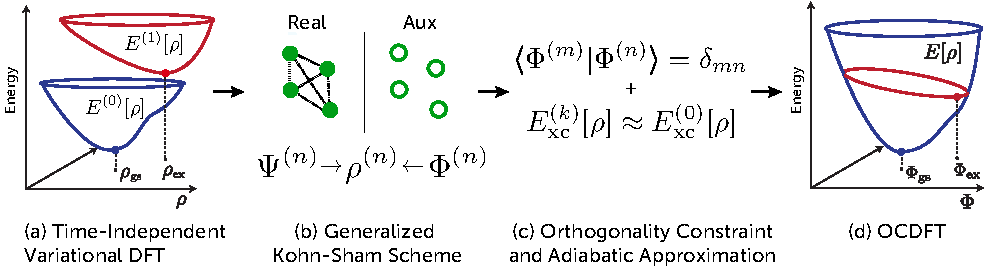
\includegraphics[width=6.5in]{figure_1.pdf}
\caption{Outline of Orthogonality Constrained DFT: (a) In the Ayers--Levy--Nagy time-independent variational formulation of DFT each electronic is associated with a unique density functional. (b) For each electronic state $\Psi^{(n)}$, an auxiliary system of non-interacting electrons with wave function $\Phi^{(n)}$ is introduced.   $\Psi^{(n)}$ and $\Phi^{(n)}$ are assumed to have the same electron density $\rho^{(n)}$. (c) We then impose explicit orthogonality conditions onto the auxiliary wave functions and approximate the unknown exchange-correlation (xc) functional $E_{\rm xc}^{(n)}$ with the ground-state functional. (d) The final OCDFT functional consists in the ground state functional augmented with an orthogonality constraint.}
\label{fig: OCDFTderiv}
\end{figure*}

%Defining a generalized Kohn--Sham system, we introduce 
As illustrated in Figure~\ref{fig: OCDFTderiv}, OCDFT invokes an adiabatic approximation similar to the one adopted in TDDFT, in which the xc contribution for each excited state is approximated by the ground state functional $E^{(0)}_{\rm xc}$. This results in the OCDFT functional for excited state $n$, which is given by:
\begin{equation}
\begin{split}
E^{(n)}_{\rm OCDFT}[\{\phi^{(n)}_i\}] =& - \frac{1}{2} \sum^{\rm occ}_i \langle \phi^{(n)}_i| \nabla^2 |\phi^{(n)}_i \rangle \\
 &+ \int d\textbf{r} \;  v_{\text{ext}}(\textbf{r}) \rho(\textbf{r}) \\
&+  E_{\text{Coul}}[\rho^{(n)}] + E^{(0)}_{\text{xc}}[\rho^{(n)}]
\label{eq:OCDFT_E_ORIGINAL}
\end{split}
\end{equation}
where $v_{\text{ext}}(\textbf{r})$ is the external potential and $E_{\text{Coul}}[\rho^{(n)}]$ is the classical electron-electron interaction energy term.

In this work we solve the OCDFT equations via our constrained multiple hole/particle (CMHP) algorithm.\cite{Wallace-OCDFT}
Within the CMHP scheme, each excited state is characterized by a pair of hole ($\phi_{\rm h}^n$) and particle ($\phi_{\rm p}^n$) orbitals, which are required to span the occupied and virtual space of the ground state wave function, respectively.  These may be interpreted as the orbitals from which an electron is annihilated and created as a result of an electronic excitation.
Rather than solving for the minimum orthogonality conditions between the states, the CMHP algorithm exploits the locality of hole orbitals in core-excited states by imposing sufficient \textit{orbital orthogonality conditions}. This approximation simplifies the Lagrangian, producing a computationally feasible minimization procedure.
In addition, it allows us to readily compute multiple excited states by enforcing mutual orthogonality conditions between the hole and particle orbitals of each subsequent excited state.
At the same time, the CMHP scheme fully accounts for relaxation of the remaining spectator orbitals. 

\subsection{Comparison of OCDFT and TDDFT for Core Excitations}
We have previously shown that OCDFT yields core excitation energies that are in better agreement with experiment than TDDFT.\cite{Wallace-OCDFT}
Specifically, we find that OCDFT excitation energies either do not require shifting, or if an energy shift is necessary, it is significantly smaller than the typical values used in TDDFT.
In this section we address the following questions:
1) Why do TDDFT core-excitation spectra require larger energy shifts than OCDFT?
and, 2) How much do \textit{shifted} TDDFT and OCDFT core-excitation spectra differ?

To showcase the differences between TDDFT and OCDFT, we computed the carbon and oxygen K-edge spectra of CO using a series of functionals with increasing amount of Hartree--Fock exchange.
For comparison, we also include results from time-dependent Hartree--Fock (TDHF) and orthogonality-constrained Hartree--Fock (OCHF).
In this example, we will not consider the effect of relativity since for C and O these contribute to shifts in the excitation energies of the order of 0.1--0.3 eV (see Section~\ref{sec:calibration}).
We will denote the fraction of Hartree--Fock exchange included in a functional with the letter $\delta$, and for simplicity we exclude range-corrected functionals from our analysis.

Figure~\ref{fig: C1s} shows the relative peak positions of the OCDFT and TDDFT spectra and the corresponding energy shift necessary to match the C$_{1\text{s} \rightarrow \pi^*}$ and O$_{1\text{s} \rightarrow \pi^*}$ peaks with their experimental values (287.40 and 534.10 eV for C and O, respectively).  See the supplementary material for a table with the data used to create this figure.
Note that for TDDFT, the C spectrum energy shift ranges from $-$6.96 (TDHF, $\delta = 1$) to +16.24 eV (BLYP, $\delta = 0$), while the O spectrum energy shift spans an even wider range (from $-$15.95 to +21.97 eV).
In comparison, OCDFT shifts are smaller, and range from $+$0.25 eV (OCHF) to +0.99 eV (BLYP) for carbon, and from $+$0.87 eV (BHLYP) to +1.77 eV (OCHF) for oxygen.


Figure~\ref{fig: C1s} also shows the relative position of the second, third, and fourth peaks of the K-edge spectrum.
In TDDFT, the position of these three transitions is heavily dependent on the amount of Hartree--Fock exchange.
In accordance with previous studies,\cite{Besly-57p} we note that only a functional with a large fraction of Hartree--Fock exchange like BHLYP ($\delta = 0.5$) can yield TDDFT relative excitation energies that are in sufficient agreement with experiment.
This does not seem to be the case for OCDFT.  Indeed, OCDFT relative peak positions are mostly insensitive to the choice of the functional being used, and surprisingly, both functionals with no (BLYP) and 100\% (HF) Hartree--Fock exchange yield C and O K-edge spectra that are in good agreement with the experimental spectra.
Overall, this example shows that there are fundamental differences between core excitation energies predicted by TDDFT and OCDFT.
%In addition to differences in the peak positions, there will also be differences in the predicted oscillator strengths.
In addition, there will also be differences in the oscillator strengths predicted by TDDFT and OCDFT. 
\begin{figure*}[h!]
	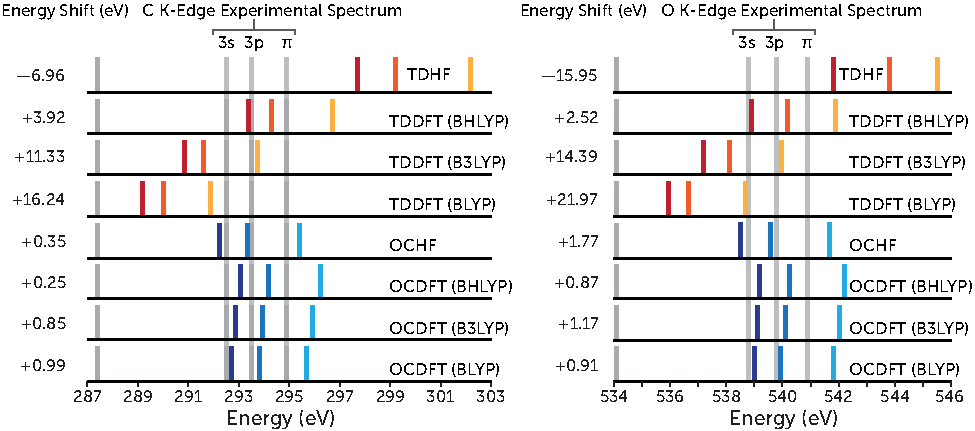
\includegraphics[width=6.5in]{figure_2.pdf}
	\caption{Relative Peak Positions of the C (left) and O (right) K-edge spectra of CO.
	Spectra are shifted by the amount required to align the first peak to the experimental peak values (287.40 and 534.10 eV for the C and O spectrum respectively).  All calculations use the aug-cc-pVQZ basis set.}
	\label{fig: C1s}
\end{figure*}

To understand the differences between TDDFT and OCDFT we analyze a model that captures the essential features of core-excited states.
The model used here is similar to that considered by Casida et al.\cite{Casida-TDDFT-CT-problem} and by Ziegler et al. \cite{Zeigler-TDDFT-CT-problem}.
We consider a system with three orbitals ($\phi_i$ , $\phi_a$, $\phi_b$) of different spatial symmetry.  The ground state of the model is assumed to be the closed-shell determinant $\ket{(\phi_i)^2}$, so that $\phi_a$ and $\phi_b$ are unoccupied orbitals.
We model K-edge transitions as ``charge-transfer-like'' states, that is we assume that the core orbital $\phi_i$ has negligible spatial overlap with virtual orbitals.  This assumption translates in to the condition $\int d\mathbf{r} |\phi_i(\mathbf{r})|^2 |\phi_p(\mathbf{r})|^2 = 0$ for $\phi_p$ equal to $\phi_a$ or $\phi_b$.

We consider the singlet core excitation energies for the transitions $\phi_i \rightarrow \phi_a$ ($\omega_{ai}$) and $\phi_i \rightarrow \phi_b$ ($\omega_{bi}$), together with the relative excitation energy $\Delta \omega = \omega_{bi} - \omega_{ai}$.
For this model, these excitation energies can be written down explicitly in terms of molecular integrals.\cite{Casida-TDDFT-CT-problem,Zeigler-TDDFT-CT-problem}
The reference excitation energies for our model are computed using CIS and are reported in Table \ref{table:OCDFT-CIS-TDDFT}.
In addition, we report the same quantities as obtained from TDDFT using the Tamm--Dancoff approximation and OCDFT with the exchange-correlation functional approximated as a Taylor expansion around the ground state density.
We refer the reader to Table \ref{table:OCDFT-CIS-TDDFT} for the definition of the integrals used in this section.

\begin{table*}[t!]
%	\center
	\caption{Singlet Excitation Energies for a Toy Model of Two Electrons in Three Molecular Orbitals.}
	\begin{tabular}{ll}
		\toprule
Method & Singlet excitation energy$^{a}$ \\
\midrule\\[-8pt]
CIS &   
 $\omega_{ai}^{\rm{CIS}} = h_a - h_i + J_{ai}-J_{ii}$ \\[6pt]
&$ \Delta \omega^{\rm{CIS}}= \omega_{bi} - \omega_{ai} = h_b-h_a  + J_{bi}- J_{ai}$ \\
\midrule
TDDFT 
&$\displaystyle\omega_{ai}^{\rm{TDDFT}} = \omega_{ai}^{\text{CIS}} 
+ (1-\delta) \left(v^{\text{x}}_{a} - v^{\text{x}}_{i} + J_{ai} -  J_{ii} \right)$\\[6pt] 
&$\displaystyle\Delta \omega^{\rm{TDDFT}} = \Delta\omega^{\text{CIS}} + (1-\delta) \left(v^{\text{x}}_{b}
-v^{\text{x}}_{a} + J_{bi} -  J_{ai}\right)$\\  
 \midrule
OCDFT 
& $\displaystyle\omega_{ai}^{\rm{OCDFT}}  = \omega^{\text{CIS}}_{ai} + (1-\delta)\left(v^{\text{x}}_{a}
  -v^{\text{x}}_{i} + \frac{1}{2} J_{aa} - \frac{1}{2} J_{ii}  
  +  \frac{1}{2} f^{\rm x}_{aa} +  \frac{1}{2} f^{\rm x}_{ii} \right)$\\[12pt] 
&$\displaystyle\Delta \omega^{\text{OCDFT}} = \Delta\omega^{\text{CIS}} +
(1-\delta)\left(v^{\text{x}}_{b}
-v^{\text{x}}_{a} + \frac{1}{2}J_{bb} -  \frac{1}{2} J_{aa}
+  \frac{1}{2} f^{\rm x}_{aa}- \frac{1}{2} f^{\rm x}_{bb}\right)$ \\
\bottomrule\\
\multicolumn{2}{l}{
\begin{minipage}{5in}%
\small
{$^a$}The ground state wave function is given by $|\Phi \rangle = | (\phi_i)^2\rangle$. All energies are expressed in terms of one-particle energies, $h_p=\langle\phi_p|\hat{h}|\phi_p\rangle$, density functional exchange potential $v^{\text x}_p = \langle \phi_p|v_{\text{x}}|\phi_p\rangle$, Coulomb $J_{pq}=(pp|r_{12}^{-1}|qq)$, and exchange kernel $f^{\rm x}_{pp} = (pp|f^{\alpha\alpha}_x|pp)$ integrals. The excitation energy of OCDFT is computed by a second-order expansion of the exchange-correlation functional around the ground state density. All contributions arising  from the correlation functional were neglected and minimum overlap between involved orbital is assumed $(\langle|\phi_a|^2 ||\phi_i|^2\rangle\sim 0 )$. The amount of Hartree--Fock exchange included in the density functional is indicated with $\delta \in [0,1]$.
\end{minipage}%
}
\end{tabular} \\

	\label{table:OCDFT-CIS-TDDFT}
\end{table*}

The origin of the large energy shift required to match TDDFT K-edge spectra with experiment may be traced down to the difference between the TDDFT and CIS excitation energy:
\begin{equation} \label{eq:tddft_error}
\omega_{ai}^{\rm{TDDFT}} - \omega_{ai}^{\text{CIS}} = (1-\delta) \left(v^{\text{x}}_{a} -v^{\text{x}}_{i} + J_{ai} -  J_{ii}\right).
\end{equation}
In the local density approximation (LDA), the exchange potential is equal to $v^{\rm x}[\rho] = - \frac{4}{3} C_x \rho^{1/3}$, where $C_x$ is a positive constant.
Therefore, we estimate that the matrix element $v^{\rm x}_{p} = \langle \phi_p|v_{\text{x}}|\phi_p\rangle$ will be larger for orbitals localized near regions with high electron density (i.e. atomic nuclei).  
As a consequence, for core excitations the term $v^{\rm x}_{a} -v^{\rm x}_{i}$ will be positive.
Indeed, for the lowest K-edge transition of CO we estimate this quantity from the full exchange-correlation potential as $v^{\rm xc}_{a} -v^{\rm xc}_{i}$, and find that it is about +48.4 eV for C and +70.9 eV for O.

Let us now turn to the contribution from the second term in Eq~\eqref{eq:tddft_error}, $J_{ai} -  J_{ii}$.
This term can be interpreted physically as the sum of the energy released from breaking the core electron pair ($-J_{ii}$) and the interaction of the unpaired electrons in the hole and particle orbitals ($J_{ai}$).
This term is already present with the correct prefactor in the CIS expression for the excitation energy ($\omega_{ai}^{\rm{CIS}}$), therefore, in the case of TDDFT it is double counted.
For core excitations one has that $J_{ii} \gg J_{ai}$.  Therefore, the second term in Eq~\eqref{eq:tddft_error} is negative, and has the net effect of shifting down the excitation energies.
Since TDDFT core excitation energies are always underestimated, we expect that $J_{ai} -  J_{ii}$ is larger in magnitude than the term $v^{\rm x}_{a} -v^{\rm x}_{i}$.
Indeed, in the case of the lowest energy transition, we find that $J_{ai} -  J_{ii}$ is respectively $-89.7$ and $-123.4$ eV for the C and O K-edge.
Combining these estimates with those for the exchange contributions, we predict TDDFT energy shifts of the order of $-41.4$ eV for C and $-52.1$ eV for O.
These estimates do not agree well with the TDDFT actual shifts, but they still capture some of the essential features of our data for CO: 1) they predict negative shifts that are dominate by the two-electron repulsion contribution, and 2) they predict that the oxygen energy shift is larger in magnitude than that required for carbon.
Note that this model predicts that as the percentage of Hartree--Fock exchange is increased ($\delta \rightarrow 1$), the TDDFT core excitation energies require less shifting.
This observation is in agreement with numerical results.
Indeed, one way to improve the accuracy of TDDFT for core excitation energies is to use functionals with a relatively high fraction of Hartree--Fock exchange (50--60\%).\cite{Besly-57p}

In the case of OCDFT, the equation for the energy shift differs from that of TDDFT and it is somewhat more difficult to analyze.
In addition to a term proportional to $v^{\rm x}_{a} -v^{\rm x}_{i}$, which is also common to the TDDFT expression, the OCDFT shift has various contributions from several local self-interaction terms.
Focusing on the contribution from the two-electron interactions, $\frac{1}{2}(J_{aa} - J_{ii})$, this quantity is equal to $-61.9$ and $-45.0$ eV for O and C, respectively.
In comparison to the TDDFT two-electron contribution, the magnitude of this term is smaller and there is better cancellation of errors.

Turning to our second question, we use the three-state model to compute the relative excitation energies for both the TDDFT and OCDFT spectra.
The excitation energy difference  between the two single excitations as predicted by TDDFT ($\Delta \omega^{\rm{TDDFT}} = \omega_{bi}^{\rm{TDDFT}} - \omega_{ai}^{\rm{TDDFT}}$) differs from the CIS value by the quantity $(1-\delta) \left(v^{\text{x}}_{b}-v^{\text{x}}_{a} + J_{bi} -  J_{ai}\right)$.
The most worrisome contribution to the error is the difference $J_{bi} -  J_{ai}$, which effectively introduces a distance dependence in the excitation energy error.

In the case of OCDFT, the relative excitation energy differs from the CIS value by a combination of exchange potential integrals ($v_b^x - v_a^x$, which also contributes to the TDDFT error) and a sum of differences of self-interaction energies for orbitals $\phi_a$ and $\phi_b$.
Thus, all the terms that contribute to the OCDFT relative energy error are local, and relative excitation energies should not show a marked dependence on the distance between the hole and particle orbitals.

\section{Computational Details}
Core excitation energies are computed with OCDFT using the nonrelativistic Hamiltonian, the spin-free X2C Hamiltonian, and the second-, third-, and fourth-order variants of the DKH (DKH2--4) Hamiltonian. Benchmark core excitation energies were computed for 13 small molecules (CH$_4$, C$_2$H$_4$, HCN, CO, H$_2$CO, N$_2$, N$_2$O,
 SO$_2$, SiH$_4$, PH$_3$, H$_2$S, HCl, Cl$_2$).
The geometries of the test set molecules were optimized with nonrelativistic DFT using Becke's B3LYP \cite{becke_new_1993,lee_development_1988,vosko_accurate_1980,stephens_ab_1994} exchange-correlation functional and the def2-QZVP \cite{weigend_balanced_2005,weigend_accurate_2006} basis set. Individual excitation energies are compared with data obtained from gas-phase NEXAS experiments\cite{puttner_vibrationally_1999,remmers_high-resolution_1992,CO-expt-Kedge,chen_k-shell_1989,tronc_nitrogen_1980,tronc_carbon_1979,francis_studies_1994,adachi_vibronic_1999,hitchcock_k-shell_1979,domke_carbon_1990,nayandin_angle-resolved_2001,bodeur_single-and_1990,gedat_s_1998,hudson_high-resolution_1994,cavell_chemical_1999,bodeur_photoabsorption_1985}.

Geometries for the three titanium complexes used in the study are taken from ref.\citenum{TiCl4} and \citenum{TiCl4-Zeigler}.  The first is a simple tetrahedral TiCl$_4$ complex, while the other two are the mono- and bis-cyclopentadienyl (Cp) complexes TiCpCl$_3$ and TiCp$_2$Cl$_2$. The geometries used in our computations show only small deviations from crystal structures (changes of less than 0.02 $\AA$ in bond length and 0.5$^{\circ}$ in bond angle). OCDFT results for titanium complexes are obtained with the fully uncontracted cc-pVDZ\cite{cc-pvdz-dk-Al-Ar,cc-pvdz-dk-H-Ne} (un-cc-pVDZ) basis set with the two-electron integrals approximated using a density fitting approximation\cite{DF-def2-TZVP-JK,DF-def2-TZVP-JK-1,BAERENDS197341,B000027M,DF-SABIN} with the def2-TZVP-JK auxiliary basis\cite{JCC20702}. For the test set, the fully uncontracted  aug-cc-pVDZ\cite{aug-cc-pvdz-B-F}  (un-aug-cc-pVDZ) basis set was used without the density fitting approximation.
Fully uncontracted basis sets are required to provide a proper description of the small component of the wave function and to guarantee a fair comparison between nonrelativistic and relativistic methods. For these organotitanium complexes, OCDFT core excitation energies are computed using only the X2C Hamiltonian.

 X2C-OCDFT calculations are performed with the \textsc{psi4} \textit{ab initio} quantum chemistry package\cite{PSI4} using our implementation of X2C in \textsc{psi4}.  DKH+OCDFT calculations are performed with \textsc{psi4} using the code of Reiher, Wolf, and Hess\cite{DKHn-Reiher,DKH}. All TD-DFT calculatons are done with the ORCA software package version 3.0.3\cite{ORCA}. Natural population analysis on the Ti complexes were performed using the \textsc{janpa}\cite{nikolaienko_janpa:_2014} software package.

\section{Results and Discussion}
\label{sec:calibration}
\subsection{Calibration of X2C-OCDFT Core Excitation Energies}
In order to gauge the importance of relativistic effects in OCDFT core excitation energies, nonrelativistic (NR) and relativistic computations are performed on a test set of 36 transitions from 13 molecules containing first- and second-row elements. 

\begin{table*}[t!]
\center
\caption{Excitation energies of the three lowest energy 1s core excitations for each atom in CO calculated with X2C-OCDFT using the B3LYP functional and fully uncontracted cc-pV$X$Z and aug-cc-pV$X$Z basis sets ($X$ = D, T, Q). Experimental values are taken from Refs. \citenum{CO-expt-Kedge} and \citenum{tronc_carbon_1979}. Errors greater than 1 eV are indicated with bold font.}
\begin{tabular}{ccrrrrrr}
\toprule
Transition & Exp. & \multicolumn{3}{c}{un-cc-pV$X$Z}& \multicolumn{3}{c}{un-aug-cc-pV$X$Z} \\ \cmidrule(r){3-5}  \cmidrule(l){6-8}
 & & D \space & T \space & Q \space & D \space & T \space & Q \space \\
\midrule
O$_{1\mathrm{s} \rightarrow \pi^*}$ & 534.1 & $-$0.4 & $-$0.8 & $-$0.9 & $-$0.4 & $-$0.8 & $-$0.9 \\
O$_{1\mathrm{s} \rightarrow 3\mathrm{s}}$ & 538.8 & \textbf{3.9} & \textbf{1.9} & 0.9 & 0.0 & $-$0.5 & $-$0.6 \\
O$_{1\mathrm{s} \rightarrow 3\mathrm{p}}$ & 539.8 & \textbf{7.8} & \textbf{4.1} & \textbf{2.4} & 0.1 & $-$0.5 & $-$0.6 \\
C$_{1\mathrm{s} \rightarrow \pi^*}$ & 287.4 & $-$0.5 & $-$0.8 & $-$0.8 & $-$0.5 & $-$0.8 & $-$0.9 \\
C$_{1\mathrm{s} \rightarrow 3\mathrm{s}}$ & 292.5 & \textbf{4.0} & \textbf{2.1} & \textbf{1.1} & 0.0 & $-$0.4 & $-$0.5 \\
C$_{1\mathrm{s} \rightarrow 3\mathrm{p}}$ & 293.4 & \textbf{7.1} & \textbf{4.0} & \textbf{2.4} & 0.3 & $-$0.2 & $-$0.3 \\[3pt]
MAE & & \textbf{4.0} & \textbf{2.3} & \textbf{1.4} & 0.2 & 0.5 & 0.6 \\ 
\bottomrule
\end{tabular}
\label{table:Basis}
\end{table*}

Table \ref{table:Basis} shows the systematic convergence of X2C-OCDFT on a test case of six core excitations of CO using the fully uncontracted correlation consistent cc-pV$X$Z and aug-cc-pV$X$Z series of basis sets ranging from double- to quadruple-$\zeta$ quality. Both 1s $\rightarrow$ $\pi^*$ excitations in CO are represented well across all the basis sets considered, with the addition of diffuse functions having no significant impact on the accuracy of the excitation energies compared to experiment. However, the cc-pV$X$Z series of basis sets struggle to properly describe the 1s $\rightarrow$ 3s and 1s $\rightarrow$ 3p transitions in CO, and the inclusion of diffuse functions drastically improves the accuracy of these excitation energies.
The un-aug-cc-pVDZ basis set provides a convenient compromise between accuracy and cost, and was chosen to benchmark the full test set of core excitations.

 \begin{figure}[!t]
 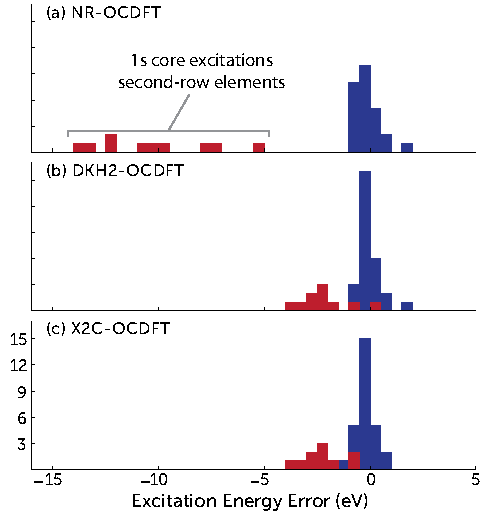
\includegraphics{figure_3.pdf}
 \caption{Error distribution in the computed core excited states for: (a) nonrelativistic OCDFT, (b) OCDFT with the second-order Douglas--Kroll--Hess Hamiltonian, and (c) OCDFT with the exact-2-component Hamiltonian. All calculations use the B3LYP functional and a fully uncontracted aug-cc-pVDZ basis set.  Red bars indicate core excitations from 1s orbitals of second-row elements.}
 \label{fig:histogram}
 \end{figure}

Table \ref{table:FirstRow} and \ref{table:SecondRow} report core excitations from first- and second-row elements.
The performance of OCDFT for \textit{first-row} core excitations is slightly improved upon inclusion of scalar relativistic effects.
Going from NR-OCDFT to OCDFT with scalar relativistic Hamiltonians (X2C, DKH2--4) reduces the error by about 0.2 eV.
In addition, the maximum absolute deviation between X2C-OCDFT and NR-OCDFT for first-row core excitations is only 0.4 eV (O$_{\text{1s}\rightarrow\text{3s}}$ transition of N$_2$O).
X2C and low-order DKH methods yield results that are identical, with negligible differences in MAE.
This similarity in performance between NR-OCDFT and multiple scalar relativistic Hamiltonians is consistent with the general observation that scalar relativistic effects are not significant for the core excitation energies of first row elements.\cite{Asmuruf2008267,Wallace-OCDFT,Besley-EOM-MOM}  A similar conclusion can be drawn from the second row 2$\text{p}$ excitation energies shown in the bottom half of Table \ref{table:SecondRow} where the difference in MAE between NR and relativistic OCDFT is negligible, with identical results produced across all orders of DKH. 

\begin{table*}[t!]
	\caption{OCDFT core excitation energies for molecules containing first-row elements using nonrelativistic (NR) and relativistic (X2C,DKH2, DKH3, DKH4) Hamiltonians. Computations were performed using the uncontracted aug-cc-pVDZ basis with the B3LYP exchange-correlation functional ($E^{\text{B3LYP}}_{\rm xc}$) and 100\% non-local exact exchange ($E^{\text{HF}}_{\rm x}$). OCDFT results are reported here as deviations from the experimental excitation energies (in eV).  The mean absolute error (MAE) is also reported for each method. Experimental values are taken from refs \citenum{puttner_vibrationally_1999,remmers_high-resolution_1992,CO-expt-Kedge,chen_k-shell_1989,tronc_nitrogen_1980,tronc_carbon_1979,francis_studies_1994,adachi_vibronic_1999,hitchcock_k-shell_1979,domke_carbon_1990}.}
\begin{tabular}{lllrrrrrr}
\toprule
Molecule & Excitation   & Exp.  & \multicolumn{6}{c}{Error} \\  \cmidrule(l){4-9}
&            &           &   \multicolumn{5}{c}{$E^{\text{B3LYP}}_{\rm xc}$} & $E^{\text{HF}}_{\rm x}$ \\ \cmidrule(l){4-8} 
&            &           &   NR &  ${\text{X2C}}$ & ${\text{DKH2}}$ & ${\text{DKH3}}$ & ${\text{DKH4}}$ & X2C \\
\midrule
CO 	 		& C$_{\text{1s}\rightarrow\pi^*}$ & 287.4 & $-$0.6 & $-$0.6 & $-$0.5 & $-$0.5 & $-$0.5 & 0.1 \\
			 & C$_{\text{1s}\rightarrow\text{3s}}$ & 292.4 & 0.0 & 0.0 & 0.1 & 0.1 & 0.1 & 0.0 \\
			 & O$_{\text{1s}\rightarrow\pi^*}$ & 534.2 & $-$0.9 & $-$0.5 & $-$0.5 & $-$0.5 & $-$0.5 & $-$1.1 \\
			 & O$_{\text{1s}\rightarrow\text{3s}}$ & 538.9 & $-$0.5 & $-$0.5 & $-$0.1 & $-$0.1 & $-$0.1 & $-$1.2 \\
H$_2$CO 	&  O$_{\text{1s}\rightarrow\pi^*}$ & 530.8 & $-$0.6 & $-$0.2 & $-$0.2 & $-$0.2 & $-$0.2 & $-$0.8 \\
		 & O$_{\text{1s}\rightarrow\text{3s}}$ & 535.4 & $-$0.5 & $-$0.2 & $-$0.2 & $-$0.2 & $-$0.2 & $-$1.3 \\
		& C$_{\text{1s}\rightarrow\text{3s}}$ & 290.2 & $-$0.3 & $-$0.2 & $-$0.2 & $-$0.2 & $-$0.2 & $-$0.6 \\
		 & C$_{\text{1s}\rightarrow\pi^*}$ & 286.0 & $-$0.4 & $-$0.3 & $-$0.3 & $-$0.3 & $-$0.3 & $-$0.2 \\
N$_2$O & O$_{\text{1s}\rightarrow\pi^*}$ & 534.8 & $-$0.5 & $-$0.2 & $-$0.1 & $-$0.1 & $-$0.1 & $-$1.3 \\
		 & O$_{\text{1s}\rightarrow\text{3s}}$ & 536.7 & $-$0.6 & $-$0.2 & $-$0.2 & $-$0.2 & $-$0.2 & $-$3.1 \\
		 & $^c$N$_{\text{1s}\rightarrow\text{3s}}$$^{a}$ & 407.5 & 0.2 & 0.3 & 0.3 & 0.3 & 0.3 & 39.2$^{b}$ \\
		 & $^t$N$_{\text{1s}\rightarrow\pi^*}$$^{a}$ & 401.1 & $-$0.8 & $-$0.5 & $-$0.6 & $-$0.6 & $-$0.6 & 10.4$^{b}$ \\
N$_2$	 & N$_{\text{1s}\rightarrow\pi^*}$ & 401.0 & $-$0.8 & $-$0.5 & $-$0.5 & $-$0.5 & $-$0.5 & 8.9$^{b}$ \\
HCN 	& C$_{\text{1s}\rightarrow\pi^*}$ & 286.4 & $-$0.3 & $-$0.2 & $-$0.2 & $-$0.2 & $-$0.2 & $-$0.3 \\
		 & C$_{\text{1s}\rightarrow\text{3s}}$ & 289.1 & $-$0.2 & $-$0.1 & $-$0.1 & $-$0.1 & $-$0.1 & $-$0.4 \\
		 & N$_{\text{1s}\rightarrow\pi^*}$ & 399.7 & $-$0.6 & $-$0.4 & $-$0.4 & $-$0.4 & $-$0.4 & $-$0.6 \\
		 & N$_{\text{1s}\rightarrow\text{3s}}$ & 401.8 & 0.2 & 0.4 & 0.4 & 0.4 & 0.4 & $-$1.0 \\
CH$_4$	   & C$_{\text{1s}\rightarrow\text{3p}}$ & 288.0 & $-$0.3 & $-$0.2 & $-$0.2 & $-$0.2 & $-$0.2 & $-$0.3 \\
           & C$_{\text{1s}\rightarrow\text{3s}}$ & 287.1 & $-$0.7 & $-$0.6 & $-$0.6 & $-$0.6 & $-$0.6 & $-$0.6 \\
C$_2$H$_2$ & C$_{\text{1s}\rightarrow\pi^*}$ & 285.8 & $-$0.5 & $-$0.3 & $-$0.4 & $-$0.4 & $-$0.4 & 7.6$^{b}$ \\[3pt]
MAE       & &  & 0.5  & 0.3 & 0.3 & 0.3 & 0.3 & 0.8 \\	
\bottomrule		
	\end{tabular}\\	
	$^{a}$The subscripts c and t stand for the center and tail nitrogen of N$_2$O, respectively.\\
	$^{b}$Excitation excluded from the computation of the MAE.
	\label{table:FirstRow}
\end{table*}

Figure \ref{fig:histogram} shows the distribution of errors for all the test set transitions computed with the NR, X2C, and DKH2 Hamiltonians.
Note how the 1s orbital (K-edge) transitions for second-row elements (shaded red in Figure \ref{fig:histogram}) are consistently underestimated by NR-OCDFT and yield a MAE of 10.3 eV.
These troublesome transitions are drastically improved with the inclusion of scalar relativistic effects, reducing the MAE down to 2.3 eV.
Even for excitations that involve second-row element we notice that the X2C and DKH2--4 methods are in excellent agreement (difference in energy less than 0.1 eV).

\begin{table*}[t!]
	\caption{OCDFT core excitation energies for molecules containing first-row elements using nonrelativistic (NR) and relativistic (X2C,DKH2, DKH3, DKH4) Hamiltonians. Computations were performed using the uncontracted aug-cc-pVDZ basis with the B3LYP exchange-correlation functional ($E^{\text{B3LYP}}_{\rm xc}$) and 100\% non-local exact exchange ($E^{\text{HF}}_{\rm x}$). OCDFT results are reported here as deviations from the experimental excitation energies (in eV).  The mean absolute error (MAE) is also reported for each method.
Experimental values are from refs \citenum{nayandin_angle-resolved_2001,bodeur_single-and_1990,gedat_s_1998,hudson_high-resolution_1994,cavell_chemical_1999,bodeur_photoabsorption_1985}}
	\centering
	\begin{tabular}{llrrrrrrr}
\toprule
Molecule & Excitation   & Exp.  & \multicolumn{6}{c}{Error} \\  \cmidrule(l){4-9}
&            &           &   \multicolumn{5}{c}{$E^{\text{B3LYP}}_{\rm xc}$} & $E^{\text{HF}}_{\rm x}$ \\ \cmidrule(l){4-8} 
&            &           &   NR &  ${\text{X2C}}$ & ${\text{DKH2}}$ & ${\text{DKH3}}$ & ${\text{DKH4}}$ & X2C \\
\midrule
SiH$_4$ & Si$_{\text{1s}\rightarrow\sigma^*}$ & 1842.5 & $-$5.3 & $-$1.0 & $-$1.0 & $-$1.0 & $-$1.0 & 1.6 \\
PH$_3$ & P$_{\text{1s}\rightarrow\sigma^*}$ & 2145.8 & $-$7.6 & $-$1.8 & $-$1.8 & $-$1.8 & $-$1.8 & 1.2 \\
H$_2$S & S$_{\text{1s}\rightarrow\sigma^*}$ & 2473.1 & $-$10.5 & $-$2.8 & $-$2.8 & $-$2.8 & $-$2.8 & 0.7 \\
 & S$_{\text{1s}\rightarrow\text{4p}}$ & 2476.3 & $-$9.9 & $-$2.2 & $-$2.2 & $-$2.2 & $-$2.2 & 0.8 \\
SO$_2$ & S$_{\text{1s}\rightarrow\pi^*}$ & 2473.8 & $-$10.6 & $-$2.9 & $-$2.9 & $-$2.9 & $-$2.9 & 0.5 \\
 & S$_{\text{1s}\rightarrow\text{4p}}$ & 2478.4 & $-$7.3 & $-$0.8 & 0.4 & 0.4 & 0.4 & 3.7 \\
HCl & Cl$_{\text{1s}\rightarrow\sigma^*}$ & 2823.9 & $-$13.2 & $-$3.2 & $-$3.2 & $-$3.2 & $-$3.2 & 0.4 \\
 & Cl$_{\text{1s}\rightarrow\text{4p}}$ & 2827.8 & $-$12.2 & $-$2.2 & $-$2.2 & $-$2.2 & $-$2.2 & 1.1 \\
Cl$_2$ & Cl$_{\text{1s}\rightarrow\sigma^*}$ & 2821.3 & $-$13.6 & $-$3.6 & $-$3.6 & $-$3.6 & $-$3.6 & 16.8$^{a}$ \\
& Cl$_{\text{1s}\rightarrow\text{4p}}$ & 2828.5 & $-$12.4 & $-$2.3 & $-$2.4 & $-$2.3 & $-$2.3 & 18.0$^{a}$ \\[3pt]
MAE  & & &  10.3 & 2.3 & 2.3 & 2.2 & 2.2 & 1.3\\
\midrule
SiH$_4$ & Si$_{\text{2p}\rightarrow\sigma^*}$ & 102.8 & 0.9 & 0.9 & 0.9 & 0.9 & 0.9 & 1.2 \\
PH$_3$ & P$_{\text{2p}\rightarrow\sigma^*}$ & 132.3 & 0.3 & 0.3 & 0.3 & 0.3 & 0.3 & 0.6 \\
H$_2$S & S$_{\text{2p}\rightarrow\sigma^*}$ & 164.5 & 0.7 & 0.7 & 0.7 & 0.7 & 0.7 & 1.8 \\
H$_2$S & S$_{\text{2p}\rightarrow\text{4s}}$ & 166.5 & 1.6 & $-$1.5 & 1.6 & 1.6 & 1.6 & 1.8 \\
Cl$_2$ & Cl$_{\text{2p}\rightarrow\sigma^*}$ & 198.7 & $-$0.5 & $-$0.5 & $-$0.5 & 0.0 & 0.0 & $-$0.1 \\
HCl & Cl$_{\text{2p}\rightarrow\text{4s}}$ & 201.0 & 0.3 & 0.3 & 0.3 & 0.6 & 0.3 & 1.3 \\[3 pt]
MAE & & & 0.7 & 0.7& 0.7 & 0.7 & 0.6 & 1.1 \\
\bottomrule
\end{tabular}\\
$^{a}$Excitation excluded from the computation of the MAE.
\label{table:SecondRow}
\end{table*} 

In order to test the importance of correlation effects for the computation of core excitation energies, OCDFT was applied to the test set using a functional with 100\% non-local exchange ($E^{\text{HF}}_{\rm x}$). These results are displayed in the far right-hand column of Tables \ref{table:FirstRow} and \ref{table:SecondRow}.
It is important to notice that for transitions in molecules with equivalent or near-equivalent nuclei (C$_2$H$_2$, N$_2$O, N$_2$, Cl$_2$), we previously determined that it is necessary to seek a wave function with hole orbitals localized on one atom.\cite{Wallace-OCDFT} Broken symmetry calculations were used in order to obtain OCDFT excitation energies of C$_2$H$_2$, N$_2$, N$_2$O and Cl$_2$. However, we were unable to obtain localized hole orbitals for these molecules with OCDFT and the $E^{\text{HF}}_{\rm x}$ functional.
When transitions with delocalized hole orbitals are excluded, the HF functional provides results that are in modest agreement with those obtained using the B3LYP functional. For the first row elements the maximum difference observed in Table \ref{table:FirstRow} between $E^{\text{HF}}_{\rm x}$ and $E^{\text{B3LYP}}_{\rm xc}$ is 2.9 eV (N$_2$O, O$_{1\text{s} \rightarrow 3\text{s}}$ transition), while for second row elements the corresponding largest difference observed in Table \ref{table:SecondRow} is 4.5 eV (SO$_2$, S$_{1\text{s} \rightarrow 4\text{p}}$ transition).

Table \ref{table:CorrRel} reports estimates of relativistic and correlation effects.  The former are computed as the difference between the NR- and X2C-OCDFT excitation energies, while the latter are estimated as the difference between the relativistic results using the B3LYP and Hartree--Fock exchange.
The results in Table \ref{table:CorrRel} show that relativistic and correlation effects follow the trend: 1s first-row < 2p second-row < 1s second row.  For first row 1$\text{s}$ and second row 2$\text{p}$ excitations, correlation effects are larger than relativistic effects; this trend reverses in the second row 1$\text{s}$ excitations.

\begin{table}[t!]
\caption{Importance of relativistic and correlation effects in core excitations computed with X2C-OCDFT.  Relativistic effects are estimated as the difference between NR and X2C OCDFT calculations [OCDFT$^{\rm NR}$(E$^{\text{B3LYP}}_{\rm xc}$) $-$ OCDFT$^{\rm X2C}$(E$^{\text{B3LYP}}_{\rm xc}$)], while correlation effects are estimated as the difference between B3LYP and HF OCDFT calculations [OCDFT$^{\rm X2C}$(E$^{\text{B3LYP}}_{\rm xc}$) $-$ OCDFT$^{\rm X2C}$(E$^{\text{HF}}_{\rm x}$)]. Molecules with symmetry equivalent nuclei were excluded from this analysis due to inability of the HF functional to obtain a broken-symmetry solution (see text for further details).}
\begin{tabular}{ccc}
\toprule
Transitions & Relativistic (eV) & Correlation (eV) \\
\midrule
First row 1s & 0.2 & 0.6 \\
Second row 1s & 8.0 & 3.4 \\
Second row 2p & 0.5 & 1.1 \\
All & 2.2 & 1.3 \\
\bottomrule
\end{tabular}
\label{table:CorrRel}
\end{table}

\subsection{Ti K-Edge NEXAS of Organotitanium Complexes}
In this section we will apply the X2C-OCDFT approach to compute the Ti K-edge spectrum of TiCl$_4$ and its mono- and bis-cyclopentadienyl derivatives, TiCpCl$_3$ and TiCp$_2$Cl$_2$.
These compounds have drawn ample attention due to their catalytic activity and potential use as anticancer drugs.
The increased contribution of relativistic effects in the Ti core and the closed shell electronic configuration (d$^0$) of tetracoordinated Ti complexes makes these molecules an ideal test case for investigating the role of relativistic effects on the computation of NEXAS spectra. 
DeBeer et al.\cite{TiCl4} obtained the experimental NEXAS spectra of TiCl$_4$, TiCpCl$_3$, and TiCp$_2$Cl$_2$, and explained peak positions and intensities using ground state nonrelativistic DFT calculations. Ziegler and co-workers\cite{TiCl4-Zeigler} studied this class of Ti complexes, employing a relativistic TDDFT approach that made use of the two-component scaled ZORA variant\cite{ZORA-fix-energy-scale}. While the ZORA-TDDFT spectra displayed excellent qualitative agreement with experimental features\cite{TiCl4}, core excitation energies were underestimated by about 18 eV. 

\begin{table}[!t]
%\small
\caption{TiCl$_4$ pre-edge excitation energies computed with TDDFT and OCDFT using nonrelativistic (NR) and relativistic (DKH2,X2C) Hamiltonians.
Results are reported as deviations from the experimental peak maximum (in eV, from ref \citenum{TiCl4}).
All calculations use the B3LYP functional and the uncontracted cc-pVDZ basis set.}
\begin{tabular}{cccccc}
\toprule
State & \multicolumn{2}{c}{TDDFT} & \multicolumn{2}{c}{OCDFT} & Exp. \\ \cmidrule(r){2-3}  \cmidrule(l){4-5}
 & NR & DKH2 & NR & X2C  \\
\midrule
1 & $-$107.9& $-$78.6& $-$35.6& $-$5.0 & \multirow{5}{*}{$\left. \vphantom{\begin{tabular}{c}3\\3\\3 \\3\end{tabular}}\right\}$ 4969.2} \\
2 & $-$107.9& $-$78.6& $-$35.5& $-$4.5 \\
3 & $-$107.0& $-$77.6& $-$36.4& $-$5.7 \\
4 & $-$106.9& $-$77.6& $-$35.3& $-$4.8 \\
5 & $-$107.0& $-$77.7& $-$36.3& $-$5.7 \\
\bottomrule
	\label{table:Ti-complex}
\end{tabular}
\end{table}

In this work we focus on the analysis of the Ti K-edge spectrum of the three organotitanium compounds.
Table \ref{table:Ti-complex} reports the pre-edge excitations of TiCl$_4$ computed with OCDFT and TDDFT using nonrelativistic and relativistic Hamiltonians.
These results highlight the significant difference in accuracy between the OCDFT and TDDFT Ti K-edge excitation energies.
For example, Ti 1s core excitation energies computed at the nonrelativistic TDDFT level of theory are underestimated, on average, by 107.3 eV compared to the experimental peak position. The addition of scalar relativistic effects via the DKH2 Hamiltonian reduces the TDDFT error to 78.0 eV, which is still a significant deviation from experiment. Nonrelativistic OCDFT core excitation energies underestimate the experimental results by 35.8 eV. Inclusion of scalar relativistic effects via the X2C Hamiltonian reduces this error to 5.1 eV, showing much better agreement with the experimental pre-edge position (4969.2 eV).
Note that since we do not have access to a X2C-TDDFT implementation our results are based on the DKH2 Hamiltonian.  The comparison between X2C and DKH2 results is justified by the fact that these two method yield almost identical excitation energies for the test sets.  Moreover, both DKH2 and X2C shift the Ti core excitation energy by ca. 30 eV.

\begin{figure}[t!]
	\centering
	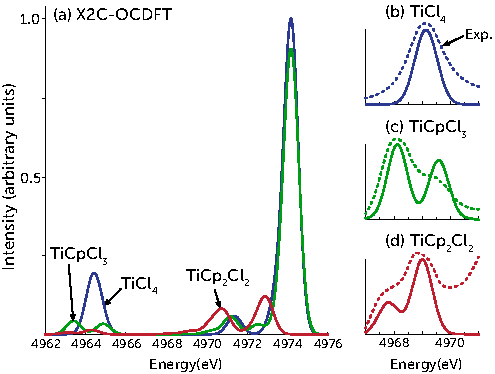
\includegraphics{figure_4.pdf}
	\caption{(a) Near-edge X-ray absorption spectrum of TiCl$_4$, TiCpCl$_3$, and TiCp$_2$Cl$_2$ computed with X2C-OCDFT at the B3LYP/un-cc-pVDZ level of theory.  (b)--(d) Comparison of the onset of the pre-edge experimental spectra (dotted line) with the X2C-OCDFT spectrum shifted by +4.7 eV to match the experimental pre-edge peak of TiCl$_4$ (solid line). Experimental curves taken from ref \citenum{TiCl4}. Ti K-edge for each molecule was simulated using 25 unique core-excited state (see supplementary material to see all excited states).}
	\label{fig:Ti-spectra}
\end{figure}

The unshifted X2C-OCDFT Ti K-edge peaks of TiCl$_4$, TiCpCl$_3$, and TiCp$_2$Cl$_2$ are reported in Table~\ref{table:pre-edge}, while Figure \ref{fig:Ti-spectra} shows a theoretical spectra simulated using 25 core excited states, together with a comparison of the shifted spectra with the experimental pre-edge features.\cite{TiCl4}
In accordance with experiment\cite{TiCl4}, X2C-OCDFT predicts the most intense absorption for TiCl$_4$ while the least intense for TiCp$_2$Cl$_2$. The relative ordering of the excitation energies of the three complexes predicated by OCDFT is in agreement with experiment as well. The most intense pre-edge feature for TiCl$_4$ occurs at 4964.4 eV (Expt. 4969.2 eV), while for TiCpCl$_3$, and TiCp$_2$Cl$_2$ it occurs at 4964.9 (Expt. 4968.1 eV) and 4964.3 (Expt. 4967.3) eV respectively.
It is also worth noting that the magnitude of the peak splitting is represented well by OCDFT. Our calculated pre-edge peaks for TiCpCl$_3$ and TiCp$_2$Cl$_2$ are split by 1.4 eV and 1.2 eV respectively, which are in excellent agreement with the experimental splitting of 1.4 eV observed for both compounds.

 \begin{table}[!b]
\caption{Transition energies (in eV) and relative oscillator strengths ($f$) for pre-edge transitions of TiCl$_4$, TiCpCl$_3$, and TiCp$_2$Cl$_2$ computed with X2C-OCDFT at the B3LYP/un-cc-pVDZ level of theory. Oscillator strengths shown are values relative to the most intense Ti K-edge transition of these three compounds (see supplementary material for detail).}
\begin{tabular}{ccccccc}
\toprule
State &   \multicolumn{2}{c}{\textbf{TiCl$_4$}}   & \multicolumn{2}{c}{\textbf{TiCpCl$_3$}} & \multicolumn{2}{c}{\textbf{TiCp$_2$Cl$_2$}} \\
& Energy & $f$ & Energy  & $f$ & Energy  & $f$ \\
     \cmidrule(r){2-3} \cmidrule(lr){4-5} \cmidrule(lr){6-7}  
1     &   4964.2 &             0.0945   & 4963.4 &    0.0202   & 4963.1 &                              0.0078 \\
2     &   4964.7 &             0.0940   & 4963.4 &    0.0191   &  4964.3 &                              0.0121 \\
3     &   4963.5 &             0.0002   & 4963.5 &    0.0164   & 4964.4 &                              0.0009 \\
4     &  4964.4  &             0.0947   &  4964.9 &   0.0220  & 4964.4 &                              0.0000 \\
5      & 4963.5         &      0.0000    & 4964.9 &   0.0217   & 4964.3 &                              0.0055 \\
\bottomrule
 	\end{tabular}
 	\label{table:pre-edge}
 \end{table}

The splitting of the pre-edge peak in the Cp-substituted compounds can be easily understood by examining the hole and particle orbitals that characterize each transition.
Figure \ref{fig:Ti-MOs} shows the particle orbitals for the five lowest excited states grouped according to which pre-edge feature they contribute.
In TiCl$_4$ all of the particle orbitals are combinations of Ti 3d, Ti 4p, and Cl 3p orbitals.
However, upon replacement of Cl with Cp ligands, the particle orbitals split into a group with no Cp ligand contribution (low energy) and a group with significant Cp ligand contribution (high energy).
Our assignment of the pre-edge peaks of TiCl$_4$ and TiCpCl$_3$ is in agreement with that of Ziegler et al.\cite{TiCl4-Zeigler}
However, our assignment of the Ti K-edge of TiCp$_2$Cl$_2$ is slightly different from the one reported by Ziegler\cite{TiCl4-Zeigler} and DeBeer.\cite{TiCl4}
Our OCDFT results suggest that the low energy peak is the result of a single transition while the second peak is a result of two transitions.
OCDFT predicts that these three peaks have similar intensities, which results in the 1:2 ratio of the absorption profile.
Ziegler et al.\cite{TiCl4-Zeigler} instead find that each peak in the K-edge of TiCp$_2$Cl$_2$ is due to a single transition, with the second transition being twice as intense as the first one.

\begin{figure*}[t!]
	\centering
	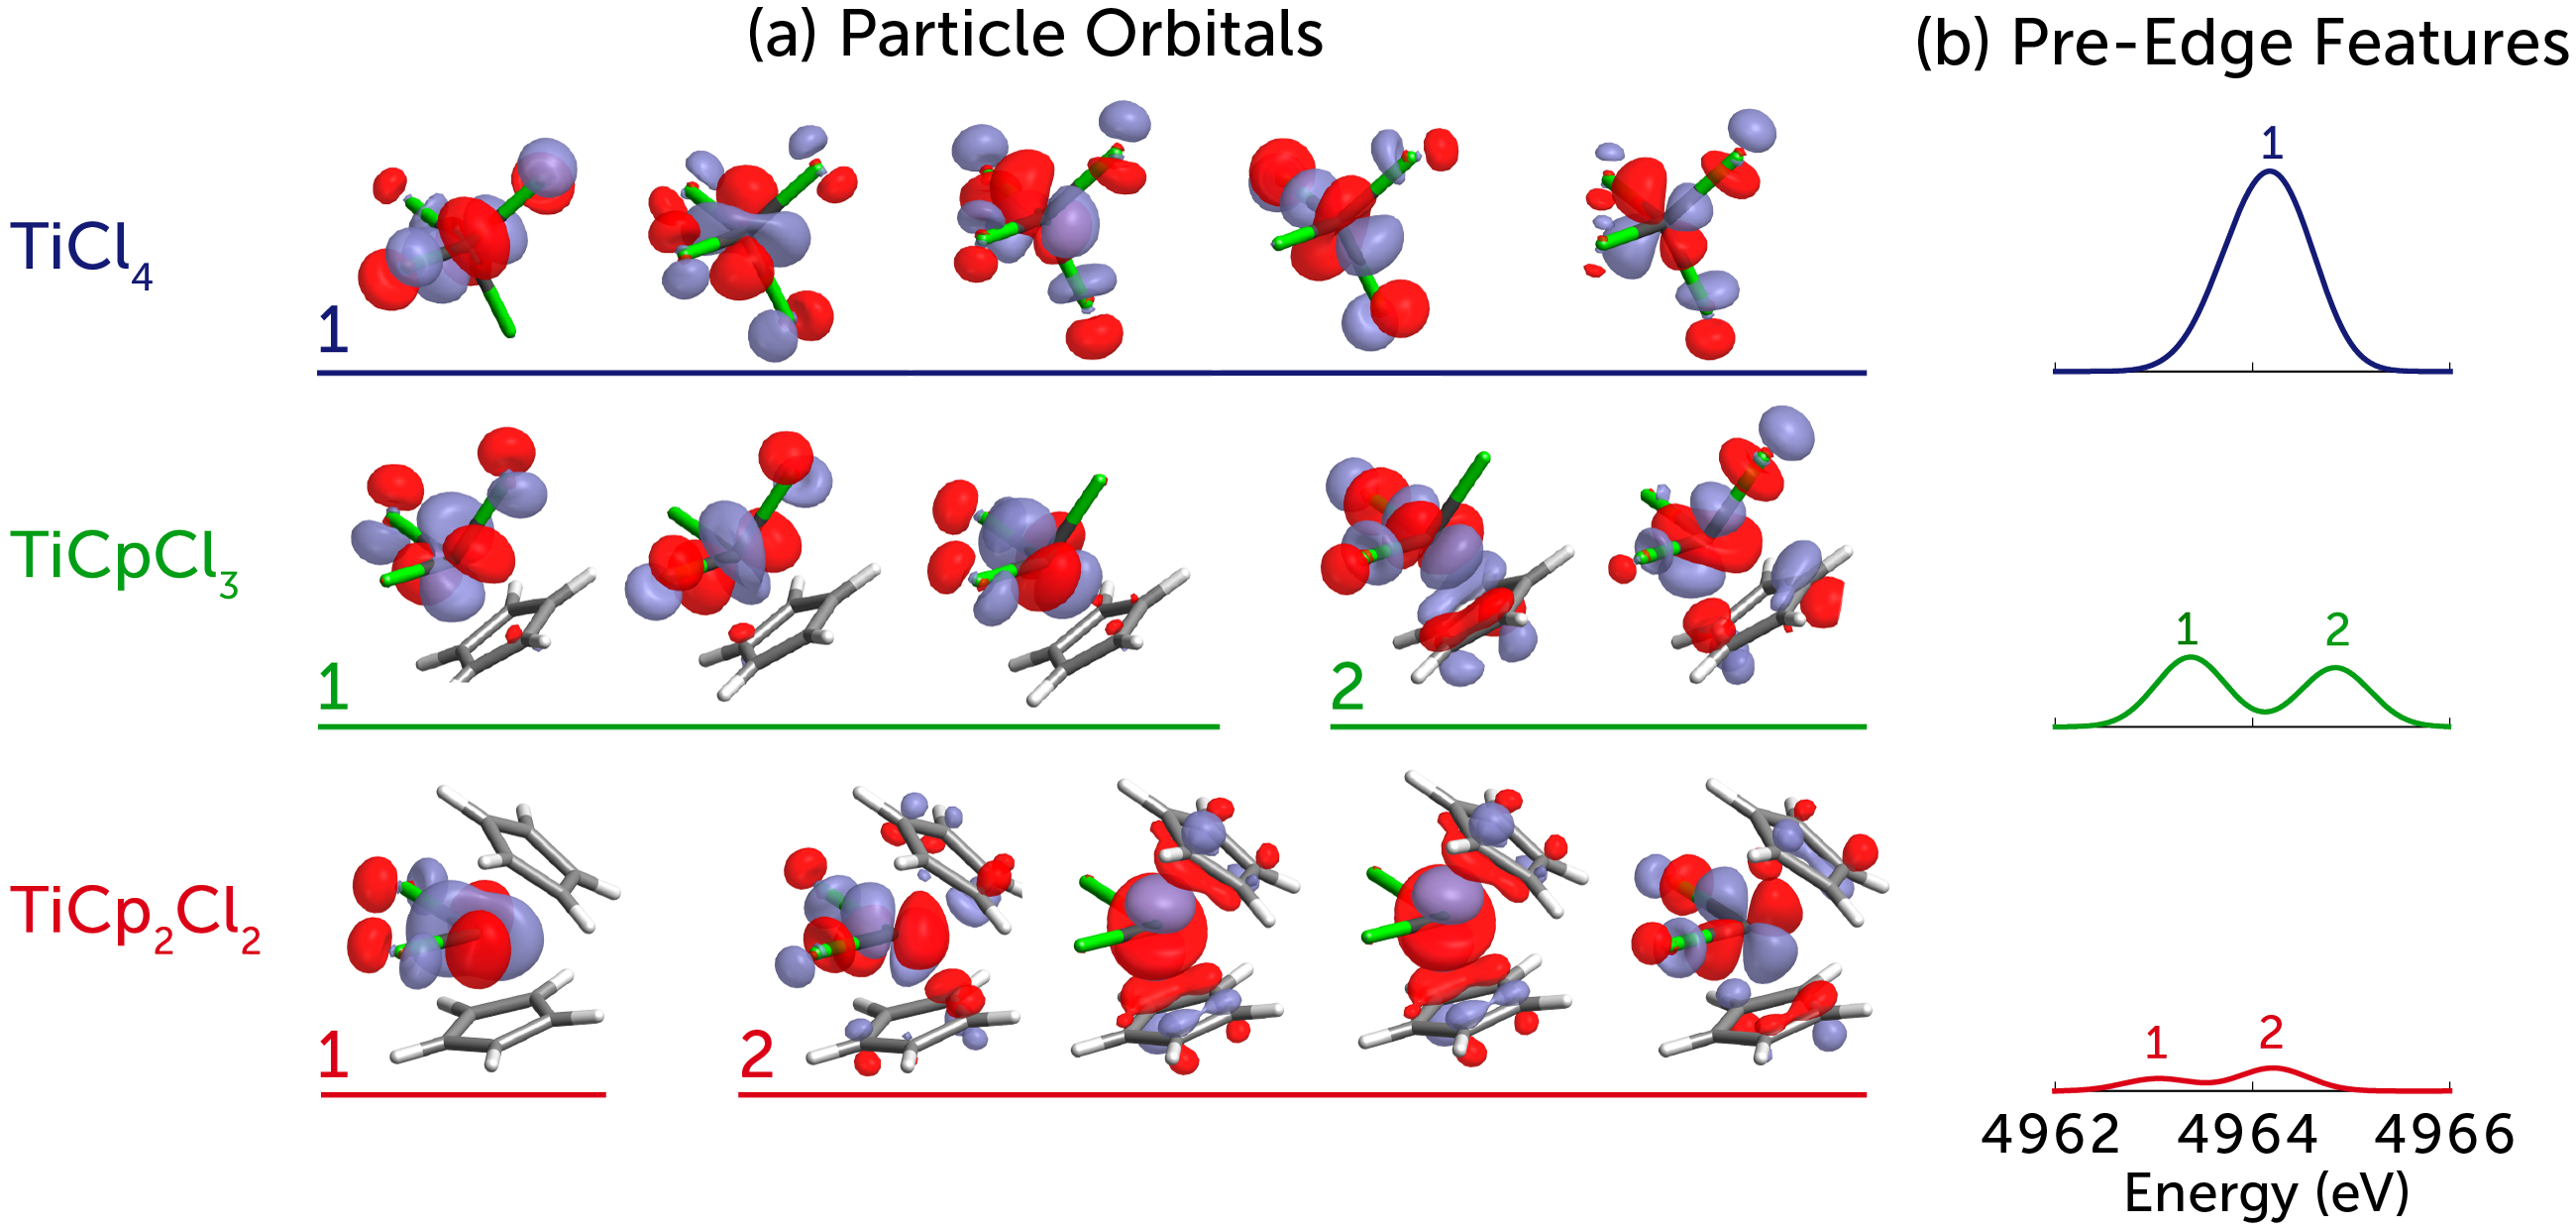
\includegraphics[width=6in]{figure_5.png}
	\caption{(a) Particle orbitals for the core excited states that contribute to the pre-edge features of TiCl$_4$, TiCpCl$_3$, and TiCp$_2$Cl$_2$ and (b) corresponding spectral features.}
	\label{fig:Ti-MOs}
\end{figure*}

To elucidate the nature of the Ti pre-edge features we generated natural atomic orbitals (NAOs),\cite{NBOs} for ground and excited states using the \textsc{janpa}\cite{nikolaienko_janpa:_2014} software interfaced with \textsc{psi4}\cite{PSI4}.
In Table \ref{table:4p_character} we compare the change in orbital shell occupation for each state that contributes to the pre-edge features of the NEXAS spectrum of TiCl$_4$, TiCpCl$_3$, and TiCp$_2$Cl$_2$.
Our analysis reveals that the pre-edge excitations consist mostly of transitions from Ti s to Ti d orbitals and are accompanied by a small increase in population of the Ti p orbitals, and (on average) a decrease in the population of the Cl p shell.

\begin{table*}[t!]
\footnotesize
	\caption{Change in the natural orbital population numbers of the Ti p, Ti d, Cl p shells computed for the Ti pre-edge excitations of TiCl$_4$, TiCpCl$_3$, TiCp$_2$Cl$_2$.}
	\begin{tabular}{lrrrrrrrrr}
		\toprule
		 &  \multicolumn{3}{c}{$\Delta$Ti$_\text{p}$}  & \multicolumn{3}{c}{$\Delta$Cl$_\text{p}$} &  \multicolumn{3}{c}{$\Delta$Ti$_\text{d}$}  \\ \cmidrule(lr){2-4} \cmidrule(lr){5-7} \cmidrule(lr){8-10}
		State & {\text{TiCl$_4$}}  & {\text{TiCpCl$_3$}} & {\text{TiCp$_2$Cl$_2$}}& {\text{TiCl$_4$}}  & {\text{TiCpCl$_3$}} & {\text{TiCp$_2$Cl$_2$}}& {\text{TiCl$_4$}}  & {\text{TiCpCl$_3$}} & {\text{TiCp$_2$Cl$_2$}} \\ \cmidrule(lr){2-4} \cmidrule(lr){5-7} \cmidrule(lr){8-10}
1	&	0.0107	&	0.0066	&	0.0097	&	-0.2184	&	-0.0597	&	0.0051	&	1.1348	&	1.1614	&	1.2586	\\
2	&	0.0126	&	0.0076	&	0.0069	&	-0.3080	&	-0.0513	&	-0.0253	&	1.2111	&	1.1339	&	1.1613	\\
3	&	0.0063	&	0.0088	&	0.0048	&	-0.1790	&	-0.0437	&	-0.0920	&	1.1272	&	1.1256	&	1.0685	\\
4	&	0.0107	&	0.0055	&	0.0050	&	-0.1448	&	-0.0702	&	-0.1038	&	1.0623	&	1.0368	&	1.0633	\\
5	&	0.0064	&	0.0061	&	0.0094	&	-0.0920	&	-0.0829	&	-0.0806	&	1.0403	&	1.0291	&	1.0853	\\
\bottomrule
	\end{tabular}
	\label{table:4p_character}
\end{table*}

DeBeer et al.\cite{TiCl4} have argued that since the Ti 1s to Ti 3d transition is electric dipole forbidden, the pre-edge states must gain intensity through mixing with metal $\text{4p}$ and ligand $\text{3p}$ orbitals.
We have tried to investigate this issue by conducting a Mulliken analysis of the OCDFT transition dipole moment.
In OCDFT, the transition dipole moment for the excitation $\Psi^{(0)} \rightarrow \Psi^{(n)}$ is approximated by the matrix element:
\begin{equation}
\boldsymbol\mu_{0n} = \bra[1]{\Phi^{(n)}}\hat{\mathbf{r}} \ket[1]{\Phi^{(0)}} = \sum_{\mu\nu} D^{0n}_{\mu\nu} \bra{\chi_\mu} \hat{\mathbf{r}} \ket{\chi_\nu}
\end{equation}
where $D^{0n}_{\mu\nu}$ is a transition density matrix and $\bra{\chi_\mu} \hat{\mathbf{r}} \ket{\chi_\nu}$ is the dipole integral in the atomic orbital basis ($\{\chi_\nu\}$).
To analyze each transition we decompose the transition dipole moment into partial atomic contributions.
The contribution to the transition dipole moment arising from the angular moment shell $l_\mathrm{A}$ of a donor atom A to the shell $l_\mathrm{B}$ on the acceptor atom B is expressed as the restricted sum:
\begin{equation}
\label{eq:contribution}
\boldsymbol\mu_{0n} (\mathrm{A}_{l_\mathrm{A}} \rightarrow \mathrm{B}_{l_\mathrm{B}}) = \sum_{\mu \in \mathrm{A}_{l_\mathrm{A}}}\sum_{\nu \in \mathrm{B}_{l_\mathrm{B}}} D^{0n}_{\mu\nu} \bra{\chi_\mu} \mathbf{r} \ket{\chi_\nu}
\end{equation}

Table~\ref{table:ti_analysis_dipole} reports the dominant partial atomic contributions to the transition dipole moment for the pre-edge transitions of TiCpCl$_3$.
For each state we report the three largest contributions to the transition dipole moment, summed over all atoms of the same type.
This analysis reveals that for all pre-edge transitions,the dominant contribution to the transition dipole moment is due to the Ti 4p orbitals.
For example, the transition dipole moment of state 1 can be written as a dominant contribution from Ti s $\rightarrow$ Ti p transitions of magnitude $|\boldsymbol\mu|$ = 41.8$\times 10^{-5}$  au, plus two smaller contributions from ligand-ligand and Ti s $\rightarrow$ Cl p transitions with absolute transition dipole moments of 6.6$\times 10^{-5}$ and 6.4$\times 10^{-5}$ au, respectively.
Other contributions arising from all other combinations of atomic orbitals contribute with a partial transition dipole moment equal to 7.3$\times 10^{-5}$ au.
Note that in many instances the three components of the partial dipole moment have different phases and approximately cancel out.
We observe this pattern also for other pre-edge transitions of TiCpCl$_3$ reported in table~\ref{table:ti_analysis_dipole} and for all transitions of TiCl$_4$ and TiCp$_2$Cl$_2$ (see the supplementary material for a full table of all significant atomic contributions to the pre-edge transitions of the three organotitanium complexes).
In order to assess the stability of this analysis with respect to the size of the basis set, we computed the N$_{1\text{s}}$ $\rightarrow \pi^*$ transition in HCN with six different basis sets: the cc-pV$X$Z series and the corresponding fully uncontracted basis sets, un-cc-pV$X$Z (with $X$ = D, T, Q). As expected, there is variation in the results, however, in all six cases, the most intense atomic contribution was classified as N$_{ \rm s}$ $\rightarrow$ N$_{\rm p}$.

Overall, our OCDFT analysis allows us to quantify the contribution of each atom and orbital shell to the NEXAS peak intensity.We found that peak intensity is acquired mainly from Ti 1s $\rightarrow$ Ti 4p excitations, a result that is in agreement with that proposed by DeBeer et al.\cite{TiCl4}
Interestingly, Ti 1s $\rightarrow$ Cl 3p excitations produce smaller contributions to the total peak intensity, despite the fact that on average the pre-edge transitions are accompanied by a larger change in the occupation of Cl p orbitals than Ti 4p orbital.
This is likely to result from smaller overlap of Ti 1s and Cl p orbitals, which implies a smaller transition dipole moment integral.

\begin{table*}[t!]
	\centering
	\caption{Partial atomic contributions to the transition dipole moment (in atomic units) computed for the pre-edge features of TiCpCl$_3$.}
	\begin{tabular}{lcccc}
		\toprule
		Contribution                  &     $\mu_x$ &     $\mu_y$ &     $\mu_z$ & $|\boldsymbol\mu|$ \\ \midrule
\multicolumn{5}{c}{{\bf{State 1}}}   \\
Ti$_{\rm s}$ $\rightarrow$ Ti$_{\rm p}$ & $-$0.000395 & $-$0.000079 & $-$0.000113 & 0.000418 \\
Cl$_{\rm p}$ $\rightarrow$ Cl$_{\rm p}$ & +0.000062 & +0.000012 & +0.000018 & 0.000066 \\
Ti$_{\rm s}$ $\rightarrow$ Cl$_{\rm p}$ & $-$0.000006 & +0.000003 & $-$0.000064 & 0.000064 \\
Other       & $-$0.000007 & +0.000002 & +0.000073 & 0.000073 \\
\multicolumn{5}{c}{{\bf{State 2}}}   \\
Ti$_{\rm s}$ $\rightarrow$ Ti$_{\rm p}$ & +0.000119 & $-$0.000321 & $-$0.000228 & 0.000411 \\
Ti$_{\rm s}$ $\rightarrow$ Cl$_{\rm p}$ & +0.000013 & $-$0.000000 & $-$0.000143 & 0.000144 \\
Ti$_{\rm s}$ $\rightarrow$ C$_{\rm p}$ & $-$0.000005 & $-$0.000019 & +0.000109 & 0.000111 \\
Other       & $-$0.000027 & +0.000061 & +0.000076 & 0.000101 \\
\multicolumn{5}{c}{{\bf{State 3}}}   \\
Ti$_{\rm s}$ $\rightarrow$ Ti$_{\rm p}$ & $-$0.000038 & $-$0.000289 & +0.000250 & 0.000384 \\
Ti$_{\rm s}$ $\rightarrow$ Cl$_{\rm p}$ & $-$0.000014 & $-$0.000020 & +0.000171 & 0.000173 \\
Ti$_{\rm s}$ $\rightarrow$ C$_{\rm p}$ & +0.000009 & $-$0.000000 & $-$0.000126 & 0.000126 \\
Other       & +0.000016 & +0.000057 & $-$0.000098 & 0.000114 \\
\multicolumn{5}{c}{{\bf{State 4}}}   \\
Ti$_{\rm s}$ $\rightarrow$ Ti$_{\rm p}$ & $-$0.000324 & $-$0.000299 & +0.000003 & 0.000441 \\
Cl$_{\rm p}$ $\rightarrow$ Cl$_{\rm p}$ & +0.000135 & +0.000128 & +0.000005 & 0.000186 \\
C$_{\rm p}$ $\rightarrow$ C$_{\rm p}$ & $-$0.000065 & $-$0.000061 & $-$0.000007 & 0.000089 \\
Other       & $-$0.000021 & $-$0.000015 & +0.000001 & 0.000026 \\
\multicolumn{5}{c}{{\bf{State 5}}}   \\
Ti$_{\rm s}$ $\rightarrow$ Ti$_{\rm p}$ & +0.000304 & $-$0.000313 & +0.000004 & 0.000436 \\
Cl$_{\rm p}$ $\rightarrow$ Cl$_{\rm p}$ & $-$0.000128 & +0.000134 & +0.000003 & 0.000185 \\
C$_{\rm p}$ $\rightarrow$ C$_{\rm p}$ & +0.000060 & $-$0.000062 & +0.000002 & 0.000086 \\
Other       & +0.000021 & $-$0.000024 & $-$0.000007 & 0.000033 \\
		 \bottomrule
	\end{tabular}
	\label{table:ti_analysis_dipole}
\end{table*}

\section{Discussion and Conclusions}

In this study we have combined orthogonality constrained DFT (OCDFT) with the spin-free exact two-component relativistic (X2C) Hamiltonian, and used this as a tool to analyze scalar relativistic effects in the context of core electron excitations.  When relativistic effects are not significant, OCDFT consistently reproduces experimental core-valence excitation energies within 1 eV.
The influence of scalar relativistic effects can already be seen in the failure of nonrelativistic OCDFT at computing core excitation energies of transitions involving the 1s orbital of second-row elements. 
For example, the magnitude of relativistic effects for the Si $\text{1s}$ $\rightarrow$ $\sigma^*$ excitation in SiH$_4$ is estimated to be 4.3 eV, but for the Cl $\text{1s}$ $\rightarrow$ $\sigma^*$ excitation in HCl this figure increases to 10.1 eV. 
We demonstrated that by combining OCDFT with a scalar relativistic Hamiltonian and the B3LYP functional, core excitation energies for second row elements can be computed with an average error of 2.3 eV (from a test set of 10 transitions), a substantial improvement over the 10.3 eV average error observed with the nonrelativistic OCDFT.

Using a class of well studied organotitanium compounds (TiCp$_{n}$Cl$_{4-n}$, n = 2--4), we have demonstrated the utility of the X2C-OCDFT method as a tool to compute accurate transition metal K-edge spectra.
The inclusion of scalar relativistic effects is mandatory to obtain near-quantitative agreement with experimental excitation energies.
For example, for TiCpCl$_3$ we find that a non-relativistic OCDFT treatment predicts excitation energies with an error of about 35 eV.
Once augmented with X2C, the OCDFT error is reduced to 4.8 eV, which is a marked improvement results from relativistic TDDFT (18 eV)\cite{TiCl4-Zeigler}. 
We find that X2C-OCDFT consistently underestimates the pre-edge features of Ti 1s transitions by ca. 5 eV, which is commensurate with our analysis of second row 1$\text{s}$ excitations (MAE = 2.3 eV, max error = 3.6 eV).
In other words, the relative error of X2C-OCDFT Ti K-edge excitation energies is of the order of 0.1\%.
A large portion of the remaining error is most likely due to the use of an approximate functional for the excited state employed in the theory (adiabatic approximation), but also the increased importance of non-scalar relativistic effects (spin-orbit coupling, finite nuclei effects, etc.) that are not captured by spin-free scalar relativistic Hamiltonians.

To gain insight into the nature of the Ti K-edge excitations, we characterize the change in natural atomic orbital population and examine partial atomic contributions to the transition dipole moment of all states that contribute to the pre-edge features.
The character of the pre-edge transitions of the three organotitanium compounds as predicted by OCDFT is consistent with previous analyses,\cite{TiCl4,TiCl4-Zeigler}
however, in this study we developed an approach to quantify partial atomic contributions to the transition dipole moments.
This tool enables us to attribute most of the pre-edge peak intensity to excitations involving Ti 4p orbitals.  Ligand orbitals are found to give small contributions to the peak intensity.

What contributes to the improved performance of OCDFT with respect to TDDFT for core excitation energies?
Our evidence suggests that like other $\Delta$SCF based approaches,\cite{STEX,Besley-EOM-MOM,Thomas,Voorhis,Ziegler-1,Besley-Gill} OCDFT derives an advantage from the fact that it can properly describe charge-transfer excitations.\cite{Casida-TDDFT-CT-problem,Zeigler-TDDFT-CT-problem}
To illustrate this point, we computed the C and O K-edge spectrum of CO using various functionals and interpreted our data using a toy model of that captures the charge-transfer character of core excitations.
Our analysis suggests that a large source of the error in TDDFT arises from double counting the change in Coulomb energy that results from unpairing a core electron.
In the case of OCDFT, the effects of double counting the Coulomb repulsion is smaller, and the energy expression involves only local self-interaction terms.
We also note a stronger dependence of the TDDFT spectrum on the amount of Hartree--Fock exchange included in the functional.
Although shifted TDDFT will be comparable to OCDFT results, they are not identical, and there exists significant merit in performing OCDFT calculations since it yields more consistent predictions.
%In our analysis we have focused on the charge-transfer-like nature of core excited states.

One future application of this work is to extend OCDFT to the computation of L-edge spectra. The L-edge is composed of excitations from core 2p orbitals and simulation of the full spectrum will require proper treatment of spin-orbit coupling effects due to mixing of excitations from degenerate 2p orbitals. We would also like to explore the idea of using this orthogonality constrained excited state framework to build wave function based methods with the same advantages seen in OCDFT. This would allow us to create systematically improvable schemes that do not rely on approximate exchange-correlation functionals.


\section*{Acknowledgments}
This work was supported by start-up funds provided by Emory University. We would like to thank Dr. Lan Cheng for providing data to benchmark our implementation of X2C We would also like to acknowledge Dr. Tymofii Y. Nikolaienko for providing help with the JANPA software package. W.D.D. is supported by the National Science Foundation Graduate Research Fellowship under Grant No. 0000048655. Any opinion, findings, and conclusions or recommendations expressed in this material are those of the authors and do not necessarily reflect the views of the National Science Foundation.

{\footnotesize
\bibliography{biblio}
\bibliographystyle{achemso}
}
\end{document}
\documentclass{article}
    % General document formatting
    \usepackage[margin=0.7in]{geometry}
    \usepackage[parfill]{parskip}
    \usepackage[utf8]{inputenc}
    \usepackage{graphicx}
    \usepackage[sort&compress,numbers,super]{natbib}
    \usepackage{booktabs}
    
    % Related to math
    \usepackage{amsmath,amssymb,amsfonts,amsthm}
\begin{document}
\chapter{Localized Intrinsic Valence Virtual Orbitals as a Tool for the Automatic Classification of Core Excited States}
\epigraph{\textit{``We must be clear that when it comes to atoms, language can be used only as in poetry. The poet, too, is not nearly so concerned with describing facts as with creating images and establishing mental connections''}}{Niels H. D. Bohr}
\begin{chapabstract}
Accurate assignments of the unoccupied molecular orbitals involved in electronic excited states are crucial to the interpretation of experimental spectra. Here we present an automated approach to the assignment of excited states by introducing a unique orbital basis known as localized intrinsic valence virtual orbitals (LIVVOs), which are a special case of the previously reported valence virtual orbitals. The LIVVOs are used to quantify the local contributions to particle orbitals from orthogonality-constrained density functional theory, providing an assignment with atomic-level/angular momentum shell specificity. This localized set also allows us to define the total valence character of an excited state. We highlight the utility of our approach by studying the local orbital changes in core-excited states at the sulfur K-edge of ethanethiol and benzenethiol as well as hydrogen bonding in the water dimer.
\end{chapabstract}
% Introduction
\section{Introduction}
Any interpretation of electronic spectroscopy depends upon assigning spectral features of the experimental spectrum to discrete electronic transitions calculated using excited state quantum chemistry methods. This requires characterization of the molecular orbitals involved in the discrete transition. Transitions are usually assigned by visual inspection of the contributing virtual molecular orbitals (MOs). Often, when these MOs do not have well defined character, orbital labels are used instead (e.g. LUMO, LUMO + 1, etc.). These approaches are somewhat unsatisfactory. The assignment of orbital character based on MO plots is potentially ambiguous. Furthermore, characterizing a transition using orbital labels is problematic because virtual orbitals are not uniquely defined and they strongly depend on the basis set and level of theory employed. 

A unique branch of electronic spectroscopy involving the excitation of core electrons using X-ray photons called near-edge X-ray absorption fine structure (NEXAFS) spectroscopy has garnered particular interest due to advancements in high-resolution tunable synchrotron light sources. NEXAFS spectroscopy has become an indispensable experimental tool for probing local electronic and geometrical information in a wide variety of molecular systems. \cite{westre_multiplet_1997,loble_covalency_2015-1,idrees_oxidation_2014,nelson_introduction_2012-1} The significant features of the NEXAFS spectrum arise from core orbital to unoccupied valence orbital transitions. \cite{stohr_nexafs_1992-1} The atomic nature of the core orbitals involved in these transitions (1s, 2s, 2p, etc.) makes NEXAFS a spectroscopic technique for elucidating local electronic structure information. Quantum chemistry calculations serve as a vital tool for gleaning meaningful electronic structure information from NEXAFS spectra including the nature of unoccupied orbitals, orbital mixing effects, and covalent character.\cite{stohr_nexafs_1992-1,loble_covalency_2015-1,nelson_introduction_2012,milne_recent_2014-1,cabaret_first-principles_2010-1}
A myriad of theoretical methods have been developed for the computation of core-excited states, ranging from rigorous methods focused on high accuracy \cite{coriani_coupled-cluster_2012,nooijen_description_1995,besley_equation_2012,peng_energy-specific_2015-1,dutta_intermediate_2014-1,brabec_communication:_2012,sen_study_2013-1,schirmer_beyond_1982-2,salpeter_relativistic_1951-1,barth_theoretical_1980,butscher_all-electron_1977-1,roemelt_excited_2013,asmuruf_calculation_2008,grimme_density_1996,lopata_linear-response_2012-2,fernando_x-ray_2015}
to computationally efficient methods focused on applications to larger systems.\cite{rehr_theoretical_2000,natoli_multiple_2012-1,joly_x-ray_2001,lowdin_statistical_1972,stener_time_2003-1,besley_time-dependent_2010-2,lestrange_calibration_2015,kuramoto_theoretical_2005,ohtsuka_inner-shell_2006,kolczewski_detailed_2001-1} The primary motivation underpinning these theoretical developments has been to obtain more accurate excitation energies and/or oscillator strengths. In contrast, the character of the wave function is analyzed in a more cursory fashion.

A recent work by the group of Dreuw\cite{wenzel_physical_2016,plasser_new_2014,plasser_new_2014-1} has taken a significant step toward a more rigorous description of core-excited states.
Using the one-particle transition density matrix and the one-particle difference density matrix, these authors were able to quantify the effects of relaxation, estimate multireference character, and provide information on the exciton size. These methods are a significant step toward a robust characterization of excited-states.
Myhre, Coriani, and Koch\cite{myhre_near-edge_2016} also recently used visualization of the one-particle difference density matrix in order to track the localization of core-excited states, relying on analysis of the excitation amplitudes of coupled cluster response calculations to assign the character of core-valence transitions. Although a fair amount of attention has been put forth to add a breadth of different descriptors for excited states, little attention has been put toward trying to improve upon the method of assigning orbital character.

Canonical molecular orbitals often complicate the assignment process because valence virtual MOs are mixed with polarization and diffuse functions included in the basis set.
A common approach to obtain more chemically meaningful valence orbitals is to project the virtual space onto a set of atomic valence orbitals. This approach hinges on the assumption that valence atomic orbitals are the dominant contributors to the valence molecular orbitals. This assumption was justified in the 1980s by Rudenberg and coworkers by obtaining overlaps close to unity between free-atom AOs and their projection onto the molecular orbitals of MCSCF wave functions. \cite{ruedenberg_are_1982}
Perhaps, the most popular method to analyze wave functions in terms of atomic valence contributions is Weinhold's natural atomic/bond orbital (NAO/NBO) analysis.\cite{foster_natural_1980,reed_natural_1985} This method partitions the full density matrix into atomic sub-blocks that are diagonalized in order to produce atom-localized hybrid valence orbitals.
AO projection based methods have been presented throughout the literature including polarized atomic orbitals, \cite{lee_extracting_2000-1,subotnik_fast_2005} enveloping localized orbitals,\cite{auer_dynamically_2006-1} intrinsic minimal atomic basis orbitals,\cite{laikov_intrinsic_2011-1} molecule-adapted atomic orbitals, \cite{szczepanik_minimal_2013-1} and intrinsic atomic orbitals. \cite{knizia_intrinsic_2013}
The approach presented in this work is based on the valence virtual orbitals (VVOs) scheme. \cite{lu_molecule_2004}
VVOs are built by bringing virtual valence MOs into maximum coincidence with a minimal atomic basis set via a unitary transformation.
The VVOs have been used with success to identify the valence LUMO in a variety of molecular systems,\cite{schmidt_valence_2015} to characterize bond breaking/formation along dissociation pathways,\cite{west_comprehensive_2015-1} and as a set of starting orbitals for multi-configurational SCF calculations.\cite{west_comprehensive_2013} VVOs can be easily localized and provide an accurate representation of the localized valence antibonding orbitals in a molecule. 

In this work we report a new method for automated classification of virtual orbitals in electronic excited states by quantifying the local contributions using a localized set of VVOs.
To generate the VVOs an accurate atomic minimal basis set (AAMBS) that spans the atomic valence space is required. We propose to represent the AAMBS using a minimal basis set of quasiatomic orbitals.\cite{lu_molecule_2004}
These are generated using projection operators according to Knizia's intrinsic atomic orbitals (IAOs) procedure\cite{knizia_intrinsic_2013} and localized using the Pipek--Mezey localization scheme. \cite{pipek_fast_1989}
The combination of VVOs projected onto a localized intrinsic orbital basis is abbreviated as LIVVOs.
To compute excitation energies we employ our recently proposed orthogonality-constrained DFT (OCDFT) approach\cite{evangelista_orthogonality_2013} to compute a manifold of states.\cite{derricotte_simulation_2015}
OCDFT is a variational time-independent DFT method built upon a generalized Kohn-Sham scheme.
In OCDFT excited state energies are approximated by a Kohn--Sham procedure augmented with orthogonality constraints between ground and excited state wave functions.

This new classification method is applied to the core-excited states involved in NEXAFS spectroscopy. We utilize the quantification of local contributions to analyze substituent effects in  thiols (ethanethiol, benzenethiol) and intermolecular interactions in the water dimer. The thiols were chosen as an example of molecules where the relevant excited states have significant contributions from more than one valence antibonding MO. Previous studies have not fully characterized the antibonding character of orbitals involved in core-valence excitations.\cite{behyan_chemical_2014,behyan_sulfur_2013,behyan_sulfur_2011}  We show that we are able to provide insight into the nature of these excited states using LIVVOs. Hydrogen bonding interactions in water have received plenty of attention within the X-ray absorption community.\cite{wernet_structure_2004,cavalleri_interpretation_2002,smith_probing_2006,prendergast_x-ray_2006-2,iannuzzi_x-ray_2008,leetmaa_theoretical_2010,kuhne_nature_2014}
Studies have shown that NEXAFS spectral changes upon the formation of a hydrogen bond is a result of localization of excited states along either the free OH bond or the hydrogen bond.\cite{smith_probing_2006,prendergast_x-ray_2006-2,kuhne_nature_2014,tse_x-ray_2008,smith_energetics_2004,smith_response_2005,chen_x-ray_2010,clark_structure_2010,vinson_theoretical_2012}
However, the degree of localization has not been quantified.  In this work we show that LIVVOs help quantify the localization of core excited states of the water dimer and that this metric is correlated some some spectral features.

%
% Theory 
%
\section{Theory}

\begin{figure*}[h!]
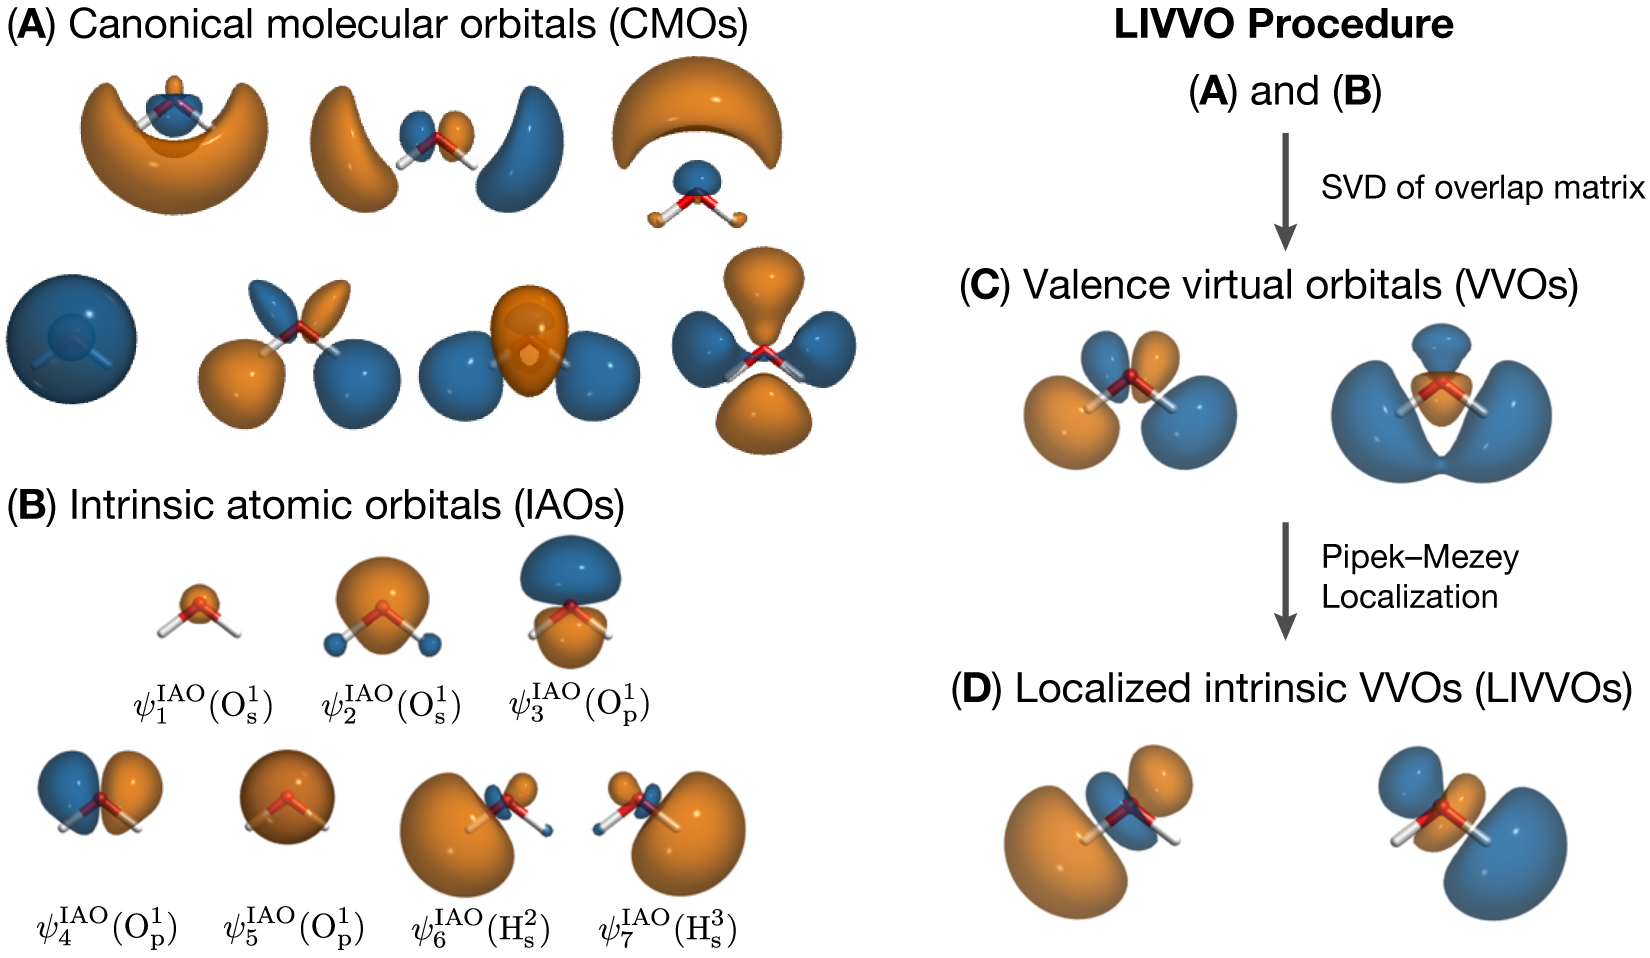
\includegraphics[width=5.5in]{figure_1_vvo_localization.png}
\caption{Illustration of the procedure used to construct localized intrinsic valence virtual orbitals (LIVVOs). (A) Canonical molecular orbitals (CMOs) of water computed at the B3LYP/aug-cc-pVTZ level of theory. (B) Intrinsic atomic orbitals obtained from the CMOs of water and corresponding assignment to a given atom and angular momentum shell.
(C) Delocalized valence virtual orbitals (VVOs) obtained by singular value decomposition of the overlap matrix [eq~\eqref{eq:overlap}]. 
(D) Localized intrinsic valence virtual orbitals (LIVVOs) for water after Pipek-Mezey localization of the VVOs.}
\label{fig:vvo_localization}
\end{figure*}

In this section we discuss three aspects of our approach to analyze core excitations.
First, we consider the construction of the localized intrinsic valence virtual orbitals (LIVVOs) from canonical molecular orbitals (CMOs) and intrinsic atomic orbitals (IAOs).
Next, we discuss how to automate the determination of the atomic character of the  IAOs and the LIVVOs.
Finally, we discuss the procedure used to analyze the particle orbital in OCDFT computations of core-excited states.

\subsection{Construction of Localized Intrinsic Valence Virtual Orbitals}
Here we summarize the construction of VVOs and discuss how to obtain the LIVVOs.
The procedure outlined here is illustrated in Figure~\ref{fig:vvo_localization} for the case of water.
The construction of VVOs begins by first identifying the virtual subset of the canonical molecular orbitals ($\{ \phi_a\}$) from a ground state SCF calculation.
The virtual CMOs are expanded in an atom-centered basis $\{\chi_{\mu}\}$ and are expressed in terms of MO coefficients $C_{\mu a}$
\begin{align}
|\phi_a\rangle = \sum_{\mu}^{N_\mathrm{AO}} |\chi_{\mu} \rangle C_{\mu a}, \quad a = 1,\ldots,N_\mathrm{vir}
\end{align}
where $N_\mathrm{AO}$ and $N_\mathrm{vir}$ are the number of atomic and virtual orbitals, respectively.
As shown in Figure~\ref{fig:vvo_localization}A, the virtual CMOs may have contributions from diffuse functions and their valence character is difficult to interpret.

To identify the valence character of the CMOs, we perform a VVO analysis\cite{Lu:2004cw,Lu:2004gq,schmidt_valence_2015} using the intrinsic atomic orbitals (IAOs) of Knizia\cite{knizia_intrinsic_2013} as the underlying accurate atomic minimal basis set.
IAOs are a set of orthonormal polarized atomic orbitals that can exactly express the occupied molecular orbitals of the ground state Kohn-Sham (KS) determinant $| \Phi \rangle$.
IAOs are expressed in terms of the atomic orbital basis as
\begin{align}
|\psi_{\rho}^\mathrm{IAO}\rangle = \sum_{\mu}^{N_\mathrm{AO}} |\chi_{\mu} \rangle \tilde{C}_{\mu \rho}, \quad \rho = 1, \ldots, N_\mathrm{IAO}
\end{align}
where $\tilde{C}_{\mu \rho}$ is the IAO coefficient matrix and $N_\mathrm{IAO}$ is the number of IAO orbitals.
As shown in Figure~\ref{fig:vvo_localization}B, in the case of water there are 7 IAOs that correspond to the oxygen atom 1s, 2s, and 2p shells and a single 1s orbital for each hydrogen atom.

Next, the overlap matrix ($\mathbf{S}$) of the canonical virtual orbitals with the IAO  functions $\psi_{\rho}^\mathrm{IAO}$ is evaluated:
\begin{align} \label{eq:overlap}
(\mathbf{S})_{a\rho} = \langle \phi_a | \psi_{\rho}^\mathrm{IAO} \rangle
\end{align}
and as suggested in Ref. \citenum{schmidt_valence_2015} a singular value decomposition (SVD) is performed on $\mathbf{S}$:
\begin{align}
\mathbf{S} = \mathbf{U} \boldsymbol{
\sigma} \mathbf{V}^{\dagger}
\end{align}
to yield orthogonal transformation matrices ${\bf U}$ and ${\bf V}$.
These matrices are rotations of the virtual space and the IAO space, respectively, that bring the two sets of orbitals into maximum coincidence.
The number of VVOs ($N_{\rm VVO}$) is given by the number of IAOs minus the number of occupied molecular ($N_{\rm occ}$) orbitals: $N_{\rm VVO} = N_{\rm IAO} - N_{\rm occ}$.
Assuming that the singular value decomposition orders the singular values ($\sigma_v$) in descending order, then the VVOs are obtained by transforming the canonical virtual orbitals with the first $N_{\rm VVO}$ columns of the matrix $\mathbf{U}$:
\begin{equation}
\label{eq:orbital_rotation}
| \psi^{\rm VVO}_v \rangle = \sum_a^{N_\mathrm{vir}} | \phi_a \rangle U_{av}, \quad v = 1, \ldots, N_{\rm VVO}.
\end{equation}

The VVOs for water shown in Figure~\ref{fig:vvo_localization}C, have valence character and correspond to the plus and minus combination of localized $\sigma^*_\text{O--H}$ orbitals.
Following Pipek--Mezey localization,\cite{pipek_fast_1989} we arrive at a set of localized VVOs that span the antibonding interactions of the molecular environment. We refer to this localized set as localized intrinsic valence virtual orbitals (LIVVOs). In the case of water, when the VVOs are localized we obtain the $\sigma^*_\text{O--H}$ orbitals drawn in Figure~\ref{fig:vvo_localization}D.

\subsection{Determination of the character of the IAOs and LIVVOs}
The goal of our analysis is to express excited states using the LIVVO basis. In addition, we are also interested in determining the dominant atomic character of each excited state.
To this end, we have automated the analysis of the atomic character of the LIVVOs.
Our approach starts with the assignment of the atomic character of each IAO via a Mulliken population analysis.\cite{mulliken_electronic_1955,mulliken_electronic_1955-1}
For each IAO, $\psi_{\rho}^\mathrm{IAO}$, we compute the population matrix:
\begin{equation}
P_{\mu\nu}(\rho) = \tilde{C}_{\mu \rho} S_{\mu\nu} \tilde{C}_{\nu \rho}, \quad \rho = 1, \ldots, N_\mathrm{IAO}
\end{equation}
Gross populations on atom $A$ and angular momentum shell $l$ [GP$_{A_l}(\rho)$] are obtained as partial sums of the population matrix:
\begin{equation}
\mathrm{GP}_{A_{l}}(\rho)  = \sum_{\mu \in A_{l}} \sum_{\nu}^{N_\mathrm{AO}} P_{\mu\nu}(\rho) 
\end{equation}
where the sum over $\mu$ is restricted to all functions centered on atom $A$ with angular momentum quantum number  ${l}$.

Values of $\mathrm{GP}_{A_{l}}(\rho)$ for the water example are reported in Table \ref{tab:iao_atomic}.
The assignment of IAOs using the gross population is straightforward since there is always a dominant contribution from a single atom/shell.
For example, in the case of IAO $\psi^{\rm IAO}_6$, the largest contribution to $\mathrm{GP}_{A_{l}}(\rho)$ is from the H$_\mathrm{s}^2$ shell (1.18), followed by smaller contributions from the O$_\mathrm{s}^1$, O$_\mathrm{s}^1$, and H$_\mathrm{s}^3$ shells (with absolute value less or equal to 0.08).
Therefore, we define the character of $\psi_{\rho}^\mathrm{IAO}$ as the pair atom/shell ($A$,${l}$) for which $\mathrm{GP}_{A_{l}}(\rho)$ is maximum:
\begin{equation}
 \mathrm{character}(\psi_{\rho}^\mathrm{IAO}) = \arg\max_{(A,{l})} \mathrm{GP}_{A_{l}}(\rho) \label{eq:ioa_character}
\end{equation}
In the case of water, when eq~\eqref{eq:ioa_character} is applied to the IAOs we obtain the assignment reported in Figure~\ref{fig:vvo_localization}B.

\begin{table}[b]
\renewcommand{\arraystretch}{1.2}
\footnotesize
\centering
\caption{Atom-centered gross orbital populations [GP$_{A_l}(\rho)$] for the seven IAOs of water. Calculations were performed at the B3LYP/jun-cc-pVTZ level of theory.}
\begin{tabular}{r@{\hskip6pt}r@{\hskip6pt}r@{\hskip6pt}r@{\hskip6pt}r@{\hskip6pt}r@{\hskip6pt}r@{\hskip6pt}r}
\toprule
$A_{l}$ & $\psi^{\rm IAO}_1$ & $\psi^{\rm IAO}_2$ & $\psi^{\rm IAO}_3$ & $\psi^{\rm IAO}_4$& $\psi^{\rm IAO}_5$& $\psi^{\rm IAO}_6$& $\psi^{\rm IAO}_7$ \\[3pt]
\midrule
O$_\mathrm{s}^1$ & 1.00 & 1.16 & 0.00 & 0.00 & 0.00 & $-$0.08 & $-$0.08 \\
O$_\mathrm{p}^1$ & 0.00 & 0.00 & 1.04 & 1.11 & 1.00 & $-$0.07 & $-$0.07 \\
H$^2_\mathrm{s}$ &0.00 & $-$0.08 & $-$0.02 & $-$0.05 & 0.00 & 1.18&  $-$0.03\\
H$^3_\mathrm{s}$ & 0.00 & $-$0.08 & $-$0.02 & $-$0.05 & 0.00 & $-$0.03 & 1.18\\
\bottomrule
\end{tabular}
\label{tab:iao_atomic}
\end{table}
\setlength{\tabcolsep}{0.1em}

Once the atomic character of each IAO is determined, we characterize the atomic contributions to each LIVVO.
For each LIVVO, $\psi_l^{\rm LIVVO}$, we evaluate the overlap with all the IAOs ($\psi^{\rm IAO}_{\rho}$):
\begin{equation}
\label{eq:livvo_iao_overlap}
S'_{l \rho} = | \langle \psi_l^{\rm LIVVO} | \psi^{\rm IAO}_{\rho} \rangle |^2
\end{equation}
The initial step in classifying the LIVVOs is to determine their overall orbital character ($\sigma$,$\pi$,\ldots).
A LIVVO is classified as $\sigma^*$ if the largest elements of $S'_{l \rho}$ include contributions from IAOs with $s$ and $p$ character.
Similarly, a LIVVO is assigned $\pi^*$ character if the largest elements of $S'_{l \rho}$ arise exclusively from $p$-type IAOs.
The atoms involved in the LIVVO are identified by the character of the  largest elements of $S'_{l \rho}$.
For this purpose, we only include those IAOs whose overlap with a given LIVVO is greater than a threshold, which in the following examples is set to 0.1.

To illustrate this analysis we consider the case of acrolein ($\rm C_3H_4O$).
The following LIVVOs are characterized respectively as $\sigma^*_\text{C$^2$--C$^3$}$ and $\pi^*_\text{C$^2$--C$^3$}$:
\begin{equation*}
\begin{split}
\vcenter{\hbox{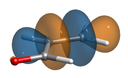
\includegraphics[width = 2.5cm]{img_1a}}} =& 
\, 0.20 \, \psi^{\rm IAO}(\rm C^2_s) + 0.24 \, \psi^{\rm IAO}(\rm C^2_p) \\
& + 0.20 \, \psi^{\rm IAO}(\rm C^3_s)  + 0.25 \, \psi^{\rm IAO}(\rm C^3_p) \\
\\
\vcenter{\hbox{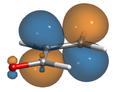
\includegraphics[width = 2.25cm]{img_1b}}} =& \,
 0.47 \, \psi^{\rm IAO}(\rm C^2_p)  + 0.51 \,  \psi^{\rm IAO}(\rm C^3_p)  
\end{split}
\end{equation*}
Note that the in the case of the $\sigma^*_\text{C$^2$--C$^3$}$ LIVVO there are contributions from both s and p orbitals, while 98\% of the $\pi^*_\text{C$^2$--C$^3$}$ LIVVO is comprised of p orbitals.
The construction and analysis of the LIVVOs is fully automated and is performed only once after a ground state KS computation.

\subsection{Analysis of OCDFT Particle Orbitals Using LIVVOs}
The procedure used to generate the LIVVOs relies only the information contained in the reference ground state determinant and is therefore applicable to any method.
The focus of this work is to apply the LIVVO to OCDFT computations of K-edge spectra.
First, we briefly summarize the features of OCDFT.
In OCDFT,\cite{evangelista_orthogonality_2013} a generalized Kohn--Sham picture is assumed, where to the $n$-th electronic state corresponds an auxiliary system of noninteracting electrons with wave function $\Phi^{(n)}$ and density $\rho^{(n)}$. The wave function for the auxiliary system is a single Slater determinant, $\ket{\Phi^{(n)}} = \ket[1]{\phi_1^{(n)}\phi_2^{(n)} \cdots\phi_N^{(n)}}$, where the set of orbitals $\{\phi_i^{(n)}\}$ are different for each electronic state. To avoid variational collapse, OCDFT enforces orthogonality conditions between all determinants:
\begin{equation}
\label{eq:OCcondition}
\langle \Phi^{(m)} | \Phi^{(n)} \rangle = \delta_{mn} \;\;\;  \forall m,n
\end{equation}

In this work we employ our constrained multiple hole/particle (CMHP) algorithm\cite{ayers_time-independent_2012} for the solution of multiple orthogonally constrained excited states.
The CMHP scheme fully accounts for relaxation of all orbitals, but rather than solving for the exact minimum orthogonality conditions, it imposes  sufficient orbital orthogonality conditions. Namely, we assume that the hole orbitals in core-excited states are localized and are orthogonal.
It follows then that one-electron excited states can be characterized by fully relaxed hole [$\phi_{\rm h}^{(n)}$] and particle [$\phi_{\rm p}^{(n)}$] orbitals, which span the occupied and virtual spaces of the ground state wave function, respectively.

For every excited state, we analyze the character of the particle orbital $\phi_{\rm p}^{(n)}$ by evaluating its overlap with each LIVVO ($\psi^{\rm LIVVO}_l$):
\begin{equation}
\label{eq:part_livvo_overlap}
\Omega_{\mathrm{p}l}^{(n)} = | \langle \phi^{(n)}_\mathrm{p} | \psi^{\rm LIVVO}_l \rangle |^2.
\end{equation}
The individual overlaps $\Omega_{\mathrm{p}l}^{(n)}$ are used to assign the character of the particle orbital to the $l$-th LIVVO.
In addition, we also define the total valence character $t^{\mathrm{val},(n)}_\mathrm{p} $ for any given particle orbital as the sum its overlap with all LIVVOs:
\begin{equation}
t^{\mathrm{val},(n)}_\mathrm{p} = \sum_{l}^{N_\mathrm{LIVVO}} \Omega_{\mathrm{p}l}^{(n)}.
\label{eq:total_valence_character}
\end{equation}
Since the LIVVOs give an accurate representation of valence orbitals in the molecule, it is possible to quantify the most important local contributions to the particle orbital. While this offers a very robust description for localized valence particle orbitals, it is important to note that the particle orbital describing the excited state can also be fairly diffuse with respect to the molecular environment. Such an orbital will obviously have relatively low overlap with the LIVVOs described here. This can be a desirable feature of our method as it allows for immediate identification of spectral contributions that arise from more diffuse orbitals. 
However, any further classification of the diffuse nature or Rydberg character of virtual orbitals is outside the scope of the current study.

\section{Computational Details}
OCDFT is currently implemented as a plugin for the PSI4 \cite{turney_psi4:_2012-1} \textit{ab initio} quantum chemistry package. All core excitation energies and oscillator strengths are obtained using the B3LYP \cite{lee_development_1988-1,becke_new_1993-3,vosko_accurate_1980-2,stephens_ab_1994-2} functional and a triple zeta correlation-consistent basis set jun-cc-pVTZ,\cite{woon_gaussian_1993-1,dunning_gaussian_1989-1} which is obtained by deleting diffuse functions from the highest subshell of every atom in the aug-cc-pVTZ basis set.\cite{papajak_perspectives_2011} The two-electron integrals are factorized using the density-fitting approximation\cite{dunlap_firstrow_1979,schrader_use_1962,baerends_self-consistent_1973,dunlap_robust_2000-1,dunlap_applicability_1977-1} with the jun-cc-pVTZ-JKFIT auxillary fitting basis.\cite{weigend_accurate_2006-2,weigend_hartreefock_2008}
Basis set dependence of the LIVVO analysis is investigated using the cc-pVXZ and aug-cc-pVXZ (X=D,T,Q) family of basis sets.\cite{kendall_electron_1992,dunning_gaussian_1989-1}
Intrinsic atomic orbitals were obtained using Robert Parrish's implementation in PSI4.\cite{Parrish:2014de}
The geometries for ethanethiol, benzenethiol, water monomer, and water dimer were all optimized at the B3LYP/aug-cc-pVTZ level of theory.

Peak intensities for each transition from the ground state to excited state ($n$) are based on the oscillator strength ($f_{\rm osc}$):
\begin{align}
f_{\rm osc} = \frac{2}{3}|\boldsymbol{\mu}_{n0}|^2\omega_n
\end{align}
where $\omega_n$ is the excitation energy calculated in OCDFT and $\boldsymbol{\mu}_{n0}$ is the transition dipole moment vector. OCDFT does not provide a direct route toward computation of the transition dipole moments, however, these can be approximated using the noninteracting Kohn--Sham determinants:
\begin{equation}
\boldsymbol{\mu}_{n0} = \langle \Phi^{(n)}|\mathbf{r}| \Phi^{(0)} \rangle
\label{eq:dipole}
\end{equation}
where $\Phi^{(n)}$ is the KS determinant for the $n$-th excited state and $\mathbf{r}$ is the position vector.
Spectroscopic broadening effects are simulated by representing each transition using a Gaussian lineshape with a FWHM of 0.4 eV.

\section{Results}
\subsection{Analysis of substituent effects in the spectra of thiols}

\begin{table*}[!t]
\renewcommand{\arraystretch}{1.2}
\centering
\footnotesize
\caption{Transition energies, oscillator strengths ($f_{\rm osc}$), and LIVVO assignments for all states calculated in the NEXAFS spectrum of ethanethiol and benzenethiol. Experimental energies and assignments are taken from Ref. \citenum{behyan_sulfur_2011}.}
\begin{tabular}{@{\extracolsep{6pt}}cccrcr@{}}
\toprule
& \multicolumn{3}{c}{OCDFT} & \multicolumn{2}{c}{Experiment} \\
\cline{2-4} \cline{5-6}
State & Energy (eV) & $f_{\rm osc}$ & LIVVO Assignment & Energy (eV)  & Assignment\\
\midrule
\multicolumn{6}{c}{\bf{Ethanethiol}} \\
1 & 2472.9 & 0.0022 & 58\% $\sigma^*_{\rm S^3-H^9}$ & 2472.2 & $\sigma^*_{\rm S-H}$ \\
& & & 22\% $\sigma^*_{\rm S^3-C^2}$\vspace{0.1cm} & & Weak $\sigma^*_{\rm S-C}$\\
2 & 2473.9 & 0.0011 & 57\% $\sigma^*_{\rm S^3-C^2}$ & 2473.1 & $\sigma^*_{\rm S-C}$ \\
& & & 18\% $\sigma^*_{\rm S^3-H^9}$\vspace{0.1cm} & &\\
3 & 2475.6 & 0.0004 & 9\% $\sigma^*_{\rm C^2-H^8}$ & 2474.9 & Poorly Defined \\
& & & 7\% $\sigma^*_{\rm C^2-H^7}$\vspace{0.1cm} & &\\
4 & 2476.2 & 0.0007 & 8\% $\sigma^*_{\rm S^3-C^2}$ & & \\
& & & 5\% $\sigma^*_{\rm C^2-H^8}$\vspace{0.1cm} & &\\
5 & 2476.1 & 0.0005 & 6\% $\sigma^*_{\rm C^1-H^6}$ & & \\
& & & 3\% $\sigma^*_{\rm C^2-H^7}$\vspace{0.1cm} & &\\
\multicolumn{6}{c}{\bf{Benzenethiol}} \\
1 & 2472.9 & 0.0023 & 61\% $\sigma^*_{\rm S^7-H^8}$ & 2472.4 & $\sigma^*_{\rm S-H}$\\
& & &  22\% $\sigma^*_{\rm S^7-C^3}$ & & Weak $\sigma^*_{\rm S-C}$ \vspace{0.1cm}\\
2 & 2474.2 & 0.0011 & 53\% $\sigma^*_{\rm S^7-C^3}$ & 2473.5  & Weak $\pi^*_{C=C}$ \\
& & & 16\% $\sigma^*_{\rm S^7-H^8}$\vspace{0.1cm} & &\\
3 & 2474.9 & 0.0001 & 68\% $\pi^*_{\rm C^{2,3,4}}$ & 2475.3 & $\sigma^*_{S-C}$ \\
& & & 15\% $\pi^*_{\rm C^{4,5,6}}$\vspace{0.1cm} & &\\
4 & 2475.3 & 0.0000 & 48\% $\pi^*_{\rm C^{1,2,6}}$ & &\\
& & & 34\% $\pi^*_{\rm C^{4,5,6}}$ & & \vspace{0.1cm}\\
5 & 2476.0& 0.0006 & 7\% $\sigma^*_{\rm S^7-H^8}$ & &\vspace{0.1cm}\\
\bottomrule
\end{tabular}
\label{tab:thiols}
\end{table*}





\begin{figure}[!b]
\centering
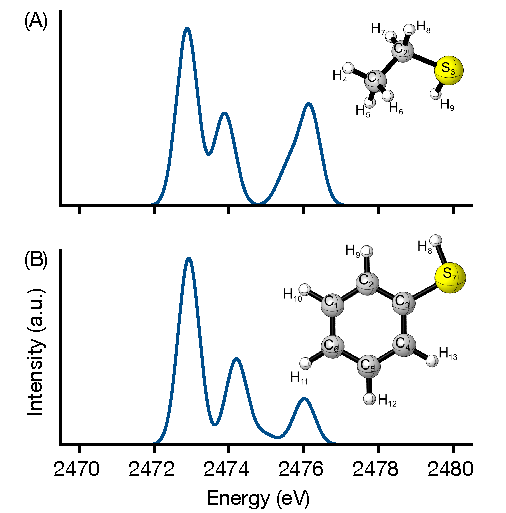
\includegraphics{figure_2_thiols_spectra.pdf}
\caption{Sulfur 1s near-edge x-ray absorption spectra of thiols calculated with OCDFT at the B3LYP/jun-cc-pVTZ level of theory. Spectra of (A) ethanethiol and (B) benzenethiol. Shown in the inset of each spectrum is the optimized structure for each molecule. Structures were plotted using CYLview software.\cite{legault_cylview_2009}}
\label{fig:thiols}
\end{figure}

\begin{figure*}[h]
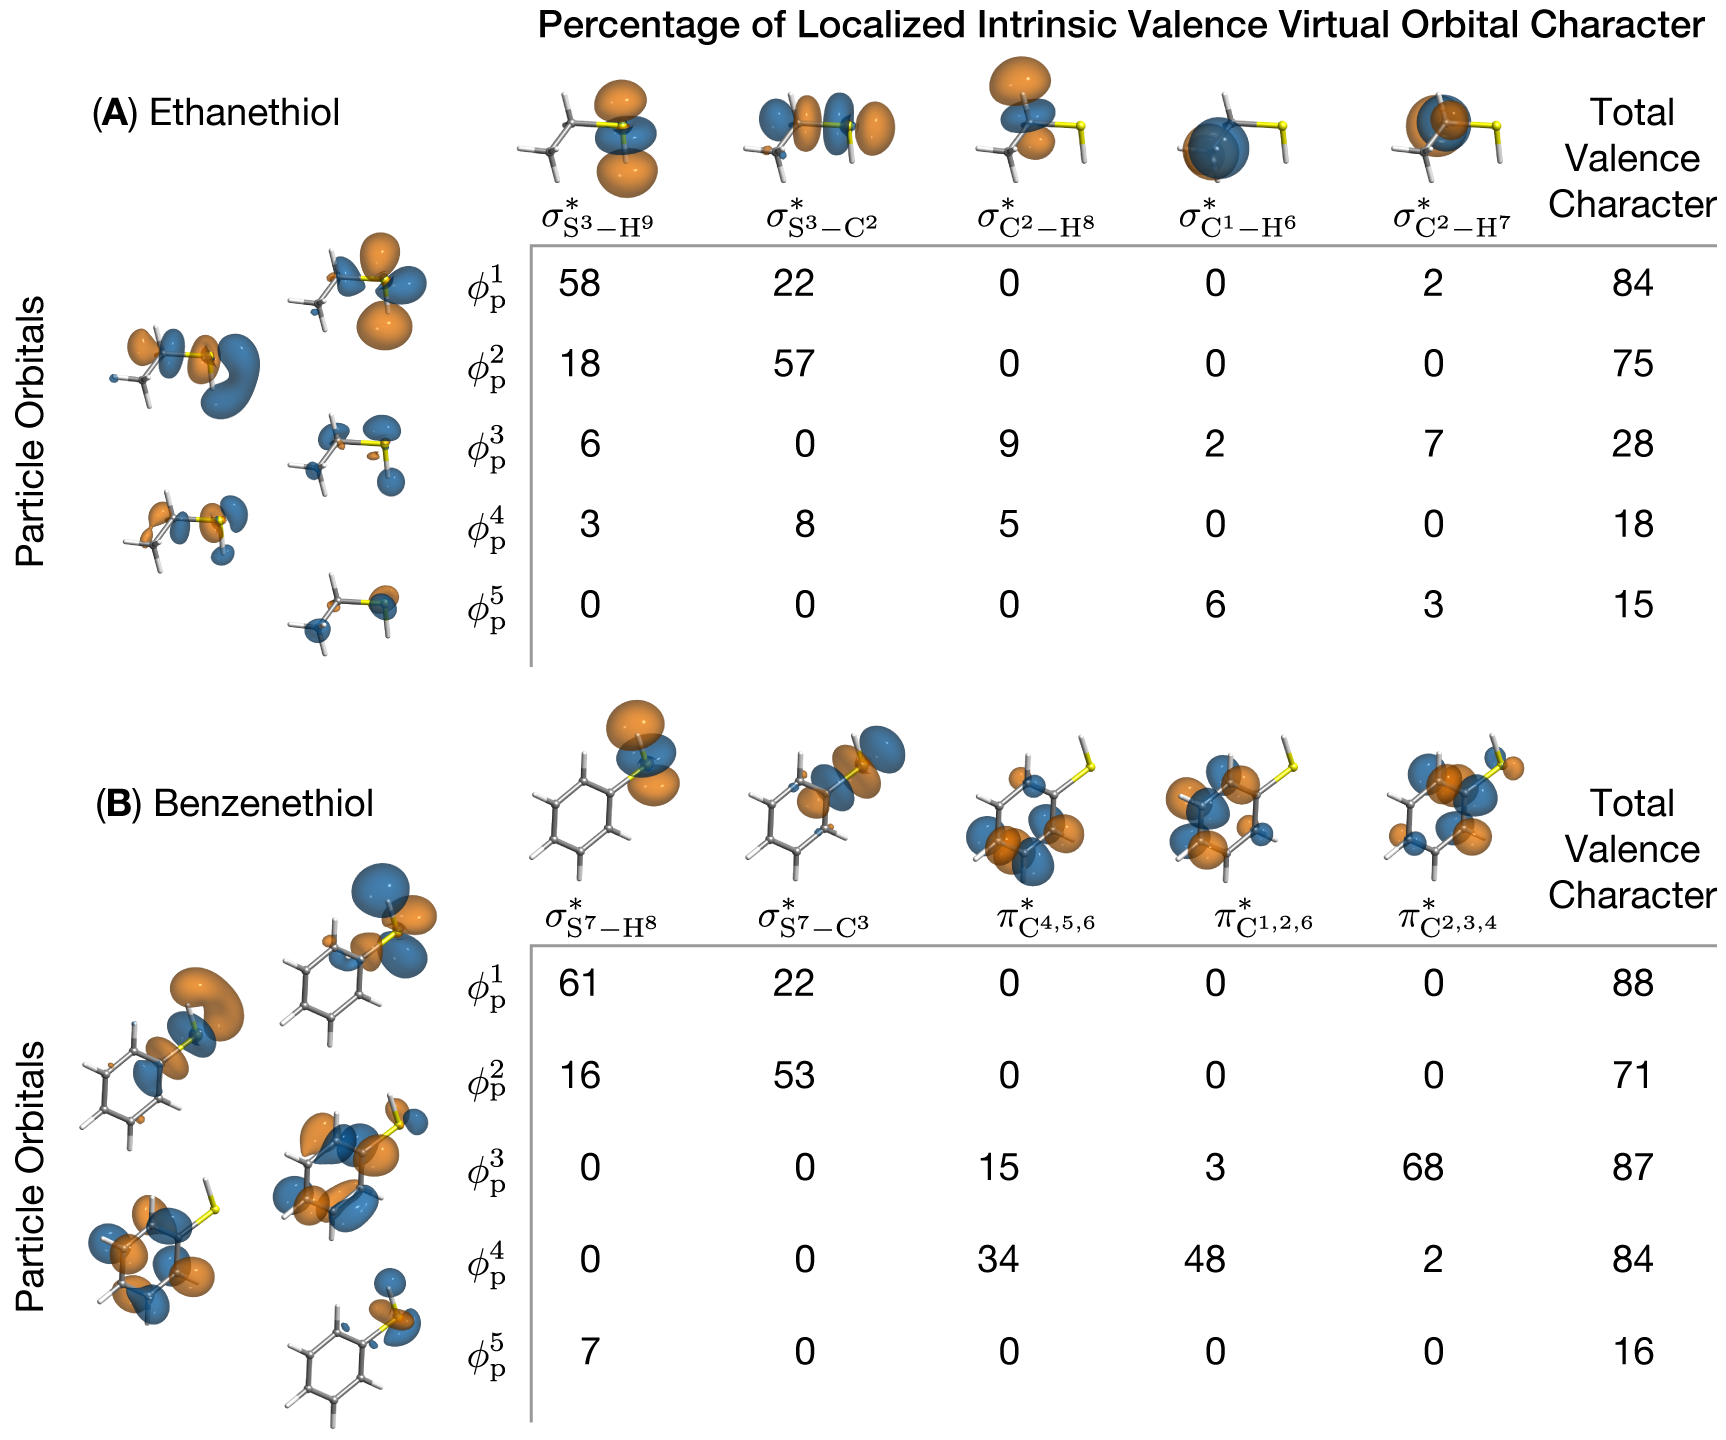
\includegraphics[width=5.75in]{figure_3_livvo_analysis_thiols.png}
\caption{Particle orbitals, valence virtual orbitals, and total valence character for each of the five core transitions in the NEXAFS spectrum of (A) ethanethiol (C$_2$H$_5$SH) and (B) benzenethiol (C$_6$H$_5$SH). Percentages shown represent the overlap of each particle orbital with the LIVVOs. Particle orbitals are numbered according to the calculated transitions reported in Table \ref{tab:thiols} while atom numberings correspond to those shown in Figure~\ref{fig:thiols}.}
\label{fig:thiols_cont}
\end{figure*}

Our first application of the LIVVO analysis for the classification of NEXAFS spectral features focuses on the effect of substituents on peak position and intensity.
In this section we compare the sulfur K-edge of ethanethiol (C$_2$H$_5$SH) and benzenethiol (C$_6$H$_5$SH).
The OCDFT NEXAFS spectra for these two compounds are shown in Figure~\ref{fig:thiols}.
Table \ref{tab:thiols} reports a comparison of experimental and theoretical excitation energies, OCDFT oscillator strengths, the LIVVO assignments, and total valence character for each state. 

The gas-phase experimental excitation energies shown in Table \ref{tab:thiols} for ethanethiol represents the three peaks of the spectrum at 2472.17, 2473.11, and 2474.87 eV. Our calculated OCDFT spectrum is also characterized by three peaks with transition energies that are in good agreement with the experimental spectrum. The first two are a result of strong single transitions at  2472.9 and 2473.9 eV. The final peak is a combination of three weak transitions that occur at 2475.6, 2476.2, and 2476.1 eV. 

The gas phase experimental spectrum of benzenethiol is characterized by three peaks at 2472.4, 2473.5, and 2475.3 eV. The theoretical spectrum has strong single transitions at 2472.9 eV and 2474.2 eV. The last peak is composed of weaker transitions at 2474.9, 2475.3, and 2476.0 eV.
In total, this gives us errors that are on average less than 1.0 eV across these two molecules. This agreement with the experimental spectrum is consistent with that seen in previous studies with OCDFT\cite{derricotte_simulation_2015,verma_predicting_2016} and are obtained without application of shifts to match experimental values.

By analyzing the overlap of the particle orbitals with all orbitals in the LIVVO basis, it is possible to quantify the degree of localization along each bond and discern the origin of some features of the ethanethiol and benzenethiol spectra.
The lowest energy transition in the NEXAFS spectrum of ethanethiol and benzenethiol occurs at  at 2472.9 eV, and was attributed mostly to a S 1s $\rightarrow$ $\sigma^*_\text{S--H}$ transition with a ``weak'' contribution from a S 1$s$ $\rightarrow$ $\sigma^*_\text{S--C}$ transition.\cite{behyan_sulfur_2013}
The LIVVO assignments, displayed in Figure~\ref{fig:thiols_cont}, show that in both cases the first state (corresponding to the particle orbital $\phi_\mathrm{p}^1$) can be assigned to $\sigma^*_\text{S--H}$ (50\%) and $\sigma^*_\text{S--C}$ (22\%) character. Going from ethanethiol to benzenethiol there is a slight increase in the degree of localization along the thiol bond. This is evidenced by the $\sigma^*_\text{S--H}$ character of the first excited state increasing from 58\% in ethanethiol, to 61\% in benzenethiol.

The second peak in the NEXAFS spectra of the thiols occurs at 2473.9 eV for  ethanethiol and at 2474.2 eV for benzenethiol. Again in this case, simple inspection of the particle orbitals ($\phi_\mathrm{p}^2$) shows orbital character along both the S--H and S--C bonds. The LIVVO assignments show that over 50\% of the character of the particle orbital can be assigned to the $\sigma^*_{\rm S-C}$ orbital in each molecule, while less than 19\% can be assigned to the $\sigma^*_{\rm S-H}$ orbital. Comparing our results with a previous study\cite{behyan_sulfur_2013} that employed the Hartree--Fock static exchange (HF-STEX) method, \cite{otero_nitrogen_2006,cooney_chemical_2004,urquhart_core_1997,urquhart_probing_1998,urquhart_near-edge_1999,kosugi_rydberg_1995} our assignments agrees well for the case of ethanethiol.
However, the OCDFT assignment is at odds with their assignment for benzenethiol where they attributed this peak feature to core transitions to $\pi^*$ orbitals associated with the phenol ring. The discrepency in this assignment likely stems from the differences in the energy ordering of the virtual orbitals between HF and DFT.

The third peak in the spectrum for both thiols is a combination of three low-intensity transitions. Of these, the most intense transition is predicted by OCDFT to be at 2476.2 eV for ethanethiol and 2476.0 eV for benzenethiol and corresponds to the particle orbital $\phi_\mathrm{p}^4$.
Considering the total valence characters shown in Figure~\ref{fig:thiols_cont} and the oscillator strengths shown in Table \ref{tab:thiols}, we see a clear trend relating the valence character and the oscillator strength of the transition.
In the case of ethanethiol, the low valence character of the transitions (28\% or lower) suggests that the smaller oscillator strength of the third peak is due to the diffuse mixed Rydberg character of particle orbitals $\phi_\mathrm{p}^3$, $\phi_\mathrm{p}^4$, and $\phi_\mathrm{p}^5$.

In the case of benzenethiol, the valence character of states $\phi_\mathrm{p}^3$ and $\phi_\mathrm{p}^4$ is high (87\% and 84\%, respectively) but these orbitals are mostly localized on the phenyl ring and give small contributions to the transition dipole moment.
State $\phi_\mathrm{p}^3$ is a mixture of $\pi^*_{\mathrm{C}^{2,3,4}}$ and $\pi^*_{\mathrm{C}^{4,5,6}}$ at 68\% and 15\% respectively, while state $\phi_\mathrm{p}^4$ is a mixture of $\pi^*_{\mathrm{C}^{1,2,6}}$ and $\pi^*_{\mathrm{C}^{4,5,6}}$ at 48\% and 34\% respectively.
This analysis suggests that the small overlap of these states with the sulfur atom is the cause of the small intensity of the corresponding transitions.
State $\phi_\mathrm{p}^5$ of benzenethiol has a much lower total valence character (16\%), however, since it has 7\% overlap with the $\sigma^*_{\rm S-H}$ thiol bond orbital, the corresponding transition still has a modest intensity.
We should note that thanks to the LIVVO analysis we were able to quantify the weak local contributions to the states that contribute to the third peak.
Previous studies\cite{behyan_sulfur_2013} were unable to assess the orbital character of this set of transitions.

\subsection{Signatures of hydrogen bonding in the NEXAFS spectrum of the water dimer}

\begin{table}[!t]
\renewcommand{\arraystretch}{1.2}
\centering
\footnotesize
\caption{Transition energies, oscillator strengths ($f_{\rm osc}$), and LIVVO assignments for all states calculated in the NEXAFS spectrum of the water monomer, dimer-A, and dimer-D.}
\begin{tabular}{@{\extracolsep{6pt}}cccr@{}}
\toprule
State & Energy (eV) & $f_{\rm osc}$ & LIVVO Assignment\\
\midrule
\multicolumn{4}{c}{\bf{Monomer}} \\
1 & 533.7 & 0.00811 & 42\% $\sigma^*_{\rm O_1-H_2}$ \\
 & & & 42\% $\sigma^*_{\rm O_1-H_3}$ \\
 2 & 535.4 & 0.01839 & 38\% $\sigma^*_{\rm O_1-H_2}$ \\
 & & & 38\% $\sigma^*_{\rm O_1-H_3}$ \\
 3 & 537.3 & 0.00786 & Rydberg/Diffuse \\
 4 & 537.8 & 0.00252 & Rydberg/Diffuse \\
 5 & 538.5 & 0.00167 & 6\% $\sigma^*_{\rm O_1-H_2}$ \\
 & & & 6\% $\sigma^*_{\rm O_1-H_3}$ \\
 \multicolumn{4}{c}{\bf{Dimer-A}} \\
 1 & 534.0 & 0.00737 & 41\% $\sigma^*_{\rm O_1-H_2}$ \\
 & & & 41\% $\sigma^*_{\rm O_1-H_3}$ \\
  2 & 535.8 & 0.01862 & 39\% $\sigma^*_{\rm O_1-H_2}$ \\
 & & & 39\% $\sigma^*_{\rm O_1-H_3}$ \\
   3 & 537.7 & 0.00552 & 14\% $\sigma^*_{\rm O_4-H_5}$ \\
 & & & 9\% $\sigma^*_{\rm O_4-H_6}$ \\
   4 & 537.9 & 0.00529 & 4\% $\sigma^*_{\rm O_4-H_6}$ \\
 & & & 3\% $\sigma^*_{\rm O_4-H_5}$ \\
   5 & 539.3 & 0.00282 & 12\% $\sigma^*_{\rm O_4-H_6}$ \\
 & & & 8\% $\sigma^*_{\rm O_4-H_5}$ \\
  \multicolumn{4}{c}{\bf{Dimer-D}} \\
 1 & 533.5 & 0.00605 & 52\% $\sigma^*_{\rm O_4-H_6}$ \\
 & & & 16\% $\sigma^*_{\rm O_4-H_5}$ \\
  2 & 534.9 & 0.00878 & 24\% $\sigma^*_{\rm O_4-H_6}$ \\
 & & & 18\% $\sigma^*_{\rm O_1-H_2}$ \\
   3 & 536.1 & 0.00574 & 3\% $\sigma^*_{\rm O_1-H_2}$ \\
 & & & 3\% $\sigma^*_{\rm O_1-H_3}$ \\
   4 & 536.6 & 0.00284 & 2\% $\sigma^*_{\rm O_4-H_5}$ \\
 & & & 2\% $\sigma^*_{\rm O_1-H_3}$ \\
   5 & 537.3 & 0.00623 & 25\% $\sigma^*_{\rm O_4-H_5}$ \\
 & & & 5\% $\sigma^*_{\rm O_4-H_5}$ \\
\bottomrule
\end{tabular}
\label{tab:water_spec}
\end{table}

Due to the critical role it plays in many processes in nature, hydrogen bonding is one of the most important noncovalent interactions in chemistry.\cite{morokuma_why_1977,kool_hydrogen_2001,fonseca_guerra_hydrogen_2000,stiopkin_hydrogen_2011,pflugrath_sulphate_1985}
The water dimer (H$_2$O)$_2$ is one of the simplest yet most important examples of hydrogen bonding in chemistry and has garnered plenty of attention from both theory and experiment. \cite{feyereisen_hydrogen_1996,kim_comparison_1994,reed_natural_1983,stevens_frozen_1987,szalewicz_theoretical_1988,headrick_spectral_2005,wang_multimode_2008,chng_experimental_2012,shank_accurate_2009,mukhopadhyay_water_2015,gomez_partition-dft_2017,zhang_quantitative_2017} This simple dimer is the basic building block of the structures of liquid water and ice, which have both been studied extensively with NEXAFS spectroscopy to uncover their underlying hydrogen bond coordination.\cite{wilson_x-ray_2001,wilson_characterization_2002,parent_structure_2002} A host of computational methods have been applied to study the effects of hydrogen bonding on the NEXAFS spectrum of water, including transition potential DFT (TPDFT), \cite{prendergast_x-ray_2006-2,iannuzzi_x-ray_2008,leetmaa_theoretical_2010,hetenyi_calculation_2004,cavalleri_half_2005} coupled-cluster singles and doubles (CCSD), \cite{coriani_coupled-cluster_2012,coriani_asymmetric-lanczos-chain-driven_2012,fransson_requirements_2016} and complex polarization propagator DFT (CPP-DFT). \cite{ekstrom_x-ray_2006} Here, we utilize our LIVVO analysis in order to quantify these effects on the NEXAFS spectrum.  


\textit{Water monomer}. 
A host of computational methods have been applied to study the effects of hydrogen bonding on the NEXAFS spectrum of water, including transition potential DFT (TPDFT), \cite{prendergast_x-ray_2006-2,iannuzzi_x-ray_2008,leetmaa_theoretical_2010,hetenyi_calculation_2004,cavalleri_half_2005} coupled-cluster singles and doubles (CCSD), \cite{coriani_coupled-cluster_2012,coriani_asymmetric-lanczos-chain-driven_2012,fransson_requirements_2016} and complex polarization propagator DFT (CPP-DFT). \cite{ekstrom_x-ray_2006}. Here, we utilize our LIVVO analysis in order to quantify these effects on the NEXAFS spectrum.  
Figure~\ref{fig:water_spec}A shows the NEXAFS spectrum for water monomer and the lowest-energy configuration of the water dimer.
To facilitate our analysis, we separate the dimer spectrum into contributions from the hole localized on the oxygen accepting the hydrogen bond (O$_1$, denoted as dimer-A) and a spectrum for the hole localized on the oxygen donating the hydrogen bond (O$_4$, denoted as dimer-D).
These partial contributions are shown in panels B and C of Figure~\ref{fig:water_spec}, respectively.
Table \ref{tab:water_spec} shows all of the calculated excitation energies, oscillator strengths and final LIVVO assignments for each state.

\begin{figure}[t!]
\centering
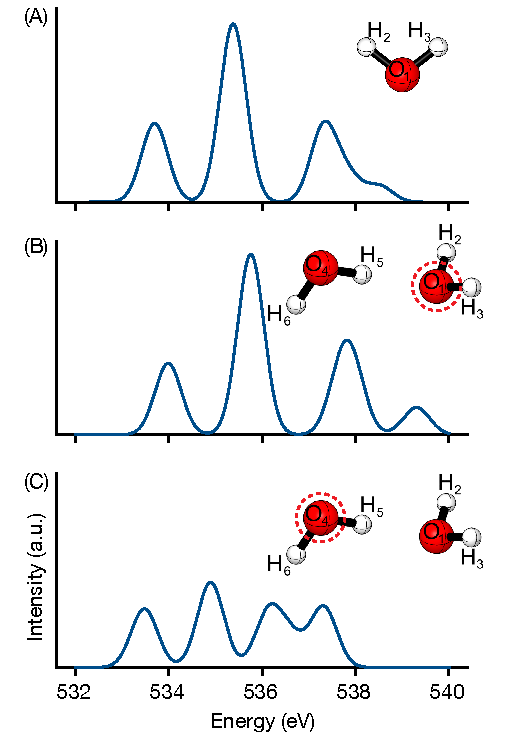
\includegraphics{figure_4_water_spectra.pdf}
\caption{Oxygen 1s Near-edge x-ray absorption spectra of: (A) water monomer, (B) dimer-A, and (C) dimer-D calculated with OCDFT at the B3LYP/jun-cc-pVTZ level of theory. Shown in the inset of each spectrum is the optimized structure for each molecule. For the water dimer, we indicate the core-excited atom with a red cicle. Structures were plotted using the CYLview software.\cite{legault_cylview_2009}}
\label{fig:water_spec}
\end{figure} 

The OCDFT computed NEXAFS spectrum of water monomer at the O K-edge, shown in Figure~\ref{fig:water_spec}, is defined by three characteristic peaks at 533.7, 535.4, and 537.3 eV respectively.
The positions of these peaks are in excellent agreement with the gas-phase experimental peak features which occur at 534.0, 535.9, and 537.0 eV. \cite{schirmer_k-shell_1993}
The first peak at 533.7 eV has a relative intensity of 0.44 and is characterized by the particle orbital $\phi^1_{\rm p}$ shown in Figure~\ref{fig:water_all_livvo}A, while the second peak at 535.4 is the most intense of the spectrum and is characterized by the particle orbital $\phi^2_{\rm p}$.
Two Rydberg transitions at 537.3 and 537.8 eV contribute to the third peak in the spectrum and are accompanied by a higher energy shoulder feature at 538.5 eV.

The water monomer particle orbitals are shown in Figure~\ref{fig:water_all_livvo}A along with the overlap with the LIVVOs and their total valence character. The first two transitions in the water monomer are heavily localized resulting in total valence character of 85\% and 75\%, respectively.
The three higher energy transitions are to more diffuse orbitals, as evidenced by the extremely low total valence percentages (in the range 0--12 \%). Rydberg transitions that contain no overlap with the LIVVO basis due to their high degree of delocalization can not be assigned a well-defined valence character and are labeled ``Rydberg/Diffuse'' in Table \ref{tab:water_spec}. Analyzing the contributions of each LIVVO to the respective particle orbitals reveals that for this case, both the $\sigma^*_\text{O$_1$--H$_2$}$ and $\sigma^*_\text{O$_1$--H$_3$}$ LIVVOs contribute equally to each excited state. This is a characteristic feature of particle orbitals in the spectrum of the water monomer and will be useful in the comparison with the water dimer spectrum. 

\textit{Water dimer, hydrogen bond acceptor}. 
The spectra for localized excitations in the water dimer shown in panels B and C of Figure~\ref{fig:water_spec} allow us to discern features that arise from hydrogen bonding in the accepting and donating water molecules.
Comparing panels A (monomer) and B (dimer-A) of Figure~\ref{fig:water_spec},  the two spectra are very similar with three distinct peaks. The first two core excitations for the dimer-A spectrum occur at 534.0 and 535.8 eV and exhibit a 0.3 and 0.4 eV blueshift, respectively, when compared to the monomer. The oscillator strengths are also similar, with the second transition being the most intense in the spectrum, and the first transition having similar oscillator strength in the dimer-A (0.00737) and monomer (0.00811) spectra.

The similarities between these transitions becomes obvious when comparing  the particle orbitals for the monomer and the dimer (shown in Figure~\ref{fig:water_all_livvo}).
The particle orbitals for the first two transitions in the dimer-A spectrum have no contribution from the donating water molecule and are localized exclusively on the accepting water molecule. In addition, the particle orbitals $\phi_\mathrm{p}^1$ and $\phi_\mathrm{p}^2$ for the dimer-A look nearly identical to those for the water monomer.
These two particle orbitals are localized on the hydrogen atoms of the acceptor water and thus are weakly perturbed by the hydrogen bond. 
In contrast, the three higher energy transitions show some degree of delocalization onto the donating water molecule.

The LIVVOs can be used in an effort to quantify the degree of localization/delocalization in the particle orbitals involved. Water dimer contains four LIVVOs, two that are localized on the accepting water ($\sigma^*_{\rm O_1-H_2}$ and $\sigma^*_{\rm O_1-H_3}$), one that is localized on the free OH bond in the donor water ($\sigma^*_{\rm O_4-H_6}$), and one that represents the hydrogen bonding interaction between the two water molecules ($\sigma^*_{\rm O_4-H_5}$).
While similar in orbital character to the other LIVVOs,  $\sigma^*_{\rm O_4-H_5}$ has contributions from the accepting water molecule which gives us a direct way to track the overlap of an excited state orbital with O-H antibonding interaction from the hydrogen bond.

The values reported in Figure \ref{fig:water_all_livvo}B correspond to the percentage of overlap between each water dimer LIVVO and the  particle orbitals contributing to the dimer-A spectrum. Considering that orbitals $\phi_{\rm p}^1$ and $\phi_{\rm p}^2$ are heavily localized on the accepting water, it is unsurprising that the first two states have equal contributions from the LIVVOs localized on the accepting water ($\sigma^*_{\rm O_1-H_2}$ and $\sigma^*_{\rm O_1-H_3}$). The total valence character of these states (84\% and 77\%) is similar to the total valence character of the first two particle orbitals in the monomer spectrum (85\% and 75\%), implying that the presence of the donor water has a negligible effect on $\phi_{\rm p}^1$ and $\phi_{\rm p}^2$. It is encouraging to see that our LIVVO analysis parallels the uniformity seen in these states with regard to their orbital character, peak position, and peak intensity.

The three particle orbitals corresponding to higher energy transitions in the dimer-A spectrum ($\phi_{\rm p}^3$, $\phi_{\rm p}^4$, $\phi_{\rm p}^5$) have significant overlap with $\sigma^*_{\rm O_4-H_5}$ and $\sigma^*_{\rm O_4-H_6}$. It is in this higher energy region of the spectrum where we see the most significant distinctions between the dimer-A and monomer spectrum. The monomer spectrum shows a shoulder feature at higher energy while in the dimer-A this shoulder feature is now a distinct peak at higher energy. Our analysis based on LIVVOs shows that states 3, 4, and 5 experience a stark increase in total valence character from 0\%, 0\%, and 12\% respectively in the monomer to 23\%, 7\%, and 29\% in the dimer-A. This drastic increase in valence character is caused by interactions with the donor water, in all cases the final LIVVO assignments (shown in Table \ref{tab:water_spec}) can be attributed to the two LIVVOs localized on the donor water. The spectral changes seen in this region of the dimer-A spectrum can be rationalized by the presence of distinct orbital character from the donor water. This result is particularly encouraging, since simple inspection of the particle orbitals give little indication of these contributions from the donor water. In fact, especially in the cases of $\phi_{\rm p}^3$ and $\phi_{\rm p}^4$, these contributions look fairly insignificant. However our analysis reveals that these seemingly harmless contributions account for a majority, if not all of the total valence character for these states.

\begin{figure*}
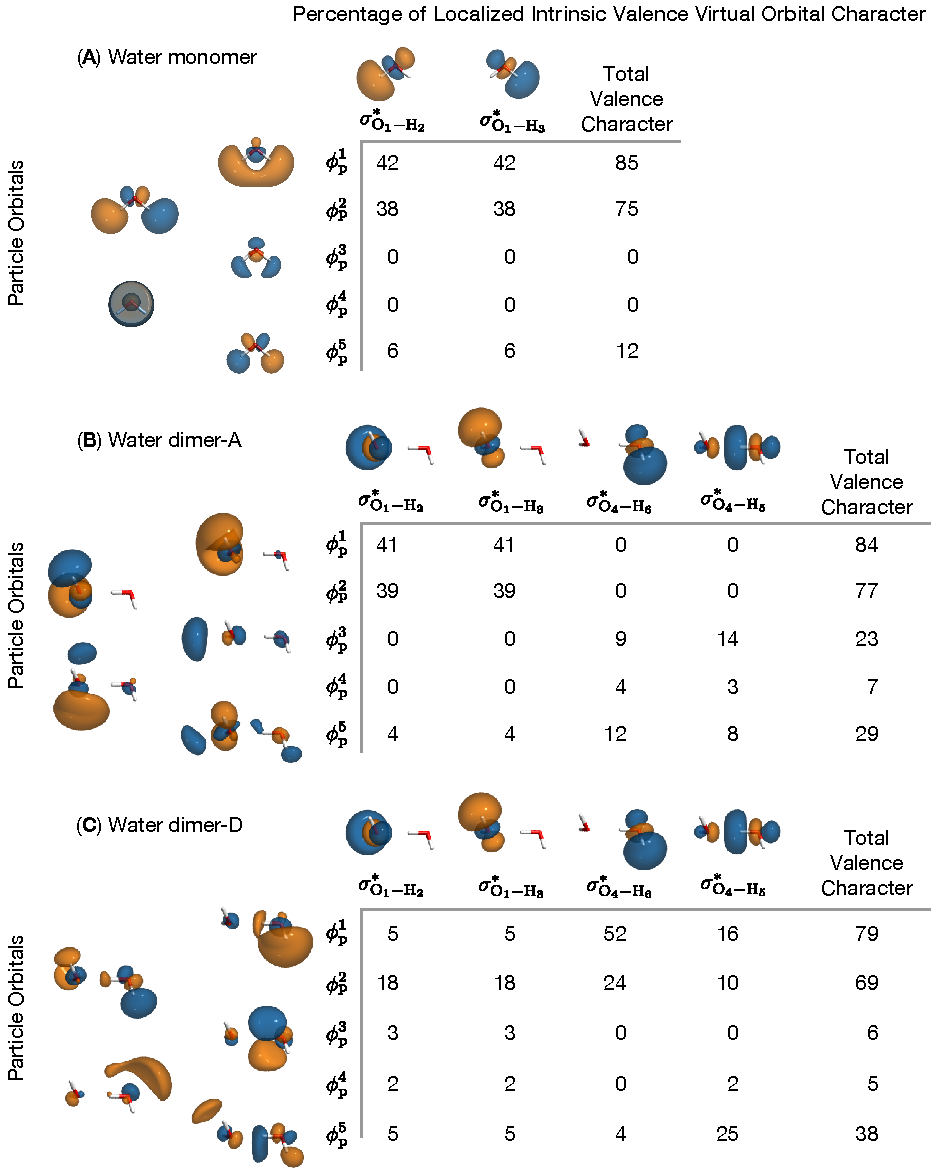
\includegraphics[width=5.75in]{figure_5_livvo_analysis_water.pdf}
\caption{Particle orbitals, valence virtual orbitals, and total valence character for each of the five core transitions in the NEXAFS spectrum of (A) water monomer, (B) the water dimer at the oxygen accepting the hydrogen bond, and (C) the water dimer at the oxygen donating the hydrogen bond.
Particle orbitals are numbered according to the calculated transitions reported in Table \ref{tab:water_spec} while atom numberings correspond to those shown in Figure~\ref{fig:water_spec}.}
\label{fig:water_all_livvo}
\end{figure*}

\textit{Water dimer, hydrogen bond donor}.
In contrast to dimer-A, the spectrum for dimer-D bears little resemblance to the monomer spectrum.
Although there are still three distinct peak features, the oscillator strength of all transitions drop significantly. We also observe a redshift of all three peaks, the first peak exhibits a mild shift of 0.2 eV while the higher energy peaks show more dramatic shifts of 0.7 and 1.0 eV respectively. The stark differences in the dimer-D spectrum, can be rationalized using our particle orbital/LIVVO analysis. The particle orbitals for each state shown in Figure~\ref{fig:water_all_livvo}C clearly show significant differences from the monomer spectrum for the dimer-D. The particle orbital for the first state in the dimer-D spectrum has similar orbital character to the first state in the monomer spectrum. However, $\phi_{\rm p}^1$ for dimer-D is clearly perturbed by the formation of the hydrogen bond and localizes along the free OH bond. 
This phenomenon has been observed in previous studies,\cite{fransson_requirements_2016,cavalleri_interpretation_2002} but the degree of localization has not been rigorously quantified. 

The LIVVO overlaps reported in Figure~\ref{fig:water_all_livvo}C for $\phi_{\rm p}^1$ shows that 52\% of the orbital character lies along the $\sigma^*_{\rm O_4-H_6}$ orbital with only 16\% localized along the hydrogen bond and 10\% of the orbital character coming from LIVVOs localized on the accepting water molecule. For $\phi_{\rm p}^2$, a similar localization is observed, however, a significantly higher percentage (36\%) of orbital character is accounted for by LIVVOs on the accepting water. This sharing of electron density with the accepting water molecule is indicative of the effect of hydrogen bonding on the dimer spectrum and has a direct correlation to the changes in intensity that we see in the simulated NEXAFS spectrum. Table \ref{tab:water_spec} shows a drop in $f_\mathrm{osc}$ when comparing the monomer to dimer-D, with a modest decrease for state 1 (0.00811 $\rightarrow$ 0.00605) and a far more drastic decrease for state 2 (0.01839 $\rightarrow$ 0.00878). This intensity drop can be attributed to delocalization of the particle orbital and correlates well with the population of LIVVOs on the accepting water molecule (10\% and 36\%, respectively).

In conclusion, LIVVOs help to address the origin behind the stark differences in the dimer-A and dimer-D spectra.
Perhaps the most revealing signature of hydrogen bonding in the water dimer is the decrease in intensity of the lowest two peaks in the dimer-D contribution.
Past studies have reasoned that the differences in these two spectra arise from the polarization of the orbitals in water.\cite{fransson_requirements_2016,cavalleri_interpretation_2002}
Due to the large dipole moment the virtual orbital are expected to be polarized toward the two hydrogen atoms and the NEXAFS spectrum will show more pronounced changes for the water molecule donating a hydrogen bond than for the one accepting it.
Our LIVVO analysis is consistent with this physical interpretation.
In addition, it quantifies the degree of delocalization of the particle orbitals in terms of localized valence orbitals.

\subsection{Basis Set Dependence of LIVVO Analysis}
An important aspect to address concerning this method is its dependence upon the choice of basis set. To fully address this issue, there are three aspects of the method that must be tested with respect to their basis set dependence: 1) How consistent are the LIVVO assignments, i.e. is there significant fluctuation in the LIVVO/IAO overlaps (eq \ref{eq:livvo_iao_overlap})? 2) Are the LIVVOs assigned to the excited state consistent? and 3) How much fluctuation is there in the particle orbital/LIVVO overlaps (eq \ref{eq:part_livvo_overlap})? We will address these three points in this section, using the two LIVVOs used to assign the first two excited states in ethanethiol, $\sigma^*_{\rm S^3-H^9}$ and $\sigma^*_{\rm S^3-C^2}$.

First we will take a look at the assignment of the atomic character of the LIVVOs, Table \ref{tab:basis_compare} shows the overlap of each VVO with eight of the IAOs in ethanethiol. These values are extremely consistent regardless of the choice of basis set, only deviating by a maximum of 0.01.

Next we will evaluate if the LIVVO assignments of the particle orbital are consistent for different basis sets. For ethanethiol, $\phi^1_{\rm p}$ was assigned primarily to the $\sigma^*_{\rm S^3-H^9}$ LIVVO with a weaker contribution from $\sigma^*_{\rm S^3-C^2}$ while $\phi^2_{\rm p}$ received a complementary assignment. Regardless of the choice of basis set, the LIVVO classification of both excited states is consistent. In all cases, $\phi^1_{\rm p}$ has greater than 57\% overlap with the  $\sigma^*_{\rm S^3-H^9}$ LIVVO and 25\% or less overlap with the $\sigma^*_{\rm S^3-C^2}$ LIVVO. Similarly, $\phi^2_{\rm p}$ has 57\% or greater overlap with $\sigma^*_{\rm S^3-C^2}$ and 25\% or less overlap with  $\sigma^*_{\rm S^3-H^9}$. The characterization of the orbital character of excited states is by far the most important feature of this technique, the consistency seen in the data across different basis sets is very encouraging. 

Lastly, we will address the consistency of the LIVVO/particle orbital overlap quantity presented in eq \ref{eq:part_livvo_overlap} with respect to choice of basis set. Table \ref{tab:basis_compare} shows that this value can potentially fluctuate $\pm$ 10\% with the choice of basis set. However, since we have shown that the formulation of the LIVVOs has a negligible dependence on the choice of basis set, we conclude that the basis set dependence seen in these values can solely be attributed to the basis set dependence of the particle orbitals.
Although these values can change fairly significantly, it is encouraging that they do not effect the overall interpretation of the excited state.

\begin{table*}[!t]
\centering
\footnotesize
\caption{Basis set dependence of the IAO assignment of LIVVOs and overlap [$\Omega_{\mathrm{p}l}^{(n)}$] of the $\sigma^*_{\rm S^3-H^9}$ and $\sigma^*_{\rm S^3-C^2}$ LIVVOs  with the first two particle orbitals of ethanethiol.}
\begin{tabular}{@{\extracolsep{6pt}}ccccccccccc@{}}
\toprule
LIVVO & $\psi^{\rm IAO}_{7}$(C$^2_{\rm s}$)& $\psi^{\rm IAO}_{9}$(C$^2_{\rm p}$)& $\psi^{\rm IAO}_{10}$(C$^2_{\rm p}$)& $\psi^{\rm IAO}_{13}$(S$^3_{\rm s}$) & $\psi^{\rm IAO}_{17}$(S$^3_{\rm p}$) & $\psi^{\rm IAO}_{18}$(S$^3_{\rm p}$) & $\psi^{\rm IAO}_{19}$(S$^3_{\rm p}$) &$\psi^{\rm IAO}_{25}$(H$^9_{\rm s}$) & $\Omega_{\mathrm{p}l}^{(1)}$ & $\Omega_{\mathrm{p}l}^{(2)}$ \\
\midrule
\multicolumn{11}{c}{\bf{cc-pVDZ}} \\
$\sigma^*_{\rm S^3-H^9}$ & 0.00 & 0.00 & 0.00 & 0.08 & 0.23 & 0.00 & 0.15 & 0.54 & 63.7 & 22.3 \\
$\sigma^*_{\rm S^3-C^2}$ & 0.09 & 0.33 & 0.09 & 0.07 & 0.00 & 0.32 & 0.09 & 0.00 & 22.6 & 67.1\\
\multicolumn{11}{c}{\bf{cc-pVTZ}} \\
$\sigma^*_{\rm S^3-H^9}$ & 0.00 & 0.00 & 0.00 & 0.08 & 0.22 & 0.00 & 0.15 & 0.54 & 59.3 & 23.9 \\
$\sigma^*_{\rm S^3-C^2}$ & 0.09 & 0.33 & 0.08 & 0.07 & 0.00 & 0.32 & 0.09 & 0.00 & 24.6 & 61.5\\
\multicolumn{11}{c}{\bf{cc-pVQZ}} \\
$\sigma^*_{\rm S^3-H^9} $& 0.00 & 0.00 & 0.00 & 0.08 & 0.22 & 0.00 & 0.15 & 0.54 & 57.8 &  22.8\\
$\sigma^*_{\rm S^3-C^2} $& 0.09 & 0.33 & 0.08 & 0.07 & 0.00 & 0.32 & 0.09 & 0.00 & 24.3 & 59.2\\
\multicolumn{11}{c}{\bf{aug-cc-pVDZ}} \\
$\sigma^*_{\rm S^3-H^9} $& 0.00 & 0.00 & 0.00 & 0.08 & 0.22 & 0.00 & 0.16 & 0.54 & 60.8 &  11.1\\
$\sigma^*_{\rm S^3-C^2} $& 0.09 & 0.33 & 0.08 & 0.07 & 0.00 & 0.32 & 0.09 & 0.00 & 15.3 & 63.1\\
\multicolumn{11}{c}{\bf{aug-cc-pVTZ}} \\
$\sigma^*_{\rm S^3-H^9} $& 0.00 & 0.00 & 0.00 & 0.08 & 0.22 & 0.00 & 0.15 & 0.54 & 57.9 &  14.7\\
$\sigma^*_{\rm S^3-C^2} $& 0.09 & 0.33 & 0.08 & 0.07 & 0.00 & 0.32 & 0.09 & 0.00 & 19.2 & 59.1\\
\multicolumn{11}{c}{\bf{aug-cc-pVQZ}} \\
$\sigma^*_{\rm S^3-H^9}$ & 0.00 & 0.00 & 0.00 & 0.07 & 0.23 & 0.00 & 0.16 & 0.54 & 56.5 & 15.7\\
$\sigma^*_{\rm S^3-C^2}$ & 0.08 & 0.33 & 0.09 & 0.07 & 0.00 & 0.32 & 0.09 & 0.00 & 20.4 & 57.3\\
\bottomrule
 \end{tabular}
 \label{tab:basis_compare}
 \end{table*}


\section{Conclusions}
In this work, we present an automated method for the characterization of core-valence excited states.
Our approach utilizes intrinsic atomic orbitals (IAOs) to derive a set of localized intrinsic valence virtual orbitals (LIVVOs) and assign their orbital character.
LIVVOs are in turn used to classify particle orbitals calculated using orthogonality constrained density functional theory (OCDFT).

For molecular orbitals with dominant valence character, this analysis provides keen insight into the localized $\sigma^*$  and $\pi^*$ orbitals that contribute to it.
For example, in the first two core excited states of ethanethiol, an electron is promoted to virtual orbitals that span both the S--C and S--H bonds. These contributions are difficult to discern by visual inspections of the MOs.
For the first state, our analysis shows that the particle orbital is dominated by the $\sigma^*_{\rm S^3-H^9}$ LIVVO (58\%) with a smaller contribution from the $\sigma^*_{\rm S^3-C^2}$ (22\%) LIVVO, revealing that this transition involves primarily the thiol bond.
Instead, for the second state we find that weights are reversed, with the $\sigma^*_{\rm S^3-C^2}$ LIVVO being the dominant contribution (57\%).

We have also shown how LIVVOs may be useful to quantify differences in excited states due to changes in the molecular environment.
For example, in the case of the water dimer we analyze the correlation between orbital localization due to hydrogen bonding and spectral features.
The NEXAFS spectrum of water dimer at the oxygen K-edge is known to have distinct contributions from the oxygens at water donating (dimer-D) or accepting (dimer-A) the hydrogen bond. 
Analysis of the two lowest particle orbitals for excitations on dimer-A show equal localization along intramolecular OH bonds.
However, the corresponding excitations for dimer-D are significantly different.
In the lowest energy state, 70\% of the electron is localized on the dimer-D, and this percentage decreases to 34\% in the second state.
These changes in degree of localization explain changes in intensity in the oxygen K-edge spectrum predicted by theory.

We have also considered the basis set dependence of the LIVVOs and the orbital analysis. Due to the robustness of the intrinsic atomic orbitals, the LIVVOs and our analysis of the orbital character are largely insensitive to the basis set size.

While our LIVVO analysis is applied here within the context of orthogonality constrained density functional theory, the method is general and can be used to decompose any set of virtual orbitals.
Overall, our LIVVO-based analysis of particle orbitals is a first step toward creating a general, robust, and automatic method to assign the character of excited states.

\newpage

\section*{Acknowledgments}
This work was supported by start-up funds provided by Emory University.
We would like to thank  Dr. Robert M. Parrish for kindly providing us with the implementation of intrinsic atomic orbitals in Psi4.
W.D.D. is supported by the National Science Foundation Graduate Research Fellowship under Grant No. 0000048655. Any opinion, findings, and conclusions or recommendations expressed in this material are those of the authors and do not necessarily reflect the views of the National Science Foundation.


{\footnotesize
\bibliography{refs}
\bibliographystyle{achemso}
}
\end{document}

\documentclass{article}
    % General document formatting
    \usepackage[margin=0.7in]{geometry}
    \usepackage[parfill]{parskip}
    \usepackage[utf8]{inputenc}
    \usepackage{graphicx}
    \usepackage{comment}
    \usepackage{notes2bib}
    \usepackage[sort&compress,numbers,super]{natbib}
    \usepackage{booktabs}
    
    % Related to math
    \usepackage{amsmath,amssymb,amsfonts,amsthm}
\begin{document}
\chapter{A Maximum Subspace Occupation Approach for the Study of the NEXAFS Spectra of Chemisorbed Organic Molecules Using Orthogonality Constrained Density Functional Theory: Pyrazine on Si(100) a Case Study}
\epigraph{\textit{``We may, I believe, anticipate that the chemist of the future who is interested in structures with high molecular weight will come to rely upon a new structural chemistry, involving precise geometrical relationships among the atoms in the molecules''}}{Linus C. Pauling}
\begin{chapabstract}
The near-edge X-ray absorption fine spectra (NEXAFS) at the carbon and nitrogen K-edge of pyrazine in the gas-phase and chemisorbed to the Si(100) surface are investigated using orthogonality constrained density functional theory (OCDFT). We introduce a novel approach for selectively target the 1s excitations of the adsorbate atoms based on atomic orbital subspace projection that allows for a priori specification of an atomic orbital subset relevant to the adsorbate. Using this approach we are able to simulate the NEXAFS spectrum of chemisorbed organic complexes at the K-edge of the adsorbate atoms. To analyze the calculated transitions we employ an orbital analysis based on localized intrinsic valence virtual orbitals (LIVVOs) in conjunction with OCDFT particle orbitals in order to provide a clear justification for every assignment.   Utilizing the LIVVO analysis we are able to quantify the amount of $\pi^*$/$\sigma^*$ mixing in each excited state and provide clear justification for changes in peak intensity.
\end{chapabstract}
\section{Introduction}
The adsorption of unsaturated hydrocarbons on the Si(100) surface has substantial technological significance: \cite{tao_electronic_2009,bent_organic_2002,filler_surface_2003} exposed surface silicon dimers react with organic molecules forming covalent Si-C bonds which alters the reactivity of the silicon surface and opens up the possibility of fabricating novel semiconductor based molecular devices. \cite{wolkow_controlled_1999,karthauser_control_2011,mentovich_multipeak_2008,joachim_electronics_2000} This promise has inspired considerable investigation into the fundamental mechanisms that drive the chemisorption process. \cite{mayne_chemisorbed_2004,lu_diradical_2003,taguchi_adsorbed_1991,sinniah_new_1989,zhao_temperature-programmed_2017,akagi_chemistry_2016} For this purpose, aromatic systems compose a particularly interesting class of molecules since their interaction with the surface often involves a myriad of unique bonding geometries that depend upon intrinsic properties such as the electronic and geometric structure of the molecule \cite{konecny_cycloaddition_1998,lu_chemisorption_2002,qu_theoretical_2004} as well as extrinsic factors like temperature, coverage, and pressure. \cite{tao_formation_2002,kong_nexafs_1998,wang_reactions_2003} Aromatic molecules that contain a heteroatom can cause notable modifications the adsorption process, for example nitrogen-containing molecules have additional configurations that involve the donation of the nitrogen lone-pair electrons to the silicon. \cite{romeo_n1s_2014,tao_dative_2003,miwa_selective_2005,weier_local_2011,ardalan_reactions_2011,chatterjee_self-directed_2013} This occurs in the case of the pyrazine (C$_4$H$_4$N$_2$) molecule, a six membered aromatic heterocycle with electronic properties similar to those of benzene and pyradine. The ring system contains two nitrogen atoms at opposite ends (\textit{para}), which increases the number of possible binding configurations upon molecular adsorption. \cite{lu_chemisorption_2002} Therefore the adsorption structure of pyrazine on the Si(100) surface is a very intriguing problem to study and has been the focus of many theoretical and experimental investigations. \cite{lu_chemisorption_2002,jung_adsorption_2009,huang_selective_2004,lee_selective_2012,lu_reactions_2002,ng_mechanism_2013,omiya_well-oriented_2012,shimomura_behaviour_2013}

\begin{figure}[b!]
\centering
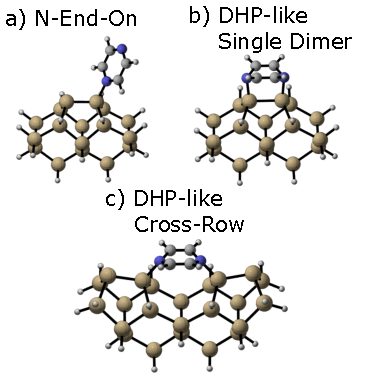
\includegraphics{structures.pdf}
\caption{Schematic of three unique absorption modes of pyrazine (C$_4$H$_4$N$_2$) on Si(100), a) one with a single N atom attached at the Si surface dimer, and two structures that form a 1,4-N-N-dihydropyrazine (DHP)-like structure through forming two covalent Si-N bonds on a b) single dimer or c) across two dimer rows.}
\label{fig:structures}
\end{figure}

High-resolution electron energy loss spectroscopy (HREELS) studies by Huang et al.\cite{huang_selective_2004} show that the adsorption of pyrazine on Si(100) occurs in a highly selective manner, directly bonding to the surface through the two \textit{para} nitrogen atoms to form a 1,4-N-N-dihydropyrazine (DHP)-like structure (Figure \ref{fig:structures}b) attached to a single Si dimer. Density functional theory (DFT) cluster model calculations\cite{lu_chemisorption_2002} make a case for the N-end-on adsorbed pyrazine (Figure \ref{fig:structures}a) at low temperatures, and a species that is di-$\sigma$-bonded through the 2 and 5 carbons at elevated temperatures. DFT periodic slab studies by Jung and Kang\cite{jung_adsorption_2009} reveal that an isolated pyrazine molecule can bind in either the N-end-on configuration or di-$\sigma$-bonded cross-row configuration (Figure \ref{fig:structures}c) with equal preference but at high coverages the cross-row structure dominates and can form a linear molecular chain across the silicon dimer rows. This suggestion of the formation of a one-dimensional (1D) molecular chain is also in accordance with room temperature scanning tunneling microscopy (STM) and photoelectron diffraction (PED) studies by Shimomura et al. \cite{omiya_well-oriented_2012} that suggests pyrazine forms this 1D molecular chain through a quasi-polymerization reaction through the Si dangling bonds. Pyrazine is one of the earliest examples of this type of self-assembled 1D molecular chain structure on a clean Si(100) surface.\cite{ng_mechanism_2013} This molecular assembly is particularly exciting in the case of pyrazine as it creates an ordered chain of planar C=C double bonds that could assist with further reaction at the semiconductor surface. 

Near-edge X-ray absorption fine structure (NEXAFS) spectroscopy is a powerful experimental technique to elucidate modifications induced on the electronic and geometric structure of a molecule upon adsorption to a surface. \cite{stohr_nexafs_1992,penner-hahn_x-ray_1999,garino_determination_2014,tourillon_electronic_1988} One of the powerful features of NEXAFS in application to this class of molecules lies in the angular dependence of the spectral features on the light polarization. By obtaining angle resolved spectra, one can glean useful information about the orientation of the molecule with respect to the surface. \cite{rosenberg_polarization-dependent_1986,shimoyama_evidence_2000,stohr_determination_1987} The fully-polarization resolved C K-edge spectrum of pyrazine on the surface of Si(100) was obtained by Han-Koo et al.\cite{lee_selective_2012}  at 300K and 2L coverage.\bibnote{This L stands for Langmuir, it is a standard unit to quantify exposure of a surface to a gaseous sample. The quantity is obtained by multiplying the pressure of the gas by the time of exposure.} Their analysis showed an angular dependence of the intensity of the $\pi^*$ resonance relating to the orbitals of the C=C double bonds, resulting in an average tilt angle of the adsorbate with respect to the surface of approximately $34 \pm 5^{\circ}$. This result coupled with data from X-ray Photoelectron Spectroscopy, effectively eliminates all possible adsorption configurations except for the DHP-like cross-row configuration (See Figure \ref{fig:structures}c). 

Analysis of the NEXAFS spectral features benefit greatly from a theoretical treatment.  Calculations can provide useful insight into the relationship between the spectral features and structure. \cite{triguero_calculations_1998} In this regard, NEXAFS simulations of adsorbed species are particularly challenging because they require an accurate description of the adsorbate/substrate geometry and the core excited states of large systems.\cite{romeo_n1s_2014,besley_time-dependent_2007,fronzoni_density_2012} Finite cluster models are often employed to represent the adsorbed system as they are particularly adept at modeling phenomena that are localized on the surface or within the bulk of a solid.\cite{besley_time-dependent_2007,de_francesco_tddft_2007,francesco_s_2009} Interaction between the adsorbate and substrate model causes overlap of their molecular orbitals (MOs) and induces a rehybridization of the valence level. The position and intensity of features in the core spectrum will show modifications relative to the free molecule and can thus capture the influence that the surface has on the local electronic structure of the adsorbing molecule. Prior NEXAFS simulations for benzene and pyridine on Si(100) have employed finite models with as few as 9 to as many as 21 Si atoms. \cite{coustel_pyridine_2012} The goal is to obtain an accurate description of the limited region around the adsorbate to capture the dominant effects on the NEXAFS spectrum due to the localization of core excited states near the core hole. Previous work by Rangan et al. has investigated the effect of increasing cluster size on the the core excitation spectrum of organic heterocycles adsorbed to Si(100). \cite{rangan_adsorption_2005,rangan_experimental_2005} These studies show that increasing the number of Si atoms in the cluster model had a very small effect on the resulting spectrum with regard to peak position and intensity. Recent work by Romeo et al. on pyridine/Si(100) compared the results of indepently optimized small clusters to larger clusters cut from periodic slab calculations. \cite{romeo_n1s_2014} These results highlighted differences in the individual polarized components of the spectrum, however, the effect on the total spectrum appears to be minimal. The computational efficiency and previous succesful applications of finite cluster models has motivated their use for modeling the surface geometry in the current study with the understanding that any potential long-range interactions of the adsorbate with the extended surface will be neglected.

%The application of NEXAFS to chemisorbed complexes of organic molecules on metal surfaces has proven to be very useful in the determination of structure and reactivity. \cite{seo_adsorption_2014,romeo_n1s_2014,lee_selective_2012,mayne_chemisorbed_2004,sohn_phenylacetylene_2007,feyer_adsorption_2010} Due to the importance of silicon-based electronic devices, the interaction of organic molecules with silicon surfaces has been the subject of a myriad of studies.\cite{jung_cycloaddition_2005,coustel_adsorption_2008,barriocanal_reactions_2000,bozack_chemical_1986,choi_cycloaddition_2002, reutzel_dissociative_2015} Research efforts in this field have lead to significant progress in conventional electronics as well as the development of novel electronic devices such as: complementary metal-oxide  semiconductor devices,\cite{ashwell_synthesis_2011} microelectronics \cite{yates_new_1998, bent_organic_2002},  and nonlinear optical devices \cite{lopinski_determination_1998}. Developments in this field are extremely encouraging, but further progress hinges upon advancing our fundamental understanding of the chemistry that takes place at the molecule/silicon interface. 

%The functional changes at the surface will depend upon the electronic and geometric structure alterations of the adsorbate due to its interaction with the surface. Near-edge X-ray absorption fine structure spectroscopy (NEXAFS)   has been an indispensible tool for detecting such surface modulations. \cite{mayne_chemisorbed_2004,sohn_phenylacetylene_2007,feyer_adsorption_2010} This technique employs tunable, high-resolution synchrotron radiation sources that gives the spectrum a rich structure. By investigating localized electronic transitions from core-orbitals, NEXAFS provides an atom specific probe of the electronic structure. Analysis of the NEXAFS spectrum of chemisorbed organic molecules is extremely useful in surface science applications because it provides a direct pathway to explore the local geometric structure and bonding characteristics of the adsorbate molecules, and can assist in answering fundamental questions about the electronic structure and reactivity of the adsorbate. For example, a study by Tetsuhiro Sekiguchi on formic acid (HCOOH) adsorbed on Si(100) deduced that formic acid is tilted away from the surface normal by about 21$^{\circ}$ $\pm$ 2$^{\circ}$ by investigating the incidence-angle-dependence of the C$_{\rm 1s}$ $\rightarrow$ $\pi^*$ peak in the spectrum. This tilted angle it forms at the surface is similar to the dihedral angle in silyl formate (H$_3$Si$-$OCHO) leading to the obvious conclusion that adsorbed formic acid should have similar electronic structure properties as silyl formate.\cite{ikeura-sekiguchi_adsorption_1999}

%The Si(100) surface undergoes a (2 $\times$ 1) reconstruction to form adjacent rows of exposed Si-Si dimers. Each dimer is $\sigma$-bonded with a small amount of $\pi$-bonding character, giving these weak dimers similar electronic properties to general alkenes. It has been shown that organic molecules can undergo cycloaddition reactions and Diels-Alder reactions at the Si surface similar to the way they would with a general alkene.\cite{konecny_theoretical_1997}  Upon formation of the Si-C bonds, the carbons rehybridize accordingly. This view of bonding at the silicon surface is supported by both theoretical \cite{liu_bare_1995,imamura_first-principles_1995} and experimental \cite{taylor_adsorption_1992, yoshinobu_adsorbed_1987, nishijima_adsorption_1987, li_stm_1997, teplyakov_dielsalder_1998} studies on different organic molecules. 

Aside from the treatment of the adsorbate/substrate geometry, computational approaches must calculate core excitation energies and properties in order to simulate the NEXAFS spectrum. The accuracy of calculated energies depends upon a reliable treatment of correlation, relaxation, and relativistic effects. Highly accurate many-body approaches have had considerable success in this area including coupled cluster theory,\cite{fransson_carbon_2013,besley_equation_2012,coriani_coupled-cluster_2012,coriani_asymmetric-lanczos-chain-driven_2012,myhre_near-edge_2016} configuration interaction,\cite{maganas_combined_2014,maganas_l-edge_2014,grimme_density_1996} and Green's-function approaches.\cite{wenzel_calculating_2014,wenzel_analysis_2015,wenzel_calculating_2014,wenzel_physical_2016} However, the computational cost associated with these methods limits their application to smaller systems. Considering the number of atoms necessary to construct cluster model surfaces it is desirable to consider methods that are computationally feasible for application to larger problems. Approaches that offer reduced computational cost include linear response time-dependent density functional theory (TDDFT),\cite{imamura_time-dependent_2006,besley_time-dependent_2007,lestrange_calibration_2015}  Hartree--Fock static exchange method, configuration interaction singles,\cite{asmuruf_calculation_2008} $\Delta$SCF, and real-time TD-DFT.\cite{lopata_linear-response_2012} We have recently proposed an alternative DFT based approach known as orthogonality constrained DFT (OCDFT)\cite{evangelista_orthogonality_2013} and have shown that it yields highly accurate core excitation energies.\cite{derricotte_simulation_2015,verma_predicting_2016} It is a $\Delta$SCF based Kohn--Sham DFT method which avoids variational collapse of the SCF solution by explicitly invoking an orthogonality constraint between the ground and excited states. Preliminary benchmark studies showed that OCDFT can accurately treat core excitations, providing absolute excitation energies that are more accurate than TDDFT.
%Multiple scattering $X_{\alpha}$ (MSX) methods have been widely applied to study both the discrete and continuum regions of the spectrum.\cite{horsley_structure_1985,hitchcock_carbon_1986,stohr_identification_1987,vaterlein_analysis_1998,vaterlein_orientation_2000,guo_multiple-scattering_1989,tang_multiple-scattering_1991} While MSX is popular for chemisorbed NEXAFS spectra calculations, it is limited in its accuracy in the discrete part of the spectrum. This problem stems from the fact that the implementation relies on the muffin-tin approximation.\note{F}{Add reference to muffin-tin approximation} DFT transition potential (DFT-TP) theory\cite{triguero_calculations_1998-1,triguero_calculations_1998,romeo_n1s_2014,rangan_experimental_2005} is a very popular method for predicting NEXAFS and X-ray emission spectra of chemisorbed systems and is touted to be more accurate than MSX in the discrete region. TDDFT calculations of these systems \note{F}{it is unclear what ''these systems'' stands for.  Do you mean chemisorbed species, Si-organics?}  have been performed. \cite{asmuruf_time_2008,de_francesco_s_2009,de_francesco_tddft_2007,besley_time-dependent_2007}

%However, standard density functionals yield poor quantitative core-valence excitation energies that are consistently underestimated with respect to experimental peak features. One of two approaches are routinely employed in order to correct the underestimated TDDFT spectrum: 1) the energy position of the spectrum is empirically shifted by the amount necessary to match the onset of the experimental spectrum \cite{de_francesco_s_2009,de_francesco_tddft_2007} or 2) the amount of Hartree--Fock exchange used in the functional is optimized based on results for a set of similar molecules.\cite{asmuruf_time_2008,besley_time-dependent_2007} More accurate excitation energies can be obtained by using a  variational Kohn--Sham/self-consitent field ($\Delta$KS/SCF) based approach.\cite{triguero_calculations_1998}  $\Delta$KS/SCF generally yields absolute excitation energies that are more accurate than those from TDDFT.  Moreover, it has been shown to be less dependent on the choice of the functional.\note{F}{This sentence needs a reference} However, variational DFT approaches are typically avoided for full spectral calculations due to the need to variationally optimize higher excited states by separate SCF calculations and the potential for variational collapse of the solution. $\Delta$KS/SCF can be improved upon by use of the maximum overlap method (MOM) for excited states. \cite{besley_self-consistent-field_2009}
	
Core excitation energies are calculated in OCDFT through the use of the constrained multiple hole particle (CMHP) algorithm. Similar to other excited state algorithms, CMHP is built to sequentially target excited state solutions starting from the lowest (highest) energy solution in a bottom-up (top-down) fashion. This presents an issue when targeting core excitations of organic adsorbates since the highest energy solutions are valence excitations and the lowest energy solutions are core excited states related to atomsof the cluster model. Thus, starting from either extrema requires the calculation of multiple unwanted solutions before reaching the adsorbate core. Having the ability to bypass these unwanted states and specifically target the core orbitals of the adsorbate is highly desirable.

%Recently we have introduced a method known as orthogonality constrained density functional theory (OCDFT) \cite{evangelista_orthogonality_2013} and shown that it yields highly accurate core excitation energies. \cite{derricotte_simulation_2015} The explicit orthogonality introduced between the ground and excited states guarantees that excited states calculated in OCDFT will not suffer from the problem of variational collapse.
%This feature allows to employ OCDFT for full spectral calculations.
%Nevertheless, computing the full NEXAFS spectrum of an adsorbed molecule presents a unique computational challenge for OCDFT because the standard implementation cannot target specific excited states.
%
%
%Within the context of the OCDFT algorithm for multiple core-valence states,\cite{derricotte_simulation_2015} excited states are obtained by a series of OCDFT computations, starting with excitations from the lowest core orbital and progressing toward higher ones.
%However, this approach does not allow to target specific excitations, which renders the computation of the NEXAFS spectrum of chemisorbed  molecules highly inefficient.


Strategies to target specific core orbitals of interest are routinely employed to circumvent algorithmic challenges that exist in the calculation of core excited states. These methods typically fall into the category of either restricted excitation window (REW) \cite{stener_time_2003,besley_time-dependent_2010,lopata_linear-response_2012} or energy-specific (ES) techniques. \cite{lestrange_calibration_2015,peng_energy-specific_2015}  These two methods differ by the way they solve the linear response equations. In the case of REW, the molecular orbital (MO) space from which excitations are allowed is restricted  using either an orbital energy cutoff or MO Mulliken populations. In ES methods, the linear response equations are solved in the full MO space targeting eigenvalues that lie above a predefined energy threshold. To the best of our knowledge, similar strategies for targeting specific excitations have not been explored within the context of variational DFT methods. 

Another theoretical challenge that is encountered by all methods is appropriately assigning transitions in chemisorbed complexes. Often times when classifying the NEXAFS spectra of gas-phase molecules it is sufficient to simply classify the transition as $\sigma$ or $\pi$, which can easily be done by inspecting the character of the molecular orbitals involved in the final state. In the case of chemisorbed molecules it is also important to specify which atoms are major contributors to the final state orbital. This is crucial, since a large part of interpreting chemisorbed spectra is deciphering which peak features are a result of interactions with the surface and which features are largely localized on the adsorbate. Determining this through simple inspection of the MOs can be ambiguous, and thus a more quantitative approach toward determining this is desirable.

In this paper we introduce a new approach for targeting core-excitations in adsorbed molecules within OCDFT based on an atomic orbital subspace occupation analysis. Using this method we can circumvent the algorithmic difficulty of calculating core excitations from multiple low lying surface atoms and specifically focus on the adsorbate atoms of interest. By developing this method around specification of atomic orbitals it requires little prior knowledge of the electronic structure of the molecule unlike other reduced subspace methods where exact energy ranges are required. We also address the issue of assigning transitions using a classification method based on localized intrinsic valence virtual orbitals.\cite{derricotte_localized_2017} We utilize these tools in order to analyze the NEXAFS spectrum of pyrazine chemisorbed on a Si(100) surface. 

%Despite the high volume of spectroscopy and imaging data available for these systems, there are examples of discrepancies in the NEXAFS literature concerning the origin of certain spectral features and/or the geometry on the surface. For acetylene, upon comparison to the gas-phase spectrum there is a significant shift of the reported $\pi^*_{\rm C-C}$ peak of about $-$1.2 eV. Experimentally this shift was attributed to the charge transfer from the Si dimer atoms to the C atoms upon formation of the Si-C bond.\cite{matsui_adsorption_2000} In contrast, a study by Besley and Noble attributes this shift solely to the lengthening of the C$-$C bond upon adsorption.\cite{besley_time-dependent_2007} In the case of benzene, two experimental NEXAFS studies were critical in the early stages of identifying the geometry on the Si(100) surface. However the two studies reached very different conclusions. The first study by Kong et al. \cite{kong_nexafs_1998} concluded that there were two unique structures present on the surface. While the study by Witkowski et al. \cite{witkowski_polarization_2003} performed 5 years later obtained a very different spectral profile and concluded that there is only one structure present on the surface. NEXAFS calculations done on this system since that time have yet to fully resolve why these spectra obtain vastly different results.\cite{besley_time-dependent_2007} In the years following these studies, a more sophisticated understanding of the structure of benzene at the Si(100) surface has been gained,\cite{lopinski_benzene/si100:_1998, lopinski_multiple_1998, silvestrelli_adsorption_2000, hofer_benzene_2001, kruse_gentle_2002, kim_coverage-dependent_2005,lee_conversion_2005, nisbet_local_2008, czekala_van_2014, coustel_mechanism_2014} and these new results warrant a fundamental reinterpretation of these crucial spectra. 
%\begin{figure}[!t]
%\centering
%\includegraphics{Benzene_structs.pdf}
%\caption{Stable structures of benzene on a double dimer Si(100) structure. All structures were optimized at the B3LYP/6-31G* level of theory.}
%\label{fig:benzene_structs}
%\end{figure} 

%Due to the possibility of multiple stable confirmations, the study of benzene adsorption on Si(100), must consider multiple binding possibilities. First principles studies have concluded six stable structures of the chemisorbed complex,\cite{silvestrelli_adsorption_2000,jung_cycloaddition_2005} these stable structures are shown in Figure \ref{fig:benzene_structs}. All structures contain at least two C-Si $\sigma$ bonds which effectively breaks the aromaticity of the benzene molecule. The single butterfly structure (SB) forms two C-Si bonds along a single Si dimer through C$_1$ and C$_4$ of the benzene ring. Two double bonds remain in tact in the structure and buckle upward away from the surface, yielding a C$-$C$-$Si angle of 104.6$^{\circ}$ on both sides of the Si dimer. The tilted structure (T) forms C-Si bonds across a single Si dimer at C$_1$ and C$_2$, leaving two conjugated double bonds in the molecule. The remaining portion of the molecule "tilts" away from the surface as a result of the C-Si bonding. The diagonal bridge butterfly structure (DBB) is similar to the SB structure however the C-Si bonds are formed across the two adjacent rows of Si dimers. The tight bridge (TiB) and twisted bridge (TwB) structures all form four C-Si bonds between C$_1$-C$_4$ leaving behind a single C$-$C double bond. They differ in the position of this double bond, in the TiB structure the double bond is parallel to the row of Si dimers while the TwB structure has this double bond perpendicular to the Si dimers. The pedestal structure has C-Si bonds formed at C$_1$, C$_2$, C$_4$, C$_5$ leaving the molecule lying relatively flat along the surface. This configuration leaves behind no double bonds and leaves unpaired electrons at C$_3$ and C$_6$. By coupling Carbon 1s photoelectron diffraction (PhD) studies with multiple scattering curved-wave calculations, Nisbet and coworkers\cite{nisbet_local_2008} were able to define a reliability factor $R_m$, and determine which configurations best correlated with the experimental modulation amplitudes:
%\begin{align}
%R_m = \frac{\sum^m_{i = 1} (\chi^i_{\rm th} - \chi^i_{\rm exp})^2}{\sum^m_{i = 1} (\chi^{i^2}_{\rm th} - \chi^{i^2}_{\rm exp})}
%\end{align}
%where $\chi^i_{\rm th} $ and $\chi^i_{\rm exp}$ are the theoretical and experimental modulation amplitudes respectively. Using this metric, it was determined that singlet-site simulations of the SB and TiB  structures yielded the best fits with reliability factors of 0.23 and 0.26 respectively. The T, P, TwB, and DBB structures yielded worse fits with $R$-factors of 0.63, 0.47, 0.45, and 0.35 respectively. This provided the necessary quantitative evidence to effectively exclude the TwB, T, P, and DBB structures as possible adsorption configurations of benzene on Si(100). Further simulations with a mixture of structures determined that the optimal $R$-factor is obtained with a 58\%:42\% mixture of SB and TiB. Other structure mixes were tried and all yielded a significantly higher $R$-factor. This rejects the possibility that there is only a single configuration present on the surface, and shows that the true surface geometry must consist of a mixture of SB and TB geometries. These results will help aid our discussion of the simulated OCDFT spectra of benzene.  

%In this work orthogonality constrained density functional theory is used to calculate the C K-edge of acetylene, ethylene, and benzene adsorbed on a Si(100) surface cluster model. In order to effeciently target the C K-edge we implement a reduced subspace technique in order to selectively target core-excitations from the C atoms of the organic adsorbate. Reduced subspace techniques are quite common in TDDFT in order to compute core-excitation energies and becomes necessary here as well in these unique cases. We also introduce a quantitative approach for determining which atoms are involved in the transition based on an atomic decomposition of the dipole moment. We will use these tools to analyze the NEXAFS spectra of gas-phase and chemisorbed acetylene, ethylene, and benzene and attempt to resolve some of the current controversies in the literature that exist about each chemisorbed spectrum. 

\section{Method}
\subsection*{Orthogonality Constrained Density Functional Theory}
OCDFT is a time-independent variational density functional method \cite{ayers_time-independent_2012} used to calculate electronic excited states. The original formulation of the theory can be found in ref \citenum{evangelista_orthogonality_2013}, while details on its extension to treat core excitations and the algorithm used to calculate multiple excited states to simulate full NEXAFS spectra can be found in ref \citenum{derricotte_simulation_2015}.  
%OCDFT is a variational time independent (TI) formulation of DFT that builds upon the approach developed by Ayers, Levy, and Nagy\cite{ayers_time-independent_2012}, where all $n$ electronic states $\Psi^{(n)}$ of an $N$-electron system have a unique corresponding density functional $E^{(n)}[\rho]$, which is a generalization of the ground state functional $E^{(0)}[\rho]$. The energy functional for state $n$ minimizes the expectation values of the energy while imposing that the trial wave function ($\Psi$) be compatible with the density ($\rho$) and  orthogonal to the first $n$ states: 
In OCDFT, a generalized Kohn--Sham picture is assumed, where to the $n^{\rm th}$ electronic state there exists an auxiliary system of noninteracting electrons with wave function $\Phi^{(n)}$ and density $\rho^{(n)}$ that corresponds to the real interacting system $\Psi^{(n)}$.
The wave function for the auxiliary system is a single Slater determinant, $\ket{\Phi^{(n)}} = \ket[1]{\phi_1^{(n)}\phi_2^{(n)} \cdots\phi_N^{(n)}}$, where the set of orbitals $\{\phi_i^{(n)}\}$ are different for each electronic state.

\begin{equation}
\label{eq:OCcondition}
\langle \Phi^{(m)} | \Phi^{(n)} \rangle = \delta_{mn} \;\;\;  \forall m,n
\end{equation}
 It can be shown, that given this constraint, one-electron excited states can be characterized by variationally optimized hole ($\phi_{\rm h}$) and particle ($\phi_{\rm p}$) orbitals, which must span the occupied and virtual spaces of the ground state wave function, respectively.
%\begin{equation}
%\hat{Q}^{(0)} \phi_{\rm h}^{(1)} = 0
%\label{eq:hole}
%\end{equation}
%\begin{equation}
%\hat{P}^{(0)} \phi_{\rm p}^{(1)} = 0
%\label{eq:particle}
%\end{equation}
%where $\hat{P}^{(n)}$ projects onto the occupied orbitals of state $n$,  $\hat{P}^{(n)} = \sum^{\rm occ}_i \ket[1]{\Phi_i^{(n)}} \bra[1]{\Phi_i^{(n)}}$, while $\hat{Q}^{(n)}$ is a projects onto the corresponding virtual space, such that $\hat{Q}^{(n)} + \hat{P}^{(n)} = 1$. Thus equations \ref{eq:hole} and \ref{eq:particle} can simply be interpreted as constraining the hole and particle orbitals to the occupied and virtual space of the ground state respectively. 
In this work we employ our constrained multiple hole/particle (CMHP) algorithm for the solution of multiple orthogonally constrained excited states.\cite{derricotte_simulation_2015} This allows us to readily compute multiple excited states by enforcing mutual orthogonality between the hole and particle orbitals of each subsequent excited state. At the same time, the CMHP scheme fully accounts for relaxation of all orbitals. 
\subsection*{Maximum Subspace Occupation}

%After enforcing the hole orthogonality condition in Equation \eqref{eq:hole} we obtain the following hole eigenvalue equation:
%\begin{align}
%\label{eq:one_state_hole_eq}
%\hat{P}^{(0)}(1-\hat{Q}_{\rm s}^{(1)}) \hat{f}^{(1)} (1-\hat{Q}_{\rm s}^{(1)})\hat{P}^{(0)} |\phi_{\rm h}^{(1)}\rangle &= \epsilon^{(1)}_{\rm h} |\phi_{\rm h}^{(1)}\rangle,
%\end{align}

%where $\hat{f}^{(1)} $ is the Kohn--Sham Hamiltonian of the excited state and $\hat{Q}_{\rm s}$ is the projector on to the virtual spectator space, i.e. the virtual orbitals that are not involved in the excitation ($\hat{Q}_{\rm s} = 1 - \hat{P} - \hat{Q}_{\rm h})$. The utility of Equation \eqref{eq:one_state_hole_eq} is to determine the hole orbitals and the hole eigenvalues ($\epsilon^{(1)}_{\rm h} $) which are ordered according to their energy. Previously we exploited this energy ordering to specifically target core excited states by simply by inverting the eigenvalue spectrum such that instead of choosing the highest energy orbitals (valence orbitals) we select the lowest energy orbitals (core orbitals).\cite{derricotte_simulation_2015} This allowed us to seemlessly calculate a series of orthogonally constrained core-excited states. This methodology works well for small molecules where there exists only a few atoms in the system. However for the case of chemisorbed organic molecules we encounter a unique challenge, the atoms involved in the surface model often times have lower energy core orbitals than the adsorbate atoms of interest. In the standard CMHP algorithm, core excitations from these lower energy core orbitals of the surface model must be considered first before the adsorbate core orbitals of interest, creating a situation that is computationally infeasible at worst and inefficient at best. 

Here we introduce our approach for selectively targeting the core excitations of interest by combining OCDFT with a scheme to target specific hole orbitals. We start by considering a set of atomic orbital (AO) basis functions $\varphi_{s}$ that are ordered by atom center, principal quantum number, and angular momentum. Based on this criteria, we can specify a subset of AO basis functions $s$ that are of interest in a given system. For NEXAFS K-edge applications this is going to be the 1s core orbital(s) centered on the atom(s) of interest. The specified basis functions can be used to build an operator ($\hat{\Gamma}_{s}$) that projects onto the AO subset.
%After building containing all occupied orbitals for a given system (\{$i$\}). In order to target the specific occupied orbitals of interest, we must build a truncated subspace of occupied orbitals (\{$\tilde{i}$\}) such that it contains only the core orbitals of interest. 
\begin{align}
\hat{\Gamma}_{s} = \sum_{s}\ket[1]{\varphi_{s}}\bra[1]{\varphi_{s}}
\end{align}
Utilizing this operator, we can evaluate the atomic orbital occupation number ($\Omega_i$) of each molecular orbital $\phi_i$ within the desired subspace.
\begin{equation}
\Omega_i = \bra[1]{\phi_i} \hat{\Gamma}_{S} \ket[1]{\phi_i} = \sum_{S} \braket[1]{\phi_i}{\varphi_{S}}\braket[1]{\varphi_{S}}{\phi_i}.
\label{eq:proj}
\end{equation}
This is a number between 0 (no occupation in the AO subset) and 1 (full occupation in the AO subset). We have implemented this maximum subspace occupation (MSO) scheme in OCDFT for the selection of the hole orbital. Now instead of being chosen from the full occupied set, the hole orbitals $\phi_{\rm h}$ are chosen from a subset of occupied orbitals $\phi_i$ with $\Omega_i \geq \omega$ where $\omega$ is a user-defined occupation threshold parameter. 
\begin{figure}
\centering
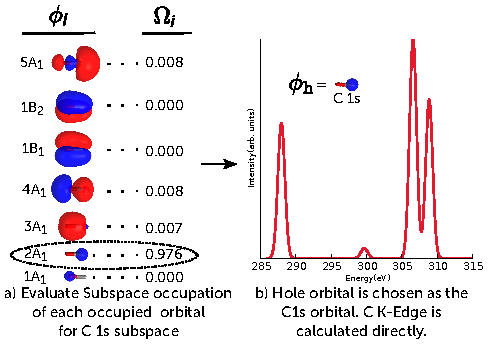
\includegraphics{CO_projection.pdf}
\caption{Example application of the maximum subspace occupation method within OCDFT to target the C 1s core excitations in CO at the B3LYP/3-21G level of theory: a) the 7 occupied orbitals of CO in C$_{2V}$ symmetry, with the corresponding subspace occupation number ($\Omega_i$) for a subspace composed of the C 1s atomic orbital. b) These projections are used to build the sebset of occupied orbitals, in this example a hole threshold of 0.2 is used, and thus orbital 2A$_1$ is chosen as the target hole orbital. This allows for direct access to the relevant C K-edge transitions.}
\label{fig:CO_projection}
\end{figure}
Figure \ref{fig:CO_projection} shows an example application of this subspace projection scheme to the calculation of carbon core excitations in carbon monoxide. In this example, the C$_{\rm 1s}$ $\rightarrow$ $\pi^*$ transition is targeted without needing to calculate any O$_{\rm 1s}$ excitations beforehand. This projection scheme which is based on the nature of the atomic orbital provides a distinct advantage to traditional REW and ES methods, as it requires no prior knowledge of the orbital energies or relevant energy range of absorption for a given system.

%\begin{table}
%\caption{Orbital overlap with subspace at different subspace specifications}
%\begin{tabular}{cccc}
%\hline
%\hline
%& \multicolumn{3}{c}{Requested Subspace} \\
%Orbital & [Cl(1s)] & [O(1s)] & [N(1s)] \\
%\hline
%1A(Cl$_{1 \rm s}$) & 0.9639 & 0.0000 & 0.0000\\
%2A(O$_{1 \rm s}$) &  0.0000 & 0.9793 & 0.0000\\
%3A(N$_{1 \rm s}$)  & 0.0000&  0.0000 & 0.9790\\
%\hline
%\hline
%\end{tabular}
%\end{table}

Table \ref{tab:CCl4} shows the first 3 carbon core excitations in a CCl$_4$ molecule calculated with and without the subspace projection method. Comparison of these two approaches shows a negligible difference between the excitation energies (less than 0.001 eV) and oscillator strengths. The case of targeting the C K-edge of CCl$_4$ is comparable in this sense to targeting the C K-edge of chemisorbed organics. In order to compute three transitions of the C K-edge using the standard algorithm, one must first compute twelve excited states related to the Cl K-edge (three for each Cl atom). However, when applying the subspace projection technique, the C 1s orbitals can be targeted in an efficient manner without the need to calculate any Cl core excitations. 

\begin{table}
\centering
\footnotesize
\caption{First 3 carbon core excitation energies and oscillator strengths (f$_{\rm osc}$) in a CCl$_4$ molecule calculated with and without the maximum subspace occupation (MSO) method in OCDFT. All calculations were performed using the B3LYP functional and aug-cc-pvdz basis set.}
\begin{tabular}{ccccc}
\hline
\hline
State & \multicolumn{2}{c}{OCDFT}& \multicolumn{2}{c}{MSO-OCDFT}  \\
\hline 
& $\omega$ (eV) & f$_{\rm osc}$ & $\omega$ (eV) & f$_{\rm osc}$ \\
\hline 
1 & 292.0002 & 0.0000 & 292.0005 & 0.0000\\
2 & 292.7093 & 0.0384 & 292.7097 & 0.0384 \\
3 & 292.6669 & 0.0385 & 292.6659 & 0.0385\\
\hline
\hline
\end{tabular}
\label{tab:CCl4}
\end{table}

\begin{comment}
\subsection*{Assigning Transitions Based on Atomic Decomposition}
Peak intensities for each electronic transition ($\Psi^{(n)}$ $\leftarrow$ $\Psi^{(0)}$) are approximated by the oscillator strength ($f_{\rm osc}$):
\begin{align}
f_{\rm osc} = \frac{2}{3} |\boldsymbol\mu_{n0}|^2 \omega_n
\end{align}
where $\omega_n$ is the excitation energy for state $n$ and $\boldsymbol\mu_{n0}$ is the transition dipole moment approximated in OCDFT as the expectation value of the KS determinants. 
\begin{align}
\boldsymbol\mu_{n0} = \langle \Phi^{(n)} | {\bf{\hat{r}}} | \Phi^{(0)} \rangle
\label{dipole}
\end{align}
where $\Phi^{(n)}$ is the $n$-th excited state and ${\bf{\hat{r}}}$ is the position operator. We conduct a Mulliken analysis of the transition dipole moment in order to make assignments of transitions based on their dominant atomic contributions. The transition dipole matrix elements can be rewritten in the atomic orbital basis ($\chi_{\mu}$) in the following fashion:
\begin{equation}
\boldsymbol\mu_{0n}  = \sum_{\mu\nu} D^{n0}_{\mu\nu} \bra{\chi_\mu} \hat{\mathbf{r}} \ket{\chi_\nu}
\end{equation}
where $D^{n0}_{\mu\nu}$ is the transition density matrix and $\bra{\chi_\mu} \hat{\mathbf{r}} \ket{\chi_\nu}$ is the transition dipole integral in the atomic orbital basis. Decomposing the total dipole moment in this way allows us to perform a restricted sum over discrete atomic contributions that have the same the angular momentum shell $l_A$ of donor atom A and shell $l_B$ on the acceptor atom B.
\begin{equation}
\label{eq:contribution}
\boldsymbol\mu_{n0} (\mathrm{B}_{l_\mathrm{B}} \leftarrow \mathrm{A}_{l_\mathrm{A}} ) = \sum_{\mu \in \mathrm{A}_{l_\mathrm{A}}}\sum_{\nu \in \mathrm{B}_{l_\mathrm{B}}} D^{0n}_{\mu\nu} \bra{\chi_\mu} \mathbf{r} \ket{\chi_\nu}
\end{equation}
Grouping atomic transitions by atom center and angular momentum enables the assignment of excitations based on which AOs are the most significant contributors to the total dipole moment. Classifying excitations in this way was found to be a very useful tool in evaluating the nature of core excited states of transition metal complexes. \cite{verma_predicting_2016}
\end{comment}
%For computations of chemisorbed molecules involving small surface cluster models, it has been shown that this can introduce intense spurious excitations to the cluster model that are unphysical and could cause discrepancy when comparing to experiment or gas-phase analogs. [CITE] To remedy this, it can also be advantageous to introduce a subspace of virtual orbitals such that only virtual orbitals with significant contributions from the adsorbate are included, to this end, we introduce a similar criterion based on a different subspace of basis functions $\{\tilde{\rho}\}$.
%\begin{align}
%\kappa^{\rm vir}_a = \sum_{\tilde{\rho}} |c_{\tilde{\rho} a}|^2
%\end{align}
%If $\kappa^{\rm vir}_a$ is greater than a user defined cutoff, then $a$ is included in a subspace of virtual orbitals \{$\tilde{a}$\}. Then during each excited state computation, the particle orbital is chosen to belong to this subspace of virtual orbitals. 
%\begin{align}
%\phi_p \in \{\tilde{a}\}.
%\end{align}
%This subspace routine is currently implemented in the OCDFT plugin in {\sc{psi4}}, the only additional input required is for the user to specify the atoms/orbitals that correspond to the hole and particle subspace and the occupied and virtual orbital cutoffs. 


\subsection{Assigning Transitions Based on Localized Intrinsic Valence Virtual Orbitals}
In this section, we summarize our method for classifying excited states based on a novel localized orbital representation known as the \textit{localized intrinsic valence virtual orbitals} (LIVVOs), only a brief summary is given here, for full details on this technique we refer the reader to Ref. \citenum{derricotte_localized_2017}. This unique set of orbitals is a special case of the valence virtual orbitals (VVOs) developed by Rudenberg and coworkers.\cite{lu_molecule_2004} The goal of VVOs is to obtain a more chemically meaningful orbitals through evaluation of the valence character of the canonical molecular orbitals. This is done by identifying an accurate atomic minimal basis set (AAMBS) and evaluating the overlap of the canonical virtual orbitals with the AAMBS functions $\psi^{\rm AAMBS}_{\rho}$ such that:
\begin{equation}
(\mathbf{S})_{a\rho} = \langle \phi_a | \psi^{\rm AAMBS}_{\rho} \rangle.
\end{equation}
For our implementation we have chosen to use the intrinsic atomic orbitals of Kinizia \cite{knizia_intrinsic_2013} as the necessary AAMBS functions. Following the suggestion of Ref. \citenum{schmidt_valence_2015} a singular value decomposition (SVD) is performed on $\mathbf{S}$:
\begin{equation}
\mathbf{S} = \mathbf{U} \mathbf{\sigma} \mathbf{V}^{\dagger}
\end{equation}
to yield the orthogonal transformation matrices $\mathbf{U}$ and $\mathbf{V}$. These are rotations of the canonical virtual space and the AAMBS space, respectively that bring the two orbital sets into maximum coincidence. The transformation matrix $\mathbf{U}$ is then applied to the virtual set in the following way:
\begin{equation}
|\psi^{\rm VVO}_{\nu} \rangle = \sum_{a}^{N_{\rm vir}} |\phi_a \rangle U_{a\nu}, \nu = 1,2,...,N_{\rm VVO}
\end{equation}
where $N_{\rm vir}$ is the number of virtual orbitals while $N_{\rm VVO}$ is the number of VVOs. Finally, the set of LIVVOs ($\psi^{\rm LIVVO}_l$) are formed by using Pipek-Mezey localization,\cite{pipek_fast_1989} we arrive as a set of localized VVOs that span the antibonding interactions of the molecular environment.

For every excited state in OCDFT, we analyze the character of the particle orbital $\phi^{(n)}_{\rm p}$ by evaluating its overlap with each LIVVO:
\begin{equation}
\Omega^{(n)}_{\rm{p}l} = |\langle \phi^{(n)}_{\rm p}|\psi^{\rm LIVVO}_l \rangle|^2
\end{equation}
The individual overlaps $\Omega^{(n)}_{\rm{p}l}$ are used to assign the character of the particle orbital to the $l$-th LIVVO. In addition, we also define the total valence character $t^{\rm val,(n)}_{\rm p}$ for any given particle orbital as the sum of its overlap with all LIVVOs:
\begin{equation}
t^{\rm val, (n)}_{\rm p} = \sum_l^{N_{\rm LIVVO}} \Omega^{(n)}_{\rm pl}.
\end{equation}
With this set of orbitals it is possible to quantify the most important local contributions to the particle orbitals to provide a specific description of its character to make a robust assignment for the excited state.
\section{Computational Details}
The gas-phase geometry of pyrazine was optimized using the B3LYP \cite{becke_new_1993,lee_development_1988,vosko_accurate_1980,stephens_ab_1994} functional and the 6-31G*\cite{rassolov_6-31g*_1998,hariharan_influence_1973,francl_selfconsistent_1982} basis set.  All core excited states were calculated using OCDFT in the PSI4 \textit{ab-initio} quantum chemistry package.\cite{turney_psi4:_2012} Core excited state calculations on the free molecule were done at the PBE/cc-pVTZ\cite{perdew_generalized_1996,dunning_gaussian_1989} level of theory. Pyrazine is then attached in the double dimer bridging configuration to a Si$_{23}$H$_{24}$ cluster model of the Si(100) surface reconstruction. Covalent Si-N bonds are formed between adjacent dimer rows and the \textit{para} nitrogen atoms of pyrazine. Core excitation calculations on chemisorbed pyrazine utilize the PBE functional\cite{perdew_generalized_1996} and a custom basis set where the cc-pVTZ basis set\cite{dunning_gaussian_1989} is used for all carbon and hydrogen atoms and the 6-31G basis set\cite{hehre_selfconsistent_1972} for all silicon atoms. The AO subspace is chosen as the C 1s or N 1s orbitals to simulate their respective K-edges with a hole threshold of 0.2. This threshold ensures that the only hole orbitals chosen are MOs corresponding to carbon core orbitals. 

\begin{comment}
\begin{table*}
\caption{First two acetylene core excitations calculated on growing sizes of silicon clusters. All structures were optimized at the B3LYP/6-31G* level of theory, core excitations were calculated at the B3LYP levelusing the cc-pVTZ basis set for C and H atoms and 6-31G basis set for Si atoms. We have reported the most dominant atomic transition and its respective total transition dipole contribution.}
\begin{tabular}{ccccc}
\hline
\hline
Cluster & Transition& Energy (eV) & $f^{\rm abs}_{\rm osc}$ & $|\mathrm{A}_{l_\mathrm{A}} \rightarrow \mathrm{B}_{l_\mathrm{B}} |_{\rm max}$ \\
\hline
\vspace{0.2cm}\\
\multirow{2}{*}{\raisebox{-0.7cm}[0.5cm][0.5cm]{\includegraphics[width=0.1\textwidth, height=0.1\textwidth]{si9_ace.pdf}}} & $\pi^*_{\rm C-C}$ & 284.31 & 0.0204 & C$_{\rm s}$ $\rightarrow$ C$_{\rm p}$\\
 & $\sigma^*_{\rm C-Si}$ & 285.80 & 0.0065 & C$_{\rm s}$ $\rightarrow$ Si$_{\rm p}$\\
\vspace{0.2cm}\\
\multirow{2}{*}{\raisebox{-0.6cm}[0.5cm][0.5cm]{\includegraphics[width=0.1\textwidth, height=0.1\textwidth]{si15_ace.pdf}}} & $\pi^*_{\rm C-C}$ & 284.35 & 0.0199 & C$_{\rm s}$ $\rightarrow$ C$_{\rm p}$ \\
 & $\sigma^*_{\rm C-Si}$ & 285.72 & 0.0063 & C$_{\rm s}$ $\rightarrow$ Si$_{\rm p}$ \\
 \vspace{0.2 cm}\\
\multirow{2}{*}{\raisebox{-0.6cm}[0.5cm][0.5cm]{\includegraphics[width=0.1\textwidth, height=0.1\textwidth]{si21_ace.pdf}}}& $\pi^*_{\rm C-C}$ & 284.25 & 0.0196 & C$_{\rm s}$ $\rightarrow$ C$_{\rm p}$ \\
 & $\sigma^*_{\rm C-Si}$ & 285.71 & 0.0038 & C$_{\rm s}$ $\rightarrow$ Si$_{\rm p}$ \\
 \hline
 \hline
\end{tabular}
\label{tab:Cluster_Extend}
\end{table*}
\end{comment}
We note that pyrazine is a highly symmetrical molecule containing symmetry equivalent C and N atoms. Molecules that contain symmetry equivalent cores present a challenging theoretical issue.\cite{ma_breaking_1989,carravetta_symmetry_2013} In practice, symmetry restricted calculations produce a core hole that is delocalized evenly amongst all symmetry equivalent atoms. In contrast, a symmetry unrestricted calculation may produce core holes that are localized on each individual atom. For calculations on the free pyrazine molecule, we have studied both the symmetry restricted and unrestricted solutions. To obtain a state where the core hole is localized on each atom we utilize a wavefunction with broken spatial and spin symmetry by mixing the coefficients of the alpha HOMO and LUMO orbitals of pyrazine. 

For spectral simulations, the peak intensities are based on the oscillator strength ($f_{\rm osc}$):
\begin{equation}
f_{\rm osc} = \frac{2}{3}|\mu_{n0}|^2 \omega_n
\end{equation}
where $\mu_{n0}$ represents the transition dipole moment for transition from the ground state to excited state $n$ and $\omega_n$ is the excitation energy for that transition. The spectrum is simulated by centering Gaussian functions at each excitation energy with a peak height scaled by the oscillator strength of that transition. The peak is then broadened by a constant value in order to simulate natural spectroscopic broadening effects, for the purpose of pyrazine we utilized a Gaussian width of 0.3 eV. 
\section{Results and discussion}

%\subsection*{Gas-Phase}

%Figure \ref{gas_phase} shows the calculated C K-edge spectra for acetylene, ethylene, and benzene. The OCDFT excitation energies agree well with the experimental peak positions, with the largest error being 1.0 eV in the $\sigma_{\rm C-H}$ state of benzene. The experimental spectral profile of all three molecules are characterized by an intense feature in each spectrum that is a transition from C$_{1s}$ $\rightarrow$ $\pi^*$ orbitals.\cite{hitchcock_carbon_1977} Our calculated spectrum reproduces this very well, validating the accuracy of the oscillator strengths calculated in OCDFT.





%\begin{figure*}
%\centering
%\includegraphics{all_three_spectra_gas_phase.pdf}
%\caption{Calculated Near-edge X-ray absorption spectra for a) acetylene, b) ethylene, c) and benzene calculated with OCDFT at the B3LYP/cc-pvtz level of theory. Spectra were simulated by calculating 10 unique carbon core-excitations for each carbon atom. Transitions are convoluted with gaussians of FWHM=0.5 eV.}
%\label{gas_phase}
%\end{figure*} 

%First it is important to consider the gas-phase spectra of acetylene, ethylene, and benzene. These results will be important to consider in order to compare with the chemisorbed complexes and fully understand what happens to the NEXAFS spectra of the molecules upon chemisorption. The OCDFT gas-phase acetylene C K-edge shown in Figure \ref{gas_phase}a is characterized by three distinct peak features at 285.6, 288.6, and 290.9. This agrees well with the experimental peak positions at 285.9, 288.1, and 290.1. Figure  \ref{gas_phase_particles} shows the relevant particle orbitals for each assignment. Analysis of the particle orbital is used to distinguish between $\pi$ and $\sigma$ orbitals and determine the bonding or antibonding nature of the orbitals. Table \ref{tab:gas_phase_tab} shows the maximum atomic contribution for each transition, this analysis in conjunction with the analysis of the particle orbitals allow us to assign these peak as $\pi^*_{\rm C-C}$, $\sigma^*_{C-H}$, and $\sigma_{C-H}$ respectively.

%The C K-edge of ethylene shown in Figure \ref{gas_phase}b is similar in structure to the spectrum of acetylene with three distinct spectral features at 284.6, 288.2, and 290.4 eV, we have assigned these peaks as $\pi^*_{\rm C-C}$, $\sigma_{C-H}$, and $\sigma^*_{C-H}$ respectively. The onset of the K-edge at 284.6 eV is within 0.1 eV of the experimental onset representing excellent agreement with experiment. An error of about 0.8 eV is observed with the second peak compared to experiment, while the third peak has an error of 0.3 eV. 

%The benzene spectrum in Figure \ref{gas_phase}c is characterized by 3 peaks located at 285.2, 288.2, and 289.4 eV, we assign these peaks as $\pi^*_1$, $\sigma_{\rm C-H}$, and $\pi^*_2$. The spectral profile is fundamentally unique due to the presence of a second $\pi^*$ transition at higher energy, unlike the $\sigma$ states that are always much lower in intensity, the second $\pi^*$ state is nearly as intense as the first with a peak ratio between the two of 0.84. The onset of our calculated spectrum matches perfectly with the experiment at 285.2 with errors of 1.0 and 0.4 eV for the two higher lying peaks. Overall between the 9 excitations considered across these three molecules we have a mean average error of 0.5 eV, this is commensurate with the performance OCDFT has demonstrated with calculating carbon core excitations. 


%The structure of the NEXAFS spectrum for ethylene is shown in Figure \ref{gas_phase}b is similar to that of acetylene but with the higher energy transitions having higher oscillator strength relative to the $\pi^*$ peak, which is undoubtedly due to the presence of the extra C$-$H bond at each carbon. Experimentally, the C$_{1s}$ $\rightarrow$ $\pi^*$ transition occurs at 284.7 eV this is represented well in OCDFT with the $\pi^*$ transition occuring exactly at 284.7 eV. Our calculated spectrum predicts a C$_{1s}$ $\rightarrow$ $\sigma_{\rm C-H}$ transition at 287.8 eV, which agrees well with the  experimental assignment at 287.4 eV. The sharp resonance at 289.7 eV corresponds to a transition to a $\sigma^*_{\rm C-H}$ orbital, this transition is observed experimentally at 290.1 eV.

%\begin{figure}
%\centering
%\includegraphics{gas_phase_particles.png}
%\caption{Particle orbitals ($\phi_{\rm p}$) from the Near-edge X-ray absorption spectra for acetylene, ethylene, and benzene calculated with OCDFT at the B3LYP/cc-pvtz level of theory.}
%\label{gas_phase_particles}
%\end{figure} 

%For the benzene NEXAFS spectrum shown in Figure \ref{gas_phase}c, our calculated spectrum predicts a sharp $\pi^*$ resonance at 285.1 eV which agrees well with the experimental onset of 285.2 eV. The next peak at 286.9 eV arises due to transitions to $\sigma_{\rm C-H}$ orbitals, experimentally this transition is observed at 287.2 eV. We observe a 3p transiton at 289.0 eV which agrees exactly with the assignment and position of the experimental spectrum. A final $\pi^*$ transition is observed experimentally at 290.0 eV, and is shown here in the OCDFT spectrum at 290.3 eV.


%\begin{table}
%\footnotesize
%\begin{tabular}{cccc}
%\hline
%\hline
%exp. (eV) & OCDFT (eV) & f$_{\rm osc}$ & $|\mathrm{A}_{l_\mathrm{A}} \rightarrow \mathrm{B}_{l_\mathrm{B}} |_{\rm max}$\\
%\hline
%\multicolumn{4}{c}{\bf Acetylene} \\
%285.9 & 285.6 & 1.00000 & Cs $\rightarrow$ Cp \\
%288.1 & 288.6 & 0.36676 & Cs $\rightarrow$ Hs \\
%290.1 & 290.9 & 0.13065 & Cs $\rightarrow$ Hs \\
%\multicolumn{4}{c}{\bf Ethylene} \\
%284.7 & 284.6 & 1.00000 & Cs $\rightarrow$ Cp \\
%\multirow{2}{*}{287.4} & 287.8 & 0.21167 & Cs $\rightarrow$ Hs \\
%& 288.2 & 0.57038 & Cs $\rightarrow$ Hs \\
%290.1 & 290.4 & 0.19067 & Cs $\rightarrow$ Hs \\
%\multicolumn{4}{c}{\bf Benzene} \\
%285.2 & 285.2 & 1.00000 & Cs $\rightarrow$ Cp \\
%\multirow{2}{*}{287.2} & 287.8 & 0.27782 & Cs $\rightarrow$ Hs \\
%& 288.2 & 0.42899 & Cs $\rightarrow$ Hs \\
%289.0 & 289.4 & 0.84341 & Cs $\rightarrow$ Cp \\
%\hline
%\end{tabular}
%\label{tab:gas_phase_tab}
%\end{table}


%Overall, for all three molecules OCDFT agrees very well with the experimental peak positions, assignments, and intensities. This is not surprising considering we have seen excellent performance from OCDFT in the calculation of core-excited states in gas-phase organic molecules in recent benchmarks. 

\subsection*{NEXAFS Spectrum of Gas-Phase Pyrazine}
In this section we present an OCDFT simulation of the carbon and nitrogen 1s excitation spectrum for the free pyrizine molecule. Figure \ref{fig:free_pyrazine_nexafs} shows the experimental and calculated NEXAFS spectrum along with corresponding peak labels. The relevant particle orbitals and the LIVVOs used to characterize each excited state are shown in Figure \ref{free_pyrazine_parts_livvos}. Calculated excitation energies, oscillator strengths, and assignments are shown in Table \ref{tab:free_pyrazine_energy}. 

\begin{figure}[t!]
\centering
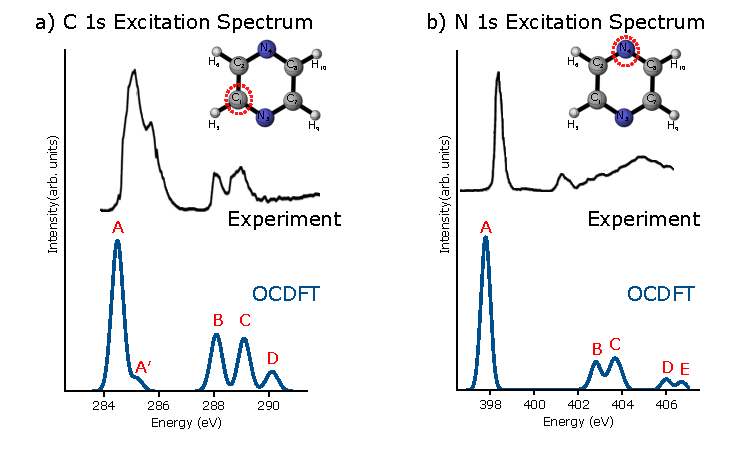
\includegraphics{pyrazine_nexafs_gas.pdf}
\caption{Near-edge X-ray absorption spectrum of pyrazine (C$_4$H$_4$N$_2$) at the a) C K-edge and b) N K-edge computed with OCDFT (blue line) at the PBE/cc-pVTZ level of theory. Experimental results (black line) are obtained from Ref. \citenum{vall-llosera_c_2008} and appear here in their original peak position with no applied energy shifts. The pyrazine geometry optimized at the B3LYP/6-31G* level is shown in the inset, the atoms circled (C$_1$ and N$_4$) are the core holes considered in further discussion of the results in this section.}
\label{fig:free_pyrazine_nexafs}
\end{figure}

Pyrazine, similar to other unsaturated molecules, follows a common pattern to their core excitation spectrum, a dominant edge onset associated with a $\pi^*$ resonance localized near the core hole followed by a series of weaker transitions that are a mix of $\sigma^*$ transitions, Rydberg transitions, and $\pi^*$ transitions localized away from the core hole. The experimental C 1s spectrum shown in Figure \ref{fig:free_pyrazine_nexafs}a follows this general trend. The Experimental spectrum is characterized by four main peaks at 285.3, 285.8, 288.2, and 289.1 eV. The simulated spectrum using OCDFT agrees well with corresponding peak features at 284.5, 285.2, 288.1, and 289.1 eV respectively. 

\begin{table}[t!]
\centering
\footnotesize
\caption{Calculated (PBE/cc-pVTZ) core excitation energies, oscillator strengths, and LIVVO assignments for the C and N 1s excitation spectrum of free pyrazine. The LIVVO assignments shown are the two with the highest percentage overlap with the particle orbital. For each calculated transition we report the $\pi^*$/$\sigma^*$ mixing ratio (see text for details) and the spectral feature that this state contributes to (see Figure \ref{fig:free_pyrazine_nexafs}). }
\begin{tabular}{cccrccc}
\hline
\hline
State & energy (eV) & osc & LIVVO Assignments & $\pi^*$/$\sigma^*$ Mixing & $t_{\rm p}^{\rm val}$ & Peak Contribution \\
\hline
\multicolumn{7}{c}{\bf C 1s Core Excitations} \\
1 & 284.5 & 0.0207 &  $78.2\%\pi^*_{\rm C_1-N_3} $ & 100\%$\pi^*$ & 97.9\% & A \\
& & & $19.3\%\pi^*_{\rm C_7-C_8}$ & & \\
2 & 285.2 & 0.0020 & $51.1\%\pi^*_{\rm C_1-N_3}$ & 100\%$\pi^*$ & 97.3\% & A$^{\prime}$ \\
& & & $43.9\%\pi^*_{\rm C_7-C_8}$ & & \\
3 & 288.1 & 0.0083 & $45.4\%\sigma^*_{\rm C_1-H_5}$ & 100\%$\sigma^*$ & 64.1\% & B \\
& & & $12.0\%\sigma^*_{\rm C_7-H_9}$ & & \\
4 & 289.1 & 0.0042 & $28.6\%\pi^*_{\rm N_3-C_7}$ & 65\%$\pi^*$/35\%$\sigma^*$ & 76.4\% & C\\
& & & $7.4\%\sigma^*_{\rm C_1-H_5}$ & & \\
5 & 289.1 & 0.0041 & $26.0\%\pi^*_{\rm C_7-C_8}$ & $61\%\pi^*$/$39\%\sigma^*$ & 74.6 & C \\
& & & $7.9\%\sigma^*_{\rm C_1-H_{5}}$ & & \\
6 & 289.4 & 0.0003 & $25.7\%\sigma^*_{\rm C_2-H_6}$ & $100\%\sigma^*$ & 54.0 & C \\
& & & $14.6\%\sigma^*_{\rm C_7-H_{9}}$ & & \\
7 & 290.1 & 0.0027 & $20.5\%\sigma^*_{\rm C_1-N_3}$ & $100\%\sigma^*$ & 59.5 & D \\
& & & $12.8\%\sigma^*_{\rm C_2-N_4}$ & & \\
8 & 290.2 & 0.0037 & $17.4\%\sigma^*_{\rm C_8-H_{10}}$ & $100\%\sigma^*$ & 49.9 & D \\
& & & $13.7\%\sigma^*_{\rm C_7-H_9}$ & & \\
\multicolumn{7}{c}{\bf N 1s Core Excitations} \\
1 & 397.8 & 0.0211 &  $59.4\%\pi^*_{\rm C_2-N_4}$ & 100\%$\pi^*$ & 98.4\% & A \\
& & & $34.8\%\pi^*_{\rm C_1-N_3}$ & & \\
2 & 399.3 & 0.0000 & $60.3\%\pi^*_{\rm C_7-N_8}$ & 100\%$\pi^*$ & 96.9\% & \\
& & & $22.2\%\pi^*_{\rm N_4-C_8}$ & & \\
3 & 402.4 & 0.0003 & $19.3\%\sigma^*_{\rm C_2-H_6}$ & 100\%$\sigma^*$ & 64.1\% & B \\
& & & $19.3\%\sigma^*_{\rm C_8-H_{10}}$ & & \\
4 & 402.8 & 0.0042 & $38.3\%\pi^*_{\rm C_1-N_3}$ & $88\%\pi^*$/$12\%\sigma^*$ & 85.4 & B \\
& & & $6.0\%\sigma^*_{\rm C_2-H_{6}}$ & & \\
5 & 403.2 & 0.0010 & $17.9\%\sigma^*_{\rm C_8-H_{10}}$ & 29\%$\pi^*$/71\%$\sigma^*$ & 58.7\% & C\\
& & & $8.9\%\pi^*_{\rm C_1-N_3}$ & & \\
6 & 403.6 & 0.0034 & $21.6\%\sigma^*_{\rm C_2-N_4}$ & $100\%\sigma^*$ & 68.3 & C \\
& & & $21.6\%\sigma^*_{\rm N_4-C_8}$ & & \\
7 & 403.8 & 0.0001 & $13.2\%\sigma^*_{\rm C_7-H_9}$ & $100\%\sigma^*$ & 59.5 & D \\
& & & $12.9\%\sigma^*_{\rm C_1-H_5}$ & & \\
8 & 403.9 & 0.0024 & $16.0\%\sigma^*_{\rm C_1-H_{5}}$ & $100\%\sigma^*$ & 52.4 & D \\
& & & $15.6\%\sigma^*_{\rm C_7-H_9}$ & & \\
\hline
\end{tabular}
\label{tab:free_pyrazine_energy}
\end{table}

The OCDFT spectrum for the C K-edge was calculated considering excitations from carbon atom C$_1$ (see inset in Figure \ref{fig:free_pyrazine_nexafs}), due to the symmetry of the molecule, it is obvious that the equivalent carbon cores, would produce an identical core excitation spectrum. Limiting our discussion to a single core also aides in our discussion of localization when analyzing our LIVVO assignments. The first peak A in the carbon 1s spectrum occurs at 284.5 eV with a small shoulder feature A$^{\prime}$ ocuring at 285.2 eV. These features can both be attributed to $\pi^*$ transitions that are a combination of the $\pi^*_{\rm C_1-N_3}$ and $\pi^*_{\rm C_7-C_8}$ LIVVOs. In the case of Peak A, 78.2\% of the particle orbital can be attributed to $\pi^*_{\rm C_1-N_3}$ which is localized near the core hole on atom C$_1$. On the contrary, the particle orbital for the shoulder feature A$^{\prime}$ only 51.1\% of the particle orbital can be attributed to $\pi^*_{\rm C_1-N_3}$, while 43.9\% is attributed to $\pi^*_{\rm C_7-C_8}$ which is localized away from the core hole. The calculated oscillator strength is sensitive to this change in localization, with state 1 having an oscillator strength of 0.0207 and state 2 having an oscillator strength of 0.0020. State 3 is the sole contribution to Peak B, with an excitation energy of 288.1 and an orbital character that can be assigned as  $\sigma^*_{\rm C_1-H_5}$.

\begin{figure}[t!]
\centering
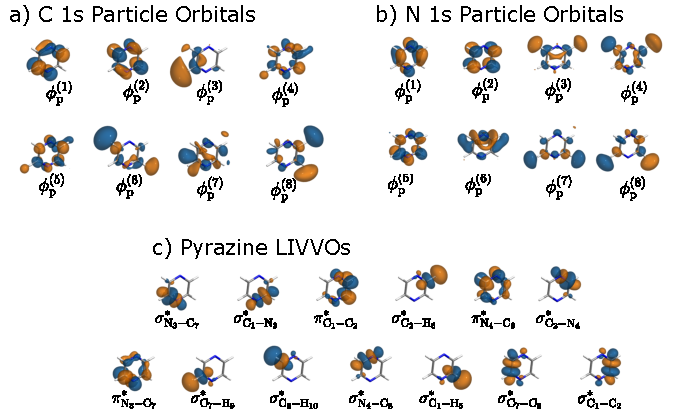
\includegraphics{pyrazine_gas_parts_and_Livvos.pdf}
\caption{Particle orbitals for the core excited states that contribute to the a) carbon and b) nitrogen 1s excitation spectrum. Also shown are c) the LIVVOs that are used to analyze the particle orbitals.}
\label{free_pyrazine_parts_livvos}
\end{figure}

States 3 and 4 are quasi-degenerate both yielding excitation energies of 289.1 eV. Looking at their particle orbitals $\phi^{(4)}_{\rm p}$ and $\phi^{(5)}_{\rm p}$ in Figure \ref{free_pyrazine_parts_livvos}, it is clear that they are orbitals of mixed $\pi^*$ and $\sigma^*$ character. This orbital mixing was noted in a previous study\cite{vall-llosera_c_2008} however never quantified in any manner, using the LIVVO analysis we are able to quantify this orbital mixing, this data is shown in Table \ref{tab:free_pyrazine_energy}. State 4 is 65\% $\pi^*$ and 35\% $\sigma^*$, while state 5 is 61\% $\pi^*$ and 39\% $\sigma^*$. This similarity in the composition of their orbital character explains the similarities between their energy and oscillator strength. A weak transition ascribed to a $\sigma^*_{\rm C_2-H_6}$ at 289.4 eV also contributes to Peak C. States 7 and 8 compose peak D at 290.1 and 290.2 eV. They are assigned to $\sigma^*_{\rm C_1-N_3}$ and $\sigma^*_{\rm C_8-H_{10}}$ respectively.

The N 1s core excitation spectrum shown in Figure \ref{fig:free_pyrazine_nexafs}b shows a similar general structure to the C 1s spectrum. Peak A occurs at 397.8 eV and can be assigned to $\pi^*_{\rm C_2-N_4}$ which is the $\pi^*$ orbital localized near the core hole. Interestingly, state 2, which has an excitation energy of 399.3 eV has an oscillator strength of zero providing no contribution to the spectrum. The LIVVO analysis shows that 60.3\% of this partical orbital can be attributed to the $\pi^*_{\rm C_7-N_8}$ orbital, which is localized away from the nitrogen core hole at N$_4$. Also, the particle orbital $\phi^{(2)}_{\rm p}$ shown in Figure \ref{free_pyrazine_parts_livvos} shows that the orbital has no contribution localized at the nitrogen atoms. State 3 is a small contribution to Peak B at 402.4 eV attributed evenly to $\sigma^*_{\rm C_2-H_6}$ and \sigma^*_{\rm C_8-H_{10}}$. As with State 2, much of the orbital character is localized away from the nitrogen resulting in a much weaker transition. As seen in the C 1s spectrum, States 4 and 5 are of mixed $\pi^*$ and $\sigma^*$ character. However, unlike the mixed states in the C spectrum, the composition of these orbitals in the N spectrum are unique. State 4, which contributes to Peak B at 402.4 eV, contains 88\% $\pi^*$ character and only 12\% $\sigma^*$ character. This state is assigned primarily to the $\pi^*_{\rm C_1-N_3}$ orbital localized near the core hole, resulting in an appreciable oscillator strength of 0.0042. Although State 5 is also a mixed state it contains far more $\sigma^*$ character, with only 29\% $\pi^*$ character and 71\% $\sigma^*$ character. This state can be assigned to the $\sigma^*_{\rm C_8-H_{10}}$ LIVVO, which explains its weak intensity in the N 1s spectrum. State 6 is a more intense contribution to Peak C at 403.6 eV and is assigned to $\sigma^*_{\rm C_2-N_4}$ and $\sigma^*_{C_8-N_4}$, the two C-N $\sigma$-bonds assciated with the core hole N atom. States 7 and 8 contribute to Peak D at 403.8 and 403.9 eV respectively and are composed of transitions to $\sigma^*$ orbitals associated with C-H bond along the ring system.

\begin{figure}[b!]
\centering
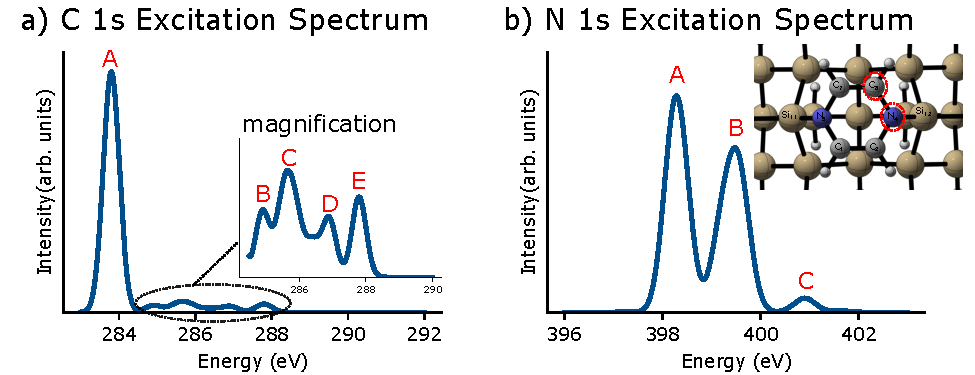
\includegraphics{pyrazine_chemisorbed_c_kedge.pdf}
\caption{Near-edge X-ray absorption spectrum of pyrazine (C$_4$H$_4$N$_2$) chemisorbed on a Si$_{23}$H$_{24}$ cluster model of Si(100) at the a) C K-edge and b) N K-edge computed with OCDFT at the PBE level. All C, N, and H atoms use the cc-pVTZ basis set while the 6-31G basis set is used for the Si atoms of the cluster model. The inset in the C spectrum magnifies the $\sigma^*$ manifold of the spectrum. The pyrazine geometry optimized at the B3LYP/6-31G* level is shown in the inset in the N spectrum, the atoms circled (C$_8$ and N$_4$) are the core holes considered in further discussion of the results in this section.}
\label{fig:chem_pyrazine_nexafs}
\end{figure}

\subsection*{NEXAFS Spectrum of Chemisorbed Pyrazine on Si(100)}
The OCDFT simulated NEXAFS spectrum of pyrazine chemisorbed on the Si(100) surface is shown in Figure \ref{fig:chem_pyrazine_nexafs}. The LIVVOs shown in Figure \ref{fig:chem_pyrazine_livvos} are only those that are directly involved with the adsorbed pyrazine molecule. In total, this system produces 70 LIVVOs however many of these are $\sigma^*_{\rm Si-Si}$ and  $\sigma^*_{\rm Si-H}$ orbitals related to the Si(100) cluster model. When comparing the LIVVOs of the chemisorbed complex to that of free pyrazine, many of the orbitals are remain unchanged except for  three critical differences. First, the most obvious difference is the appearance of the $\sigma^*_{\rm N_3-Si_{11}}$ and $\sigma^*_{\rm N_4-Si_{12}}$ LIVVOs to reflect the covalent bonds formed between the cluster and the para nitrogens on pyrazine. Secondly, the $\pi$ system of the molecule has changed and the LIVVOs reflect that, the $\pi^*$ orbitals are not localized along the N-C bonds, as is the case in free pyrazine, they are now localized along each C=C double bond with clear contributions from the N lone pair electrons. Lastly the $\sigma^*_{\rm Si_{13}-Si_{14}}$ represents the dangling bonds that exist at each open Si site on the dimers. These changes in the character of the LIVVOs gives us some insight into the effect of the cluster on the adsorbate. 

\begin{figure}[b!]
\centering
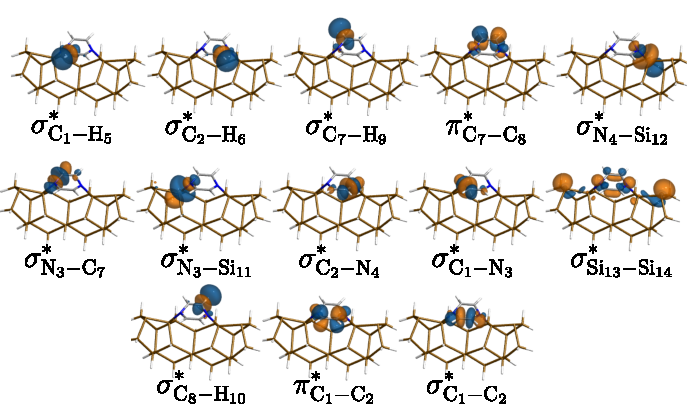
\includegraphics{pyrazine_chem_livvos.pdf}
\caption{LIVVOs used to analyze particle orbitals in pyrazine (C$_4$H$_4$N$_2$) chemisorbed on a Si$_{23}$H$_{24}$ cluster model of Si(100).}
\label{fig:chem_pyrazine_livvos}
\end{figure}

Since pyrazine maintains two double bonds upon binding on the surface, the NEXAFS spectrum can be expected to maintain the same general spectral pattern of a sharp $\pi^*$ peak and a weaker $\sigma^*$ manifold. The experimental NEXAFS spectrum of chemisorbed pyrazine reports the initial spectral feature at 285.9 attributed to a $\pi^*$ excitation. Our results show an initial excitation at 279.4 eV that is attributed to a $\sigma^*_{\rm Si_{13}-Si_{14}}$, which is the orbital associated with he open Si atoms. The appearance of this state in our calculations is purely an artifact of the cluster model. In reality, pyrazine forms a 1D molecular chain along the surface, leaving few open Si sites on the surface and thus quenching this state. State 2 at 283.8 eV agrees well with the experimental onset feature, is assigned to $\pi^*$ LIVVVOs, and is the sole contribution to Peak A in the spectrum. Considering the core hole at atom C$_8$ State 2 is localized heavily toward the core hole, with 73.4\% of the orbital character attributed to the $\pi^*_{C_7-C_8}$ LIVVO, this is similar to the localization along a single $\pi^*$ bond seen in the gas phase spectrum where the first state had 78.2\% overlap with a single $\pi^*$ LIVVO. The similarity between the LIVVO localization of the $\pi^*$ state in the gas and condensed phases considered here shows that the localization of this $\pi^*$ state is not significantly affected upon adsorption to the surface. Due to this, there is a large difference in intensity at the C K-edge of chemisorbed pyrazine between the $\pi^*$ peak and the $\sigma^*$ manifold, that didn't exist in the spectrum of free pyrazine. The crucial difference here is the interaction and subsequent rehybridization of the pyrazine valence orbitals with the Si cluster. Looking at the particle orbital $\phi^{(2)}_{\rm p}$ it is clear that this initial $\pi^*$ state interacts very little with the Si cluster, meanwhile every other particle orbital has significant contribution from Si cluster orbitals. This can also be seen quantitatively by looking at the LIVVO assignments in Table \ref{tab:chem_pyrazine_states}, for the $\pi^*$ state (State 2), a single VVO constitutes 76\% of the total valence character, in contrast no other state has a single VVO contribution of over 20\%. As a result, the $\sigma^*$ manifold for the C 1s spectrum is orders of magnitude less intense than the $\pi^*$ feature. 



The N 1s spectrum shown in Figure \ref{fig:chem_pyrazine_nexafs}b, does not show the same stark contrast in intensity as the C spectrum. This is due to the fact that the $\pi^*$ orbitals are now localized away from the N atoms upon the formation of the covalent Si-N bonds. In fact, in contrast to all other spectra considered here, the pure $\pi^*$ state (State 10) is the highest in energy at 401.6 eV and has an oscillator strength of zero. Interestingly this is not the only state to provide no intensity to the spectrum. States 6 and 7 also provide no intensity to the spectrum due to their interaction with the cluster, both states have no contributions from LIVVOs that are localized on the pyrazine molecule and their respective particle orbitals in Figure \ref{fig:chem_pyrazine_parts}b ($\phi^{(6)}_{\rm p}$ and $\phi^{(7)}_{\rm p}$) clearly shows no interactions from pyrazine. 

\begin{figure}[t!]
\centering
\includegraphics{n_and_c_chem_particles.pdf}
\caption{Particle orbitals for the core excited states that contribute to the a) carbon and b) nitrogen 1s excitation spectrum of pyrazine (C$_4$H$_4$N$_2$) chemisorbed on a Si$_{23}$H$_{24}$ cluster model of Si(100).}
\label{fig:chem_pyrazine_parts}
\end{figure}

Peak A of the N 1s spectrum has contributions from States 1 and 2, similar to the C 1s spectrum this first state is an artifact of the cluster from the open Si sites. State 2 however is a contribution from the Si-N bond, $\phi^(2)_{\rm p}$ has 39.7\% overlap with the $\sigma^*_{\rm N_4-Si_{12}}$ LIVVO. Peak B has contributions from States 3 and 4 both of which are mixed $\pi^*$/$\sigma^*$ states. Similar to the C 1s spectrum, this ratio favors $\sigma^*$ character due to interaction with the cluster model. The sole contribution to Peak C is a weak transition attributed to the $\pi^*$ orbitals with 5.2\% overlap with $\pi^*_{\rm C_7-C_8}$ and 4.9\% overlap with $\pi^*_{\rm C_1-C_2}$.  

\begin{table}
\centering
\footnotesize
\caption{Calculated (PBE/cc-pVTZ) core excitation energies, oscillator strengths, and LIVVO assignments for the C and N 1s excitation spectrum of pyrazine (C$_4$H$_4$N$_2$) chemisorbed on a Si$_{23}$H$_{24}$ cluster model of Si(100). The LIVVO assignments shown are the two with the highest percentage overlap with the particle orbital. For each calculated transition we report the $\pi^*$/$\sigma^*$ mixing ratio (see text for details) and the spectral feature that this state contributes to (see Figure \ref{fig:chem_pyrazine_nexafs}). }
\begin{tabular}{cccS[]ccc}
\hline
\hline
State & energy (eV) & osc & \rm \centering LIVVO Assignments & $\pi^*/\sigma^*$ Mixing & $t_{\rm p}^{\rm val}$ & Peak Contribution \\
\hline
\multicolumn{7}{c}{\bf C 1s Core Excitations} \\
1 & 279.4 & 0.0002 & 83.8\% $\sigma^*_{\rm Si_{13}-Si_{14}}$ & 1\% $\pi^*$/99\%$\sigma^*$ & 98.2\% & \\
2 & 283.8 & 0.0210& 73.4\% $\pi^*_{\rm C_7-C_8}$ & 86\% $\pi^*$/24\%$\sigma^*$ & 97.0\% & A \\
 & & & 10.5\% $\pi^*_{\rm C_1-C_2}$ & & & \\
 3 & 284.9 & 0.0005 & 11.8\% $\sigma^*_{\rm N_3-Si_{11}}$ & 100\%$\sigma^*$ & 92.2\% & B \\
 & & & 10.1\% $\sigma^*_{\rm N_4-Si_{12}}$ & & & \\
  4 & 285.3 & 0.0002 & 18.5\% $\pi^*_{\rm C_1-C_2}$ & 21\%$\pi^*$/79\%$\sigma^*$ & 92.2\% & C \\
 & & & 13.2\% $\sigma^*_{\rm N_3-Si_{11}}$ & & & \\
  5 & 285.6 & 0.0006 & 9.7\% $\pi^*_{\rm C_1-C_2}$ & 12\%$\pi^*/88\%$\sigma^*$ & 89.5\% & C \\
 & & & 4.0 \% $\sigma^*_{\rm C_8-H_{10}}$ & & & \\
       6 & 285.8 & 0.0005 & 11.4\% $\pi^*_{\rm C_7-C_8}$ & 14\%$\pi^*/86\%$\sigma^*$ & 89.9\% & C \\
 & & & 5.7 \% $\sigma^*_{\rm N_3-Si_{11}}$ & & & \\
   7 & 286.4 & 0.0003& 10.5\% $\sigma^*_{\rm C_8-H_{10}}$ & 100\%$\sigma^*$ & 87.2\% & D\\
 & & & 1.7 \% $\sigma^*_{\rm N_3-Si_{11}}$ & & & \\
    8 & 286.3 & 0.0000 & 2.1\% $\pi^*_{\rm C_7-C_8}$ & 3\%$\pi^*/97\%$\sigma^*$ & 91.0\% & D \\
 & & & 0.6\% $\pi^*_{\rm C_7-C_8}$ & & & \\
   9 & 286.9 & 0.0005 & 13.3\% $\sigma^*_{\rm C_8-H_{10}}$ & 2\%$\pi^*/98\%$\sigma^*$ & 83.9\% & D \\
 & & & 1.6\% $\sigma^*_{\rm C_7-H_9}$ & & & \\
    10 & 287.8 & 0.0007 & 12.0\% $\sigma^*_{\rm N_4-Si_{12}}$ & 4\%$\pi^*/96\%$\sigma^*$ & 89.9\% & E \\
 & & & 3.7 \% $\sigma^*_{\rm N_4-C_8}$ & & & \\
 \multicolumn{7}{c}{\bf N 1s Core Excitations} \\
     1 & 398.2 & 0.0026 & 85.1\% $\sigma^*_{\rm Si_{13}-Si_{14}}$ & 1\%$\pi^*/99\%$\sigma^*$ & 98.7\% & A \\
 & & & 1.3 \% $\sigma^*_{\rm N_4-Si_{12}}$ & & & \\
       2 & 398.4 & 0.0016 & 39.7\% $\sigma^*_{\rm N_4-Si_{12}}$ & 2\%$\pi^*/98\%$\sigma^*$ & 93.3\% & A \\
 & & & 2.1 \% $\sigma^*_{\rm N_4-C_8}$ & & & \\
        3 & 399.2 & 0.0010 & 12.3\% $\sigma^*_{\rm N_3-Si_{11}}$ & 15\%$\pi^*/85\%$\sigma^*$ & 92.8\% & B \\
 & & & 7.6 \% $\pi^*_{\rm C_7-C_8}$ & & & \\
         4 & 399.5 & 0.0010 & 11.0\% $\pi^*_{\rm C_7-C_8}$ & 22\%$\pi^*/78\%$\sigma^*$ & 92.2\% & B \\
 & & & 6.3 \% $\sigma^*_{\rm N_3-Si_{11}}$ & & & \\
           5 & 399.6 & 0.0005 & 9.9\% $\sigma^*_{\rm N_3-Si_{11}}$ & 12\%$\pi^*/88\%$\sigma^*$ & 89.9\% & B \\
 & & & 5.5 \% $\pi^*_{\rm C_7-C_8}$ & & & \\
            6 & 399.7 & 0.0003 & 5.6\% $\sigma^*_{\rm N_3-Si_{11}}$ & 5\%$\pi^*/95\%$\sigma^*$ & 89.9\% & B \\
 & & & 2.3 \% $\pi^*_{\rm C_7-C_8}$ & & & \\
             7 & 400.2 & 0.0000 & N/A & 100\%$\sigma^*$ & 91.3\% &  \\
          8 & 400.5 & 0.0000 & N/A & 100\%$\sigma^*$ & 91.3\% & \\
                       9 & 400.9 & 0.0003 & 5.2\% $\pi^*_{\rm C_7-C_8}$ & 12\%$\pi^*/88\%$\sigma^*$ & 87.8\% & C \\
 & & & 4.9 \% $\pi^*_{\rm C_1-C_2}$ & & & \\
      10 & 401.6 & 0.0000 & 44.2\% $\pi^*_{\rm C_1-C_2}$ & 87\%$\pi^*/13\%$\sigma^*$ & 95.7\% & \\
 & & & 38.9 \% $\pi^*_{\rm C_7-C_8}$ & & & \\
\hline
\end{tabular}
\label{tab:chem_pyrazine_states}
\end{table}
%To help understand what happens to the NEXAFS spectra of the molecules upon chemisorption it is important to first consider the core-excitations in gas-phase acetylene, ethylene, and benzene. Table \ref{tab:gas_phase_tab} shows the calculated core-excitation energies, oscillator strengths, and dominant atomic transitions of all three molecules in the gas-phase. Due to the presence symmetry equivalent carbon atoms in each molecule, we perform broken symmetry OCDFT calculations in order to obtain a solution with a localized core hole. When compared to the experimental peak positions, OCDFT has a mean average error of 0.5 eV across the 9 transitions considered in these three molecules, representing excellent agreement with experiment. This degree of accuracy is commensurate with previous OCDFT studies on gas-phase organic molecules.\cite{derricotte_simulation_2015,verma_predicting_2016} Our consideration of the atomic contributions to the electronic dipole moment along with the OCDFT particle orbitals help facilitate the assignments shown in Table \ref{tab:gas_phase_tab}. For more information on the gas-phase particle orbitals and simulated spectra for all three molecules in the gas-phase we refer the reader to the Supporting Information. 

%\begin{table}
%\footnotesize
%\caption{Calculated core-excitation energies, oscillator strengths, and dominant atomic transitions ($|\mathrm{A}_{l_\mathrm{A}} \rightarrow \mathrm{B}_{l_\mathrm{B}} |_{\rm max}$) for acetylene, ethylene, and benzene calculated with OCDFT at the B3LYP/cc-pVTZ level of theory. Spectra were simulated by calculating 10 unique carbon core-excitations for each carbon atom in the molecule. Only transitions shown here are non-redundant transitions with a relative oscillator strength of 0.1 or higher}
%\begin{tabular}{cccc}
%\hline
%\hline
%exp. (eV)[\citenum{hitchcock_carbon_1977}] & OCDFT (eV) & f$_{\rm osc}$ & $|\mathrm{A}_{l_\mathrm{A}} \rightarrow \mathrm{B}_{l_\mathrm{B}} |_{\rm max}$\\
%\hline
%\multicolumn{4}{c}{\bf Acetylene} \\
%285.9 & 285.6 & 1.00 & C$_{\rm s}$ $\rightarrow$ C$_{\rm p}$ \\
%288.1 & 288.6 & 0.37 & C$_{\rm s}$ $\rightarrow$ H$_{\rm s}$ \\
%290.1 & 290.9 & 0.13 & C$_{\rm s}$ $\rightarrow$ H$_{\rm s}$ \\
%\multicolumn{4}{c}{\bf Ethylene} \\
%284.7 & 284.6 & 1.00 & C$_{\rm s}$ $\rightarrow$ C$_{\rm p}$ \\
%\multirow{2}{*}{287.4} & 287.8 & 0.21 & C$_{\rm s}$ $\rightarrow$ H$_{\rm s}$ \\
%& 288.2 & 0.57 & C$_{\rm s}$ $\rightarrow$ H$_{\rm s}$ \\
%290.1 & 290.4 & 0.19 & C$_{\rm s}$ $\rightarrow$ H$_{\rm s}$ \\
%\multicolumn{4}{c}{\bf Benzene} \\
%285.2 & 285.2 & 1.00 & C$_{\rm s}$ $\rightarrow$ C$_{\rm p}$ \\
%\multirow{2}{*}{287.2} & 287.8 & 0.28 & C$_{\rm s}$ $\rightarrow$ H$_{\rm s}$ \\
%& 288.2 & 0.43 & C$_{\rm s}$ $\rightarrow$ H$_{\rm s}$ \\
%289.0 & 289.4 & 0.84 & C$_{\rm s}$ $\rightarrow$ C$_{\rm p}$ \\
%\hline
%\hline
%\end{tabular}
%\label{tab:gas_phase_tab}
%\end{table}

%\begin{table}
%\begin{tabular}{cccl}
%\hline
%\hline
%State &Energy (eV) & $f_{osc}$ & LIVVO Assignment \\
%\hline
%1 & 284.1 &  0.0019 & 85.9\% $\sigma^*_{\rm Si-N-C-Si}$ \\
%2 & 286.0 &  0.0189 & 77.3\% $\pi^*_{\rm C_1-C_2}$\\
%& & & 8.9\% $\pi^*_{\rm C_3-C_4}$ \\
%3 &287.4 &  0.0007 & 10.1\% $\sigma^*_{\rm N_1-Si}$ \\
%& & & 10.1\% $\sigma^*_{\rm N_2-Si}$ \\
%4 & 288.4 &  0.0009 & 8.5\% $\sigma^*_{\rm C_3-C_4}$\\
%& & & 7.0\% $\pi^*_{\rm C_3-C_4}$ \\
%5 & 287.8 &  0.0000 & 13.8\% $\pi^*_{\rm C_3-C_4}$ \\
%& & & 12.3\% $\sigma^*_{\rm N_2-Si}$ \\
 %\hline
 %\end{tabular}
%\end{table}

%\subsection*{Acetylene and Ethylene}
%The OCDFT calculated C K-edge of chemisorbed acetylene shown in Figure \ref{fig:all}a is characterized by three distinct spectral features at 284.3, 285.8, and 287.5 eV. The lowest energy peak feature at 284.3 is classified as $\pi^*_{\rm C-C}$ due to the $\pi^*$ character of the particle orbital (shown in Figure \ref{fig:chem_parts}) and that the dominant atomic transitions (shown in Table \ref{tab:ace_eth_tab}) are from C$_{\rm s}$ $\rightarrow$  C$_{\rm p}$. Similarly we classified the two higher energy peaks as $\sigma^*_{\rm C-Si}$ and $\sigma^*_{\rm C-H}$ due to their $\sigma^*$ particle orbital character and the dominance of C$_{\rm s}$ $\rightarrow$  Si$_{\rm p}$ and C$_{\rm s}$ $\rightarrow$  H$_{\rm s}$ contributions. The spectral features of the calculated spectrum agree well with the experimental peak positions of 284.7, 286.0, and 287.6 eV and the assignments made here are also in accordance with the experimental assignments.\cite{matsui_adsorption_2000} 
\begin{comment}
\begin{table}[!b]
\footnotesize
\caption{Calculated chemisorbed acetylene and ethylene OCDFT(B3LYP) carbon core excitation energies using the cc-pVTZ basis set for C and H atoms and the 6-31G basis set for Si atoms. The most dominant atomic transition ($|\mathrm{A}_{l_\mathrm{A}} \rightarrow \mathrm{B}_{l_\mathrm{B}}|_{\rm max}$) for each excitation is shown as well as the assignments from the experimental study. The transitions shown have a relative oscillator strength of 0.1 or higher, for a full table of all calculated transitions, we refer the reader to the supplementary material. }
\begin{tabular}{cccc}
\hline
\hline
Energy (eV) & $f_{\rm osc}$ & $|\mathrm{A}_{l_\mathrm{A}} \rightarrow \mathrm{B}_{l_\mathrm{B}}|_{\rm max}$ & exp. [\citenum{matsui_adsorption_2000}]\\
\hline
\multicolumn{4}{c}{\bf Acetylene on Si(100)} \\
284.29 & 1.00 & C$_{\rm s}$ $\rightarrow$ C$_{\rm p}$ &\multirow{2}{*}{$\pi^*_{\rm C-C}$(284.7)}\\
284.29 & 1.00 & C$_{\rm s}$ $\rightarrow$ C$_{\rm p}$ \\
285.82 & 0.32 & C$_{\rm s}$ $\rightarrow$ Si$_{\rm p}$ &\multirow{2}{*}{$\sigma^*_{\rm Si-C}$(286.0)}\\
285.82 & 0.32 & C$_{\rm s}$ $\rightarrow$ Si$_{\rm p}$ \\
287.49 & 0.22 & C$_{\rm s}$ $\rightarrow$ H$_{\rm s}$ &\multirow{4}{*}{$\sigma^*_{\rm H-C}$(287.6)}\\
287.49 & 0.22 & C$_{\rm s}$ $\rightarrow$ H$_{\rm s}$ \\
287.76 & 0.12 & C$_{\rm s}$ $\rightarrow$ H$_{\rm s}$ \\
287.76 & 0.12 & C$_{\rm s}$ $\rightarrow$ H$_{\rm s}$ \\
\multicolumn{4}{c}{\bf Ethylene on Si(100)} \\
285.82 & 1.00 & C$_{\rm s}$ $\rightarrow$ Si$_{\rm p}$ & \multirow{4}{*}{$\sigma^*_{\rm Si-C}$(285.6)}\\
285.82 & 1.00 & C$_{\rm s}$ $\rightarrow$ Si$_{\rm p}$ \\
286.41 & 0.14 & C$_{\rm s}$ $\rightarrow$ Si$_{\rm s}$ \\
286.43 & 0.14 & C$_{\rm s}$ $\rightarrow$ Si$_{\rm s}$ \\
286.84 & 0.20 & C$_{\rm s}$ $\rightarrow$ H$_{\rm s}$ & \multirow{4}{*}{$\sigma^*_{\rm H-C}$(287.0)}\\
286.86 & 0.20 & C$_{\rm s}$ $\rightarrow$ H$_{\rm s}$ \\
286.88 & 0.47 & C$_{\rm s}$ $\rightarrow$ H$_{\rm s}$ \\
286.90 & 0.47 & C$_{\rm s}$ $\rightarrow$ H$_{\rm s}$ \\
287.60 & 0.50 & C$_{\rm s}$ $\rightarrow$ H$_{\rm s}$ & \multirow{8}{*}{$\pi^*_{\rm H-C}$(288.1)} \\
287.62 & 0.34 & C$_{\rm s}$ $\rightarrow$ H$_{\rm s}$ \\
287.81 & 0.48 & C$_{\rm s}$ $\rightarrow$ H$_{\rm s}$ \\
287.85 & 0.78 & C$_{\rm s}$ $\rightarrow$ H$_{\rm s}$ \\
287.89 & 0.81 & C$_{\rm s}$ $\rightarrow$ H$_{\rm s}$ \\
287.94 & 0.88 & C$_{\rm s}$ $\rightarrow$ H$_{\rm s}$ \\
288.14 & 0.23 & C$_{\rm s}$ $\rightarrow$ H$_{\rm s}$ \\
288.30 & 0.23 & C$_{\rm s}$ $\rightarrow$ H$_{\rm s}$ \\
\hline
\end{tabular}
\label{tab:ace_eth_tab}
\end{table}
\end{comment}

%Comparison of the $\pi^*_{\rm C-C}$ peak of gas-phase acetylene and the chemisorbed species shows that the latter exhibits a significant redshift of 1.2 eV. Work from Besley and Noble\cite{besley_time-dependent_2007} attributes this shift solely to the lengthening of the C$-$C bond upon adsorption. However it is unclear whether or not this bond elongation (about 0.15\AA) is the sole factor contributing to the redshift or if other considerations play a more significant role. To fully understand the cause of this shift upon absorption, we conducted a study on five different systems shown in Table \ref{tab:const_data}, calculating the C$_{1s}$ $\rightarrow$ $\pi^*_{\rm C-C}$ transition in each case. When the C$-$C bond is stretched by 0.15~\AA~the excitation energy blueshifts by 0.1 eV compared to the same transition in the optimized structure. This suggests that the cause of this shift is not solely a byproduct of the stretching of the C$-$C bond. When including the bend of the C$-$H bonds, there is a more significant shift of 0.8 eV, this accounts for a large portion of the redshift upon adsorption but not the entire shift. It is only when we include the Si$-$C bonds in the Si$_2$H$_4$ model system that we can reproduce the full shift. So the lengthening of the C$-$C bond is not the only factor that contributes to the redshift of the $\pi^*_{\rm C-C}$ peak chemisorbed acetylene, it is also the geometric alterations of the C$-$H bonds and the formation of the Si$-$C bonds that account for a large portion of this shift upon adsorption. 

\begin{comment}
\begin{table*}
\footnotesize
\caption{Calculated C$_{1s}$ $\rightarrow$ $\pi^*_{\rm C-C}$ excitation energy, C$-$C bond length (r$_{C-C}$), C$-$C$-$H dihedral angle ($\theta_{\rm C-C-H}$), and number of Si-C bonds in 5 different acetylene systems. The gas-phase and full chemisorbed structures (on Si$_9$H$_{12}$) are optimized at the B3LYP/6-31G* level of theory, all other structures are derived from these optimized structures.} 
\begin{tabular}{cccccc}
\hline
\hline
\multicolumn{2}{c}{System} & r$_{\rm C-C}$ (\AA)& $\theta_{\rm C-C-H}$ & Si-C bonds & excitation energy (eV)\\
\hline
\vspace{0.04cm}\\
\raisebox{-0.7cm}[0.5cm][0.5cm]{\includegraphics[width=0.1\textwidth, height=0.1\textwidth]{c2h2_gas.pdf}} & gas-phase & 1.21 & 180.0$^{\circ}$ & 0 & 285.5 \\
\raisebox{-0.7cm}[0.5cm][0.5cm]{\includegraphics[width=0.1\textwidth, height=0.1\textwidth]{c2h2_stretch.pdf}} & stretch & 1.36 & 180.0$^{\circ}$ & 0 & 285.6 \\
\raisebox{-0.7cm}[0.5cm][0.5cm]{\includegraphics[width=0.1\textwidth, height=0.1\textwidth]{c2h2_bent.pdf}} & bent & 1.36 & 123.5$^{\circ}$ & 0 & 284.7 \\
\raisebox{-0.7cm}[0.5cm][0.5cm]{\includegraphics[width=0.1\textwidth, height=0.1\textwidth]{c2h2_onsi2.pdf}} & on Si$_2$H$_4$ & 1.36 & 123.5$^{\circ}$ & 2 & 284.2 \\
\raisebox{-0.85cm}[0.5cm][0.5cm]{\includegraphics[width=0.1\textwidth, height=0.1\textwidth]{c2h2_full.pdf}} & on Si$_9$H$_{12}$ & 1.36 & 123.5$^{\circ}$ & 2 & 284.2\vspace{0.1cm}\\
\hline
\hline
\end{tabular}
\label{tab:const_data}
\end{table*}

\end{comment}

%the most intense transition corresponds to the C$_{1s}$ $\rightarrow$ $\pi^*_{\rm C-C}$. This transition is predicted to occur at 284.3, which is close to the predicted experimental value of 284.7. This error of about 0.5 eV is commensurate with the error of OCDFT when calculating core excitations in gas-phase organic molecules, it is encouraging to see that energies for chemisorbed organic molecules can be represented with the same level of accuracy. Two spectral features at higher energy are predicted at 285.8 and 287.5 eV, these correspond to $\sigma^*_{\rm C-Si}$ and $\sigma^*_{\rm C-H}$ transitions respectively. For the C$_{1s}$ $\rightarrow$ $\pi^*_{\rm C-C}$ transition, the most dominant atomic transition is from C$_{\rm s}$ $\rightarrow$ C$_{\rm p}$. Analysis of the peak at 285.8 eV shows that the most dominant atomic contribution is from C$_{\rm s}$ $\rightarrow$ Si$_{\rm s}$, this is consistent with the experimental assignment of this transition as C$_{1s}$ $\rightarrow$ $\sigma^*_{\rm C-Si}$. For the peak at 287.5 eV, the most dominant atomic contributions to this transition is C$_s$ $\rightarrow$ H$_s$ which is again consistent with the experimental assignment of this peak as C$_{\rm 1s}$ $\rightarrow$ $\sigma^*_{\rm C-H}$. It should be noted that there are other transitions in this region that have C$_{\rm s}$ $\rightarrow$ Si$_{\rm s}$ and C$_{\rm s}$ $\rightarrow$ Si$_{\rm p}$ character yet their dipole contributions are relatively negligible. The particle orbitals plotted in the top panel of Figure \ref{fig:all}a along with the atomic dipole decomposition in the bottom panel of Figure \ref{fig:all}a provide a clear and unambiguous interpretation of each spectral feature. Table \ref{tab:c2h2_table} shows the most significant calculated transitions, for full Mulliken analysis of all of our calculated transitions, we direct the reader to the supplementary material.


%The experimental spectrum of acetylene detected three transitions below the ionization potential at 284.7, 286.0, and 287.6 eV assigned to $\pi^*_{\rm C-C}$ , $\sigma^*_{\rm C-Si}$, and $\sigma^*_{\rm C-H}$ respectively. The calculated spectrum of C$_2$H$_2$ chemisorbed on the Si$_9$H$_{12}$ model of the Si(100) surface is reported in Figure \ref{fig:c2h2_atomic}. Our DFT optimized structure predicts a C$-$C bond length of 1.36\AA and a Si$-$Si bond length of 2.37\AA. Experimentally determined bonds have a high degree of uncertainty, with the C$-$C bond length estimated in a range of 1.32 -- 1.37\AA and the Si$-$Si dimer bond estimated at 2.44 $\pm$ 0.58\AA, our optimized structures are consistent with these experimental estimates.

%\begin{figure*}
%\centering
%\includegraphics[scale=0.8]{all_spectra.pdf}
%\caption{Near-edge X-ray absorption spectrum of a) acetylene, b) ethylene, c) benzene(butterfly), and d) benzene(tilted) adsorbed on Si(100). Computed with X2C-OCDFT at the B3LYP/un-aug-cc-pVDZ level of theory. Spectra were simulated by calculating 10 unique carbon core-excitations for each carbon atom. Transitions are convoluted with gaussians of FWHM=0.5 eV. A restricted excitation window energy cutoff of 20 eh was used to target C K-edge. Experimental peak positions are shown as dashed vertical lines for comparison.}
%\label{fig:Acetylene_spectrum}
%\end{figure*}

%\begin{figure}[h!]
%\centering
%\includegraphics[scale=1.0]{acetylene_spec_and_atomic_with_orbs.pdf}
%\caption{a) Carbon K-edge spectrum of acetylene calculated using OCDFT(B3LYP). All carbon (silver) and hydrogen (white) atoms are represented by the cc-pvtz basis set, while all silicon (brown) atoms are represented by the 6-31G basis set. The orbitals shown are the partical orbitals ($\phi_{\rm p}$) corresponding to the most intense contribution to the specified peak feature. b) Atomic orbital contributions to the total electric dipole for each C core excitation in acetylene. Each transition is color coded based on the most dominant atomic contribution to the dipole for that transition where red represents carbon p orbitals, green represents hydrogen s orbitals, and blue represents silicon s and p orbitals.}
%\label{fig:c2h2_atomic}
%\end{figure}
%\begin{table}
%\footnotesize
%\caption{Calculated acetylene OCDFT(B3LYP) carbon core excitation energies using the cc-pvtz basis set for C and H atoms and the 6-31G basis set for Si atoms. The most dominant atomic transition ($|\mathrm{A}_{l_\mathrm{A}} \rightarrow \mathrm{B}_{l_\mathrm{B}}|_{\rm max}$) for each excitation is shown as well as the assignments from the experimental study. Only transitions shown are those with a relative oscillator strength of 0.1 or higher, for a full table of all calculated transitions, we refer the reader to the supplementary material. }
%\begin{tabular}{cccc}
%\hline
%\hline
%Energy (eV) & $f_{\rm osc}$ & $|\mathrm{A}_{l_\mathrm{A}} \rightarrow \mathrm{B}_{l_\mathrm{B}} |_{\rm max}$ & exp.[\citenum{matsui_adsorption_2000}]\\
%\hline
%284.29 & 1.00000 & C$_{\rm s}$ $\rightarrow$ C$_{\rm p}$ &\multirow{2}{*}{$\pi^*_{\rm C-C}$(284.7)}\\
%284.29 & 0.99749 & C$_{\rm s}$ $\rightarrow$ C$_{\rm p}$ \\
%285.82 & 0.32435 & C$_{\rm s}$ $\rightarrow$ Si$_{\rm p}$ &\multirow{2}{*}{$\sigma^*_{\rm Si-C}$(286.0)}\\
%285.82 & 0.32117 & C$_{\rm s}$ $\rightarrow$ Si$_{\rm p}$ \\
%287.49 & 0.21845 & C$_{\rm s}$ $\rightarrow$ H$_{\rm s}$ &\multirow{4}{*}{$\sigma^*_{\rm H-C}$(287.6)}\\
%287.49 & 0.21993 & C$_{\rm s}$ $\rightarrow$ H$_{\rm s}$ \\
%287.76 & 0.12117 & C$_{\rm s}$ $\rightarrow$ H$_{\rm s}$ \\
%287.76 & 0.11782 & C$_{\rm s}$ $\rightarrow$ H$_{\rm s}$ \\
%\hline
%\end{tabular}
%\label{tab:c2h2_table}
%\end{table}



%\begin{figure}[h!]
%\centering
%\includegraphics[scale=0.4]{acetylene_atomic_plot.pdf}
%\caption{Atomic orbital contributions to the total electric dipole for each C core excitation in acetylene. Each transition is color coded based on the most dominant atomic contribution to the dipole for that transition where red represents carbon p orbitals, green represents hydrogen s orbitals, and blue represents silicon s and p orbitals.}
%\label{fig:c2h2_atomic}
%\end{figure}

%\begin{figure}[h!]
%\centering
%\includegraphics[scale=0.4]{acetylene_adsorbed.pdf}
%\caption{C K-edge spectrum of acetylene calculated using OCDFT(B3LYP). All carbon (silver) and hydrogen (white) atoms are represented by the cc-pvtz basis set, while all silicon (brown) atoms are represented by the 6-31G basis set.}
%\label{fig:c2h2_atomic}
%\end{figure}

%\begin{figure}
%\includegraphics[scale=0.4]{c2h2_gas_spectrum.pdf}
%\caption{Near-edge X-ray absorption spectrum gas-phase acetylene. Computed with X2C-OCDFT at the B3LYP/un-aug-cc-pVDZ level of theory. Spectrum was simulated by calculating 10 unique carbon core-excitations for each carbon atom. Transitions are convoluted with gaussians of FWHM=0.5 eV.}
%\label{fig:acetylene_gas}
%\end{figure}

%Calculations of the gas-phase spectrum of acetylene (see Figure \ref{gas_phase}a) predict an excitation energy of 285.5 eV for the $\pi^*_{\rm C-C}$ transition. Compared to this, the $\pi^*_{\rm C-C}$ peak in chemisorbed acetylene exhibits a significant redshift of 1.2 eV. Work from Besley and Noble attributes this shift solely to the lengthening of the C$-$C bond upon adsorption, our optimized structures show that there is a lengthening of the C$-$C bond of about 0.15\AA~in the chemisorbed complex. But in order to understand the shift of this peak feature upon absorption, we conducted a study on five different systems (shown in Table \ref{tab:const_data}): 1) The equilibrium gas-phase acetylene molecule with a bond length of 1.21\AA~2) a linear acetylene molecule with the bond length stretched to 1.36\AA~ to mimic the C$-$C bond length of chemisorbed acetylene. 3) a bent acetylene molecule that has the stretched C$-$C bond length as well as the C$-$C$-$H angle of 123.5$^{\circ}$ to mimic all of the local geometrical changes that acetylene undergoes upon adsorption and 4) a miniature Si$_2$H$_4$ model in order to include the bonding to the Si$-$Si dimer. 5) Acetylene adsorbed to the full Si$_9$H$_{12}$ single dimer cluster. The C$_{1s}$ $\rightarrow$ $\pi^*_{\rm C-C}$ transition was calculated in each case and is reported in Table \ref{tab:const_data}, when stretching the bond by 0.15\AA~ this transition does not shift significantly. So clearly, the cause of this shift is not solely a byproduct of the stretching of the C$-$C bond. When including the bend of the C$-$H bonds, there is a more significant shift of 0.8 eV, this accounts for a large portion of the redshift upon adsorption but not the entire shift. It is only when we include the Si$-$C bonds in the Si$_2$H$_4$ model system that we can reproduce the full shift. So the true explanation for the cause of this shift is somewhere between the theoretical and experimental explanation. Matsui is correct that the charge transfer that occurs between the Si dimer and the acetylene molecule upon adsorption plays a role in this shift, however according to our calculations it only accounts for 0.4 eV of this shift. Besley and Noble were on the right track to assume that this shift is a by product of a local geometric change, considering how localized the $\pi^*$ orbital is to the adsorbate, this makes sense. But it is not solely the lengthening of the C$-$C bond, it is also the geometric alterations of the C$-$H bonds that account for a large portion of this shift upon adsorption. 

%\begin{figure*}
%\centering
%\includegraphics{acetylene_ethylene.pdf}
%\caption{a) Carbon K-edge spectrum of acetylene and ethylene on a single dimer silicon surface calculated using OCDFT(B3LYP). All carbon (silver) and hydrogen (white) atoms are represented by the cc-pVTZ basis set, while all silicon (brown) atoms are represented by the 6-31G basis set. b) Atomic orbital contributions to the total electric dipole for each C core excitation in ethylene. Each transition is color coded based on the most dominant atomic contribution to the dipole for that transition where yellow represents transitions to carbon p orbitals, light blue represents transitions to hydrogen s orbitals, and red represents transitions to silicon s and p orbitals.}
%\label{fig:all}
%\end{figure*}

%The $\sigma^*_{\rm C-H}$ transition is shifted by roughly 1.0 eV upon adsorption, with the oscillator strength being slightly quenched. This transition has an absolute oscillator strength of 0.0030 in the gas-phase which drops to 0.0021 upon adsorption. This quenching is a result of the electron density of the particle orbital being spread out across the atoms of the Si cluster model. This observation is consistent with previous studies of chemisorbed organics that show the Rydberg states to be less prominent after adsorption.

%\begin{figure}[b!]
%\includegraphics[scale=0.5]{constrained_sys.pdf}
%\caption{Constrained structures used to study the origin of the $\pi^*$ shift in chemisorbed C$_2$H$_2$, the ``bent'' structure was taken from the optimized chemisorbed structure without considering the atoms of the Si cluster model. The ``stretch'' structure is simply the optimized gas-phase acetylene structure with the C$-$C bond length stretched to match the chemisorbed bond length.}
%\label{fig:constrained_sys}
%\end{figure}

%\subsubsection{Relaxed Surface Scan: Acetylene}
%In order to further study the changes in the spectrum upon adsorption, we performed a full geometry relaxed surface scan of the process. The scan was started with the acetylene molecule and the Si-Si dimer separated by 4.0 \AA, the calculated C K-edge spectrum for this case is shown in Figure \ref{fig:c2h2_surf:scan}a, for the sake of comparison, we have also calculated the spectrum with the Si-cluster removed. Comparison of the two spectra show that the low-energy $\pi^*$ peak is largely unaffected by the presence of the Si cluster. The higher energy states are affected by interactions with the Si cluster and are largely shifted to lower energy and are much less intense than in the case of the geometry in the gas-phase. 

%\begin{figure}
%\includegraphics[scale=2.4]{c2h2_surf_scan.pdf}
%\caption{NEXAFS spectra of acetylene computed at three different snapshots from a geometry relaxed surface scan performed at the B3LYP-D3/6-31G* level of theory. The acetylene/Si-Si dimer distance in each geometry is a) 4.0 \AA, b) 2.7 \AA, and c) 1.9 \AA. The structures in d-f correspond to the acetylene structures from a-c with the Si cluster removed. All spectra were computed with OCDFT at the B3LYP/aug-cc-pvtz level of theory using 10 core excited states from each carbon atom.}
%\label{fig:c2h2_surf:scan}
%\end{figure}

%The second snapshot we consider from the relaxed surface scan has the acetylene molecule separated from the cluster dimer by 2.7 \AA~ at this point, interactions with the Si cluster are causing the hydrogens to bend upward, breaking the 180$^{\circ}$ dihedral angle of the adsorbate. This causes a dramatic change in the $\pi$ system of acetylene, the bending of the hydrogens lifts the degeneracy of the two $\pi^*$-orbitals. This is reflected in the NEXAFS spectrum with two distinct $\pi^*$ peaks, one $\pi^*$ orbital lies perpendicular to the C$-$H bond axis and is unaffected by this bending of the structure. However, the other $\pi^*$ orbital now lies along the C$-$H bond axis, this shifts the transition to lower energy as a result. This splitting is present in the spectrum with the Si cluster (Figure \ref{fig:c2h2_surf:scan}b) or without the Si cluster present (Figure \ref{fig:c2h2_surf:scan}e). The magnitude of the peak splitting is roughly 2.0 eV in both cases and the only major differences in the spectrum are seen in the higher energy Rydberg region. The spectrum in Figure \ref{fig:c2h2_surf:scan}e shows that only considering these geometric changes results in a much more pronounced Rydberg region, however when considering the Si cluster interaction in Figure \ref{fig:c2h2_surf:scan}b these transitions are diluted completely by interactions with the cluster model. 

%Figure \ref{fig:c2h2_surf:scan}c shows the NEXAFS spectrum of the chemisorbed complex, the final snapshot in the relaxed surface scan. Upon chemisorption, acetylene no longer has two vacant $\pi^*$ orbitals, thus the spectrum only has one pronounced $\pi^*$ peak. Figure \ref{fig:c2h2_surf:scan}f shows the spectrum of the chemisorbed geometry without the Si-cluster present, the spectrum shows that the $\pi^*$ splitting is still present and has actually increased in magnitude. This means that further bending of the hydrogens increases the $\pi^*$ splitting.  The highest energy peak is still present in the spectrum and a new spectral feature appears between them at about 285 eV, this is consistent with our assignment of this peak feature as a $\sigma_{\rm Si-C}$, since it is only present in the chemisorbed structure it must be a result of bonding interactions with the Si$-$Si dimer.  

%\subsection*{Ethylene on Si(100)}

%For ethylene, the experimental NEXAFS spectrum also contains four unique spectral features at 285.6, 287.0, 288.1, and 291.0 eV that were attributed to $\sigma^*_{\rm C-Si}$, $\pi^*_{\rm C-H_2}$,  $\sigma^*_{\rm C-H_2}$, $\sigma^*_{\rm C-C}$. \cite{matsui_adsorption_1998,matsui_adsorption_2000} The ethylene molecule undergoes a similar cycloaddition at the Si surface as acetylene which causes a reduction of the C-C double bond to a single bond, effectively eliminating the $\pi^*_{\rm C-C}$ transition that occurs in the gas-phase. The $\pi^*_{\rm C-H_2}$ and $\sigma^*_{\rm C-H_2}$ states exhibit a more modest $-$0.6 eV shift upon adsorption, slightly lower than the shift observed in acetylene. Similar to the acetylene K-edge, the $\sigma^*_{\rm C-C}$ transition is heavily effected by adsorption, exhibiting a 10.0 eV shift compared to the gas-phase spectrum. The $\sigma^*_{\rm C-C}$ shape resonances are known to have an empirical relationship on the C$-$C bond length, this is often used to extract experimental bond lengths from NEXAFS spectra, however this is a controversial practice and is still a hotly debated topic in the literature. \cite{kempgens_reappraisal_1997,piancastelli_neverending_1999,kempgens_correct_1999,gainar_nexafs_2015} 

%The OCDFT C K-edge spectrum of chemisorbed ethylene (see Figure 2b) shows three features at 285.8, 286.9, and 287.9 eV. Upon adsorption, ethylene loses a vacant $\pi^*_{\rm C-C}$ orbital, effectively eliminating the most prominent feature of the gas-phase spectrum at 284.7 eV. The first two peaks of the chemisorbed spectrum are of $\sigma^*$ character with the lower energy peak being dominated by atomic transitions of C$_{\rm s}$ $\rightarrow$ Si$_{\rm p}$ while the higher energy peak is a result of  C$_{\rm s}$ $\rightarrow$ H$_{\rm s}$ atomic transitions.

%There is currently discrepency among the literature regarding the classification of the first two peaks in the spectrum at 285.6 and 287.0 eV. Matsui and coworkers\cite{matsui_adsorption_2000} classify these features as  $\sigma^*_{\rm C-Si}$, and $\pi^*_{\rm C-H}$. In 2003, Hennies et al. performed experiments using a single domain crystal, ensuring that the surface was populated with adjacent dimers. They classified these features as  $\pi^*_{\rm C-Si}$ and $\pi^*_{\rm C-H}$. A 2007 TDDFT study done by Besley and Noble classified these features as $\sigma^*_{\rm C-Si}$ and $\sigma^*_{\rm C-H}$. Figure \ref{fig:all} shows the atomic contributions to the spectrum, the largest atomic dipole contribution to the first peak is C$_s$ $\rightarrow$ Si$_s$ and C$_s$ $\rightarrow$ H$_s$ for the second peak which is consistent with previous assignments of this transition. Inspection of the particle orbitals shown in Figure \ref{fig:chem_parts}, reveals that these transitions are both $\sigma^*$. These analyses together are consistent with the Besley and Noble classification of the states.

%\begin{figure}
%\centering
%\includegraphics{chemisorbed_particles_ace_ethyl.png}
%\caption{Particle orbitals ($\phi_{\rm p}$) from the Near-edge X-ray absorption spectra for chemisorbed acetylene and ethylene calculated with OCDFT at the B3LYP/cc-pVTZ level of theory.}
%\label{fig:chem_parts}
%\end{figure}
 
%The experimental spectrum of ethylene detects three unique spectral features below the ionization potential at 285.6, 287.0, and 288.1 eV assigned to core transtions to  $\pi^*_{\rm C-Si}$, $\pi^*_{\rm C-H}$, and $\sigma^*_{\rm C-H}$ repectively. Our calculated spectrum of C$_2$H$_4$ on the Si$_9$H$_{12}$ cluster model of Si(100) is shown in Figure \ref{fig:all} and predicts these peak features to occur at 285.8, 286.9, and 287.9 eV respectively, representing phenomenal agreement with the experimental spectrum.  

%\begin{figure}[t!]
%\centering
%\includegraphics[scale=1.0]{ethylene_spec_and_atomic_with_orbs.pdf}
%\caption{a) Carbon K-edge spectrum of ethylene calculated using OCDFT(B3LYP). All carbon (silver) and hydrogen (white) atoms are represented by the cc-pvtz basis set, while all silicon (brown) atoms are represented by the 6-31G basis set. b) Atomic orbital contributions to the total electric dipole for each C core excitation in ethylene. Each transition is color coded based on the most dominant atomic contribution to the dipole for that transition where red represents carbon p orbitals, green represents hydrogen s orbitals, and blue represents silicon s and p orbitals.}
%\label{fig:c2h4_atomic}
%\end{figure}
%\begin{figure}
%\includegraphics[scale=0.7]{ace_orbs.pdf}
%\end{figure}

%\begin{figure}[h!]
%\centering
%\includegraphics[scale=0.4]{spectrum_si_with_struct_c2h4.pdf}
%\caption{Atomic orbital contributions to the total electric dipole for each C core excitation in acetylene. Each transition is color coded based on the most dominant atomic contribution to the dipole for that transition where red represents carbon p orbitals, green represents hydrogen s orbitals, and blue represents silicon s and p orbitals.}
%\label{fig:c2h4_atomic}
%\end{figure}


%\subsection*{Benzene on Si(100)}

%For chemisorbed benzene, the NEXAFS spectrum is rich in structure, featuring six unique spectral features at 285.0, 285.9, 287.7, 289.5, 292.2, and 298.6 eV which have been attributed experimentally as $\pi^{*1}_{\rm C-C}$, $\pi^{*2}_{\rm C-C}$, $\sigma^*_{\rm C-H}$, $\sigma^*_{\rm Si-C}$, $\sigma^*_{\rm C-C}$, $\sigma^*_{\rm C=C}$. \cite{witkowski_polarization_2003} The adsorption structure in this case is less straight forward, rather than a simple cycloaddition benzene undergoes a Diels-Alder style reaction that can result in a 1,3$-$cyclohexadiene structure or a 1,4$-$cyclohexadiene referred to in literature as the ``tilted'' and ``butterfly'' structure respectively. Currently there is discrepency over the assignment of the transition at 287.7 eV, experimentally it has been assigned to $\sigma^*_{\rm C-H}$,\cite{witkowski_polarization_2003} however, TDDFT calculations attribute this transition to a mixture of $\sigma^*_{\rm Si-C}$ and $\pi^{*}$  transitions based solely on a directionality based argument of the transition dipole moment.\cite{besley_time-dependent_2007}

%\subsection*{Benzene}
%The calculated NEXAFS spectra of chemisorbed benzene in the TiB and SB configurations are shown in Figures \ref{fig:tight_bridge_spec}a and \ref{fig:tight_bridge_spec}b respectively along with the associated core-excitation energies compared to two experimental results shown in Table \ref{tab:TiB_butterfly_energies}. The C K-edge of the TiB structure is characterized by three peaks at 284.9, 285.8, and 287.7 eV assigned to $\pi^{*}_{\rm C-C}$,$\sigma^*_{\rm C-Si}$, and $\sigma^*_{\rm C-H}$ respectively, while the three peak features of the SB spectrum are located at 285.1, 286.4, and 287.6 eV assigned as transitions to the same particle orbitals. The peak positions for both spectra agree fairly well with the experiment performed by Kong et al. where they observed three peaks at 285.0, 285.9, and 287.7 eV. However, these results are at odds with an experimental study performed by Witkowski et al. that only shows two peak features at 284.8 and 286.9 eV. Also worth noting is that the assignments in the Kong et al. study are slightly at odds with our OCDFT assignment, as they assigned the second peak as a second $\pi^*_{\rm C-C}$. This raises the question, what exactly is the cause of the discrepancy in the assignment of the second peak?  And why does the OCDFT energy spectrum of benzene agree so well with one experiment yet is at odds with another one? To address this question we must analyze the nuances of the two experimental studies and consider new information about benzene's binding pattern.

%To address the first question, we must consider the structural conclusions that were made as a result of the experimental study. Kong et al.\cite{kong_nexafs_1998} concluded that there were two unique benzene adsorption structures present due to the small energy gap between the two observed $\pi^*$ transitions (0.9 eV). One benzene structure was predicted to be the di-$\sigma$-bonded SB structure and the second structure was predicted to be the tetra-$\sigma$-bonded TiB structure. Our OCDFT data does not support this conclusion, as the $\pi^{*}$ transition in the TiB spectrum lies within 0.1 eV of the same transition in the SB spectrum. To see if this shifted $\pi^*$ peak could have come from any other structure, we calculated the core-excitation energies for all six stable confirmations of benzene (shown in Table \ref{tab:struct_comp}). Many of the structures show no significant $\pi*$ shift ( < 0.2 eV) from 285.0 eV making them nearly indistinguishable experimentally. The T structure is the only one that exhibits a marginal shift (0.4 eV redshift), however it is shifted to lower energy and thus can't account for the 0.9 eV shift to higher energy seen in experiment. According to our data, the experimental peak at 285.9 is best classified as the $\sigma^*_{\rm C-Si}$ transition of on of the tetra-$\sigma$-bonded complexes, TiB, TwB, or DBB. 

% \begin{figure*}
%\centering
%\includegraphics{tight_bridge_butterfly.pdf}
%\caption{a) Carbon K-edge spectrum of benzene(tight bridge) and b) benzene(butterfly) calculated using OCDFT(B3LYP). All carbon (silver) and hydrogen (white) atoms are represented by the cc-pVTZ basis set, while all silicon (brown) atoms are represented by the 6-31G basis set. Atomic orbital contributions to the total electric dipole for each C core excitation in benzene(tight bridge). Each transition is color coded based on the most dominant atomic contribution to the dipole for that transition where red represents carbon p orbitals, green represents hydrogen s orbitals, and blue represents silicon s and p orbitals.}
%\label{fig:tight_bridge_spec}
%\end{figure*} 

\begin{comment}
In light of this more sophisticated understanding of benzene chemisorbed on Si(100), it is necessary to revisit these differences in the NEXAFS experiments and reinterpret them with this in mind. The coverage dependence will not matter here since both experimental studies were done at saturation coverage, however the interconversion of benzene on the surface can aid in explaining why the two NEXAFS spectra are different. In Witkowski's study, the spectrum is taken immediately after exposure to the benzene gas, so the chemisorbed geometry on the surface is likely exclusively butterfly. Meanwhile Kong's study is performed on a timescale of ``tens of minutes'', thus it is very likely that a significant amount of the benzene molecules are converted to TiB. 

In order to analyze these two spectra, we must consider the NEXAFS spectra of both benzene in its butterfly structure, and in the TiB structure. Since the TiB structure forms four Si$-$C bonds, it is necessary to use a double dimer structure in order to model it. Here we attach benzene in its tight bridge configuration to a Si$_{15}$H$_{20}$ cluster to the two exposed Si$-$Si dimers. This forms four Si$-$C $\sigma$ bonds while leaving two C atoms involved in a $\pi$ bond, tilted upward from the surface at an angle of 41.1$^{\circ}$
\end{comment}

%\begin{figure}[t!]
%\centering
%\includegraphics[scale=1.0]{butterfly_spec_and_atomic_with_orbs.pdf}
%\caption{a) Carbon K-edge spectrum of benzene(butterfly) calculated using OCDFT(B3LYP). All carbon (silver) and hydrogen (white) atoms are represented by the cc-pvtz basis set, while all silicon (brown) atoms are represented by the 6-31G basis set. b) Atomic orbital contributions to the total electric dipole for each C core excitation in benzene(butterfly). Each transition is color coded based on the most dominant atomic contribution to the dipole for that transition where red represents carbon p orbitals, green represents hydrogen s orbitals, and blue represents silicon s and p orbitals.}
%\label{fig:butterfly_spec}
%\end{figure} 

%\begin{figure}[b!]
%\centering
%\includegraphics[scale=0.4]{spectrum_si_with_butterfly.pdf}
%\caption{Atomic orbital contributions to the total electric dipole for each C core excitation in benzene (butterfly). Each transition is color coded based on the most dominant atomic contribution to the dipole for that transition where red represents carbon p orbitals, green represents hydrogen s orbitals, and blue represents silicon s and p orbitals.}
%\label{fig:butterfly_atomic}
%\end{figure}

%\begin{figure}
%\includegraphics[scale=0.7]{Benzene_structs.pdf}
%\caption{Optimized geometries of the two unique bonding structures of benzene on the Si$_9$H$_{12}$ model of Si(100). For each structure the front view and side view are shown, the tilted structure forms a 1,3-cyclohexadiene like structure while the butterfly structure forms a 1,4- cyclohexadiene like structure.}
%\end{figure}

%Figure \ref{fig:all} shows three unique peak features at 285.1, 286.4, and 287.6 eV assigned to $\pi^{*}_{\rm C-C}$,$\sigma^*_{\rm C-Si}$, and $\sigma^*_{\rm C-H}$ respectively. The $\pi^*_{C-C}$ feature is in good agreement with the assignment by Kong et al. and within 0.3 eV of the assignment by Wokowski et al., our spectrum shows two features at higher energy, one being of C-Si character and the other being of C-H character. Neither experimental study assigned transitions in this region to orbitals of Si character, however, a TDDFT study did classify the peak in the higher energy region as a mixture of $\sigma^*_{\rm C-Si}$ orbitals and $\pi^*$ orbitals, which is more consistent with what we see in OCDFT.

%Regarding the second question, we must address the two biggest discrepancies amongst the two experimental spectra: 1) the fact that one spectrum identified three peak features in this region while the other only identified only two 2) the huge discrepency over the energy position of the $\sigma^*_{\rm C-H}$ peak. To address this first point we must consider the conversion of benzene at the Si(100) surface. When benzene is first adsorbed onto the surface it is largely in the SB configuration but over time (on the order of minutes) many of these molecules will convert to the TiB structure.\cite{lopinski_benzene/si100:_1998} One key difference between these two experiments is the timescale of data acquisition. The spectrum by Kong et al. was taken a few minutes after adsorption, while the study by Witkowski et al. was taken immediately after exposure. This means that the Witkowski's spectrum contains mostly SB benzene, while Kong's spectrum contains a mixture of SB and TiB. Since the peak at 285.9 eV is most likely caused by a $\sigma^*_{\rm C-Si}$ transition in the TiB structure, then it makes since that this peak would be absent from the quick timescale Witkowski experiments where the structure is almost exclusively SB. The data in Table \ref{tab:TiB_butterfly_energies} can help explain the second discrepancy regarding the large energy difference that exists between the two $\sigma^*_{\rm C-H}$ assignments. Our OCDFT data shows that in both cases, this peak is composed of at least 9 discrete transitions that are very close in energy (most separated by less than 0.05 eV), all have similar oscillator strength (within about $\pm$ 0.1 of each other), and cover a wide energy range (287.3 -  287.9 eV for SB and 286.8 - 287.7 eV for TiB). Likely the dipole moment of these transitions could depend on different factors of its surrounding environment. Variations in the pattern of chemisorption, surface defects, or nearby unreacted Si dimers could potentially alter the relative intensities of these transitions. This is a question that can not be properly probed with equilibrium geometries of a finite cluster model and is outside the scope of the current study. However it is worth noting, that in the case of the SB and TiB structures, the most intense transition in this region is in better agreement with the experiment from Kong et al. \cite{kong_nexafs_1998} of 287.7 eV.     


%\begin{figure}
%\centering
%\includegraphics{chemisorbed_particles_sb_tib.png}
%\caption{Particle orbitals ($\phi_{\rm p}$) from the C 1s core excitation calculations for chemisorbed benzene in the single butterfly and tight bridge configurations calculated with OCDFT at the B3LYP/cc-pVTZ level of theory. Butterfly model shown is attached to a single dimer 9 silicon atom cluster while the tight bridge configuration is attached to a double dimer 15 silicon atom cluster.}
%\label{fig:chem_parts2}
%\end{figure}


%They presence of two unique $\pi^{*}_{\rm C-C}$ peaks within 1.0 eV of each other suggests that there is more than one surface adduct in the adsorbed structure, thus we must consider more than one possible adsorption geometry in order to analyze this spectrum. For the butterfly structure, OCDFT predicts the first $\pi^{*}_{\rm C-C}$ peak to be located at 285.0 eV, in exact agreement with the position of the experimental transition. For the tilted structure, it has conjugated double bonds in its $\pi$ system resulting in a redshift of about 0.8 eV. From this analysis, it seems that the first $\pi^{*}_{\rm C-C}$ is a result of core transitions from surface adducts that resemble the butterfly structure. 

\begin{comment}
\begin{table*}
\footnotesize
\caption{Calculated benzene OCDFT(B3LYP) carbon core excitation energies in the butterfly and Tight Bridge (TiB) geometries using the cc-pVTZ basis set for C and H atoms and the 6-31G basis set for Si atoms. The most dominant atomic transition ($|\mathrm{A}_{l_\mathrm{A}} \rightarrow \mathrm{B}_{l_\mathrm{B}}|_{\rm max}$) for each excitation is shown as well as the assignments from the experimental study. Only transitions shown are those with a relative oscillator strength of 0.1 or higher, for a full table of all calculated transitions, we refer the reader to the supplementary material. }
\begin{tabular}{cccccccc}
\hline
\hline
\multicolumn{3}{c}{SB} & \multicolumn{3}{c}{TiB} & exp. [\citenum{witkowski_polarization_2003}] & exp. [\citenum{kong_nexafs_1998}]\\
\hline
Energy (eV) & $f_{\rm osc}$ & $|\mathrm{A}_{l_\mathrm{A}} \rightarrow \mathrm{B}_{l_\mathrm{B}}|_{\rm max}$  & Energy (eV) & $f_{\rm osc}$ & $|\mathrm{A}_{l_\mathrm{A}} \rightarrow \mathrm{B}_{l_\mathrm{B}} |_{\rm max}$\\
\hline
285.05 & 1.00& C$_{\rm s}$ $\rightarrow$ C$_{\rm p}$ &284.87 & 1.00 & C$_{\rm s}$ $\rightarrow$ C$_{\rm p}$ & \multirow{2}{*}{$\pi^*_{\rm C-C}$(284.8 eV)} & \multirow{2}{*}{$\pi^{*1}_{\rm C-C}$(285.0 eV)} \\
285.06 & 1.00 & C$_{\rm s}$ $\rightarrow$ C$_{\rm p}$ &284.87 & 1.00 & C$_{\rm s}$ $\rightarrow$ C$_{\rm p}$ & & \multirow{5}{*}{$\pi^{*2}_{\rm C-C}$(285.9 eV)} \\
285.06 & 0.99 & C$_{\rm s}$ $\rightarrow$ C$_{\rm p}$ &285.69 & 0.45 & C$_{\rm s}$ $\rightarrow$ Si$_{\rm p}$ \\
285.09 & 0.99 & C$_{\rm s}$ $\rightarrow$ C$_{\rm p}$ &285.80 & 0.45 & C$_{\rm s}$ $\rightarrow$ Si$_{\rm p}$ \\
286.02 & 0.71 & C$_{\rm s}$ $\rightarrow$ C$_{\rm p}$ &286.09 & 0.31 & C$_{\rm s}$ $\rightarrow$ Si$_{\rm p}$ \\
286.39 & 0.41 & C$_{\rm s}$ $\rightarrow$ Si$_{\rm p}$&286.10 & 0.31 & C$_{\rm s}$ $\rightarrow$ Si$_{\rm p}$ \\
286.40 & 0.41 & C$_{\rm s}$ $\rightarrow$ Si$_{\rm p}$&286.43 & 0.43 & C$_{\rm s}$ $\rightarrow$ Si$_{\rm p}$ \\
287.25 & 0.16 & C$_{\rm s}$ $\rightarrow$ H$_{\rm s}$ &286.64 & 0.13 & C$_{\rm s}$ $\rightarrow$ Si$_{\rm p}$ \\
287.26 & 0.16 & C$_{\rm s}$ $\rightarrow$ H$_{\rm s}$ &286.66 & 0.15 & C$_{\rm s}$ $\rightarrow$ Si$_{\rm p}$ \\
287.34 & 0.12 & C$_{\rm s}$ $\rightarrow$ H$_{\rm s}$ &286.84 & 0.10 & C$_{\rm s}$ $\rightarrow$ H$_{\rm s}$ & \multirow{3}{*}{$\sigma^*_{\rm C-H}$(286.9 eV)}   \\
287.37 & 0.11 & C$_{\rm s}$ $\rightarrow$ H$_{\rm s}$ &286.87 & 0.13 & C$_{\rm s}$ $\rightarrow$ H$_{\rm s}$ \\
287.41 & 0.13 & C$_{\rm s}$ $\rightarrow$ H$_{\rm s}$ &286.90 & 0.12 & C$_{\rm s}$ $\rightarrow$ H$_{\rm s}$ \\
287.41 & 0.18 & C$_{\rm s}$ $\rightarrow$ H$_{\rm s}$ &287.26 & 0.12 & C$_{\rm s}$ $\rightarrow$ H$_{\rm s}$ \\
287.42 & 0.16 & C$_{\rm s}$ $\rightarrow$ H$_{\rm s}$ &287.27 & 0.10 & C$_{\rm s}$ $\rightarrow$ H$_{\rm s}$ \\
287.43 & 0.16 & C$_{\rm s}$ $\rightarrow$ H$_{\rm s}$ &287.60 & 0.19 & C$_{\rm s}$ $\rightarrow$ H$_{\rm s}$ & & \multirow{7}{*}{$\sigma^*_{\rm C-H}$(287.7 eV)} \\
287.45 & 0.17 & C$_{\rm s}$ $\rightarrow$ H$_{\rm s}$ &287.66 & 0.22 & C$_{\rm s}$ $\rightarrow$ H$_{\rm s}$ \\
287.49 & 0.11 & C$_{\rm s}$ $\rightarrow$ H$_{\rm s}$ &287.67 & 0.13 & C$_{\rm s}$ $\rightarrow$ H$_{\rm s}$ \\
287.62 & 0.33 & C$_{\rm s}$ $\rightarrow$ H$_{\rm s}$ &287.69 & 0.13 & C$_{\rm s}$ $\rightarrow$ H$_{\rm s}$ \\
287.74 & 0.24 & C$_{\rm s}$ $\rightarrow$ H$_{\rm s}$\\
287.80 & 0.17 & C$_{\rm s}$ $\rightarrow$ H$_{\rm s}$\\
287.93 & 0.27 & C$_{\rm s}$ $\rightarrow$ H$_{\rm s}$\\
\hline
\end{tabular}
\label{tab:TiB_butterfly_energies}
\end{table*}

\begin{table*}
\footnotesize
\caption{Calculated $\pi^*_{\rm C-C}$, $\sigma_{\rm C-Si}$, and $\sigma_{\rm C-H}$ energies at 6 different geometries of chemisorbed benzene using the cc-pVTZ basis set for C and H atoms and the 6-31G basis set for Si atoms.}
\begin{tabular}{cccc}
\hline
\hline
Configuration & $\pi^*_{\rm C-C}$ (eV) & $\sigma_{\rm C-Si}$ & $\sigma_{\rm C-H}$ \\
\hline
SB & 285.1 & 286.4 & 287.6 \\
P & N/A &  285.9 & 287.2 \\
TiB & 284.9 & 285.8 & 287.7 \\
T &  284.6  &  285.5 & 287.6\\
TwB & 284.8 & 285.8 & 287.5 \\
DBB & 285.0 & 286.2 & 287.6 \\
\hline
\end{tabular}
\label{tab:struct_comp}
\end{table*}
\end{comment}

%The atomic contributions for the tilted structure are shown in Figure \ref{fig:tilted_atomic}, one will notice immediately that the entire enrgy range is dominated by local transitions among the adsorbate atoms. There is little to no interaction with the orbitals of the Si cluster, this is likely due to the fact that the atoms of the tilted structure are so spatially distant from the Si cluster that explicit electronic structure interactions between them are very weak. The spectral profile is inconsistent with the experimental spectrum, leading us to believe that the butterfly structure is the preferred structure. It should also be noted that our ground state DFT calculations show the butterfly structure to be lower in energy than the tilted structure by about 5 hartree. 

%\begin{figure}[h!]
%\centering
%\includegraphics[scale=1.0]{tilted_spec_and_atomic.pdf}
%\caption{a) Carbon K-edge spectrum of benzene(tilted) calculated using OCDFT(B3LYP). All carbon (silver) and hydrogen (white) atoms are represented by the cc-pvtz basis set, while all silicon (brown) atoms are represented by the 6-31G basis set. b) Atomic orbital contributions to the total electric dipole for each C core excitation in benzene(tilted). Each transition is color coded based on the most dominant atomic contribution to the dipole for that transition where red represents carbon p orbitals, green represents hydrogen s orbitals, and blue represents silicon s and p orbitals.}
%\label{fig:c2h2_atomic}
%\end{figure}


%The higher energy peak has been debated in literature, experimental studies classify this peak as a $\sigma^*_{\rm C-H}$ transition, however TDDFT calculations classify this peak as a $\sigma^*_{\rm C-Si}$ transition. Both of these prior arguments were made purely based on directionality of the dipole relative to the orientation of the adsorbate, here we can provide a more detailed analysis of the nature of the excited state. The OCDFT spectrum predicts two unique peaks at 286.7 and 287.5 eV, the former is composed exclusively of atomic transitions to H orbitals and thus we can classify this transitions as C$_{1s}$ $\rightarrow$ $\sigma^*_{\rm C-H}$. The peak at 287.5 eV contains many weak C$_s$ $\rightarrow$ H$_s$ transitions, however the most dominant transition in this region is a pair of degenerate C$_s$ $\rightarrow$ Si$_p$ transitions leading us to assign this peak as C$_{1s}$ $\rightarrow$ $\sigma^*_{\rm C-Si}$, which is most consistent with the TDDFT study. It is worth noting however, that the experiment suggests that the second benzene adduct is a tetra-$\sigma$-bonded structure, it is possible that the $\sigma^*_{\rm C-H}$ transitions of this structure could have a stronger oscillator strength. To model this structure requires at least a double-dimer structure to be considered. 

%\begin{table}
%\caption{Calculated benzene(tilted) OCDFT(B3LYP) carbon core excitation energies using the cc-pvtz basis set for C and H atoms and the 6-31G basis set for Si atoms. The most dominant atomic transition for each excitation is shown as well as the assignments from the experimental study. Only transitions shown are those with a relative oscillator strength of 0.1 or higher, for a full table of all calculated transitions, we refer the reader to the supplementary material. }
%\begin{tabular}{cccc}
%\hline
%\hline
%Energy (eV) & $f_{\rm osc}$ & DAT  & Assignment\\
%\hline
%284.36 & 0.98561 & Cs $\rightarrow$ C$_{\rm p}$ &\multirow{4}{*}{$\pi^{*}_{\rm C-C}$}\\
%284.50 & 0.79509 & Cs $\rightarrow$ C$_{\rm p}$ \\
%284.50 & 0.79539 & Cs $\rightarrow$ Cp \\
%284.63 & 1.00000 & Cs $\rightarrow$ Cp \\
%285.48 & 0.32106 & Cs $\rightarrow$ Si$_{\rm p}$ &\multirow{2}{*}{$\sigma^{*}_{\rm Si-C}$}\\
%285.49 & 0.32101 & Cs $\rightarrow$ Si$_{\rm p}$ \\
%286.05 & 0.12861 & Cs $\rightarrow$ H$_{\rm s}$ &\multirow{16}{*}{$\sigma^{*}_{\rm H-C}$}\\
%286.07 & 0.13497 & Cs $\rightarrow$ Cp \\
%287.01 & 0.19941 & Cs $\rightarrow$ Hs \\
%287.07 & 0.13228 & Cs $\rightarrow$ Hs \\
%287.09 & 0.14615 & Cs $\rightarrow$ Hs \\
%287.23 & 0.38772 & Cs $\rightarrow$ Hs \\
%287.25 & 0.10499 & Cs $\rightarrow$ Hs \\
%287.25 & 0.14289 & Cs $\rightarrow$ Hs \\
%287.26 & 0.20063 & Cs $\rightarrow$ Hs \\
%287.32 & 0.18125 & Cs $\rightarrow$ Sis \\
%287.43 & 0.30840 & Cs $\rightarrow$ Hs \\
%287.51 & 0.30943 & Cs $\rightarrow$ Hs \\
%287.64 & 0.22368 & Cs $\rightarrow$ Hs \\
%287.71 & 0.31968 & Cs $\rightarrow$ Hs \\
%287.78 & 0.10271 & Cs $\rightarrow$ Cp \\
%287.85 & 0.12512 & Cs $\rightarrow$ Hs \\
%\hline
%\end{tabular}
%\end{table}

\begin{comment}
\subsection*{OCDFT vs. TDDFT: Accuracy and Efficiency}
Time-Dependent density functional theory (TDDFT) is commonly used to calculate core-excited states, and much work has been put into correcting for its difficulty in achieving good quantitative accuracy with standard density functionals. \cite{besley_time-dependent_2007} One of the great advantages of OCDFT is its ability to achieve excellent quantitative accuracy with standard density functionals. This improved accuracy is highlighted in Table \ref{tab:tddft_comp} which shows the first 10 excitations calculated in TDDFT and OCDFT with the B3LYP functional. For the first two transitions, OCDFT has an error of 0.4 and 0.2 eV when compared to experiment, while TDDFT has errors of 10.6 and 10.7 eV. Having this superior accuracy with standard density functionals is useful as correcting the error in TDDFT involves calibrating the amount of HF exchange in the functional to reduce the error. This calibration must be done for every new system that is studied and becomes cumbersome when studying novel problems. 

Often times, to avoid this calibration of the functional in TDDFT the spectrum calculated with a standard density functional is simply shifted to match the experimental data to facilitate a comparison and assignments of spectral features. Although there is no theoretical justification for the shift, this tends to work fairly well as the errors in TDDFT tend to be consistent and systematic. For example, the TDDFT errors for chemisorbed acetylene shown in Table \ref{tab:tddft_comp} are approximately the same (10.6 and 10.7 eV), thus shifting the spectrum by 10.6 eV should allow for a comparison with experiment. Knowing that this is routinely done, one may wonder is there any computational advantage to using OCDFT outside of its quantitative accuracy? 

We have shown previously that the scaling of OCDFT is $N^4$\cite{evangelista_orthogonality_2013}, where $N$ is the number of electrons,this scaling is exactly the same as that of TDDFT. It is obvious, that any excited state method will become more expensive as more roots are required. In order for a computational method to provide any comparison with experiment it must cover the necessary energy range of the region of discrete transitions in the spectrum. For calculations on chemisorbed molecules employing small cluster models, it can become prohibitively expensive to cover this spectral range if many roots are needed. In TDDFT more roots requires a larger more expensive diagonalization procedure, while in OCDFT more variational excited state calculations will be necessary. In both cases, it would be ideal to cover the necessary energy range within a minimal number of roots. 

The spectrum of discrete transitions for chemisorbed acetylene covers an energy range of 284.7 -- 287.6 eV, Figure \ref{fig:tddft_comp}h shows that after calculating the first 20 roots, the OCDFT calculation has sufficiently covered this energy range. Figure \ref{fig:tddft_comp}b shows that after calculating the same number of excited states, TDDFT (shifted by +10.6 eV) has not yet covered the same energy range as OCDFT. In fact, it is not until 50 excited states are calculated that TDDFT produces a sufficient spectrum covering the same energy range as the experimental spectrum. Revisiting Table \ref{tab:tddft_comp} it is clear that over half of the excited states calculated with TDDFT have zero relative oscillator strength, this is not the case with OCDFT as all of the computed excited states are significant contributors to the computed NEXAFS spectrum. Since less roots are required to cover the relevant energy range, it is actually computationally cheaper to simulate the full spectrum using OCDFT. 


\begin{figure*}[t!]
\centering
\includegraphics[scale=1.0]{tddft_comp.pdf}
\caption{Carbon K-edge spectrum of acetylene chemisorbed on a Si$_9$H$_{12}$ cluster model calculated using TDDFT(B3LYP) solving for a) 10, b) 20, c) 30, d) 40, e) 50, and f) 60 roots respectively. OCDFT(B3LYP) calculations are shown with g) 10 and h) 20 roots. All carbon and hydrogen atoms are represented by the cc-pVTZ basis set, while all silicon atoms are represented by the 6-31G basis set.}
\label{fig:tddft_comp}
\end{figure*}

However this begs the question, why is that such a significant number of TDDFT excited state solutions have zero oscillator strength? The answer is partly related to the use of an approximate cluster surface model, and partly related to the inadequacy of using a linear response method based on ground state properties in situations where orbital relaxation and electron correlation become extremely important. All excited state solutions in TDDFT that have a zero oscillator strength include significant contributions from transitions to orbitals that are mainly localized on the cluster surface model. These excitations are essentially an adsorbate$\rightarrow$cluster charge transfer, these transitions are unphysical and will not be observed experimentally. Strategies to exclude these excitations in TDDFT  based on how much overlap exists between the valence orbitals and the adsorbate atoms have been considered and used succesfully.[CITE] However this requires a user specified cutoff for the overlap criteria that can be different for any given system and may exclude diffuse Rydberg orbitals that may have small overlap with the adsorbate but still be important to interpretation of the spectrum. In OCDFT, since the orbitals are allowed to relax, favorable orbital mixing occurs allowing for a more accurate representation of the adsorbate/surface interaction where we no longer see these spurious unphysical excitations. Since these unnecessary states are not calculated, OCDFT is able to simulate the full spectrum more efficiently resulting in an overall savings of cost.

\begin{table}
\footnotesize
\caption{First 10 carbon core excited states of chemisorbed acetylene calculated with TDDFT and OCDFT. Oscillator strengths shown are relative to the strongest transition, root 1 for OCDFT and root 3 for TDDFT. All calculations use the B3LYP functional and all carbon and hydrogen atoms are represented by the cc-pVTZ basis set, while all silicon atoms are represented by the 6-31G basis set. }
\begin{tabular}{cccccc}
\hline
\hline
\multicolumn{2}{c}{TDDFT} &  \multicolumn{2}{c}{OCDFT} \\
\hline
Energy (eV) & $f_{\rm osc}$ & Energy (eV) & $f_{\rm osc}$ & exp. \\
 \hline
273.45 & 0.00000& 284.29 & 1.00000 &\multirow{2}{*}{$\pi^*_{\rm C-C}$(284.7)}\\
273.47 & 0.00000& 284.29 & 0.99749 \\
274.08 & 1.00000& 285.82 & 0.32435 & \multirow{2}{*}{$\sigma^*_{\rm Si-C}$(286.0)}\\
274.09 & 0.29943& 285.82 & 0.32325 \\
274.82 & 0.00000& 286.10 & 0.01792 & \multirow{6}{*}{$\sigma^*_{\rm H-C}$(287.6)} \\
274.83 & 0.00000& 286.10 & 0.01720 \\
275.26 & 0.11816& 286.79 & 0.04289 \\
275.27 & 0.22636& 286.80 & 0.04343 \\
275.43 & 0.00000& 287.09 & 0.02837 \\
275.44 & 0.00000& 287.09 & 0.02813 \\
\hline
\end{tabular}
\label{tab:tddft_comp}
\end{table}
\end{comment}

\section{Conclusions and Future Work}
In this work we have introduced a subspace projection method for orthogonality constrained density functional theory in order to calculate the NEXAFS spectrum of chemisorbed organic molecules. Core excitation energies computed with subspace projected OCDFT are in agreement with those computed using full OCDFT due to the localized nature of these excited states they are flawlessly decoupled from other excitations. Throughout the chemisorbed molecules considered here we notice similar agreement to experiment as was observed for gas-phase organic molecules. We also highlight a powerful tool for analyzing the character of the transitions involved in NEXAFS spectra using an atomic decomposition of the transition dipole moment. These can assist in more complex cases where simply categorizing an orbital as $\pi$ or $\sigma$ is not sufficient. Our analysis of the NEXAFS spectrum in this way is more thorough than the typical directionality based arguments that are generally made to classify transitions of chemisorbed molecules.

We utilize this approach in order to critically analyze the NEXAFS spectrum of pyrazine chemisorbed on the Si(100) surface. Utilizing our subspace projection approach we were able to efficiently target the organic core orbitals of the pyrazine molecule without the need to calculate any lower lying Si core excited states. Applying our LIVVO analysis to assign excited states we were able to track local changes related to the pyrazine molecule upon chemisorption to the surface. Providing, for the first time, a critical theoretical analysis of the NEXAFS spectrum for pyrazine chemisorbed on Si(100). Using LIVVOs we were able to quantify the amount of $\pi$/$\sigma$ mixing in each state. Mixing of $\sigma$ orbitals from the cluster results in fewer states that are purely $\pi^*$ or purely $\sigma^*$
with most states showing some degree of mixing. This analysis was most useful in identifying and quantifying differences and changes in intensity. For example, the OCDFT C 1s spectrum for chemisorbed pyrazine showed a large discrepancy between the $\pi$ and $\sigma$ manifolds of the spectrum and analysis of the LIVVOs revealed that the $\pi^*$ state had 73.4\% overlap with a single $\pi^*$ LIVVO while all other states have, 18.5\% overlap or less with a single pyrazine LIVVO resulting in significantly weaker transitions.  

This subspace projection method in OCDFT lends itself well to future work, the most obvious of which would be the computation of the NEXAFS spectrum of solvated organic molecules. These systems suffer from the same computational hurdle as chemisorbed molecules, where the organic core orbitals of interest are often times higher in energy than those of the solvent molecules. Also for those applications it could be useful to extend this subspace projection formalism to also constrain the choice of the particle orbital to only include unoccupied MOs relevant to the solute. Another potential application is to explore the use of our subspace projection scheme in the context of other excited state methods in order to target specific excitations. Our formulation of this method is general enough to be readily used in this manner. 

\renewcommand{\theequation}{A\arabic{equation}}    
% redefine the command that creates the equation no.    
\setcounter{equation}{0}  % reset counter 
  
\section*{Appendix A: Implementation of Maximum Subspace Occupation Method}
The maximum subspace occupation method presented in this work is a technique that it general enough to be readily applied for other applications. We begin by specifying a subset of atomic orbitals $S$, a projection onto this subspace can be formally defined as:
\begin{align}
\hat{\Gamma}_{s} = \sum_{s}\ket[1]{\theta_{s}}\bra[1]{\theta_{s}}
\end{align}
In order to evaluate the occupation of a given molecular orbital within this atomic orbital subspace we must evaluate the expectation value of this operator for the $i^{\rm th}$ MO. 
\begin{align}
\Omega_{i} &= \bra[1]{\phi_i} \hat{\Gamma}_{s} \ket[1]{\phi_i} \\
&= \sum_s \braket[1]{\phi_i}{\theta_{s}} \braket[1]{\theta_{s}}{\phi_i}
\end{align}
We can readily express the MOs of the KS determinant in the AO basis
\begin{align}
\ket[1]{\phi_i} = \sum_{\mu} C_{i \mu} \ket[1]{\chi_{\mu}}
\end{align}
Using this definition of the MOs 
\begin{equation}
\Omega_{i} = \sum_{\mu \nu} \sum_{s} \bra[1]{\chi_{\mu}} C_{\mu i}^T \ket[1]{\theta_{s}} \bra[1]{\theta_{s}} C_{i \nu} \ket[1]{\chi_{\nu}}
\label{eq:sub_occ_undefined}
\end{equation}
The subspace basis functions can be defined as an orthonormal transformation of the atomic orbital basis
\begin{align}
\ket[1]{\theta_{s}} = \sum_{\mu} X_{\mu s} \ket[1]{\chi_{\mu}}
\end{align}
where X is the orthonormal transformation matrix. we can now plug this definition back into Equation \ref{eq:sub_occ_undefined} in order to obtain the following expression for the subspace occupation number.
\begin{align}
\Omega_{i} &= \sum_{\mu \nu} \sum_{s} \bra[1]{\chi_{\mu}} C_{\mu i}^T X^T_{s \nu}\ket[1]{\chi_{\nu}} \bra[1]{\chi_{\mu}} X_{s \mu} C_{i \nu} \ket[1]{\chi_{\nu}} \\
&=  \sum_{\mu \nu} \sum_{s} C_{\mu i}^T \braket[1]{\chi_{\mu}}{\chi_{\nu}} X^T_{s \nu} X_{\mu s}  \braket[1]{\chi_{\mu}}{\chi_{\nu}} C_{i \nu} \\
&= \bf{C^T s X X^T s C}
\end{align}
Trivially, if we specify the subspace to include all atomic orbitals, then the subspace occupation number for every MO will be 1. 

{\footnotesize
\bibliography{surfaces}
\bibliographystyle{achemso}
}
\end{document}
\documentclass{article}
    % General document formatting
    \usepackage[margin=0.7in]{geometry}
    \usepackage[parfill]{parskip}
    \usepackage[utf8]{inputenc}
    \usepackage{graphicx}
    \usepackage[superscript,biblabel]{cite}
    \usepackage{booktabs}
    
    % Related to math
    \usepackage{amsmath,amssymb,amsfonts,amsthm}
\begin{document}
\chapter{Concluding Remarks and Outlook}
\epigraph{\textit{``Mathematical analysis is as extensive as nature itself; it defines all perceptible relations, measures times, spaces, forces, temperatures; this difficult science is formed slowly, but it preserves every principle which it has once acquired; it grows and strengthens itself incessantly in the midst of the many variations and errors of the human mind.''}}{Joseph Fourier}
In this dissertation I have presented novel developments to orthogonality constrained density functional theory (OCDFT) for the treatment of electronic core-excited states. These new features aim to craft a robust computational approach for core-excited states that can provide accurate energies, properties, detailed orbital assignments, and versatility to handle unique chemical environments. 

The initial study focuses on introducing two unique features to OCDFT. First the OCDFT eigenvalue equation is augmented such that  the targeted electronic transitions are those involving hole orbitals with the \textit{lowest} eigenvalues, thus targeting the core region of the excitation spectrum. This extention, however, only allows for the computation of a single core-excited state of a given symmetry. In order to allow for full spectral simulations, the constrained multiple hole/particle (CMHP) algorithm is introduced for calculating multiple excited state solutions. Benchmark calculations were performed on a series of 23 core excitations involving core first-row elements and 17 from second-row elements. At the B3LYP/def2-QZVP level of theory, OCDFT consistently outperformed time-dependent density functional theory (TDDFT). Comparing the first-row excitations to gas-phase experimental values, OCDFT produces a mean absolute error (MAE) of 0.4 eV, while TDDFT performs significantly worse with a MAE of 11.6 eV. For the second-row excitations OCDFT and TDDFT produce MAEs of 1.6 and 31.6 eV respectively. The two theories were formally compared using a model system of two electrons in two orbitals, in order to investigate the source of error. Using this analysis, the error can be related to nonlocal Coulomb repulsion integrals that arise in the expressions of TDDFT but not in OCDFT, providing an incorrect description of the hole/particle physics of core excitations. In the case of nucleobase molecules thymine and adenine, OCDFT was also shown to produce full NEXAFS spectral simulations that provide a good comparion to experimental results.  Experimental peak positions calculated with OCDFT had an average error of  0.3 eV for thymine and 0.1 eV for adenine, with the calculated oscillator strengths providing an accurate representaton of experimental peak intensities.

The explicit treatment of relativistic effects for core-excited states was explored next through the implementation of the spin-free exact-two-component (X2C) relativistic Hamiltonian. This scalar relativistic treatment was coupled with OCDFT in order to investigate the impact of relativistic effects on core excitation energies. Our results show that for first-row core excitations X2C-OCDFT exhibits a slight improvement of 0.2 eV in the MAE compared to a non-relativistic treatment, confirming that scalar relativistic effects are not a large source of error for first-row core excitations. However, for second-row core excitations X2C-OCDFT shows a 10 eV improvement in the MAE compared to a non-relativistic treatment. Full treatment of relativistic effects via the X2C Hamiltonian made it possible to properly treat core excitations of transition metal complexes. This was shown by simulating the Ti K-edge of three Ti containing complexes TiCl$_4$, TiCpCl$_3$, and TiCp$_2$Cl$_2$ (where ``Cp'' represents cyclopentadiene). The Ti 1s core excitation energies were calculated to within approximately 5.0 eV of the experimental spectrum. This represents an improvement of 30 eV over a nonrelativistic OCDFT treatment and a 70 eV improvement over a relativistic TDDFT treatment. The atomic contributions to the pre-edge features of the Ti K-edge were critically analyzed using an atomic decomposition of the OCDFT transition dipole moment (TDM) along with a population analysis of the natural atomic orbitals (NAO). The largest atomic contributions to the total dipole are shown to be Ti s $\rightarrow$ Ti p transitions and Ti s $\rightarrow$ Cl p transitions with these two contributions accounting for roughly 80\% of the total dipole in all pre-edge transitions. Meanwhile largest change in NAO population occurs in the Ti d orbitals, with a change in Ti d population of greater than 1.0 for all pre-edge transitions. This is consistent with an interpretation that the pre-edge features of these transition metal complexes are 1s $\rightarrow$ 3d transitions that are forbidden by selection rules, yet gain intensity through mixing with Ti and ligand p orbitals. 

In an effort to provide more robust assignments of core-excited states in OCDFT, a new orbital representation is presented, known as the localized intrinsic valence virtual orbitals (LIVVOs). In this approach, the LIVVOs are derived and classified based on the intrinsic atomic orbitals (IAOs). The LIVVOs are then used to give a detailed classification of the OCDFT particle orbitals by quantifying the localized contributions. This method of classification was tested on ethanethiol and benzenethiol molecules. In both molecules, the first two excited states correspond to particle orbitals that span both thiol bond (S-H) and the adjacent S-C bond. It is difficult from visual inspection of the particle orbitals to discern the contribution of the thiol bond. Using our analysis we were able to show that the first state is dominated by the $\sigma^*_{S-H}$ LIVVO with a 58\% contribution in ethanethiol and a 61\% contribution in benzenethiol. Meanwhile the second state was more localized along the $\sigma^*_{S-C}$ LIVVO with a 57\% and 53\% contribution from ethanethiol and benzenethiol respectively. Further tests on the water monomer and dimer showed the LIVVO analysis useful in quantifying differences in the excited states due to changes in the molecular environment. The particle orbitals for the water monomer showed equal contributions from both $\sigma^*_{O-H}$ LIVVOs. When simulating the 1s core excitation spectrum of the accepting O atom in the water dimer, both $\sigma^*_{O-H}$ LIVVOs still show equal contribution suggesting that the spectrum is uneffected by accepting a hydrogen bond. However, in the spectrum of the 1s spectrum of the donating O atom, 52\% of the electron density in the particle orbital of the first core-excited is localized on the LIVVO with only 16\% of the electron density lying along the OH bond participating in the hydrogen bond. Our LIVVO analysis was able to highlight and quantify the significant effect that donating a hydrogen bond has on the local O core excitation spectrum.

Lastly I presented an extension to the CMHP algorithm in OCDFT that allows for the targeting of specific hole orbitals based on their occupation in an atomic orbital subspace. This maximum subspace occupation (MSO) method allows for targeting of core orbitals in situations where they are not the lowest energy eigenvalues in the spectrum. As a case study, the C and N K-edges of a pyrazine (C$_4$H$_4$N$_2$) molecule chemisorbed to a Si(100) surface was studied. MSO-OCDFT was able to target the organic core orbitals without first calculating core excitations from the lower energy Si 1s orbitals. This alleviates a computational difficulty that would have made this calculation infeasible in the original CMHP algorithm. Subsequent LIVVO analysis of the pyrazine spectrum reveals interesting changes upon chemisorption to the surface. For example the first state in the C 1s spectrum maintains similar localization about the $\pi^*$ LIVVO of the C=C double bond to the gas phase spectrum. In the gas phase the particle orbital has 78.2\%$\pi^*_{C-C}$ LIVVO, when chemisorbed, it has 73.4\% overlap with this LIVVO. As a result the intensity is identical in both cases ($f_{abs} = 0.02$). Meanwhile the localization of all states in the $\sigma^*$ manifold drop by 35\% in all cases. Leading to a dramatic difference in intensity between the $\pi^*$ and $\sigma^*$ manifolds in the chemisorbed spectrum.

This dissertation establishes OCDFT as an accurate and cost effective method for the computation of core-excited states. The theory has been significantly enhanced with new features that allow for the treatment of a wide range of different chemical systems including chemisorbed organic molecules and transition metal complexes. Further work on the theory is required in order to encompass a more complete treatment of the entire field of X-ray spectroscopy. While the work presented here was limited to K-edge applications, extensions to treat L-edge spectroscopy are possible. This would require pairing OCDFT with a higher-order relativistic treatment to account for the spin-orbit splitting that becoms a factor in 2p core-excitations. Another desirable extension would be a method to treat vibrational effects within the core spectrum, resulting in a more realistic representation of the spectral resonances. One can imagine coupling OCDFT with a discrete variable representation (DVR) approach for the treatment of vibrations. Lastly, OCDFT could be extended for the treatment of X-ray emission spectroscopy. This problem would require the calculation of an approximate intermediate state in which a core hole is introduced. This core hole would then be the LUMO for all subsequent excited state calculations and thus the lowest energy solutions to the OCDFT eigenvalue equation would be the x-ray emission energies.
\end{document}
%\include{ocdft_surfaces/rew}
%\bibliography{introduction}

\end{document}
